%
% Datove struktury - skripta
%
%
% M. Vidner 
% V. Kotal, 2003-2004
%


%\documentclass[10pt,a4paper]{report}
\documentclass[a4paper]{report}
\usepackage{amsmath}
\usepackage{amssymb}
\usepackage{amsthm}
\usepackage[utf8]{inputenc}
\usepackage[czech]{babel}
\usepackage[bookmarks,bookmarksopen]{hyperref}
\usepackage{graphicx} % graphic files
\usepackage{a4wide}

% nechci aby se ToC objevoval v ToC
\usepackage[nottoc,notlot,notlof]{tocbibind}

% poznamky na okraji
\usepackage[textwidth=15cm, marginparwidth=2cm]{geometry}
\marginparsep=0.7cm

\usepackage{placeins} % \FloatBarrier

% nechci aby se poznamky pod carou prelevaly na dalsi stranku (footnote
% split)
% default je 100, cim vic, tim min se bude splitovat
% hodnota 10000 splitovani vypne
\interfootnotelinepenalty=10000

\usepackage{url}% \path

\usepackage{algorithmic}
\usepackage[chapter]{algorithm}
\floatname{algorithm}{Algoritmus}
\renewcommand{\listalgorithmname}{Seznam algoritmů}

\makeatletter
  \newcommand\figcaption{\def\@captype{figure}\caption}
  \newcommand\tabcaption{\def\@captype{table}\caption}
\makeatother


% lepsi prostredi pro enumerate:
\newcounter{okol}
%\newenvironment{ok}[1]{\begin{list}{\rmfamily\upshape\arabic{okol}.}%
%\newenvironment{enumerate2}[1][]{\begin{list}{#1{\bf \arabic{okol}}.}%
\renewenvironment{enumerate}[1][]{\begin{list}{#1{\bf \arabic{okol}}.}%
{\usecounter{okol}
%\vspace{-8pt}
%\topsep=0pt\partopsep=0pt\itemsep=3pt\parsep=0pt%
% \labelsep ovlivuje vzdalenost labelu od textu v item
%   - tj. jak bude cislo vzdaleno od textu
%     1.AAAAtext  (velikost mezery dane znaky A)
%\hspace{5mm}
\settowidth{\labelwidth}{\rmfamily\upshape #1}\labelsep=1.5mm
\leftmargin=\labelwidth\advance\leftmargin\labelsep
%\renewcommand{\makelabel}[1]{\hfill\rmfamily\upshape ##1}}}%
% hspace v nasledujicim prikazu ovlivuje odsazeni jednotlivych 
% items od leveho kraje
\renewcommand{\makelabel}[1]{\hspace{5mm} ##1}}}%
{
%\vspace{-3pt}
\end{list}}

\newcommand{\pr}{{\cal P}}
\newcommand{\rozvoj}[3]{\binom{#1}{#2}\left(#3\right)^{#2}\left(1-#3\right)^{#1-#2}}
\newcommand{\invm}{\frac{1}{m}}
\newcommand{\intrange}[2]{\{{#1}\ ..\ {#2}\}}
\def\<#1>{\text{\it #1}} % viceznakova jmena promennych

\newcommand{\lparen}{(}
\newcommand{\rparen}{)}
{
\catcode`\(=13
\catcode`\)=13
\gdef({\left\lparen\begingroup}
\gdef){\endgroup\right\rparen}
\gdef\bigparens{%
	\catcode`\(=13%
	\catcode`\)=13%
}
}


%\DeclareFontFamily{OT1}{cmtex}{}
%\DeclareFontShape{OT1}{cmtex}{m}{n}
%  {<5><6><7><8>cmtex8
%   <9>cmtex9
%   <10><10.95><12><14.4><17.28><20.74><24.88>cmtex10}{}
%\DeclareFontShape{OT1}{cmtex}{m}{it}
%  {<-> ssub * cmtt/m/it}{}
%\newcommand{\texfamily}{\fontfamily{cmtex}\selectfont}
%\DeclareFontShape{OT1}{cmtt}{bx}{n}
%  {<5><6><7><8>cmtt8
%   <9>cmbtt9
%   <10><10.95><12><14.4><17.28><20.74><24.88>cmbtt10}{}
%\DeclareFontShape{OT1}{cmtex}{bx}{n}
%  {<-> ssub * cmtt/bx/n}{}
%\newcommand{\tex}[1]{\text{\texfamily#1}}      % NEU
%\newcommand{\Sp}{\hskip.33334em\relax}



\newcommand{\mnote}[1]{\marginpar{\scriptsize\raggedright #1}}
\newcommand{\exercise}[2]{\mnote{Cvičení: #1}} %TODO: co s odpovědí?

\newtheorem{theorem}{Věta}[section]
\newtheorem{tvrzeni}{Tvrzení}[section]
\newtheorem{lemma}{Lemma}[section]
\theoremstyle{definition}
\newtheorem{defn}{Definice}[section]

% following macros by V. Kotal
\newtheorem{pozn}{Poznámka}[section]
\newtheorem{pozorov}{Pozorování}[section]
\newtheorem{priklad}{Příklad}[section]

\pagestyle{myheadings}

\begin{document}

%\begin{center}
%\title{{\Huge\bf Datové struktury}}

\begin{titlepage}
  \begin{center}
  % \texfamily
  % \newfont{\mujfont}{csss8}
  % \selectfont{\mujfont}{ abc }
  % XXX nadpis jinym fontem
  {\Huge\bf Datové struktury}

\vskip 0 pt plus .1 fill\relax

{\Large přednáší RNDr. Václav Koubek, DrSc.}

\vskip 0 pt plus .05 fill\relax

{\large z\TeX ali a doplnili 
\vskip 0 pt plus .005 fill\relax
Martin Vidner {\tt <mvidner@atlas.cz>}}
\vskip 0 pt plus .005 fill\relax
{\large Vladimír Kotal {\tt <vlada@devnull.cz>}}

%\author
%{přednáší RNDr. Václav Koubek, DrSc.\and
%z\TeX ali Martin Vidner {\tt <mvidner@atlas.cz>}, \\
%Vladimír Kotal {\tt <vlada@devnull.cz>}
% \footnote{\tt martin@artax.karlin.mff.cuni.cz, mvidner@atlas.cz}
% XXX udelat podekovani
% \thanks{Přispěli: Lišák, Jéňa, Žabička, Jindřich, Martin Mareš, 
%	Pavel Machek, Jakub Černý \ldots}
%}
%\end{center}
% \maketitle

  \vskip 0 pt plus .5 fill\relax

  %\hline
  {\Large\bf Universita Karlova} 
  \vskip 5 pt\relax
  {\large\bf Matematicko-fyzikální fakulta}

  \vskip 10 pt\relax

\begin{figure}[htb!]
\begin{center}

\includegraphics{pics/by-nc-sa.pdf}
\end{center}
\end{figure}

  {\large 2004}

  \end{center}
\end{titlepage}



\tableofcontents
%\listofalgorithms

% uvod ke skriptum
\chapter*{Předmluva\markboth{Předmluva}{}}

Když jsem se někdy na začátku r. 2002 rozhodl doplnit původní 
neúplná skripta Martina Vidnera,
netušil jsem, kolik času to zabere. Původně jsem na nich začal pracovat 
proto, že jsem neměl žádné rozumné poznámky z přednášek a věděl jsem, že při
učení na státnice nebudu chtít trávit čas hledáním a tříděním poznámek z
různých zdrojů. Nakonec jsem skončil dopsáním chybějících kapitol,
dokreslením obrázků a opravením všech chyb, které jsem našel,

%Dlouhou dobu se mě lidi ptali na to,
%jestli se ze skript dá učit i na státnice a pokaždé jsem odpovídal, že bych
%to příliš nedoporučoval. Teď, na začátku zimního semestru akad. roku
%2004/2005, po pár 
%měsících práce už se dá říct, že je celkem možné se ze skript učit nejen 
%na zkoušky, ale i ke státnicím.

Stále je ovšem pravděpodobné, že skripta obsahují i vážnější chyby. Pokud 
nějaké při učení najdete, zkuste mi napsat.

Skripta může číst prakticky každý, kdo je obeznámen se základy teoretické
informatiky, rozhodně ale doporučuji absolvovat předměty '\emph{Úvod do teorie
pravděpodobnosti}' a '\emph{Úvod do složitosti a NP-úplnosti}' nebo jejich
ekvivalenty. 
První se vám bude hodit při důkazech, druhý při obecném chápání algoritmů.

Obsahově skripta pokrývají přednášky Datové struktury I a II 
RNDr. Václava Koubka, DrSc. Navíc jsou přidány některé věci, přednášené
okrajově nebo probírané pouze na cvičení. (např. AVL stromy
nebo skorooptimální binární vyhledávací stromy)
Některé kapitoly byly psány nezávisle na přednáškách. (např. splay stromy)

Řekl bych "užijte si to", ale ono to zase tak lehké čtivo není :)

\vspace{2cm}


V. Kotal


\pagebreak

Poděkování patří následujícím lidem:

\begin{itemize}
  \item Martin Vidner \\ 
  	původní verze skript (kapitoly Hašování I,II, XXX)
  \item Lišák, Jéňa, Žabička, Jindřich\footnote{Lidé, kterým děkoval
  	Martin Vidner. Identita těchto jedinců zřejmě zůstane navždy
	utajena.}, 
  	Martin Mareš, Pavel Machek, Jakub Černý \\
	opravy a dodatky v původní verzi skript
  \item Martin Mačok \\
  	faktické opravy
  \item Tomáš Matoušek \\
  	množství faktických oprav
  \item Ladislav Prošek \\
  	překlepy, faktické opravy
  \item Jana Skotáková, Martin Malý \\
  	zapůjčení poznámek
  \item Vojtěch Fried \\
  	algoritmus pro INSERT v semidyn. systémech
  \item Michal Kováč \\
  	překlepy, faktické opravy
  \item Vojta Havránek \\
  	faktické opravy
\end{itemize}


Některé části skript byly volně převzaty ze zdrojů jiných než z 
originální přednášky Datové struktury. Konkrétně části sekcí o
binomiálních a fibonacciho haldách byly inspirovány přednáškou O. Čepka,
sekce o splay stromech byla částečně převzata z textů FIT VUTBR.
Sekce o semi-optimálních vyhledávacích stromech je tvořena referátem L.
Strojila. Sekce o AVL stromech vznikla kompilací a doplněním materiálů z
% www.ms/~vmuc7377/avl/avl.html
webu, základ tvoří referát Vojtěcha Muchy.

Skripta jsou uverejnena pod licencí Creative Commons
\href{http://creativecommons.org/licenses/by-nc-sa/3.0/cz/}{Uvedte
autora - Nevyuzivejte dilo komercne - Zachovejte licenci 3.0 Cesko}.

Stránky skript které obsahují poslední verzi a repository se zdrojovými
kódy lze nalézt na \href{http://code.google.com/p/datove-struktury/}{http://code.google.com/p/datove-struktury/}

% ==========================================================================
% Součást skript na Datové struktury. Viz main.tex
\markright{$ $Id$ $}

\chapter{Úvod}

Chceme reprezentovat data, provádět s nimi operace. Cílem této
přednášky je popsat ideje, jak datové struktury reprezentovat, popsat
algoritmy pracující s nimi a přesvědčit vás, že když s nimi budete
pracovat, měli byste si ověřit, jak jsou efektivní.

Problém měření efektivity: většinou nemáme šanci vyzkoušet všechny
případy vstupních dat. Musíme buď doufat, že naše vzorky jsou
dostatečně reprezentativní, nebo to vypočítat. Tehdy ale zase nemusíme
dostat přesné výsledky, pouze odhady.

% --------------------------------------------------------------------------
\section{Předpoklady}

\begin{enumerate}
\item Datové struktury jsou nezávislé na řešeném problému;
abstrahujeme. Například u slovníkových operací {\it vyhledej, přidej,
vyjmi,\/} nás nezajímá, jestli slovník reprezentuje body v prostoru,
vrcholy grafu nebo záznamy v databázi.
\item V programu, který řeší nějaký problém, se příslušné datové
struktury používají {\em velmi často}.
\end{enumerate}

% --------------------------------------------------------------------------
\section{Jaké typy složitosti nás zajímají}

\subsection{Paměťová složitost reprezentované struktury}
Je důležitá, ale obvykle jednoduchá na spočítání a není šance ji
vylepšit --- jedině použít úplně jinou strukturu. Proto ji často
nebudeme ani zmiňovat.

\subsection{Časová složitost algoritmů\\ pracujících na datové struktuře}

\subsubsection{Časová složitost v nejhorším případě}
Její znalost nám zaručí, že nemůžeme být nepříjemně překvapeni (dobou
běhu algoritmu). Hodí se pro {\em interaktivní} režim --- uživatel
sedící u databáze průměrně dobrou odezvu neocení, ale jediný pomalý
případ si zapamatuje a bude si stěžovat. Za vylepšení nejhoršího
případu obvykle platíme zhoršením průměrného případu.

\subsubsection{Očekávaná časová složitost}
Je to vlastně vážený průměr --- složitost každého případu vstupních
dat násobíme pravděpodobností jeho výskytu a sečteme. Je zajímavá pro
dávkový režim zpracování. Například Quicksort patří mezi nejrychlejší známé
třídící algoritmy, ale v nejhorším případě má složitost kvadratickou.

Pozor na předpoklady o rozdělení vstupních dat. Je známý fakt, že pro každé 
$k$ existuje číslo $n_k$ takové že každý náhodný graf s alespoň $n_k$ vrcholy
s velkou pravděpodobností obsahuje kliku velikosti $k$. To vede k 
následujícímu algoritmu, který určí zda graf je nejvýše $k-1$ barevný s 
očekávaným konstantním časem.

Algoritmus: vstup graf $(V,E)$.
\begin{enumerate}
\item
Když velikost $V$ je menší než $n_k$, pak prohledáním všech možností 
urči barevnost grafu $(V,E)$ a vydej odpověď, jinak pokračuj na následující 
bod.
\item
Zvol náhodně $n_k$ vrcholů v množině $V$ a zjisti zda indukovaný podgraf 
na této množině obsahuje kliku velikosti $k$. Pokud ano, odpověď je ne, 
jinak pokračuj na následující bod.
\item
Prohledáním všech možností urči barevnost grafu $(V,E)$ a vydej odpověď.
\end{enumerate}


Tento algoritmus se ale pro praktické použití moc nehodí, protože normálně 
se například s náhodnými grafy na 200 vrcholech nesetkáváme.

\subsubsection{Amortizovaná složitost}
Pro každé $n$ nalezneme nejhorší čas vyžadovaný posloupností $n$ 
operací a tento čas vydělíme $n$. Amortizovaná složitost je limitou 
těchto hodnot pro $n$ jdoucí do nekonečna. To nás zajímá proto, že některé
datové struktury mají takovou vnitřní organizaci, že na ní závisí
složitost, a ta organizovanost se během posloupnosti operací
mění. Nejhorší případ vlastně uklízí za následující nebo
předchozí rychlé případy.

Například u přičítání jedničky ke $k$-cifernému binárnímu číslu je
časová složitost počet jedniček ve vstupu. Nejhorší případ s lineární
složitostí nastane pro číslo ze samých jedniček (tedy $2^k-1$), ale
těch případů je málo a amortizovaná složitost nakonec vyjde
konstantní.

Nebo určité algoritmy v překladačích v praxi běží rychle, přestože
jednotlivé operace mají velkou složitost v nejhorším případě. 
To se také podařilo vysvětlit pomocí amortizované složitosti.

\subsubsection{Asymptotická notace}

Skutečná složitost závisí na implementaci algoritmu, na konkrétním
počítači, vlastně se nedá přesně spočítat v obecném případě. Abychom 
mohli spočítat aspoň něco, začaly se používat odhady složitosti až 
na multiplikativní konstantu. Tyto odhady popisují růst složitosti 
vzhledem ke zvětšujícím se vstupům, ale neurčují konkrétní funkci 
(čísla). 

Nechť $f, g$ jsou funkce na přirozených číslech. Značíme:
\begin{eqnarray}
f = O(g),	&\text{když }
	&\exists c>0 \ \forall n: f(n) \leq c g(n) \\
f = \omega(g)	&
	&\forall c>0 \ \exists \text{nekonečně mnoho }n: f(n) > c g(n)\\
f = \Theta(g)	&
	&\exists c,d>0 \ \forall n: d g(n) \leq f(n) \leq c g(n)
\end{eqnarray}

Budeme převážně používat $O$, protože chceme hlavně horní odhady, kdežto dolní
odhady bývá obvykle těžší zjistit. Pro úplnost:
\[ f=o(g), \text{když } \lim_{n \to \infty} \frac{f(n)}{g(n)} = 0 \]


% ==========================================================================
\chapter{Slovníkový problém}

Je dáno universum $U$, máme reprezentovat jeho podmnožinu $S \subseteq
U$.

\newcommand{\MEMBER}{\text{MEMBER}}
\newcommand{\INSERT}{\text{INSERT}}
\newcommand{\DELETE}{\text{DELETE}}
Budeme používat operace
\begin{itemize}
\item $\MEMBER(x), x \in U,$ 
	odpověď je {\em ano,} když $x \in S$, {\em ne,} když $x \notin S$.
\item $\INSERT(x), x \in U,$ 
	vytvoří reprezentaci množiny $S \cup \{x\}$
\item $\DELETE(x), x \in U,$ 
	vytvoří reprezentaci množiny $S \setminus \{x\}$
\item ACCESS($x$). Ve skutečných databázích MEMBER nestačí, protože se
kromě klíče prvku zajímáme i o jeho ostatní atributy. Tady se ale o ně
starat nebudeme --- obvyklé řešení je mít u klíče pouze ukazatel na
ostatní data, což usnadňuje přemísťovaní jednotlivých prvků datové struktury.
\end{itemize}

Předpokládá se znalost těchto základních datových struktur: pole,
spojový seznam, obousměný seznam, zásobník, fronta, strom.

% --------------------------------------------------------------------------
\section{Pole}

Do pole velikosti $|U|$ uložíme charakteristickou funkci $S$.
\begin{itemize}
\item[+] Velmi jednoduché a rychlé --- všechny operace probíhají v
konstantním čase $O(1)$
\item[--] Paměťová náročnost $O(|U|)$, což je kámen
úrazu. Např. databáze všech lidí v Česku, kódovaných rodným číslem, by
snadno přerostla možnosti 32-bitového adresního prostoru (10 miliard
RČ $\times$ 4B ukazatel) \mnote{Najít lepší příklad?} Ale pro grafové
algoritmy je tahle reprezentace velmi vhodná.
\end{itemize}

% --------------------------------------------------------------------------
\section{Seznam}

Vytvoříme seznam prvků v $S$, operace provádíme prohledáním
seznamu. Časová i paměťová složitost operací je $O(|S|)$ (a to i pro
INSERT --- musíme zjistit, jestli tam ten prvek už není).

% ==========================================================================
% Součást skript na Datové struktury. Viz main.tex
\markright{$ $Id$ $}

\def\prazdnatabulka{
\begin{tabular}{|l|l|}
\hline
& klíč\\
\hline
0& \\
1& \\
2& \\
3& \\
4& \\
5& \\
6& \\
7& \\
8& \\
9& \\
\hline
\end{tabular}
}

\chapter{Hašování I}

Je dáno universum $U$, reprezentovaná podmnožina $S, S \subseteq U, |S|=n$.
Velikost tabulky, ve které budeme chtít $S$ reprezentovat je $m$. 

Máme hašovací funkci $h: U \to \{0..m-1\}$. Množina $S$ je
reprezentována tabulkou $T[0..m-1]$ tak, že prvek $s \in S$ je uložen na
místě $h(s)$.

Charakteristickou vlastností obecné hašovací funkce je velké plýtvání 
pamětí pokud $n \ll |U|$, např. pro $n = \log\log |U|$.

S prvky, které nesou kladnou informaci ($x \in S$), moc
nenaděláme. Ale záporné můžeme nějak sloučit do jednoho nebo i
překrýt s těmi kladnými. To je základní idea hašování.


Problémy:
\begin{enumerate}
\item Jak rychle spočítáme $h(s)$.
\item Co znamená {\em uložen na místě $h(s)$} ? Co když platí $h(s)=h(t)$
a zároveň $s \ne t$ ?
\end{enumerate}

Řešení:
\begin{enumerate}
\item Omezíme se na rychle spočitatelné hašovací
funkce. Předpokládáme, že $h(s)$ spočteme v čase $O(1)$.
\item Tento případ se nazývá {\em kolize} a jednotlivé druhy hašování
se dělí podle toho, jak řeší kolize.
\end{enumerate}

% --------------------------------------------------------------------------
\section{Hašování se separovanými řetězci}

Tento způsob hašování řeší kolize tak, že kolidující prvky ukládá na
stejnou pozici do tabulky. Na této pozici jsou uloženy v podobě 
lineárních seznamů. Takovému seznamu kolidujících prvků se říká
\emph{řetězec}.
Hašovací tabulka je tedy pole lineárních seznamů, ne nutně uspořádaných.
Odtud plyne název této metody, protože řetězce prvků nejsou mezi sebou
promíchány - řetězec, který je v tabulce uložen na pozici $y$ v sobě 
obsahuje pouze ty prvky, pro které platí $h(x) = y$.

Základní operace na této tabulce jsou MEMBER (viz algoritmus
\ref{alg:hash1.separ.member}),
INSERT (viz alg. \ref{alg:hash1.separ.insert}) a DELETE (viz alg. 
\ref{alg:hash1.separ.delete}).

\begin{algorithm}[!htb]
\caption{MEMBER pro hašování se separovanými řetězci}
\label{alg:hash1.separ.member}
MEMBER(x):
\begin{enumerate}
\item Spočítáme $h(x)$.
\item Prohledáme $h(x)$-tý seznam.
\item Když tam $x$ je, vrátíme {\em true}, jinak {\em false}.
\end{enumerate}
\end{algorithm}


\begin{algorithm}[!htb]
\caption{INSERT pro hašování se separovanými řetězci}
\label{alg:hash1.separ.insert}
INSERT(x):
\begin{enumerate}
\item Spočítáme $h(x)$. {\it (Jako MEMBER)}
\item Prohledáme $h(x)$-tý seznam. {\it (Jako MEMBER)}
\item Když $x$ není v $h(x)$-tém seznamu, tak ho tam vložíme.
\end{enumerate}
\end{algorithm}


\begin{algorithm}[!htb]
\caption{DELETE pro hašování se separovanými řetězci}
\label{alg:hash1.separ.delete}
DELETE(x):
\begin{enumerate}
\item Spočítáme $h(x)$. {\it (Jako MEMBER)}
\item Prohledáme $h(x)$-tý seznam. {\it (Jako MEMBER)}
\item Když $x$ je v $h(x)$-tém seznamu, tak ho odstraníme.
\end{enumerate}
\end{algorithm}


Očekávaná doba operace MEMBER, INSERT nebo DELETE 
je stejná jako očekávaná délka seznamu.
Ale pozor na prázdný seznam, u něj nedosáhneme nulového času operace. 
Ukážeme, že očekávaná doba operace je konstantní.

\begin{samepage}
Předpoklady:
\begin{enumerate}
\item $h$ rozděluje prvky $U$ do seznamů nezávisle a rovnoměrně
(např. $h(x) = x \bmod m$).\\
Tedy pro $\forall {i,j}:{0 \leq i,j < m}$ se 
počty prvků $S$ zobrazených na $i$ a $j$ liší nejvýš o 1.
\item Množina $S$ má rovnoměrné rozdělení --- výběr konkrétní množiny
$S$ má stejnou pravděpodobnost. To je dost omezující, protože na
rozdíl od hašovací funkce nejsme schopni $S$ ovlivnit.
\end{enumerate}
\end{samepage}

% ..........................................................................
\subsection{Očekávaná délka seznamu}

Označme $p(\ell) = \pr(\hbox{seznam je dlouhý }\ell)$.

Z předpokladů má $p(\ell)$ binomické rozdělení, neboli
\[
p(\ell) = \rozvoj{n}{\ell}{\invm}
\]

\begin{samepage}
tedy očekávaná délka seznamu je
\begin{multline}\bigparens
\label{binom-uprava}
E 
= \sum_{\ell=0}^n \ell \cdot p(\ell)\\
= \sum_{\ell=0}^n \ell \frac{n!}{\ell!(n-\ell)!} (\invm)^\ell (1-\invm)^{n-\ell}
= \sum_{\ell=0}^n n \frac{(n-1)!}{(\ell-1)! [(n-1) - (\ell-1)]!} (\invm)^\ell (1-\invm)^{n-\ell}\\
= \sum_{\ell=0}^n \frac nm \binom{n-1}{\ell-1}(\invm)^{\ell-1} (1-\invm)^{(n-1)-(\ell-1)}
= \frac nm \sum_{k=-1}^{n-1} \binom{n-1}{k} (\invm)^k
(1-\invm)^{(n-1)-k}\\
\text{README.1st: všechny úpravy směřují k tomuto součtu podle binomické věty}\\
= \frac nm ( \invm + (1-\invm) )^{n-1}
= \frac nm
= \alpha,
\end{multline}

kde $\alpha = n/m$ je tzv.~\emph{faktor naplnění}\footnote{anglicky
\emph{load factor}}, obvykle je důležité, je-li větší či menší než 1.
\end{samepage}

\def\xx{
s rozptylem
{\bigparens $$ n \cdot \invm (1-\invm) $$}
}

% ..........................................................................
\subsection{Očekávaný čas posloupnosti operací}

Když máme posloupnost $P$ operací MEMBER, INSERT, DELETE splňující
předpoklad rovnoměrného rozdělení a aplikovanou na prázdnou hašovací
tabulku, pak očekávaný čas je \( O( |P| + \frac{|P|^2}{2m} ) \)

% ..........................................................................
\subsection{Očekávaný počet testů}

\mnote{co je to test? porovnání klíčů, nahlédnutí do tabulky?}
Složitost prohledání seznamu se může lišit podle toho, jestli tam hledaný
prvek je nebo není. \emph{Úspěšným případem} nazveme takovou Operaci(x), 
kde $x \in S$, \emph{neúspěšný případ} je $x \notin S$. V úspěšném případě
prohledáváme průměrně jenom polovinu seznamu.


Očekávaný čas pro neúspěšný případ 
\( \text{EČN} = O( {(1 - \invm)}^n + \frac nm ) \)

Očekávaný čas pro úspěšný případ 
\( \text{EČÚ} = O(\frac n{2m}) \)

\subsubsection{Neúspěšný případ}

Projdeme celý seznam, musíme nahlédnout i do prázdného seznamu.

$$ 
\text{EČN}
= 1 \cdot p(0) + \sum_{\ell=1}^n \ell \cdot p(\ell)
=         p(0) + \sum_{\ell=0}^n \ell \cdot p(\ell)
= (1-\invm)^n + \frac nm
\approx e^{-\alpha} + \alpha
$$

\subsubsection{Úspěšný případ}

\mnote{Zde Koubková 1998. Koubek 2000 to má trochu jinak}

Počet testů pro vyhledání všech prvků v seznamu délky $\ell$ je\\
$1+2+\cdots+\ell = \binom{\ell+1}{2}$.

\def\OcPocTst{\sum_\ell \binom{\ell+1}{2} p(\ell)}
Očekávaný počet testů je $ \OcPocTst $, 
očekávaný počet testů pro vyhledání všech prvků v tabulce je
$ m \cdot \OcPocTst $.

Ještě budeme potřebovat následující sumu, kterou spočítáme podobně
jako v \ref{binom-uprava}:
$$ \sum_{l=0}^n l^2 \rozvoj{n}{l}{\invm}
= \cdots =
\frac{n}{m} (1-\invm) + (\frac{n}{m})^2
$$

Očekávaný počet testů pro vyhledání jednoho prvku
\begin{multline}
\text{EČÚ}
= \frac{m}{n} \OcPocTst 
= \frac{m}{n} \cdot \frac{1}{2} ( \sum_\ell \ell^2 p(\ell) + \sum_\ell \ell \cdot p(\ell) )\\
= \frac{m}{2n} 
	( \frac{n}{m} (1-\invm)
	+ \frac{n^2}{m^2} 
	+ \frac{n}{m}
	)\\
= \frac{1}{2} - \frac{1}{2m} + \frac{n}{2m} + \frac{1}{2}
= 1 + \frac{n-1}{2m}\\
\sim 1 + \frac{\alpha}{2}
\end{multline}

% ..........................................................................
\subsection{Očekávaná délka nejdelšího seznamu}

\begin{samepage}
Známe očekávané hodnoty, ale ty nám samy o sobě moc neřeknou. Hodila
by se nám standardní odchylka, ta se ale složitě počítá. Místo toho
vypočteme očekávaný nejhorší případ:

Dokážeme, že
za předpokladů 1 a 2 a $|S| = n \leq m$ je očekávaná délka maximálního
seznamu $\text{EMS} = O( \frac{\log n}{\log\log n} )$.
\end{samepage}

Z definice 
\[
\text{EMS} = \sum_j j \cdot \pr(\text{maximální délka seznamu}=j). 
\]
Použijeme trik: nechť 
\[
q(j) = \pr(\text{existuje seznam, který má délku alespoň }j). 
\]
Pak 
\[ \pr(\text{maximální délka seznamu}=j) = q(j) - q(j+1) \]
a
\[
\text{EMS} = \sum_j q(j) 
\] (teleskopická suma) \mnote{vysvětlit}

Spočteme $q(j)$:
\[
q'(j) 
= \pr( \text{daný seznam má délku alespoň }j ) 
\leq \binom nj {(\frac 1m)}^j
\]
\[
q(j) \leq m \cdot q'(j)
\]
\[
\text{EMS}
\leq \sum \min(1, m \binom nj {(\frac 1m)}^j )
\leq \sum \min(1, m {(\frac nm)}^j \frac 1{j!} )
\leq \sum \min(1, \frac n{j!} )
\]

Nechť
\[
j_0 
=    \max\{k: k! \leq n \}
\leq \max\{k: (k/2)^{k/2} < n \}
= O( \frac{\log n}{\log\log n} ), 
\]
pak
\begin{multline}
\text{EMS}
\leq \sum_{j+0}^{j_0} 1 + \sum_{j=j_0}^\infty \frac n{j!}
=    j_0 + \sum_{j=j_0}^\infty \frac n{j_0!} \frac{j_0!}{j!}\\
\leq j_0 + \sum_{j=j_0}^\infty \frac{j_0!}{j!}
\leq j_0 + \sum_{j=j_0}^\infty (\frac 1{j_0})^{(j-j_0)} % geom řada
\leq j_0 + \frac 1{1 - 1/j_0}\\
= O(j_0) = O ( \frac{\log n}{\log\log n} )
\qed
\end{multline}


% --------------------------------------------------------------------------
\section{Hašování s uspořádanými řetězci}

Uspořádání řetězců vylepší neúspěšný případ, protože hledání v řetězci
můžeme zastavit v okamziku, kdy narazíme na prvek větší než hledaný prvek
(za předpokladu, že prvky v řetězci jsou uspořádány vzestupně).

\subsection{Očekávaný čas}

Očekávaný čas v neúspěšném případě se od času v úspěšném případě liší
jen o aditivní konstantu.

%(Jenom citace věty z \cite{Vitter-Chen})

% --------------------------------------------------------------------------
\section{Hašování s přesuny}

Zatím jsme předpokládali, že řetězce kolidujících prvků jsou uloženy
někde v dynamicky alokované paměti. 
To není výhodné, protože vyžaduje použití další paměti i když některé 
řetězce jsou prázdné.
Proto nyní budeme ukádat řetězce přímo v tabulce.

Řetězec na $i$-tém místě uložíme do tabulky tak, že 
první prvek je na $i$-tém místě a
pro každý prvek řetězce je v položce {\tt vpřed} adresa následujícího prvku
řetězce a v položce {\tt vzad} je adresa předchozího prvku. Začátek,
resp. konec řetězce má prázdnou položku {\tt vzad}, resp. {\tt vpřed}.

\begin{samepage}
\begin{priklad}
Například pro $U=\mathbb{N}, m=10, h(x) = x \bmod 10$, hašujeme posloupnost
10, 50, 21, 60: 

\vspace{5mm}
\begin{tabular}{|l|l|l|l|}
\hline
& klíč& {\tt vpřed}& {\tt vzad}\\
\hline
0& 10& 5& \\
1& 21& & \\
2& & & \\
3& 50& & 5\\
4& & & \\
5& 60& 3& 0\\
6& & & \\
7& & & \\
8& & & \\
9& & & \\
\hline
\end{tabular}
\end{priklad}
\end{samepage}
\vspace{5mm}

MEMBER(x) je jednoduchý - od $h(x)$-tého místa procházíme řetězec prvků až
na konec a v případě nalezení prvku operaci ukončíme.

Při INSERT musíme zjistit, zda $h(x)$-tý řetězec začíná na $h(x)$-tém
místě\footnote{To je jednoduché - pokud prvek na $h(x)$-tém místě má
nulový ukazatel {\tt vzad}, pak je začátkem $h(x)$-tého řetězce.}.
Pokud ano, prvek přidáme do $h(x)$-tého řetězce,
pokud ne, přemístíme prvek na $h(x)$-tém místě na jiné volné místo,
upravíme {\tt vpřed} a {\tt vzad} a prvek vložíme na $h(x)$-té místo.

% vynuceny zlom stranky, nechtel si dat rict pomoci samepage
\pagebreak

\begin{samepage}
\begin{priklad}
Tabulka z předchozího příkladu po INSERT(53) bude vypadat takto: 

\vspace{5mm}
\begin{tabular}{|l|l|l|l|}
\hline
& klíč& {\tt vpřed}& {\tt vzad}\\
\hline
0& 10& 5& \\
1& 21& & \\
2& & & \\
3& 53& & \\
4& 50& & 5\\
5& 60& 4& 0\\
6& & & \\
7& & & \\
8& & & \\
9& & & \\
\hline
\end{tabular}
\end{priklad}
\end{samepage}
\vspace{5mm}

Při DELETE musíme testovat, zda odstraňovaný prvek není na 1. místě
svého řetězce
a pokud ano a řetězec má více prvků, musíme přesunout jiný prvek z
tohoto řetězce na místo odstraňovaného prvku.

Jak zjistíme, že jiný prvek $y$ patří tam, kde je uložen? 
\mnote{Tady mám zmatek. Zavést lepší značení.}
Spočítat $h(y)$
může být relativně pomalé. Pokud {\tt T[i].vzad} někam ukazuje, pak
víme, že $h(y) \ne h(x)$.


% --------------------------------------------------------------------------
\section{Hašování se dvěma ukazateli}

Při hašování s přesuny ztrácíme čas právě těmi přesuny, obzvláště,
když jsou záznamy velké. To motivuje následující implementaci 
hašování s řetězci.

Použijeme dva ukazatele, {\tt vpřed} a {\tt začátek}:
\begin{itemize}
  \item {\tt T[i].vpřed} je index následujícího prvku v řetězci, 
  	který je zde uložen. (Nemusí to být řetězec s $h(x)=i$.)
  \item {\tt T[i].začátek} je index začátku řetězce, který obsahuje
  	prvky, jejichž $h(x)=i$.
\end{itemize}

\begin{priklad}
Nechť $h(x) = x \bmod 10$. Ukládáme prvky 50, 90, 31, 60:

\vspace{5mm}

\begin{tabular}{|l|l|l|l|}
\hline
& klíč& vpřed& začátek\\
\hline
0& 50& 3& 0\\
1& 31& & 1\\
2& 60& & \\
3& 90& 2& \\
4& & & \\
5& & & \\
6& & & \\
7& & & \\
8& & & \\
9& & & \\
\hline
\end{tabular}

\vspace{8mm}

% opet, samepage nefunguje
\pagebreak

\begin{samepage}
Přidáme 42, 72, 45:

\vspace{5mm}

\begin{tabular}{|l|l|l|l|}
\hline
& klíč& vpřed& začátek\\
\hline
0& 50& 3& 0\\
1& 31& & 1\\
2& 60& & 5\\
3& 90& 2& \\
4& 45& & \\
5& 42& 6& 4\\
6& 72& & \\
7& & & \\
8& & & \\
9& & & \\
\hline
\end{tabular}
\end{samepage}
\end{priklad}


% --------------------------------------------------------------------------
\section{Hašování s lineárním přidáváním}

Jde to i bez ukazatelů.

Je dáno $m$ míst, která tvoří tabulku. Pokud je příslušné políčko již
zaplněno, hledáme cyklicky první volné následující místo a tam
zapíšeme. Vhodné pro málo zaplněnou tabulku ($<60\%$, pro $80\%$ 
vyžaduje už hodně času). Téměř nemožné DELETE: buď označit místo jako smazané, nebo
celé přehašovat. 

%\subsection{Očekávaný počet testů}
%(Jenom citace věty z Knutha, dk na cvičení)

\vspace{5mm}

\begin{tabular}{|l|l|}
\hline
& klíč\\
\hline
0& 120\\
1& 51\\
2& 72\\
3& \\
4& \\
5& \\
6& \\
7& \\
8& \\
9& \\
\hline
\end{tabular}

\vspace{8mm}

Přidáme 40, 98, 62, 108:

\vspace{5mm}

\begin{tabular}{|l|l|}
\hline
& klíč\\
\hline
0& 120\\
1& 51\\
2& 72\\
3& 40\\
4& 62\\
5& \\
6& \\
7& \\
8& 98\\
9& 108\\
\hline
\end{tabular}


% --------------------------------------------------------------------------
\section{Hašování se dvěma funkcemi (otevřené h., h. s otevřenou adresací)}

Použijeme dvě hašovací funkce, $h_1$ a $h_2$, je zde však účelné předpokládat, 
že $h_2(i)$ a $m$ jsou nesoudělné pro každé $i\in U$. Při INSERTu pak hledáme
nejmenší $j$ takové, že $T[h_1(x) + j h_2(x)]$ je volné.

\begin{priklad}
Mějme $h_1(x) = x \bmod 10$

\vspace{5mm}

\begin{tabular}{|l|l|}
\hline
& klíč\\
\hline
0& 10\\
1& 31\\
2& \\
3& \\
4& \\
5& \\
6& \\
7& \\
8& \\
9& \\
\hline
\end{tabular}

\vspace{5mm}

INSERT(100): $h_1(100)=0$ a předpokládejme, že $h_2(100)=3$. Volné
místo najdeme pro $i=1$.

INSERT(70): $h_1(70)=0$ a předpokládejme, že $h_2(70)=1$. Volné
místo najdeme pro $i=2$.

\vspace{5mm}

\begin{tabular}{|l|l|}
\hline
& klíč\\
\hline
0& 10\\
1& 31\\
2& 70\\
3& 100\\
4& \\
5& \\
6& \\
7& \\
8& \\
9& \\
\hline
\end{tabular}
\end{priklad}

\vspace{5mm}

Neuvedli jsme explicitní vzorec pro $h_2$. Její sestavení je totiž
složitější. Všimněte si, že nemůžeme vzít $h_2(100)=4$. Všechny
hodnoty $h_2$ totiž musí být nesoudělné s velikostí tabulky.

\def\xx{
Např.: $h(i) = i \bmod 10$, \( h_1(i) = \begin{cases}
1 &\text{když}\ i \equiv 1 \pmod 3 \\
3 &\text{když}\ i \equiv 0 \pmod 3 \\
7 &\text{když}\ i \equiv 2 \pmod 3
\end{cases}
\)
}

\subsection{Algoritmus INSERT}
% \mnote{Ještě rozmyslet značení a sjednotit zápis algoritmů}

viz algoritmus \ref{alg:hash1.2fce.insert}.

\begin{algorithm}[!htb]
\caption{INSERT pro hašování se dvěma funkcemi}
\label{alg:hash1.2fce.insert}
INSERT(x)
\begin{enumerate}
\item 
 spočti $i=h_1(x)$
\item
 když tam $x$ je, pak skonči\\
 když je místo prázdné, vlož tam $x$ a skonči
\item 
 \begin{algorithmic}
 \IF {$i$-té místo obsazeno prvkem $\ne x$}
 \STATE spočti $h_2(x)$
 \STATE $k = (h_1(x)+h_2(x)) \bmod m$
 \WHILE {$k$-té místo je obsazené prvkem $\ne x$ a $i\ne k$}
   \STATE \quad $k = (k+h_2(x)) \bmod m$
 \ENDWHILE
 \ENDIF
 \end{algorithmic}
\item
 když je $k$-té místo obsazené prvkem $x$, pak nedělej nic,\\ 
 když $i=k$, pak ohlaš přeplněno, jinak vlož $x$ na
 $k$-té místo
\end{enumerate}
\end{algorithm}


Test $k\ne i$ v kroku 3 brání zacyklení algoritmu. Tento problém má 
alternativní řešení, nedovolíme vložení posledního prvku (místo testu v  
cyklu si pamatujeme údaje navíc). Analogické problémy nastávají 
u hašování s lineárním přidáváním. 

Tato metoda pracuje dobře až do 90\% zaplnění.

\subsection{Očekávaný počet testů}

Předpokládáme, že posloupnost $h_1(x), h_1(x)+h_2(x), h_1(x)+2h_2(x), \dots$
je náhodná, tedy že pro každé $x$ mají všechny permutace řádků tabulky stejnou
pravděpodobnost, že se stanou touto posloupností.

\subsubsection{při neúspěšném vyhledávání}

Označíme jej $C(n,m)$, kde $n$ je velikost reprezentované množiny a
$m$ je velikost hašovací tabulky.

Buď $q_j(n,m)$ pravděpodobnost, že v tabulce velikosti $m$ s uloženou
množinou velikosti $n$ jsou při INSERT(x) obsazená místa
$h_1(x)+ih_2(x)$ pro $i=0..j-1$ (tedy řetězec má alespoň $j$ prvků).

\begin{multline}
C(n,m)	= \sum_{j=0}^n (j+1)(q_j(n,m) - q_{j+1}(n,m) \\
	=(\sum_{j=0}^n q_j(n,m) ) - (n+1) q_{n+1}(n,m)
	= \sum_{j=0}^n q_j(n,m)
\end{multline}
Protože
\begin{equation}
q_j(n,m) = \frac nm \frac{n-1}{m-1} \cdots \frac{n-j+1}{m-j+1}
	=  \frac nm q_{j-1}(n-1, m-1)
\end{equation}

dostaneme po dosazení:
\begin{multline}
\ldots	= 1 + \sum_{j=1}^\infty \frac nm q_{j-1}(n-1, m-1)
	= 1 + \frac nm \sum_{j=1}^\infty q_{j-1}(n-1, m-1) \\
	= 1 + \frac nm C(n-1, m-1)
\end{multline}

Řešením tohoto rekurentního vzorce je

\begin{equation}
C(n,m) = \frac{m+1}{m-n+1}, 
\end{equation}
což dokážeme indukcí:
\begin{multline}
C(n,m)	= 1 + \frac nm C(n-1, m-1) \\
	= 1 + \frac nm \frac{m}{m-n+1} = \frac{m-n+1+n}{m-n+1} 
	= \frac{m+1}{m-n+1}
\approx   \frac 1{1-\alpha}
\end{multline}

\subsubsection{při úspěšném vyhledávání}

Součet očekávaných testů všech INSERTů přes vytváření reprezentované
množiny dělený velikostí množiny.
\begin{multline}
= \frac 1n	\sum_{i=0}^{n-1} C(i, m)
= \frac 1n	\sum_{i=0}^{n-1} \frac{m+1}{m-i+1}
= \frac {m+1}n	\sum_{i=0}^{n-1} \frac    1{m-i+1} \\
= \frac {m+1}n
	((\sum_{i=1}^{m+1} \frac 1i) - (\sum_{i=1}^{m-n+1} \frac 1i))
\approx \frac {m+1}n \ln \frac{m+1}{m-n+1}
\approx \frac 1\alpha \ln \frac 1{1-\alpha}
\end{multline}

Následující tabulka dává očekávanou dobu vyhledávání pro různé 
zaplnění hašovací tabulky.

\vspace{5mm}

\centerline{\begin{tabular}{c|cccccc}
$\alpha$ 
 & 0.5 & 0.7 & 0.9 & 0.95 & 0.99 & 0.999 \\
\hline
$\frac 1{1-\alpha}$ 
 & 2   & 3.3 & 10  & 20   & 100  & 1000 \\
$\frac 1\alpha \ln \frac 1{1-\alpha}$
 & 1.38& 1.7 & 2.55& 3.15 & 4.65 & 6.9
\end{tabular}}

% --------------------------------------------------------------------------
\section{Srůstající hašování (standardní: LISCH a EISCH)}

\mnote{XXX doplnit odhady pro úspěšný/neúspěšný případ pro EISCH, LISCH, ..
z 2003/2004.}

Další metodou jak řešit kolize je neseparovat řetězce. To znamená, že v
jednom řetězci se nyní mohou nacházet prvky, které mají různé hodnoty
hašovací funkce. Proto se této metodě říká \emph{srůstající hašování}.
Řetězce se nepřesouvají, v tabulce tedy nemusí být obsažena informace 
kde začíná daný řetězec.

Tabulka má dvě položky: klíč a adresu následujícího prvku ({\tt vpřed}). 
Prvek $s \in S$ je reprezentován v řetězci, který pokračuje v místě $h(s)$.

\begin{priklad}
\label{priklad:srust.hash}
Opět použijeme hašovací funkci $h(x) = x \mod 10$.
V následující tabulce jsou srostlé řetězce pro hodnoty 0 a 3 funkce $h$:

\vspace{5mm}

\begin{tabular}{|l|l|l|}
\hline
& klíč& {\tt vpřed}\\
\hline
0& 10& 3\\
1& 21& \\
2& & \\
3& 40& 4\\
4& 33& 7\\
5& & \\
6& & \\
7& 70& \\
8& & \\
9& & \\
\hline
\end{tabular}
\end{priklad}

\vspace{5mm}

\subsection{Algoritmus INSERT}

viz algoritmus \ref{alg:hash1.srust.insert}

\begin{algorithm}[!htb]
\caption{INSERT pro srůstající hašování}
\label{alg:hash1.srust.insert}
INSERT(x)
\begin{enumerate}
\item
 spočti $i=h(x)$
\item
 prohledej řetězec začínající na místě $i$ a pokud nenajdeš $x$,
 přidej ho do tabulky a připoj ho do toho řetězce.
\end{enumerate}
\end{algorithm}

Kam do toho řetězce máme připojit nový prvek? (To je jiná otázka, než
které volné místo zvolit.) Metoda LISCH (\emph{late insert standard 
coalesced hashing}) ho připojí na poslední místo řetězce, 
metoda EISCH (\emph{early insert standard coalesced hashing}) 
ho připojí hned za $h(x)$-té místo.

\begin{priklad}
Po provedení operací
LISCH INSERT(103), EISCH INSERT(94) bude tabulka z příkladu
\ref{priklad:srust.hash} vypadat takto:

\vspace{5mm}

\begin{tabular}{|l|l|l|}
\hline
& klíč& {\tt vpřed}\\
\hline
0& 10& 3\\
1& 21& \\
2& & \\
3& 40& 4\\
4& 33& 6\\
5& & \\
6& 94& 7\\
7& 70& 9\\
8& & \\
9& 103& \\
\hline
\end{tabular}
\end{priklad}

\vspace{5mm}

\begin{pozn}
Při úspěšném vyhledání je EISCH asi o 15\% rychlejší než LISCH. (Při
neúspěšném jsou samozřejmě shodné, protože v obou případech je nutné 
projít celý řetězec.)
\end{pozn}

% XXX co s timto ?
\def\xx{
\subsection{Algoritmus MEMBER}
\subsection{Algoritmus INSERT LISCH}
\subsection{Algoritmus INSERT EISCH}
\subsection{Očekávaný počet testů}
(Jenom citace věty z~\cite{Vitter-Chen})
}

% --------------------------------------------------------------------------
\section{Srůstající hašování s pomocnou pamětí (obecné: LICH, EICH, VICH)}

Standardní srůstající hašování má tu nevýhodu, že se při větším
zaplnění tabulky mohou vytvořit dlouhé řetězce. Tabulku tedy prodloužíme o
% tady bylo {\uv sklep} ale nejak to nefunguje XXX
pomocnou pamět (tzv. \emph{sklep}), do které se nedostane hašovací funkce, a
kolidující prvky přidáváme odspodu. Řetězce tedy srostou až po
zaplnění sklepa.

Opět existují varianty připojení nového prvku do řetězce: LICH a EICH
jsou analogické k LISCH a EISCH. VICH (\emph{variable insert coalesced
hashing}) připojuje na konec řetězce, jestliže řetězec končí ve sklepě,
jinak na místo, kde řetězec opustil sklep.

% opet, samepage nefunguje
\pagebreak

\begin{samepage}
\begin{priklad}
Provedeme operaci INSERT pro následující posloupnost prvků:
10, 41, 60, 70, 71, 90, 69, 40, 79. Tabulka pak bude vypadat takto:

% XXX \newcommand{\x}[1]{(#1)}
\vspace{5mm}

\begin{tabular}{|l||l|l||l|l||l|l|}
\hline
 & \multicolumn{2}{|c||}{LICH}& 
   \multicolumn{2}{|c||}{EICH}&
   \multicolumn{2}{|c|}{VICH}\\
\hline
 & klíč& {\tt vpřed} & klíč& {\tt vpřed} & klíč& {\tt vpřed}\\
\hline
0&	10& 12&		10& (12)(11)(9)7& 10& 12\\
1&	41& 10&		41& 10&		41& 10\\
2&	& &		& &		& \\
3&	& &		& &		& \\
4&	& &		& &		& \\
5&	& &		& &		& \\
6&	79& &		79& 8&		79& 8\\
7&	40& 6&		40& 9&		40& 9\\
8&	69& 7&		69& 11&		69& \\
9&	90& 8&		90& (11)(8)6&	90& (8)6\\
\hline
10&	71& &		71& &		71& \\
11&	70& 9&		70& 12&		70& (9)7\\
12&	60& 11&		60& &		60& 11\\
\hline
\end{tabular}

\vspace{5mm}

Sklep je od "hlavní části" tabulky odlišen čarou.
\end{priklad}
\end{samepage}

\def\xx{%commented out
\begin{tabular}{|l|l|l|}
\hline
& klíč& {\tt vpřed}\\
\hline
0& 10& 10\\
1& 41& 12\\
2& 90& 3\\
3& 62& \\
4& & \\
5& & \\
6& & \\
7& & \\
8& & \\
9& & \\
\hline
10& 60& 11\\
11& 70& 2\\
12& 71& \\
\hline
\end{tabular}
}%commented out


\subsection{Operace DELETE}

viz algoritmus \ref{alg:hash1.srust.pomoc.delete}

\begin{algorithm}[!htb]
\caption{DELETE pro srůstající hašování s pomocnou pamětí}
\label{alg:hash1.srust.pomoc.delete}
\begin{enumerate}
\item spočítáme $h(x)$ a prohledáme řetězec začínající na adrese $h(x)$. \\
když neobsahuje $x$ $\rightarrow$ konec.
\item když $x$ je na adrese $h(x)$ a v řetězci následuje prvek v pomocné části
tabulky (sklepě) - odstraníme $x$. Prvek, který následuje za $x$ přesuneme 
na místo $h(x)$ a uvolníme jeho místo - konec.
\item $x$ je ve sklepě - zjístíme, zda se nachází v řetězci mimo sklep prvek
s hašovací hodnotou $h(x)$ - pokud neexistuje, přesuneme poslední prvek v
řetězci, který je ve sklepě na místo $x$ a místo posledního prvku uvolníme.
\par
Když takový prvek existuje, vezmeme první prvek s touto vlastností.
Označme ho $y$, pak $y$ přeneseme na místo $x$ a budeme chtít uvolnit místo
prvku $y$. (obrazně řečeno $x$ a $y$ v řetězci prohodíme)
\item $x$ je v části, kam může hašovací funkce a řetezec v této části
pokračuje. pak $x$ odstraníme a prvky za $x$ zahašujeme do tabulky v pořadí
jak se do ní ukládaly a pokud vzniká kolize, umístíme je zpátky na místo,
kde byly.
\end{enumerate}
\end{algorithm}

% chci aby se priklad vlezl na jednu stranu
\pagebreak

\begin{priklad}
Použijeme hašovací funkci $h(x) = x \mod 10$

Provedeme operaci DELETE na prvky 41, 42.
\mnote{? 42 v puv. tabulce nebylo XXX sehnat puvodni priklad}

\begin{itemize}
\item metoda LICH: \\
odstraníme prvky 62,78,82,52 z řetězce a provedeme postupně 
INSERT: 62,78,82,52

\item metoda VICH: \\
odstraníme 62,78,82,52 a provedeme INSERT: 82,62,78,52.
pokud bychom provedli INSERT 82,62,52,78, pak bychom nepoznali, v jakém to
bylo v tabulce pořadí.
\end{itemize}

\vspace{5mm}

\begin{tabular}{|l||l|l|}
\hline
 & klíč& {\tt vpřed} \\
\hline
0&	& \\
1&	11& 10\\
2&	32& 9\\
3&	43& \\
4&	& \\
5&	42& 9\\
6&	82& \\
7&	78& 6\\
8&	62& 7\\
9&	52& 8\\
\hline
10&	21& 11\\
11&	41& 12\\
12&	61& \\
\hline
\end{tabular}
\end{priklad}

\vspace{5mm}


\subsection{Srovnávací graf}

XXX
\mnote{Nascanovat obrázek z Vittera a Chena~\cite{Vitter-Chen}}


% --------------------------------------------------------------------------
\section{Srovnání metod}

Zde uvádíme porovnání podle počtu testů, protože to se dá
{\em vypočítat}. Doba běhu se musí {\em měřit}.

\subsection{Pořadí podle neúspěšného případu}

\begin{samepage}
V neúspěšném případě:
\begin{enumerate}
\item h. s uspořádanými řetězci (nejlepší)
\item h. s přesuny
\item VICH=LICH a h. se 2 ukazateli (VICH je lepší až do $\alpha=3/4$)
\item EICH
\item LISCH=EISCH (až sem je vše $O(1)$)
\item h. se 2 funkcemi
\item h. s lineárním přidáváním (nejhorší)
\end{enumerate}
\end{samepage}


\subsection{Počet testů pro zaplněnou tabulku}

Počet testů pro úplně zaplněnou tabulku ($m=n$ nebo $m=n-1$)

\vspace{5mm}

\mnote{co znamenají čísla v pravém sloupci ?}
\begin{tabular}{|l|l|}
\hline
typ	& XXX \\
\hline
h. s přesuny&		1.5\\
h. se 2 ukazateli&	1.6\\
VICH=LICH&		1.8\\
EICH&			1.92\\
LISCH=EISCH&		2.1\\
\hline
h. se 2 funkcemi&	$n$\\
h. s lineárním přidáváním&$n$\\
\hline
\end{tabular}

%\vspace{5mm}
%\bigskip

\subsection{Počet testů vyjádřený vzorcem}

\begin{tabular}{|l|l|l|}
\hline
typ &úspěšné vyhledání &neúspěšné hledání\\
\hline
s řetězci &$ 1+\frac\alpha2 $ &$e^{-\alpha} + \alpha$\\
s uspořádanými řetězci &$ 1+\frac\alpha2 $ &
	$e^{-\alpha} + 1 + \frac\alpha2 - \frac1\alpha (1-e^\alpha)$\\
s přemisťováním &$ 1+\frac\alpha2 $ &$e^{-\alpha} + \alpha$\\
se 2 ukazateli &$ 1 + \frac\alpha2 + \frac{\alpha^2}2 $ &
	$1 + \frac{\alpha^2}2 + \alpha + e^{-\alpha}(2+\alpha) - 2$\\
s lineárním přidáváním &$\frac12 (1 + \frac1{1-\alpha})$ &
	$\frac12 (1 + {(\frac1{1-\alpha})}^2 )$\\
dvojité hašování &$\frac 1\alpha \ln \frac 1{1-\alpha}$ &$\frac 1{1-\alpha}$\\
LISCH &\(\begin{aligned}
	 1 + \frac 1{8\alpha} (e^{2\alpha}-1-2\alpha)\\ + \frac14 \alpha
	\end{aligned}
	\)&
	$1+ \frac14 (e^{2\alpha}-1-2\alpha)$\\
EISCH &$\frac 1\alpha (e^\alpha - 1)$&
	$1+ \frac14 (e^{2\alpha}-1-2\alpha)$\\
\hline
\end{tabular}

\vspace{10mm}

% mimo tabulku, jinak to je hnus
LICH úspěšné: 
 \(
 \begin{cases}
  1+ \frac \alpha{2\beta}
	&\text{když } \alpha \leq \lambda\beta\\
  1
  +\frac\beta{8\alpha}(e^{2(\alpha/\beta-\lambda)}-1-2(\alpha/\beta-\lambda))\\
  \qquad \times (3 - \frac2\beta + 2\lambda)\\
  \quad + \frac14 (\frac\alpha\beta + \lambda)
  + \frac\lambda4 (1 - \frac{\lambda\beta}\alpha)
	&\text{když } \alpha \geq \lambda\beta
 \end{cases}
 \)

LICH neúspěšné: 
 \(
 \begin{cases}
	e^{-\alpha/\beta} + \frac\alpha\beta 
		&\text{když } \alpha \leq \lambda\beta\\
	\frac1\beta
	+ \frac14 (e^{2(\alpha/\beta-\lambda)}-1)(3 - \frac2\beta + 2\lambda)\\
	\quad - \frac12 (\alpha/\beta - \lambda)
		&\text{když } \alpha \geq \lambda\beta 
 \end{cases}
 \),

kde $\beta = \frac m{m'}$ je podíl adresové části tabulky na její
celkové velikosti
a $\lambda$ je jediné nezáporné řešení rovnice 
$e^{-\lambda} + \lambda = \frac1\beta$.


% --------------------------------------------------------------------------
\section{Přehašovávání}

V předchozích metodách jsme narazili na případy, že při velkém
zaplnění tabulky je nutné ji přehašovat. Zde si ukážeme metodu, jak se to
dělá.

Máme hašovací funkce: $h_0$ hašuje do tabulky velikosti $m = 2^0 m$,
$h_1$ do $2m = 2^1 m$, $h_2$ do $4m = 2^2 m$ \ldots, $h_i$ do $2^i
m$.

% opet, samepage nezafungovalo
%\pagebreak
\vspace{10mm}

\begin{samepage}
\noindent
Množinu $S$ reprezentujeme takto:

Uložena je velikost $S$ a číslo $i$ takové, že
\begin{equation}
\label{prehas}
2^{i-2} m < |S| < 2^i m
\end{equation}
a S je zahašována funkcí $h_i$.
\end{samepage}

\subsection{MEMBER}

MEMBER funguje normálně, při INSERT a DELETE kontrolujeme porušení
podmínky \eqref{prehas} a případně přehašujeme pro $i \pm 1$:

\subsection{INSERT}

Provedeme operaci INSERT a když máme přidat prvek, testujeme,
zda $|S|+1 < 2^i m$. Pokud nerovnost platí, dokončíme INSERT. Pokud
neplatí, zvětšíme $i$ o 1 a spočítáme uložení $S \cup \{x\}$ vzhledem
k nové hašovací funkci $h_i$.

\subsection{DELETE}

Provedeme operaci DELETE a když máme odstranit prvek, testujeme,
zda $i>0$ a $|S|-1 = 2^{i-2} m$. Pokud rovnost neplatí, dokončíme DELETE. Pokud
platí, zmenšíme $i$ o 1 a spočítáme uložení $S - \{x\}$ vzhledem
k nové hašovací funkci $h_i$.

\subsection{Složitost}

Tato metoda má malou amortizovanou složitost. Když se spočítá hašovací 
tabulka pro novou hašovací funkci $h_i$, pak obsahuje $2^{i-1}m$ prvků a 
proto je třeba alespoň $2^{i-2}m$ úspěšných operací DELETE nebo $2^{i-1}m$ 
úspěšných operací INSERT, abychom přepočítávali tabulku pro jinou hašovací 
funkci. Tedy amortizovaná složitost přepočítávání tabulky je $O(1)$ (tato 
metoda není vhodná pro práci v interaktivním režimu).


% ==========================================================================
% Sou��st skript na Datov� struktury. Viz main.tex
\markright{$ $Id$ $}

\chapter{Ha�ov�n� II}

% --------------------------------------------------------------------------
\section{Univerz�ln� ha�ov�n�}

Idea univerz�ln�ho ha�ovan� m� odstranit po�adavek na rovnom�rn� 
rozlo�en� vstupn�ch dat. Tento po�adavek chceme nahradit t�m, �e 
budeme m�t soubor $H$ ha�ovac�ch funkc� do tabulky velikosti $m$ takov�,
�e pro ka�dou podmno�inu $S$ univerza $U$ je pravd�podobnost, �e funkce z 
$H$ se chov� dob�e, hodn� velk� (tj. je jen m�lo koliz�). V tomto p��pad�, 
kdy� vybereme $h$ z $H$ n�hodn� s rovnom�rn�m rozlo�en�m, pak pro ka�dou 
podmno�inu $S\subseteq U$ takovou, �e $|S|\leq m$, bude o�ek�van� �as 
(po��tan� p�es v�echny funkce z $H$) konstantn�. Rozd�l proti tradi�n�mu 
ha�ovan� je, �e p�edpoklad rovnom�rn�ho v�b�ru ha�ovac� funkce z mno�iny 
$H$ m��eme zajistit (nebo se k spln�n� tohoto po�adavku p�ibl��it), ale 
v�b�r vstupn�ch dat ovlivnit nem��eme. Nyn� tuto ideu zformalizujeme. 
\mnote{zaj�m� n�s jednak $c$, jednak velikost syst�mu (tj. po�et funkc� v
syst�mu)}

\begin{defn}
\label{c-us}
T��da ha�ovac�ch funkc� 
\( H \subseteq \{h | h: \intrange{0}{N-1} \rightarrow \intrange{0}{m-1}\} \)
je \emph{c-univerz�ln�} syst�m, kde $c\in\mathbb{R}^+$, jestli�e 
\begin{equation*}
\forall x\neq y\in \intrange{0}{N-1} :
\left |\{h\in H : h(x)=h(y)\}\right| \leq c\frac{|H|}{m}, 
\end{equation*}
\end{defn}

%Doln� mez pro $c$, dk na cvi�en�.
% r�di bychom \( c \) co nejmen��, ale d� se dok�zat,
% �e neexistuj� \( c \)-univerz�ln� t��dy pro
% \( c<1-\frac{m}{N} \).

% ..........................................................................

\noindent
Nejprve uk�eme, �e $c$-univerz�ln� syst�my existuj�:

\begin{theorem}
P�edpokl�dejme, �e $U = \intrange{0}{N-1}$, kde $N$ je prvo��slo.
Definujme 
\[ H=\{h_{ab}:h_{ab}(x)=((ax+b)\bmod N)\bmod m;
\ a,b\in \intrange{0}{N-1}\} \]

Potom $H$ je \( c \)-univerz�ln� a 
\( c=\left( \left\lceil \frac{N}{m}\right\rceil /\frac{N}{m}\right) ^{2} \).
\end{theorem}

\begin{proof}
\( |H|=N^{2} \), co� je po�et dvojic $(a,b)$.

Nech� $(x,y)$ jsou libovoln�, ale pevn�. 
% oprava x != y by V. Havranek
Z�rove� plat� $x \neq y$.
Kolize nastane v p��padech, kdy�:

\[
h_{ab}(x)=h_{ab}(y),\]
neboli
\begin{eqnarray*}
ax+b & = & q+rm\pmod N\\
ay+b & = & q+sm\pmod N
\end{eqnarray*}

kde $(a,b)$ jsou nezn�m� a parametry $(q,r,s)$ nab�vaj� v�ech
hodnot takov�ch, �e
\[
q\in \intrange{0}{m-1}
\land r,s\in \intrange{0}{\left\lceil N/m\right\rceil -1}.
\]


$N$ je prvo��slo, tedy $\mathbb{Z}_N$ je t�leso a pro ka�dou trojici parametr�
$(q,r,s)$ m� soustava pr�v� jedno �e�en� $(a,b)$. 
Po�et koliduj�c�ch funkc� je p�esn� tolik, jako po�et trojic
$(q,r,s)$, kter� je
\( m\cdot \left\lceil N/m\right\rceil ^{2} \).

\( 
\left| \left\{ h_{ab}:h_{ab}(x)=h_{ab}(y)\right\} \right| 
\leq m\left\lceil \frac{N}{m}\right\rceil ^2
=\frac{\left\lceil \frac{N}{m}\right\rceil ^{2}}{\left(\frac{N}{m}\right) ^{2}}\frac{N^{2}}{m}
=c\frac{|H|}{m}
\)
\mnote{$m$ je po�et $q$, $\left\lceil \frac{N}{m}\right\rceil ^{2}$ je
po�et $q,s$}

$\Rightarrow$ tento univerz�ln� syst�m lze zkonstruovat. Velikost $H$ je
$N^2$.
\end{proof}

% ..........................................................................

\subsection{O�ek�van� d�lka �et�zce}

\begin{defn}
M�jme libovolnou pevnou $S \subseteq U$, libovoln� pevn� $x \in
U$ a funkci $h: U \to \intrange{0}{m-1}$. Definujme
\begin{equation}
S_{h,x}= \text{�et�zec prvk� $y \in S$, pro kter� plat� $h(y) = h(x)$}.
\end{equation}

Zave�me
\mnote{Iversonova konvence: [true]=1, [false]=0}
\begin{align}
\delta_h(x,y) & = [ x \neq y \land h(x) = h(y) ]\\
\delta_h(x,S) & = \sum_{y \in S} \delta_h(x,y),
\end{align}
\end{defn}

Chceme spo��tat pr�m�rnou d�lku $S_x$, kde pr�m�r po��t�me p�es
v�echny $h \in H$, kde $H$ je $c$-univerz�ln� syst�m.

\begin{theorem}
Kdy� $H$ je c-univers�ln� syst�m, pak $\forall S \subseteq U$ a $\forall x \in
U$ je o�ek�van� hodnota \\
\[
% oprava \delta_h(x,y) -> \delta_h(x,S) by V. Havranek
\delta_h(x,S) = 
\begin{cases}
\frac{c(|S| - 1)}{m} & x \in S \\
\frac{c|S|}{m} & x \notin S
\end{cases}
\]
\\
kde pr�m�r se bere p�es $h \in H$ a p�edpokl�d�me rovnom�rn� v�b�r fc� z
$H$.
\end{theorem}

\begin{proof}
\begin{equation*}
\begin{split}
\sum_{h \in H} \delta_h(x, S)
 & = \sum_{h \in H} \sum_{\substack{y \in S\\y \ne x}} \delta_h(x,y)
   = \sum_{\substack{y \in S\\y \ne x}} \sum_{h \in H} \delta_h(x,y)\\
 & = \sum_{\substack{y \in S\\y \ne x}} |\{ h \in H; h(x) = h(y) \}|
   \leq \sum_{\substack{y \in S\\y \ne x}} \frac{c|H|}m \\
 & = \begin{cases}
 \frac{cn|H|}m & x \notin S \\
 \frac{c(n-1)|H|}m & x \in S \\
 \end{cases}
\end{split}
\end{equation*}
Tedy  pr�m�rn� hodnota $\delta_h(x,S) \leq \frac{cn}m$.
\end{proof}

\begin{theorem}
\label{veta-ocek-pocet}
Pro ka�dou mno�inu $S \subseteq U$, $|S| = n$ a ka�d� $x$ je o�ek�van�
�as operac� MEMBER, INSERT, DELETE $O(c \cdot n/m)$, p�i�em� je bran�
p�es v�echny funkce $h \in H$ p�i jejich rovnom�rn�m rozd�len�.
\end{theorem}

\begin{theorem}
Markovova nerovnost: Nech� o�ek�van� hodnota X je nenulov�. Pak plat� 
$\pr(X \geq t \mathrm{E}X) \leq 1/t$
% oprava from V. Havranek - kdyby nebyla ocek. hodnota nenulova, tvrzeni
% by neplatilo.
\mnote{pokud by nebyl uveden p�edpoklad $X \neq 0$, Markovova 
nerovnost by neplatila.}
\end{theorem}

\begin{pozn}
Jin� formulace Markovovy nerovnosti (v�ty) m��e b�t tato: \\
Kdy� $X$ je n�hodn� veli�ina s o�ek�vanou hodnoutou $\mu$, pak 
$P(X \geq t \mu) \leq \frac{1}{t}$.
\end{pozn}

\begin{proof}                                                                   
X je rovnom�rn� rozd�len� n�hodn� veli�ina nab�vaj�c� hodnot $\{x_i : i
\in     
I \}$, $I \subset \Bbb N$,                                                      
$I' = \{ i \in I : x_i \geq t \mu \}$, pak                                      
\begin{align*}                                                                  
\mu                                                                             
&= \frac 1{|I|} \sum_{i \in I} x_i                                              
    && I' \subset I\\                                                           
& > \frac 1{|I|} \sum_{i \in I'} x_i                                            
    && \text{z definice } I'\\                                                  
& \geq \frac 1{|I|} \sum_{i \in I'} t \mu\\                                     
& = \frac {|I'|}{|I|} t \mu                                                     
\end{align*}                                                                    
a tedy                                                                          
\[                                                                              
\pr(X \geq t \mu) =  \frac {|I'|}{|I|} < \frac 1t                               
\]                                                                              
\end{proof}

Varianta Markovovy nerovnosti:
\begin{theorem}
Za stejn�ch p�edpoklad� jako u 
% p�edchoz� 
v�ty \ref{veta-ocek-pocet}, kdy� $\mu$ je pr�m�rn�
d�lka �et�zce $S_{h,x}$, pak 
\[
\forall t > 1\ 
 \pr(|S_{h,x}| \geq t \mu)
 < \frac 1t
\]
\end{theorem}

\begin{proof}
plyne z Markovovy nerovnosti.

%
% tohle je nejaky puvodni dukaz. (V. Kotal)
%
%H je $c$-univerz�ln� syst�m. Nech� 
%$H' = \{ h \in H; |S_{h,x}| \geq t \mu \}$. 
%\begin{align*}
%\mu  
%&= \frac 1{|H|} \sum_{h \in H} |S_{h,x}|
%	&& H' \subset H\\
%& > \frac 1{|H|} \sum_{h \in H'} |S_{h,x}|
%	&& \text{z definice } H'\\
%& \geq \frac 1{|H|} \sum_{h \in H'} t \mu\\
%& = \frac {|H'|}{|H|} t \mu
%\end{align*}
%a tedy
%\[
%\pr(|S_{h,x}| \geq t \mu) =  \frac {|H'|}{|H|} < \frac 1t
%\]
\end{proof}


% ..........................................................................
\subsection{Velikost $c$-univerz�ln�ho syst�mu}

\subsubsection{Doln� mez}
�ekli jsme, �e p�i pou�it� $c$-univerz�ln�ho syst�mu z n�j ha�ovac�
funkce vyb�r�me n�hodn�. V praxi ale budeme v�t�inou pou��vat
pseudon�hodn� gener�tor, kter� se po ur�it� period� opakuje. Abychom 
zajistili co nejv�t�� n�hodnost,
pot�ebujeme, aby syst�m \( H \) m�l co nejm�n� funkc�.

\begin{theorem}
Kdy� $H$ je $c$-univerz�ln� syst�m
funkc� z univerza $U$ do $\intrange{0}{m-1}$, pak 
\[ |H| \geq \frac{m}{c} \left\lceil (\log_m N) - 1 \right\rceil. \]
\end{theorem}
\begin{proof}
% M�jme $c$-univerz�ln� syst�m \( H = \{h_1 \ldots h_{|H|-1} \} \).
% h_{|H|-1} -> h_{|H|} by T.Matousek
M�jme $c$-univerz�ln� syst�m \( H = \{h_1 \ldots h_{|H|} \} \).
Nech� $U_0 = U$.

Nech� $U_1$ je nejv�t�� podmno�ina $U_0$ takov� �e $h_1$ je na $(U_1)$
konstantn�.

Nech� $U_2$ je nejv�t�� podmno�ina $U_1$ takov� �e $h_2$ je na $(U_2)$
konstantn�. (Tak� $h_1$ je na $(U_2)$ konstantn�) A tak d�le.

Plat�
\begin{align*}
|U_0| & = N \\
|U_1| & \geq \left\lceil \frac Nm \right\rceil \\
|U_2| & \geq \left\lceil \frac {\left\lceil N/m \right\rceil}m \right\rceil 
	\geq^\dag \left\lceil \frac N{m^2} \right\rceil \\
|U_i| & \geq \left\lceil \frac N{m^i} \right\rceil \\
\end{align*}
\mnote{$^\dag$ vysv�tlit} 

Nech� $t =  \left\lceil \log_m N \right\rceil - 1$. 
Plat� $\lceil x \rceil - 1 < x$ a $\log$ je rostouc�, tedy $m^t < N$ a 
\[
|U_t| \geq \left\lceil \frac N{m^t} \right\rceil > 1,
\]
neboli $U_t$ obsahuje alespo� 2 r�zn� prvky, $a \ne b$

Nech� $* = |\{ h \in H : h(a) = h(b) \}|$. 
Z definice $c$-univerz�ln�ho syst�mu $* \leq \frac {c|H|}m$. 
Proto�e $h_1, \ldots, h_t$ jsou na $U_t$ konstantn�, dost�v�me $* \geq t$.
Zbytek je jednoduch�.
\end{proof}

N�s zaj�m� $\log_2 |H|$, tedy kolik bit� pot�ebujeme od
pseudon�hodn�ho gener�toru na ur�en� n�hodn� ha�ovac� funkce. Zjistili
jsme, �e pot�ebujeme nejm�n�
\( \log_2 m + \log_2 \lceil(\log_m N)-1\rceil -\log_2 c \) bit�.

%..........
\subsubsection{P��klad mal�ho $c$-univerz�ln�ho syst�mu}

My zn�me \( c \)-univerz�ln� syst�m velikosti \( N^{2} \),
tedy \( \log _{2}|H|=2\log _{2}N \), co� je hodn� velk� 
proti pr�v� spo��tan�mu doln�mu odhadu. Nyn� zkonstruujeme $c$-univerz�ln� 
ha�ovac� syst�m, kter� tento doln� odhad v jist�m smyslu nab�v�.

Bu� \( p_{1},p_{2}\ldots \) rostouc� posloupnost v�ech prvo��sel. Z
teorie ��sel bychom si m�li pamatovat, �e $p_t = O(t \log t)$.

Zvol�me nejmen�� \( t \) takov�, �e 
\begin{equation}
\label{deft}
t \ln p_{t}  \geq m \ln N
\end{equation}

Definujme
\begin{align}
h_{c,d,l}(x) &  = \left( c (x \bmod p_l) + d \right) \bmod p_{2t} \bmod m\\
H & = \{ h_{c,d,l} : c,d \in \intrange{0}{p_{2t}-1}, t < l \leq 2t \},
\end{align}

pak \( |H|=t p_{2t}^2 \), a tedy 
$\log_2 |H| = \log_2 t + 2 \log_2 p_{2t} 
= O( \log t + 2 \log 2t + 2 \log\log 2t)
= O(\log t)
= O(\log m + \log \log N)$, ��m� jsme se dostali na doln� hranici
odvozenou v��e.

Dok�eme, �e $H$ je 5-univerz�ln� syst�m.

Zvolme \( x\neq y\in U\), spo�teme odhad 
\( |\{ h\in H : h_{c,d,l}(x) = h_{c,d,l}(y) \}|  \),
tedy mus�me odhadnout ze shora po�et trojic $c, d, l$ takov�ch, �e 
$h_{c,d,l}(x)=h_{c,d,l}(y)$.
Rozd�l�me je do dvou skupin:

\begin{enumerate}
\item $c,d,l$ takov�, �e $h_{c,d,l}(x) = h_{c,d,l}(y)$,
ale $x \bmod p_l \neq y \bmod p_l$
\item $c,d,l$ takov�, �e $h_{c,d,l}(x) = h_{c,d,l}(y)$,
a $x \bmod p_l = y \bmod p_l$
\end{enumerate}

\begin{enumerate}
\item
Plat�
\begin{align*}
c (x \bmod p_l) + d & = k + qm  \pmod {p_{2t}}\\
c (y \bmod p_l) + d & = k + rm  \pmod {p_{2t}}
\end{align*}
pro n�jak�
\( 
k \in \intrange{0}{m-1},
q,r \in \intrange{0}{\lceil \frac{p_{2t}}{m}\rceil - 1}
\).
Proto�e $p_l$ je prvo��slo, je po�et trojic spl�uj�c�ch (1) roven
\begin{align*}
\text{po�et trojic} & \leq t m {\lceil \frac{p_{2t}}{m}\rceil}^2
	&& \#l \leq t, \# (c,d) = \# (k,q,r)  \\
& \leq t m {\left( 1 + \frac{p_{2t}}{m}\right)}^2\\
& = t m \frac{p_{2t}^2}{m^2} {\left( 1 + \frac m{p_{2t}} \right)}^2
	&& \text{vytknut�m}\\
& = {\left( 1 + \frac m{p_{2t}} \right)}^2 \frac{|H|}m \\
& \leq 4 \frac{|H|}m
	&& \text{jestli�e $m\leq p_{2t}$}
\end{align*}
Je�t� tedy mus�me uk�zat, �e $m < p_{2t}$.
Kdyby ale $p_{2t} \leq m$, pak dostaneme tento spor:
$t \ln p_t < p_{2t} \ln p_{2t} \leq m \ln m \leq m \ln N 
\leq t \ln p_t$.

\begin{pozn}
$\forall (k,q,r) \exists! (c,d)$, kter� �e�� rovnici, jeliko� 
$\Bbb Z_{p_{2t}}$ je t�leso a $x$ {\tt mod} $p_l \neq y$ {\tt mod} $p_l$.
\end{pozn}

\item
Nech� $L = \{ l : x \bmod p_l = y \bmod p_l \land t < l \leq 2t \}$. 
Pak po�et trojic spl�uj�c�ch (2) je roven  
\begin{align*}
\text{po�et trojic} & = |L| p_{2t}^2\\
& \leq \frac{t p_{2t}^2}m
	&& \text{jestli�e $|L| \leq t/m$}\\
& = 1 \frac{|H|}m
\end{align*}

Pokud tedy je�t� dok�eme, �e $|L| \leq t/m$, pak 
\( 
|\{ h\in H : h_{c,d,l}(x) = h_{c,d,l}(y) \}|  
\leq 4 \frac{|H|}m + \frac{|H|}m = 5 \frac{|H|}m
\)
a H je 5-univerz�ln� syst�m.
\end{enumerate}

Nech� $P = \prod_{l \in L} p_l$. 
Z definice $L$ v�echna $p_l$ d�l� $|x-y|$, 
tedy i $P$ d�l� $|x-y|$, a proto $P \leq |x-y| \leq N$. Proto�e
$P \geq p_t^{|L|}$, dostaneme $|L| \leq \ln N / \ln p_t$, a z definice
$t$ \eqref{deft} plyne $|L| \leq t/m$.

% ..........................................................................
\subsection{Reprezentace $S$ a operace MEMBER, INSERT, DELETE}

M�me $m$ a pro v�echna $i = 0, 1, \ldots$ je d�n $c_i$-univerz�ln�
syst�m funkc� $H_i$ ha�uj�c� do tabulky velikosti $2^i
m$. Reprezentace $S \subseteq U$ :
\begin{itemize}
\item $|S|$ 
\item $i$ takov�, �e $2^{i-2} m < |S| < 2^i m$ 
\item funkce $h \in H_i$ 
\item reprezentace $S$ v��i $h_i$ 
\item $\forall j \in \{ 0 .. 2^i m -1\}$ je d�na d�lka �et�zce
reprezentuj�c�ho prvky s $h(x)=j$ 
\item konstanty $d_i$ omezuj�c� d�lky �et�zce
\end{itemize}

\subsubsection{MEMBER}

MEMBER pracuje norm�ln�.

\subsubsection{INSERT}

viz algoritmus \ref{alg:hash2.univ.insert}

\begin{algorithm}[!htb]
\caption{INSERT pro univers�ln� ha�ov�n�}
\label{alg:hash2.univ.insert}
\begin{enumerate}
\item zjist�me, zda m�me p�idat do $S$ 
\item kdy� d�lka $j$-t�ho �et�zce $+ 1 > d_i$,\\
 pak spo��t�me novou reprezentaci
\item kdy� $|S|+1 = 2^i m$,\\
 pak inkrementujeme $i$ a spo��t�me novou reprezentaci
\item jinak p�id�me prvek do �et�zce $h(x)$ 
\end{enumerate}
\end{algorithm}

\subsubsection{DELETE}

viz algoritmus \ref{alg:hash2.univ.delete}

\begin{algorithm}[!htb]
\caption{DELETE pro univers�ln� ha�ov�n�}
\label{alg:hash2.univ.delete}
\begin{enumerate}
\item zjist�me, zda $x \in S$ 
\item kdy� $x \in S$ a $|S|-1 = 2^{i-2} m$ a $i>0$,\\
 pak dekrementujeme $i$ a spo��t�me novou reprezentaci
\item jinak $x$ odstran�me z $h(x)$ 
\end{enumerate}
\end{algorithm}


\subsubsection{Spo��t�n� nov� reprezentace}

\begin{algorithmic}
\REPEAT
  \STATE zvol�me n�hodn� $h \in H_i$ 
  \STATE spo��t�me reprezentaci $S$ v��i $h$ 
\UNTIL {v�echny �et�zce maj� d�lku $\leq d_i$}
\end{algorithmic}

\noindent
Kolikr�t prob�hne ten cyklus? Z�vis� to na v�ce parametrech 
% a Koubek to nikde uspokojiv� spo��tan� nevid�l.
a nen� jist�, zda to bylo n�kdy p�esn� spo��t�no.


% --------------------------------------------------------------------------
\section{Extern� ha�ov�n�}

M�me d�no universum $U$ a vn�j�� pam�ov� medium, kter� je rozd�leno do
str�nek. Ka�d� str�nka m��e obsahovat nejv��e $b$ z�znam�. Chceme navrhnout
ukl�d�n� prvk� do str�nek tak, aby operace MEMBER, INSERT, DELETE
vy�adovaly jen konstatn� po�et p��stup� do extern� pam�ti, aby str�nky
byly dostate�n� zapln�n�. Tedy jin�mi slovy: chceme minimalizovat po�et
p��stup� do vn�j�� pam�ti.
\par
Vyhled�me v�dy str�nku ve vn�j�� pam�ti - nat�hneme ji do vnit�n� pam�ti a
tam provedeme vyhled�v�n� - toto vyhled�v�n� n�s ale nezaj�m�.
\par
Nech� $U$ je universum, $S \subseteq U$. Extern� medium m� str�nky o
velikosti $b$. Je d�na ha�ovac� funkce $h:U \rightarrow \{0,1\}^k$ prost�
(k�dovac� funkce), k libovoln�. Funkce $h$ tedy generuje bin�rn� k�dy d�lky
$k$.
\par
Vytvo��me strom mno�iny $S$. Vrcholy stromu jsou v�echny prefixy slov $h(s),
s \in S$. Pro vrchol $\alpha$ jsou jeho synov� $\alpha 0$ a $\alpha 1$
(pokud existuj�). Listy jsou prvky $h(s), s \in S$.

\begin{defn}
Pro $s \in S$ definujeme $\emph{d(s)} =$ d�lka nejkrat��ho prefixu $\alpha$ 
slova $h(s)$, �e pod $\alpha$ je nejv��e $b$ list�.
\end{defn}

\begin{pozn}
Alternativn� definice $d(s)$: $d(s) =$ d�lka nejkrat��ho prefixu $h(s)$
takov�, �e po�et prvk� $t \in S$, jejich� prefix d�lky $d(s)$ je stejn�
jako prefix $h(s)$, je nejv��e $b$.
\end{pozn}

\begin{defn}
$d(S) = max\{d(s), s \in S\}$.
\end{defn}

\begin{priklad}
\label{priklad:exthash.tree}
Nech� $U = \{0,1\}^4, b = 2$ a
$S = \{ 0100, 0001, 0000, 1001 \}$

Tuto strukturu m��eme zobrazit do stromu, 
kde bude l�pe viditeln� hodnota $d(S)$.

\begin{figure}[!htb]
\centering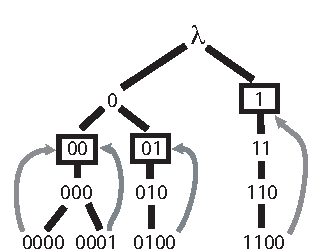
\includegraphics{pics/exthash-tree}
\caption{Reprezentace mno�iny $S$. Vrchol reprezentuj�c� prefix $0$, by ve
sv�m podstrom� m�l 3 prvky, co� je v�ce, ne� po�adujeme pomoc� hodnoty
$b$.}
\label{fig.hash.extern}
\end{figure}

Z obr. \ref{fig.hash.extern} plyne, �e hodnota $d(S) = 2$.
\end{priklad}

\begin{tvrzeni}
Plat�: Kdy� $d(s) = k$ a prvek $t$ m� stejn� prefix d�lky $k$ jako $s$, 
pak $d(s) = d(t)$. 
\end{tvrzeni}

Reprezentace: 
\begin{itemize}
\item adres��: ke ka�d�mu slovu $\alpha$ d�lky $d(S)$ je p�i�azena adresa 
str�nky, kter� obsahuje prvky $s \in S$, �e $h(s)$ m� prefix $\alpha$.
Tato slova d�lky $d(s)$ jsou lexikograficky uspo��d�na.
\item datov� ��st: str�nky s p�i�azen�mi prvky
\end{itemize}

\begin{priklad}
P��klad adres��e pro mno�inu $\{0000, 0001, 0100, 1001 \}$:

\vspace{5mm}

\begin{tabular}{lll}
00 & $\rightarrow$ & 0000, 0001 \\
01 & $\rightarrow$ & 0100 \\
\hline
10 & $\searrow$ & \\
11 & $\rightarrow$ & 1001 \\
\end{tabular}
\end{priklad}

\begin{pozn}
Up�esn�n� reprezentace str�nky (str�nek): \\
Prvek $s \in S$ je ulo�en na str�nce, kter� obsahuje v�echny prvky $t \in
S$ takov�, �e prefix $h(t)$ d�lky $d(s)$ bude je stejn� jako $h(s)$, tato st�nka
bude p�i�azena v�em slov�m $\alpha$ d�lky $d(S)$ takov�m, �e prefix $h(s)$ d�lky
$d(s)$ je prefix $\alpha$. \\
Pokud $\alpha$ neobsahuje ��dn� takov� prefix, tak je mu p�i�azena str�nka
NIL.
\end{pozn}

\subsection{Operace ACCESS}

viz algoritmus \ref{alg:exthash.access}

\begin{algorithm}[!htb]
\caption{ACCESS pro extern� ha�ov�n�}
\label{alg:exthash.access}
ACCESS(x)
\begin{enumerate}
\item Spo��t�me $h(x)$, nat�hneme adres��, nalezneme $d(S)$ a najdeme
str�nky odpov�daj�c� prefixu $h(x)$ d�lky $d(S)$
\item Nat�hneme odpov�daj�c� str�nku do pam�ti, zjist�me, zda obsahuje $x$ a
kdy� ano, provedeme po�adoven� �pravy.
\item Str�nku ulo��me zp�t na stejn� m�sto.
\end{enumerate}
\end{algorithm}

Operace ACCESS vy�aduje 3 p��stupy na extern� medium. (za p�edpokladu, �e
adres�� je tak� ulo�en na extern�m mediu a zab�r� jednu str�nku) 

Pro rychlou implementaci aktualiza�n�ch operac� je vhodn� m�t u ka�d�
str�nky ulo�eno informaci kolik je prvk� na str�nce.


\subsection{Operace INSERT}

viz algoritmus \ref{alg:exthash.insert}

% pozn: \mnote nesmi byt uvnitr prostredi algorithm
\begin{algorithm}[!htb]
\caption{INSERT pro extern� ha�ov�n�}
\label{alg:exthash.insert}
INSERT(x)
\begin{enumerate}
\item Spo��t�me $h(x)$, nat�hneme adres��, nalezneme $d(S)$ a nalezneme adresu
str�nky odpov�daj�c� prefixu $h(x)$ d�lky $d(S)$. (XXX odkud vezmu $d(S)$ ?)
% XXX \mnote{$d(S)$ vezmu odkud ?}
\item Nat�hneme do pam�ti odpov�daj�c� str�nku. kdy� v n� existuje $x$ 
$\rightarrow$ konec
\item Kdy� neobsahuje $x$ a m� m�n� prvk� ne� $b$, vlo��me $x$ do t�to str�nky
a ulo��me ji zp�tky na stejn� m�sto a aktualizujeme adres�� (po�ty prvk�
na str�nce)
\item Kdy� str�nka prvek $x$ neobsahuje a m� $b$ prvk�, str�nku rozd�l�me
(nalezneme nov� $d(s)$ pro $s$ z t�to str�nky i s p�idan�m $x$), str�nky 
ulo��me a aktualizujeme adres��.
\end{enumerate}
\end{algorithm}
\mnote{pokud je nov� nalezen� $d(s) \leq d(S)$, adres�� se zv�t�ovat nebude}

Operace INSERT vy�aduje 6 p��stup� na extern� medium.

\begin{pozn}
Roz�t�pen� str�nky nemus� nutn� znamenat zv�t�en� adres��e.
\end{pozn}

\begin{priklad}
\label{priklad:exthash.insert2}
Do mno�iny z p��kladu \ref{priklad:exthash.tree} vlo��me pomoc� operace
INSERT prvek 1111. Hodnota $d(1100) = 1$ se po vlo�en� prvku 1111
nezm�n�. Podstrom reprezentuj�c� prvky mno�iny $S$ s prefixem 11
bude m�t po vlo�en� prvku 1111 dva syny. (viz obr.
\ref{fig.hash.extern.ins})

\begin{figure}[!htb]
\centering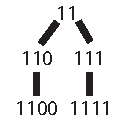
\includegraphics{pics/exthash-ins}
\caption{Podstrom reprezentuj�c� prvky mno�iny $S$ s prefixem 11 po
vlo�en� prvku 1111}
\label{fig.hash.extern.ins}
\end{figure}

Pokud vezmeme situaci danou po vlo�en� prvku 1111, bude adres�� vypadat
takto:

\vspace{5mm}

\begin{tabular}{lll}
00 & $\rightarrow$ & 0000, 0001 \\
\hline
01 & $\rightarrow$ & 0100 \\
\hline
10 & $\searrow$ & 	 \\
  & &  1001 \\
11 & $\nearrow$	& \\
\end{tabular}

\vspace{5mm}

Nyn� vlo��me prvek 0010. V tomto p��pad� dojde ke zv�t�en� adres��e:

\vspace{5mm}

\begin{tabular}{lll}
000 & $\rightarrow$ & 0000, 0001 \\
\hline
001 & $\rightarrow$ & 0010 \\
\hline
010 & $\rightarrow$ & 0100 \\
011 & $\nearrow$ & \\
\hline
100 & $\searrow$ & \\
101 & $\rightarrow$ &  1001, 1111 \\
110 & $\nearrow$ & \\
111 & $\nearrow$ & \\
\end{tabular}

\vspace{5mm}

Hodnota $d(S)$ je nyn� 3.
\end{priklad}


\subsection{Operace DELETE}

viz algoritmus \ref{alg:exthash.delete}

\begin{algorithm}[!htb]
\caption{DELETE pro extern� ha�ov�n�}
\label{alg:exthash.delete}
DELETE(x)
\begin{enumerate}
\item spo��t�me $h(x)$, nat�hneme adres��, nalezneme $d(S)$, nalezneme adresu
str�nky odpov�daj�c� prefixu $h(x)$ d�lky $d(S)$, zjist�me zda po odebr�n�
prvku $x$ m��e nastat spojov�n� str�nek a pokud ano, nalezneme adresu
str�nky, kter� se spoj� s na�� str�nkou
\item nat�hneme odpov�daj�c� str�nku do pam�ti, zjist�me zda obsahuje $x$,
pokud ne, tak konec
\item kdy� obsahuje $x$ a nem��e doj�t ke slou�en� str�nek, tak odstran�me
$x$, str�nku ulo��me na stejn� m�sto a aktualizujeme adres�� (po�ty prvk� na
str�nce)
\item kdy� obsahuje a dojde ke slu�ov�n�, pak odstran�me $x$, nat�hneme
druhou str�nku a str�nky slou��me, ulo��me novou str�nku a aktualizujeme
adres��.
\end{enumerate}
\end{algorithm}
\mnote{pro aktualizaci adres��e to mohou b�t 2 operace - na�ten� a
ulo�en�. z�ejm� proto, aby mohlo b�t sou�asn� pu�t�no v�c operac�.}

\begin{priklad}
Pro situaci z p��kladu \ref{priklad:exthash.insert2} provedeme
DELETE(0100). V adres��i budou pak polo�ky 010 a 011 ukazovat na pr�zdnou
str�nku (NIL). Adres�� z�stal po t�to operaci stejn�.

Nyn� sma�eme prvek 0001.

\begin{figure}[!htb]
\centering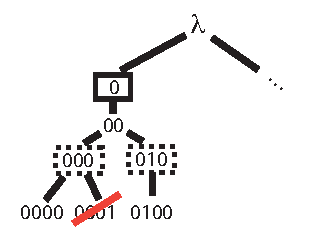
\includegraphics{pics/exthash-del}
\caption{��st stromu reprezentuj�c�ho mno�inu $S$ p�ed smaz�n�m prvku 0001}
\label{fig.hash.extern.del}
\end{figure}

Na obr. \ref{fig.hash.extern.del} je vid�t, �e po smaz�n� prvku 
0001 m��e b�t adres�� op�t zmen�en.

Po proveden� DELETE(0001) bude adres�� vypadat takto:

\vspace{5mm}

\begin{tabular}{lll}
000 & $\rightarrow$ & 0000, 0010 \\
001 & $\nearrow$ & \\
\hline
010 & $\rightarrow$ & NIL \\
011 & $\nearrow$ & \\
\hline
100 & $\searrow$ & \\
101 & $\rightarrow$ &  1001, 1111 \\
110 & $\nearrow$ & \\
111 & $\nearrow$ & \\
\end{tabular}

\vspace{5mm}

Nyn� m��eme prov�st zmen�en� adres��e na:

\vspace{5mm}

\begin{tabular}{lll}
00 & $\rightarrow$ & 0000, 0010 \\
01 & $\nearrow$ & \\
\hline
10 & $\rightarrow$ & 1100, 1111	 \\
11 & $\nearrow$	& \\
\end{tabular}

\vspace{5mm}

Tento adres�� m��eme je�t� zmen�it:

\vspace{5mm}

\begin{tabular}{lll}
0 & $\rightarrow$ & 0000, 0010 \\
\hline
1 & $\rightarrow$ & 1100, 1111 \\
\end{tabular}
\end{priklad}

\begin{pozn}
Pesimistick� odhad pro operaci DELETE je nejv��e 6 p��stup� na extern� 
medium.
\end{pozn}

\subsubsection{Aktualizace adres��e}

V posledn�m kroku DELETE se prov�d� aktualizace adres��e. 
Nejprve provedeme opraven� odkaz� na str�nky: pokud u sud�ho z�znamu v
adres��i dojde k vypr�zdn�n� str�nky, bude tam odkaz na NIL. pokud dojde k
vypr�zdn�n� u lich� str�nky, p�ehod� se odkaz na p�edchoz� (sudou)
str�nku.

Potom se testuje, zda jde adres�� zmen�it. Zmen�ov�n� prov�d�me tak
dlouho, dokud to jde.

\subsection{Reprezentace adres��e}

\begin{itemize}
\item reprezentovat jako posloupnost dvojic (adresa str�nky, po�et prvk� na
str�nce), kde $i$-t� dvojice je p�i�azen� $i$-t�mu slovu v lexikografick�m
uspo��d�n�.
\item zv�t�ov�n� adres��e znamen� zdvojen� prvk�
\item test na zmen�ov�n� adres��e - testujeme, zda adresa na lich�m m�st�
je stejn� jako adresa na n�sleduj�c�m sud�m m�st� - pokud ano, tak zmen��m
adres�� vymaz�n�m sud�ch �len� posloupnosti.
\end{itemize}

O�ek�van� zapln�n� str�nky p�i rovnom�rn�m rozlo�en� dat je 
$b \ln 2 \approx 0.69 b$

O�ek�van� velikost adres��e je $\frac{e}{b \ln 2} n^{1 + \frac{1}{b}}$ (p�i
rovnom�rn�m rozlo�en� dat)

\begin{pozn}
�len $n^{1 + \frac{1}{b}}$ nen� line�rn�, zde je probl�m, proto se to
nehod� pro mal� $b$.
\end{pozn}

\begin{tabular}{|l||l|l|l|l|}
\hline
b/n   	&$10^5$   &$10^6$ 	&$10^8$ 	&$10^{10}$    \\
\hline
2  	&$6.2*10^7$  &$1.96*10^8$	&$1.96*10^{11}$	&$1.96*10^{14}$ \\
10	&$1.2*10^5$  &$1.5*10^6$	&$2.4*10^8$	&$3.9*10^{10}$  \\
50	&$9.8*10^3$  &$1.0*10^6$	&$1.1*10^8$	&$1.2*10^{10}$  \\
100	&$4.4*10^3$  &$4.5*10^4$	&$4.7*10^6$	&$4.9*10^8$   \\
\hline
\end{tabular}

\vspace{5mm}

Jak je vid�t, pro $b = 2$ se to nehod�, adres�� je v�t�� ne� velikost dat.

\begin{pozn}
Kdy� pracujeme s velikost� $S$ kolem $10^{10}$, pak je vhodn�, aby 
$b \geq 100$. Pro v�t�� mno�iny $S$ mus� b�t $b$ v�t��.
\end{pozn}

% --------------------------------------------------------------------------
\section{Perfektn� ha�ov�n�}

Perfektn�m ha�ov�n�m mysl�me �lohu nal�zt pro danou pevnou mno�inu 
$S \subseteq U, |S| = n$ perfektn� ha�ovac� funkci, tj. funkci, kter� nem� na 
mno�in� $S$ kolize. Tato �loha nep�ipou�t� p�irozenou implementaci 
operace INSERT, proto�e p�idan� prvek m��e zp�sobit kolizi. 
Typick� p��klad pou�it� je tabulka kl��ov�ch slov kompil�toru.

\begin{defn}
Funkce $h: U \to \intrange{0}{m-1}$ je perfektn� pro $S$, kdy� je na S
prost� ($\forall x\neq y \in S$ plat� $h(x) \neq h(y)$).
\end{defn}

Za jak�ch podm�nek lze povolit INSERT? Mus� b�t m�lo
pravd�podobn�. Prvky nav�c se d�vaj� jinam a po jist� dob� se v�e
p�epo��t� do jedn� tabulky pro novou perfektn� ha�ovac� funkci.

\begin{samepage}
Po�adavky na hledanou ha�ovac� funkci:
\begin{enumerate}
  \item $h$ je perfektn� na $S$
  \item $\forall x$ je $h(x)$ rychle spo�itateln�
  \item $m$ ��dov� srovnateln� s $n$
  \item zak�dov�n� $h$ vy�aduje m�lo prostoru
\end{enumerate}
\end{samepage}

Po�adavky 2) a 3) jdou proti sob�. A a� se n�m je poda�� skloubit,
budeme m�t probl�my s 4). A nav�c hled�n� $h$ potrv� dlouho.

% ..........................................................................
\subsection{Perfektn� ha�ovac� funkce do tabulky velikosti $n^2$}

Vyu�ijeme, co u� v�me o univerz�ln�m ha�ov�n�. Pro $k \in \intrange{1}{N-1}$ 
a pro pevn� $m$ definujme 
\begin{equation}
h_k(x) = ( kx \bmod N ) \bmod m, \quad\text{kde $N=|U|$ je prvo��slo.}
\end{equation}
Budeme hledat vhodn� $k$, $m$.
Definujme m�ru perfektnosti
\begin{equation}
d = \sum_{k=1}^{N-1} \sum_{x \neq y \in S} \delta_{h_k}(x,y)
\end{equation}
a pro $k \in \intrange{1}{N-1}$ polo�me
\begin{equation}
b_k(i) = |\{ x \in S : h_k(x) = i \}|
\end{equation}

Jednak plat�
\begin{align}
\label{bki2}
% vnitrni suma (s mocninou) dana do zavorky aby byly v poradku priority 
% (from V. Havranek)
d & = \sum_{k=1}^{N-1} \left( ( \sum_{i=0}^{m-1} ( b_k(i) )^2 ) -n \right)\\
\intertext{a tak�}
d & = \sum_{x \neq y \in S} |\{ k : h_k(x)=h_k(y) \}|
	&&\text{prohozen�m sum}\\
\end{align}

Co znamen� $h_k(x) = h_k(y)$ pro $x \neq y$? N�sleduj�c� tvrzen� jsou
ekvivalentn�:
\begin{align*}
kx \bmod N & = ky \bmod N && \pmod m\\
k(x-y) \bmod N & = 0 && \pmod m\\
k(x-y) \bmod N & = r m && \text{pro } r \in 
% *ceil -> *floor (fakticka poznamka od Ladislava Proska
	\{ - \lfloor N/m \rfloor .. \lfloor N/m \rfloor \} - \{0\}, \\
\end{align*}
tedy
\[
d \leq \sum_{x \neq y \in S} 2 \frac Nm = \frac{2 n(n-1) N}m
\]
a dosazen�m do \eqref{bki2}, podle p�ihr�dkov�ho principu
\begin{equation}
\label{existsk}
\exists k : \sum_{i=0}^{m-1} ( b_k(i) )^2 \leq n + \frac{2 n(n-1)}m
\end{equation}

Pro speci�ln� velikosti tabulky dost�v�me dosazen�m do \eqref{existsk}:
\begin{align}
\label{3n}
&\text{Pro } m = n: 
&& \exists k \text{ naleziteln� v �ase }O(nN): 
\sum_{i=0}^{m-1} ( b_k(i) )^2 < 3n\\
\label{perf}
&\text{Pro } m = 1 + n(n-1): 
&& \exists k \text{ naleziteln� v �ase }O(nN):  
h_k \text{ je perfektn�} 
\end{align}

\begin{proof}
Prob�r�me v�echny mo�nosti pro $k$, t�ch je $O(N)$.
\begin{enumerate}
\item[\eqref{3n}]
Pro dan� $k$ spo��t�me $\sum ( b_k(i) )^2$ v �ase $O(n) = O(m)$.
\item[\eqref{perf}]
$\sum ( b_k(i) )^2 \leq n + \frac{2 n(n-1)}{1+ n(n-1)} < n + 2$.
Kdyby $h_k$ nebyla perfektn�, pak 
$\exists j : b_k(j) \geq 2$
a
$\sum ( b_k(i) )^2 \geq (n-2) 1^2 + 1 \cdot 2^2 = n + 2$,
spor.
P�i hled�n� $k$ ov���me perfektnost $h_k$ v �ase $O(n)$.
% zmatek s indexy u k (T. Matousek):
% Tohle by melo byt vporadku. k je jako scitaci index jen v (4.8) a (4.10)
% a dal uz ne.
% Ten soucet v d jde pres vsechny hashovaci funkce a jedna z nich je ta
% prava. Ja bych to tak nechal, je to ok. Staci smazat tu *.
\end{enumerate}
\end{proof}

Nyn� m�me perfektn� ha�ovac� funkci, kter� ale poru�uje po�adavek (3).
% ..........................................................................
\subsection{Perfektn� ha�ovac� funkce do tabulky velikosti $3n$}

Zkombinujeme oba v�sledky z p�edchoz� ��sti.
% --- nejprve prvn� funkc� ha�ujeme do tabulky velikosti $< 3n$

Podle \eqref{3n} nalezneme $k$ takov�, �e
$\sum ( b_k(i) )^2 < 3n$.

Pro ka�d� $i \in \intrange{0}{n-1}$ vezmeme mno�inu koliduj�c�ch prvk�
$S_i = \{ s \in S : h_k(s) = i \}$.
Ozna�me $n_i = |S_i|$.

Podle \eqref{perf} pro ka�d� $i$ nalezneme $k_i$ takov�, �e
pro $m_i = 1 + n_i(n_i-1)$ je $h_{k_i}$ perfektn� pro $S_i$.

Ka�dou zaha�ovanou mno�inu $S_i$ ulo��me ve v�sledn� tabulce od pozice
$d_i$: 
\[
d_i = \sum_{j=0}^{i-1}(1 + n_j(n_j-1)).
\]

Kone�n� definujme
\[
g(x) = d_i + h_{k_i}(x),\quad\text{kde } i = h_k(x),
\]
kter� je perfektn� a velikost tabulky je
\[
m = d_n = \sum_{j=0}^{n-1}(1 + n_j(n_j-1))
\leq \sum_{j=0}^{n-1} n_j^2
=  \sum_{j=0}^{n-1} (b_k(j))^2
< 3n
\]

Ov�em na zak�dov�n� t�to funkce pot�ebujeme hodn� pam�ti: 
nevad� n�m $d_i$, 
ale $k$ a ka�d� $k_i$ je velikosti $O(N)$, 
tedy pot�ebujeme $n \log_2 N$ bit�, co� odporuje na�emu po�adavku (4).
V dal��ch kroc�ch budeme zmen�ovat ��sla definuj�c� ha�ovac� funkci.
% ..........................................................................
\subsubsection{Podobn� funkce dan� ��slem velikosti $O(N)$}

\mnote{lep�� jm�na prom�nn�ch!}
Zvolme prvo��slo $p_1$ takov�, �e 
$1 +n(n-1) \leq p_1 \leq 1+ 2n(n-1)$. N�jak� takov� mus� existovat
(Bertrand�v postul�t: $\forall n>1 \exists$ prov��slo p, �e 
$n < p < 2n$).
Podle \eqref{perf} %TODO, mus�me dok�zat m \geq, co� m�rn� zatemn� dk.
$\exists k : h_k(x) = ( kx \bmod N) \bmod p_1$ 
je perfektn� na $S$.

Vytvo�me
\[
S_1 = \{ h_k(s) : s \in S\} \subset \intrange{0}{p_1 -1}
\]
a na $S_1$ aplikujme p�edchoz� sekci, kde $N = p_1$.

Dost�v�me ha�ovac� funkci $g_1$, kter�
\begin{itemize}
\item je perfektn� pro $S$
\item je spo�itateln� v �ase $O(1)$ 
\item ha�uje do tabulky $<3n$ 
\item je ur�ena 1 ��slem velikosti $O(N)$ \\
 \quad a $O(n)$ ��sly velikosti $O(n^2)$ 
\end{itemize}

% ..........................................................................
\subsubsection{Podobn� funkce dan� ��slem velikosti $O(n^2\log N)$}
Pro extr�mn� p��pady typu $N = 2^{10^6}$ je�t� postup vylep��me,
��m� zmen��me velikost ��sel k�duj�c�ch perfektn� ha�ovac� funkci 
na $O(\log N)$.

\begin{lemma}
\label{n2logN}
Pro ka�dou mno�inu $S \subseteq \intrange{0}{N-1}$ velikosti $n$ existuje
prvo��slo $p$ takov�, �e $f_{p}(x) = x \bmod p$ je perfektn� na
$S$ a $p = O(n^2 \log N)$.
\end{lemma}

Vyu�it�: pro $S$ najdeme prvo��slo $p_0$ velikosti $O(n^2 \log N)$
takov�, �e $f_{p_0}$ je perfektn� na $S$. Vytvo��me 
\[
S_0 = \{ f_{p_0}(s) : s \in S\} \subset \intrange{0}{p_0-1}
\]
a na $S_0$ aplikujme p�edchoz� postup, kde $N = p_0$.

Tedy pro ka�dou mno�inu $S$ velikosti $n$ existuje ha�ovac� funkce $f$, kter�
\begin{itemize}
\item je perfektn� pro $S$
\item je spo�itateln� v �ase $O(1)$ 
\item ha�uje do tabulky $<3n$ 
\item je ur�ena 2 ��sly velikosti $O(n^2 \log N)$ \\
 \quad a $O(n)$ ��sly velikosti $O(n^2)$ 
\end{itemize}

\begin{lemma}
\label{prvociselnidelitele}
Nech� $r$ je ��slo a $p_1, \ldots, p_q$ jsou v�echny jeho prvo��seln�
d�litele. Pak $q=O(\log r / \log\log r)$.
\end{lemma}
\begin{proof}
\begin{align*}
r & \geq \prod_{i=1}^q p_i\\
 & > q! \\
 & = \exp(\sum_{i=1}^q \ln i) \\
 & > \exp(\int_1^q \ln x \,dx) \\
 & \geq {\left( \frac qe \right)}^q \qquad\text{kde } \exp(x)=e^x
\end{align*}
Tedy
\mnote{skok}
\[
q \leq c \frac{\ln r}{\ln\ln r} \quad\text{pro vhodnou konstantu $c$.}
\]
\end{proof}
\begin{proof}[D�kaz lemmatu \ref{n2logN}]
P�edpokl�dejme $S = \{ x_1 < \ldots < x_n \}$.
Ha�ovac� funkce $f_t(x) = x \bmod t$ je perfektn� pr�v� kdy� $t$ je
nesoud�ln� s ��slem
\[
D = \prod_{i>j} (x_i - x_j) < N^{n^2}
\]
Podle \ref{prvociselnidelitele} je mezi prvn�mi $(c \ln D / \ln\ln D)+1$
prvo��sly alespo� jedno, kter� ned�l� $D$. V�me, �e $p_k = O(k \ln
k)$, tedy 
$(c \ln D / \ln\ln D) +1$-n� prvo��slo m� velikost
$O(\ln D) = O( n^2 \ln N)$.
\end{proof}
\mnote{nalezeni prvocisla $p_0$ vyzaduje cas $O(n^2\log N)$.}

% ..........................................................................
\subsection{GPERF}

Jin� konstrukce perfektn� ha�ovac� funkce je pou�ita v programu
{\tt gperf}. Distribuov�n pod GPL. 
Jeho n�vrh je pops�n v \cite{douglas-GPERF}.


% --------------------------------------------------------------------------
\def\xx{% commented out
\section{Ha�ov�n� pro extern� pam�}

\mnote{Tohle u� Koubek nep�edn��} % - zrejme komentar od M.Vidnera
% - sice to Koubek neprednasi (prednasi se to v predmetu OZD), 
% ale u statnic se to zkousi
% Externi hashovani je popsano v jine sekci.
Adres��.

MEMBER, INSERT, DELETE

O�ek�van� zapln�n� str�nky, po�et str�nek, velikost adres��e --- jen
citace, tabulka pro n�kter� ��sla.
}% commented out

% ==========================================================================
% Sou��st skript na Datov� struktury. Viz main.tex
\markright{$ $Id$ $}

\chapter{Trie}

\emph{Trie}\footnote{N�zev \emph{trie} poch�z� z anglick�ho 
"re{\bf trie}val", tedy vyzvednut�. N�zory na to, jak vyslovovat 
"trie" se r�zn�. V �e�tin� se zpravidla vyslovuje tak jak se p��e.} 
je rovinn� implementace slovn�ku.

M�me abecedu $\Sigma$ velikosti $k$. Universum jsou v�echna slova nad
$\Sigma$ d�lky pr�v� $l$ (nekone�nou mno�inu si nem��eme dovolit a
krat�� slova dopln�me zprava mezerami). Chceme reprezentovat mno�inu
slov $S \subseteq U$.


% --------------------------------------------------------------------------

\section{Z�kladn� varianta}

\begin{defn}
\emph{Trie} nad $\Sigma$ je kone�n� strom, jeho� ka�d� vnit�n�
vrchol m� pr�v� $k$ syn�, kter� jsou jednozna�n� ohodnoceny prvky $\Sigma$.
Ka�d�mu vnit�n�mu vrcholu trie odpov�d� slovo nad $\Sigma$ d�lky
nejv��e $l$: ko�enu
odpov�d� pr�zdn� slovo $\Lambda$; kdy� vrcholu $v$ odpov�d� slovo
$\alpha$, pak $v[a]$, synu $v$ ohodnocen�mu p�smenem $a$, odpov�d�
slovo $\alpha a$.
\end{defn}

\newcommand{\Nal}{\textrm{Nal}}
\begin{defn}
�ekneme, �e trie nad $\Sigma$ \emph{reprezentuje mno�inu} $S$, kdy�:
\begin{itemize}
  \item List�m je p�i�azena boolovsk� funkce n�le�en� \Nal: $\Nal(t)$ je
  	true pr�v� kdy� slovo, kter� odpov�d� listu $t$, je v $S$.
  \item (\emph{prefixov� podm�nka}) Kdy� $v$ je vnit�n� vrchol trie 
	odpov�daj�c� slovu $\alpha$, pak
  	existuje $\beta \in S$ takov�, �e $\alpha$ je prefix $\beta$.
  \item Pro ka�d� slovo $\alpha \in S$ existuje v trie list odpov�daj�c�
  	$\alpha$.
\end{itemize}
\end{defn}

% podle http://en.wikipedia.org/wiki/Trie
\begin{pozn}
Na rozd�l od bin�rn�ho vyhled�vac�ho stromu (viz kapitola~\ref{bvs},
sekce~\ref{bvs:obecne}), ��dn� vrchol ve strom� neobsahuje ulo�en� kl��,
kter� reprezentuje. Nam�sto toho jeho pozice ve strom� ud�v� kl��, kter�
reprezentuje\footnote{Tato a n�sleduj�c� pozn�mka jsou voln� p�evzaty z
encyklopedie Wikipedia, heslo Trie.}. 
Pouze n�kter� vrcholy ve strom� obsahuj� data - nap�. pro
implementaci slovn�ku s hesly by data ulo�en� v listech obsahovala popis
tohoho hesla\footnote{Nap�. slovn�k spisovatel�, kde listy ve trie by
odpov�daly jm�n�m jednotliv�ch spisovatel� a data ulo�en� v nich by 
obsahovala seznam jejich d�l.}.
\end{pozn}

% podle http://en.wikipedia.org/wiki/Trie
\begin{pozn}
Pro� jsou trie v�hodn� ?

\begin{itemize}
  \item Vyhled�v�n� kl��� je rychlej�� ne� v BVS. Vyhled�n� kl��e d�lky
  $m$ vy�aduje pouze $O(m)$ �asu. Pro BVS je to $O(m^2)$ v nejhor��m p��pad�,
  proto�e se mus� opakovan� porovn�vat po��te�n� znaky hledan�ho slova.
  Dal�� v�hoda je pou�it� indexace pomoc� znak� v operaci MEMBER.
  \item Trie zab�raj� m�n� m�sta. Proto�e nejsou kl��e v trie ulo�eny
  explicitn�, pro ulo�en� jednoho kl��e je pot�eba pouze amortizovan�
  konstantn� prostor.
  \item Pomoc� trie lze jednodu�e prov�d�t operaci hled�n� nejdel��ho 
  prefixu\footnote{anglicky ``longest-prefix matching``}, kde pot�ebujeme
  naj�t kl��, kter� m� nejdel�� shodn� prefix s hledan�m
  kl��em\footnote{To se hod� nap��klad pro implementace s��ov�ch
  opera�n�ch syst�m�, kde je pot�eba prov�d�t tuto operaci pro
  hled�n� v routovac�ch tabulk�ch nebo tabulk�ch pro p�eklad adres. 
  V p��pad� sm�rovac�ch tabulek se pos�l� paket na dal�� "hop" podle 
  c�lov� adresy. Routovac� tabulka obsahuje z�znamy, kter� ud�vaj� adresu
  s�t� a adresu za��zen�, na kter� pos�lat pakety pro tuto s�� - tzv.
  "hop". Tento "hop" se vyb�r� tak, aby c�lov� adresa paketu m�la
  co mo�n� nejdel�� shodn� prefix s n�jakou adresou s�t� v routovac�
  tabulce.}. 
  D�le trie dovoluj� asociovat jednu hodnotu s mno�inou kl���, kter� maj�
  shodn� prefix\footnote{T�m, �e ulo��me data do vnit�n�ch uzl� trie.}.
\end{itemize}
\end{pozn}

% ..........................................................................
\subsection{Algoritmus MEMBER}

viz algoritmus \ref{alg:trie.member}.

\begin{algorithm}[!htb]
\caption{MEMBER pro z�kladn� verzi trie}
\label{alg:trie.member}
\begin{algorithmic}
\STATE \COMMENT {vyhled�n� $x = x_1 \dots x_l$}
\STATE $t := \text{ko�en}$
\STATE $i := 1$
\WHILE {$t \text{ nen� list}$}
        \STATE $t := t[x_i]$ // sestup podle znaku $x_i$
        \STATE $i := i + 1$
\ENDWHILE
\STATE \COMMENT {test}
\STATE \textbf{return} $\Nal(t)$
\end{algorithmic}
\end{algorithm}

Na tomto algoritmu je zaj�mav� to, �e pou��v� jednotliv� znaky hledan�ho
slova $x$ k indexaci v jednotliv�ch vrcholech trie (viz ��dek s
koment��em ve v�pisu algoritmu~\ref{alg:trie.member}.). To dovoluje naj�t
vrchol do kter�ho se m� p�i hled�n� sestoupit v �ase $O(1)$. Tedy
slo�itost operace MEMBER je $O(l)$, proto�e mus�me proj�t nejv��e $l$
vrchol� ne� dos�hneme listu (d�lka slov je nejv��e $l$).

% ..........................................................................
\subsection{Algoritmus INSERT}

viz algoritmus \ref{alg:trie.insert}.

\begin{algorithm}[!htb]
\caption{INSERT pro z�kladn� verzi trie}
\label{alg:trie.insert}
\begin{algorithmic}
\STATE \COMMENT {vyhledej $x$ pomoc� operace MEMBER(x)}
\IF[trie nemus� b�t tak hlubok�, jak pot�ebujeme] {\textbf{not} $\Nal(t)$}
        \WHILE {$i \leq l$}
                \STATE vrcholu $t$ p�idej $k$ list� ohodnocen�ch
                p�smeny z $\Sigma$, jejich $\Nal := \textit{false}$
                \STATE $t := t[x_i]$
                \STATE $i := i + 1$
        \ENDWHILE
        \STATE $\Nal(t) := \textit{true}$
\ENDIF
\end{algorithmic}
\end{algorithm}

P�i operaci INSERT se sestupuje a� na �rove� d�lky slova, p�i�em� se
p�id�vaj� nov� �rovn� v p��pad� �e nejsou v trie p��tomny\footnote{Celkem 
hezky si lze proces p�id�v�n� nov�ch hladin v r�mci jedn� v�tve p�edstavit 
tak, �e v ka�d� hladin�, kter� je nov� p�idan�, "vyroste smet�k" s $k$ 
vrcholy.}.

% ..........................................................................
\subsection{Algoritmus DELETE}

viz algoritmus \ref{alg:trie.delete}.

\begin{algorithm}[!htb]
\caption{DELETE pro z�kladn� verzi trie}
\label{alg:trie.delete}
\begin{algorithmic}
\STATE \COMMENT {vyhledej $x$ pomoc� operace MEMBER(x)}
\IF {$\Nal(t)$}
        \STATE $\Nal(t) := \textit{false}$
        \STATE $t := \text{otec } t$
        \STATE \COMMENT {oprav�me prefixovou podm�nku}
        \WHILE {v�ichni synov� $t$ jsou listy s $\Nal = \textit{false}$}
                \STATE zru� listy $t$
                \STATE $\Nal(t) := \textit{false}$
                \STATE $t := \text{otec } t$
        \ENDWHILE
\ENDIF  
\end{algorithmic}
\end{algorithm}

Analogicky k operaci INSERT doch�z� k ru�en� hladin v r�mci jedn� v�tve
v p��pad� �e v�echny
listy v hladin� maj� hodnotu $\Nal = \textit{false}$.

Pou�ili jsme obrat $t := \text{otec } t$. To lze prov�st bu� tak, �e
se vrchol krom� sv�ch syn� odkazuje i na sv�ho otce a spot�ebuje tak
pam� nav�c, nebo se cesta z ko�ene do aktu�ln�ho vrcholu b�hem
sestupu ve stromu pamatuje na z�sobn�ku. Tento trik se pou��v� u 
v�ech stromov�ch struktur.

% ..........................................................................
\subsection{�asov� a pam�ov� slo�itost}

Jedna iterace cyklu zabere konstantn� �as. �as pro MEMBER je $O(l)$,
�as pro INSERT a DELETE je $O(l k)$. Pam�ov� slo�itost trie v nejhor��m
p��pad� je po�et
ulo�en�ch slov n�soben� d�lkou cesty a po�tem syn�, tedy $O(|S| l k)$.

\begin{pozn}
V p��pad�, kdy S obsahuje (skoro) v�echna slova d�lky $l$, tak m��e
m�t slo�itost jen $O(|S|)$.
\end{pozn}

% --------------------------------------------------------------------------
\section{Komprimovan� trie}

M�jme $\Sigma = \{0,1,2\}$, $l=7$.
$S = \{0202011, 0202012, 0202021, 1212102, 1212111, 1212121, 1212122\}$.
Nekomprimovan� trie pro tuto mno�inu je na obr�zku \ref{fig:tries}.
Vid�me, �e p�smena na druh� a� p�t� pozici jsou v�dy stejn� a
% XXX \uv{prokousat} 
p�edchoz� algoritmy se jimi mus� prokousat. P�esn�ji 
�e�eno, prohl��en� vrcholu $v$, kter� m� jedin�ho 
syna, kter� nen� list s hodnotou $\Nal = \textit{false}$, nep�in�� 
��dnou kladnou informaci, proto�e mno�iny prvk� z $S$, 
kter� jsou reprezentov�ny vrcholy v podstromu otce $v$ a v podstromu 
vrcholu $v$ jsou stejn�. To vedlo k idei tyto vrcholy ze stromu vynechat a
t�m zmen�it (komprimovat) trie.  

\begin{figure}
\centering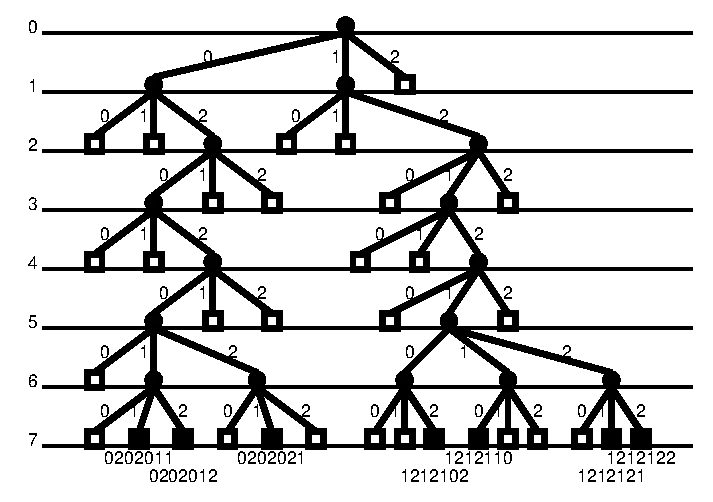
\includegraphics{pics/tries}
\caption{Nekomprimovan� trie. �ern� vypln�n� �tverce zn�zo�uj� listy,
kter� odpov�adj� n�jak�mu slovu z (reprezentovan�) mno�iny $S$. Tyto listy
maj� hodnotu funkce Nal \textit{true}. B�le vypln�n� �tverce ��dn�mu slovu
ze $S$ neodpov�daj�, maj� tedy hodnotu Nal \textit{false}.}
\label{fig:tries}
\end{figure}

\newcommand{\uro}{\textrm{uroven}}
Ke ka�d�mu vrcholu $v$ p�id�me funkci $\uro(v)$ vyjad�uj�c� ��slo �rovn�,
ve kter� se $v$ nach�z� v p�vodn�m trie.
\newcommand{\slo}{\textrm{slovo}}
Ke ka�d�mu listu $v$ p�id�me funkci $\slo(v)$ --- slovo, kter� odpov�d� $v$.

Nyn� m��eme vynech�vat vrcholy podle n�sleduj�c�ho krit�ria: 
je-li $v$ vnit�n� vrchol a v�ichni jeho synov� krom� $w$ jsou listy s
$\Nal = \textit{false}$, pak $v$ vynech a za�a� $w$ na jeho m�sto. Tento proces 
opakujeme dokud trie obsahuje n�jak� vnit�n� vrchol, jeho� v�ichni synov� 
s v�jimkou jednoho jsou listy, pro n� $\Nal = \textit{false}$. 
V�imn�te si, �e ka�d� vnit�n� vrchol m� pr�v� $k$ syn�, kter� jsou 
v jednozna�n� korespondenci s p�smeny abecedy $\Sigma$.

\begin{priklad}
Nech� $\Sigma = \{0,1,2\}$, $l=3$.
$S = \{ 001,102,010,211,212 \}$.

Nekomprimovan� trie pro mno�inu $S$ a jeho komprimovan� varianta je na
obr. \ref{fig:tries.compr1}.

\begin{figure}
\centering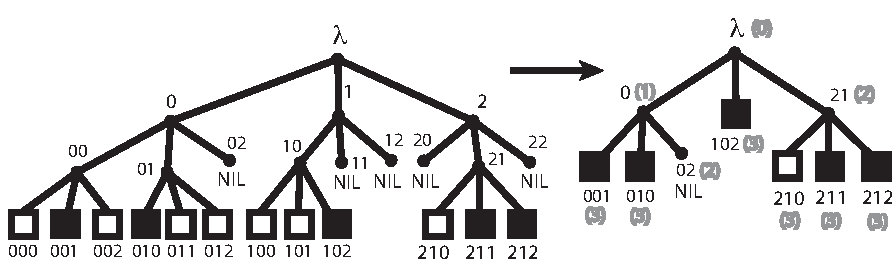
\includegraphics{pics/trie-compr1}
\caption{Komprimace trie. �ed� ��sla v z�vorce zna�� hodnotu $uroven()$}
\label{fig:tries.compr1}
\end{figure}

\end{priklad}


\begin{pozn}
\mnote{Koubek 2002/2003}
Komprimovan� trie je tvo�en� mno�inou vrchol�, kde pro $\beta$ je
$hladina(\beta) = |\beta|$ a otec $\beta$ je nejv�t�� vlastn� prefix,
kter� pat�� do trie + p�idan� listy. Listy jsou prvky z S + slova $\beta
a$, kde $\beta \in$ trie a $\beta a$ nen� prefixem ��dn�ho slova v $S$. 
Pro prvky z $S$ je Nal = True, jinak false. 
Plat� $prvek(\gamma) = \gamma$ pro ka�d� list.

Kdy� $\beta \in$ trie a $a \in \Sigma \rightarrow$
$\Bigl\{$
\begin{tabular}{ll}
$\beta a$ list, & je $a$-t�m synem $\beta$ \\
$\exists \delta \in S$, & �e $\beta a$ je prefixem $\delta$
\end{tabular}

Potom $a$-t� syn $\beta$ je nejkrat�� prefix v mno�in� trie v $S$, kter�
obsahuje $\beta a$.
\end{pozn}

% ..........................................................................
\subsection{MEMBER}

Viz algoritmus \ref{alg:trie.k.mem}

\begin{algorithm}[!htb]
\caption{MEMBER pro komprimovan� trie}
\label{alg:trie.k.mem}
\begin{algorithmic}
\STATE \COMMENT {vyhled�n� $x = x_1 \ldots x_l$}
\STATE $t := \text{ko�en}$
\WHILE {$t \text{ nen� list}$}
        \STATE $i := \uro(t) + 1$
        \STATE $t := t[x_i]$ // $x_i$-t� list
\ENDWHILE
\STATE \COMMENT {test}
\STATE \textbf{return} $\Nal(t) \land \slo(t) = x$
\end{algorithmic}
\end{algorithm}

% XXX zde \mnote{n�co chyb�}

% ..........................................................................
\subsection{INSERT}

Viz algoritmus \ref{alg:trie.k.ins}

\begin{algorithm}
\caption{INSERT pro komprimovan� trie}
\label{alg:trie.k.ins}
\begin{algorithmic}
\STATE \COMMENT {vyhledej $x$}
\IF {$\Nal(t) \land \slo(t) = x$}
	\STATE \COMMENT {Trie u� obsahuje $x$, ned�lej nic.}
\ELSE
        \IF {$\slo(t) = x$}
		\STATE \COMMENT {Trie obsahuje spr�vn� list,
		pouze nastav p��znak. Nap�. "0202010"}
                \STATE $\Nal(t) := \textit{true}$
	\ELSE
		\STATE \COMMENT {Bude pot�eba vlo�it nov� list.}
		\STATE \COMMENT {Najdi, kam ho p�ipojit.}
                \STATE $\alpha$ := nejdel�� spole�n� prefix slov
		$x$ a $\slo(t)$. D�lku $\alpha$ ozna�me $|\alpha|$.
                \STATE $v$ := vrchol na cest� z ko�ene do $t$ takov�,
                �e $\uro(v)$ je nejv�t��, kter� je $\leq |\alpha|$
                \IF {$\uro(v) = |\alpha|$}
                        \STATE \COMMENT {$v$ je otec nov�ho listu}
		\ELSE[$\uro(v) < |\alpha|$]
                        \STATE \COMMENT {Bude pot�eba vytvo�it
			otce nov�ho listu}
                        \STATE $a$ := $\uro(v)+1$-n� p�smeno $\alpha$
                        \STATE $u := v[a]$
                        \STATE \COMMENT {Mezi $v$ a $u$ vytvo� nov�
			vnit�n� vrchol odpov�daj�c� slovu $\alpha$}
                        \STATE $w$ := nov� vrchol, $\uro(w) := |\alpha|$
                        \STATE $v[a] := w$
                        \STATE $c$ := $|\alpha|+1$-n� p�smeno $\slo(t)$
                        \STATE $w[c] := u$
                        \FORALL {$b \in \Sigma, b \neq c$}
                             \STATE $z$ := nov� vrchol, $\uro(z) := |\alpha|+1, \Nal(z) := \textit{false}, \slo(z) := \alpha b$, 
                             \STATE $w[b] := z$
                        \ENDFOR
                        \STATE $v := w$
                \ENDIF
		\STATE \COMMENT {Spr�vn�mu listu p�i�a� $x$}
		\STATE $d$ := $|\alpha|+1$-n� p�smeno $x$
                \STATE $s := v[d]$
                \STATE $\uro(s) := l, \Nal(s) := \textit{true}, \slo(s) := x$
        \ENDIF
\ENDIF
\end{algorithmic}
\end{algorithm}

% ..........................................................................
\subsection{DELETE}

Viz algoritmus \ref{alg:trie.k.del}

\begin{algorithm}[!htb]
\caption{DELETE pro komprimovan� trie}
\label{alg:trie.k.del}
\begin{algorithmic}
\STATE \COMMENT {vyhledej $x$}
\IF {$\Nal(t) \land \slo(t) = x$}
        \STATE $u$ := otec $t$
        \STATE $i := \uro(u)$
        \STATE $\Nal(t) := \textit{false}$
        \STATE $\uro(t) := i+1$, $\slo(t)$ := prefix slova $x$ d�lky $i+1$
        \STATE \COMMENT {vrchol $u$ m� alespo� jednoho syna, kter� nen� list s $\Nal = \textit{false}$}
        \IF {v�ichni synov� $u$ krom� syna $w$ jsou listy s $\Nal = \textit{false}$}
                \STATE $v$ := otec $u$
                \STATE sma� $u$ a v�echny syny $u$ krom� $w$
                \STATE $j := \uro(v) + 1$
                \STATE $v[x_j] := w$ // $x_j$-t� syn $v$ je $w$
        \ENDIF
\ENDIF  
\end{algorithmic}
\end{algorithm}

% ..........................................................................
\subsection{�asov� a pam�ov� slo�itost}

Pam�ov� slo�itost takto komprimovan�ch trie je $O(nk)$, kde 
% oprava by Ladislav Prosek O(nl + kl) -> O(nk)
$n$ je velikost reprezentovan� mno�iny. (maxim�ln� $n-1$ vnit�n�ch vrchol�,
ka�d� s polem d�lky $k$).
�asov� slo�itost operace MEMBER je v nejhor��m
p��pad� $O(l)$, pro INSERT a DELETE je to $O(l+k)$. 
(m��e b�t nutn� p�idat/odebrat jeden vnit�n� vrchol).
% oprava slozitosti v nejhorsim pripade by Ladislav Prosek 

V pr�m�rn�m p��pad� (za p�edpokladu rovnom�rn�ho
rozlo�en� vstupn�ch dat) je to o�ek�van� hloubka trie. Tu
te� spo��t�me.

Nech�
\[
q_d = \pr(\text{trie m� hloubku alespo� $d$})
\]
O�ek�van� hloubka trie reprezentuj�c� $n$ slov je
\[
E_n = \sum_{d=0}^\infty d (q_d - q_{d+1}) = \sum_{d=0}^\infty q_d
\]
Kdy� funkce $\text{pref}_{d-1}$, p�i�azuj�c� slovu 
$\alpha$ jeho prefix d�lky $d-1$, je na mno�in� $S$ prost�,
pak trie reprezentuj�c� mno�inu $S$ m� hloubku nejv��e $d$.
Spo��t�me po�et mno�in o velikosti $n$, na nich� je funkce $\text{pref}_{d-1}$ 
prost�. Tyto mno�iny z�sk�me tak, �e vybereme $n$ prefix� d�lky $d-1$
a ka�d� dopln�me v�emi sufixy d�lky $l-d+1$. Proto t�chto mno�in je
\[
\binom{k^{d-1}}{n} k^{n (l-d+1)}.
\]
Proto�e v�ech podmno�in velikosti $n$ je $\binom{k^l}{n}$ dost�v�me, �e 
\begin{align*}  
q_d 
 &\leq 1 - \frac{\binom{k^{d-1}}{n} k^{n (l-d+1)}}{\binom{k^l}{n}} 
\Biggl\} \text{pravd�podobnost} \\
 &\leq 1 - \frac{k^{d-1}(k^{d-1}-1)\dots(k^{d-1}-(n-1)) k^{n(l-d+1)}}{k^{ln}}\\
 &   = 1 - \prod_{i=0}^{n-1} \left( 1 - \frac{i}{k^{d-1}} \right) \\
 &\leq 1 - \exp\left( \frac{-n^2}{k^{d-1}} \right)\\
 &\leq \frac{n^2}{k^{d-1}},
\end{align*}
pon�vad�
\begin{align*}
                  \prod_{i=0}^{n-1}    \left( 1 - \frac{i}{k^{d-1}} \right)
 &   = \exp\left( \sum_{i=0}^{n-1} \ln \left( 1 - \frac{i}{k^{d-1}} \right)
	   \right)\\
 &\geq \exp\left(         \int_0^n \ln \left( 1 - \frac{i}{k^{d-1}} \right)
	   \right)\\
 &   = \exp\left( \frac{-n^2}{k^{d-1}} \right),
\end{align*} 
(u�ijte integr�ln� kriterium a substituci $x = k^{d-1}(1-t)$) a 
$e^x - 1 \geq x$ (odtud $1 - e^x \leq -x$). 
Tedy pro $c = 2\lceil \log_kn\rceil$ dost�v�me

\begin{align*}
E_n
 & = \sum_{d=1}^cq_d + \sum_{d=c+1}^{\infty}q_d\\
 &\leq c + \sum_{d=c}^{\infty}\frac{n^2}{k^d}\\
 &\leq 2\lceil\log_kn\rceil +
		\left( \frac{n^2}{k^c} \right) \sum_{d=0}^{\infty} k^{-d}\\
 &\leq 2\lceil\log_kn\rceil + \frac{1}{1-1/k}\\
 & = 2\lceil\log_kn\rceil + \frac{k}{k-1}.
\end{align*}

Tedy o�ek�van� �as operace MEMBER je $O(\log_k(n))$ ($O(\frac{\log n}{\log
k})$)
a $O(\log_k(n) + k)$ pro INSERT a DELETE
\mnote{L.Pro�ek: Mo�n� v t� o�ek�van� slo�itosti by �lo +k zanedbat, ale
ne na z�klad� toho tvrzen�, kter� dokazuje jen o�ek�vanou hloubku}
pro komprimovan� trie (za p�edpoklad� rovnom�rn�ho rozlo�en� vstupn�ch dat) 
Zde parametr $k$ vyjad�uje vztah mezi prostorov�mi 
a �asov�mi n�roky.

% . . . .. . . .. .. .. . .  . .. .. .. . . ..  ..  .... . . .. . .. . .
% nasledujici sekci (jeste kompr. trie atd.) dopsal Vladimir Kotal, 2003

\begin{algorithm}[!htb]
	\caption{INSERT pro komprimovan� trie, analogie \ref{alg:trie.k.ins} (verze Koubek 2002)}
\label{alg:trie.k.ins_unk}
\begin{algorithmic}
\STATE INSERT($x=x_1, ..., x_l$)
\STATE $t$ $\leftarrow$ ko�en
\WHILE {$t$ neni list}
  \STATE i $\leftarrow$ hladina($t$), $t$ $\leftarrow$ $(a_{i+1})$-n� syn $t$
\ENDWHILE
\IF {prvek($t$) neni prefix $x$}
  \STATE $\beta$ = nejv�t�� spole�n� prefix $x$ a prvek(t)
  \STATE $\beta a$ = prefix $\alpha$
  \STATE $\beta b$ = prefix prvek($t$)
  \STATE while $hladina(t) > |beta|$ do t $\leftarrow$ otec(t) done
  \IF {$hladina(t) < |\beta|$}
    \STATE vytvo��me nov� vrchol $w$, jeho� synov�, krom� $b$-t�ho syna budou listy s
    \STATE funkcemi Nal = false
    \STATE $prvek(t) = \beta$ + oznaceni syna
    \STATE $hladina(w) = |\beta|, \beta = (a_1, ..., a_i)$
    \STATE necht $v = a_{hladina(t) + 1}$ - t� syn t, b-t� syn w je v
    \STATE $w = a_{hladina(t)+1}$-t� syn t
  \ENDIF
  \STATE z $\leftarrow$ a-t� syn $t$, Nal($z$) = true, prvek($z$) = $x$
\ELSE
  \STATE Nal(t) = true, prvek(t) = $x$
\ENDIF
\end{algorithmic}
\end{algorithm}


\mnote{XXX dalsi neznamy algoritmus z prednasky 2002}
\begin{algorithm}[!htb]
\caption{DELETE pro komprimovan� trie (?)}
\label{alg:trie.k.del_unk}
DELETE($x=x_1, ..., x_l$)
\begin{algorithmic}
\STATE t $\leftarrow$ ko�en
\WHILE {t neni list}
  \STATE i $\leftarrow$ hladina(t), t $\leftarrow$ $(a_{i+1}$-ni syn t
\ENDWHILE
\IF {Nal(t) = true a prvek(t) = j} 
  \STATE Nal(t) = false
  \STATE v $\leftarrow$ otec(t)
  \STATE prvek(t) $\leftarrow$ prefix prvek(t) o d�lce hladina v+1
  \IF {vsichni synove vrchovlu v az na jednoho jsou listy s Nal = false}
    \STATE w $\leftarrow$ syn(v), ktery je bud list s Nal(w) = true nebo neni list
    \STATE necht v je a-t� ($a_i$-ty ???) syn sv�ho otce, v sma�eme a sma�eme
    \STATE v�echny syny $v \neq w$
    \STATE w $\leftarrow$ a-t� ($a_i$-t� ???) syn otce v
  \ENDIF
\ENDIF
\end{algorithmic}
\end{algorithm}


\section{Je�t� komprimovan�j�� trie}

% XXX dopsat !
\begin{priklad}
\label{example.trie.yetmorecompr}

\begin{figure}[!htb]
\centering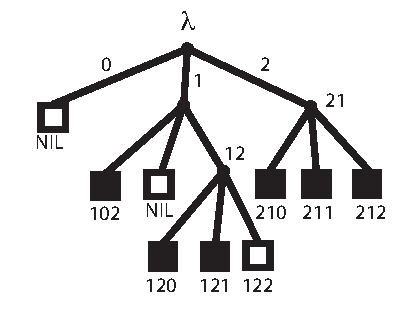
\includegraphics{pics/trie-compr2}
\caption{Nekomprimovan� trie pro p��klad \ref{example.trie.yetmorecompr}}
\label{fig.trie.compr}
\end{figure}

M�jme komprimovan� trie z obr. \ref{fig.trie.compr}
a jeho matici: 

\hspace{5mm}

\begin{tabular}{|l|l|l|l|}
\hline
 & 0 & 1 & 2 \\
\hline
root & NIL & a & b \\
a & 102 & NIL & c \\
b & 210 & 211 & 212 \\
c & 120 & 121 & NIL \\
\hline
\end{tabular}
\end{priklad}

\hspace{5mm}

Chceme se zbavit polo�ek NIL v matici reprezentuj�c� trie. Dal�� komprese
dos�hneme pomoc� vektor� $hod$ (vektor hodnot) a $rd$. Tyto vektory budou
reprezentovat p�vodn� matici.

\mnote{co znamena $rd$ ?}

\subsection{Popis $A$ a $rd$}

Zp�t k na�emu p��kladu:

\begin{enumerate}
\item
  \begin{tabular}{|l|llllll|}
  \hline
  hod & 210 & 211 & 212 & 120 & 121 & NIL \\
  \hline
  \end{tabular}
  
  \hspace{2mm}
  
  \begin{tabular}{|l|llll|}
  \hline
     & root & a & b & c \\
  \hline
  rd &      &   & 0 & 3 \\
  \hline
  \end{tabular}
  
  % \hspace{5mm}
  
\item  
  \begin{tabular}{|l|llllllllll|}
  \hline
  hod & 210 & 211 & 212 & 120 & 121 & a & b & 102 & NIL & c \\
  \hline
  \end{tabular}
  
  \hspace{2mm}
  
  \begin{tabular}{|l|llll|}
  \hline
     & root & a & b & c \\
  \hline
  rd & 4    & 7 & 0 & 3 \\
  \hline
  \end{tabular}
\end{enumerate} 
%  \hspace{5mm}

��dek $i$ za��n� na m�st� $rd(i)$ a mus� b�t spln�na podm�nka: \\
Kdy� $M_{i,j} \neq NIL \neq M_{i',j'}$, pak $rd(i) + j \neq rd(i') + j'$ \\
Kdy� na m�st� hod chceme zapsat prvek $\neq NIL$ a NIL, pak zap��eme prvek
$\neq NIL$.

% ------------------------------------------------------------------------

\subsection{Algoritmus pro hled�n� rd a hod}

% XXX r x s
Nech� $M$ je matice typu $r x s$, m� $m$ v�znamn�ch m�st $\neq$ NIL.

\begin{itemize}
\item pro ka�d� ��dek nalezneme po�et m�st $\neq$ NIL
\item set��d�me ��dky Bucketsortem, tak �e r�dky s~v�t��m po�tem m�st
 $\neq$ NIL p�edch�zej� ��dky s men��m po�tem m�st $\neq$ NIL
\item proch�z�me ��dky v dan�m set��d�n� a pro ka�d� ��dek $i$ nalezneme
  nejmen�� ��slo $rd(i)$, �e nedoch�z� ke kolizi s p�edchoz�mi ��dky (tj.
  kdy� $M_{i',j'} \neq NIL \neq M_{i,j}$) a ��dek $i'$ byl za�azen, pak
  $rd(i) + j \neq rd(i') + j'$.
  Pak $M_{i,j} \neq NIL$ je ulo�eno ve vektoru hod na m�st� $rd(i)+j$.
\end{itemize}

$m(l)$ - po�et m�st $\neq$ NIL v ��dc�ch s po�tem m�st $\geq l+1 \neq NIL$.

\begin{theorem}
Kdy� $m(l)(l+1) \leq m$ pro ka�d� $l$, pak $rd(i) < m$ pro ka�d� ��dek $i$
a algoritmus vy�aduje �as $O(rsm)$.
\end{theorem}

\begin{proof}
P�edpokl�dejme, �e hled�me rd pro ��dek $i$, kter� m� l m�st $\neq NIL$. \\
ve vektoru hod je obsazeno m�n� ne� $m(l-1)$ m�st. \\ 
zkou��me $rd(i)=1,2,...$ \\
$rd(i) = 1,2,...$ je zak�zan�, kdy� vznikne kolize. \\
tj. $\exists$ ��dek $i'$ p�edch�zej�c� a $\exists j,j'$ takov�, �e
$M_{i',j'} \neq NIL \neq M_{i,j}$ 
a platilo by $rd(i') + j' = rd(i) + j$.
$\rightarrow$ t�chto mo�nost� je $< lm(l-1) \leq m$. \\
$O(rs)$ - zjist�me pro ka�d� ��dek po�et m�st $\neq NIL$. \\
$O(m+r)$ - t��d�n� Bucketsortem \\
$O(mrs)$ - krok 2
\end{proof}

%jedna mo�nost
%% XXX obr. matice
%M = 
%$\rightarrow$ budeme m�t moc ��dk� - nevhodn�

\begin{priklad}
XXX nejaky komentar \\

\vspace{5mm}

\begin{tabular}{|l|lll|}
\hline
M & 0 & 1 & 2 \\
\hline
root & NIL & a & b \\
a & 102 & NIL & c \\
b & 210 & 211 & 212 \\
c & 120 & 121 & NIL \\
\hline
\end{tabular}

\vspace{5mm}

\begin{tabular}{|l|llll|}
\hline
    & root & a & b & c \\
\hline
rd  &    4 & 7 & 0 & 3 \\
\hline
\end{tabular}

\vspace{3mm}

\begin{tabular}{|l|llllllllll|}
\hline
hod & 210 & 211 & 212 & 120 & 121 & a & b & 102 & NIL & c \\
\hline
\end{tabular}

\vspace{3mm}

\begin{tabular}{|l|lll|}
\hline
M' & 0 & 1 & 2 \\
\hline
b & 210 & 211 & 212 \\
c & 120 & 121 & NIL \\
root & NIL & a & b \\
a & 102 & NIL & c \\
\hline
\end{tabular}

\hspace{3mm}

(p�ehodili jsme pouze ��dky)

$sl$ - vektor posunut�ch sloupc�

\begin{itemize}
\item $sl(0) = 0$
\item $sl(1) = 1$
\end{itemize}

\begin{tabular}{|l|lll|}
\hline
M' & 0 & 1 & 2 \\
\hline
1 & 210 & NIL & NIL \\
2 & 120 & 211 & 212 \\
3 & NIL & 121 & NIL \\
4 & 102 & a & b \\
5 & NIL & NIL & c \\
\hline
\end{tabular}

\hspace{5mm}

\begin{tabular}{l}
$zac = (6,0,6,3,6)$ \\
$hod = (120, 211, 212, 102, a, b, 210, 121, c)$
\end{tabular}

Kdy� $M(i,j)$ je v�znamn� m�sto, pak $M(i,j) = hod(zac(i+sl(j)) + j)$.

\subsection{Vertik�ln� posun sloupc�}

$cd$ - vektor sloupcov�ho posunut�, slou�� k z�pisu transformace

\vspace{5mm}

\begin{tabular}{|l|lll|}
\hline
   & 0 & 1 & 2 \\
\hline
cd & 0 & 1 & 2 \\
\hline
\end{tabular}
\par

\vspace{5mm}

\begin{tabular}{|l|lllll|}
\hline
   & 0 & 1 & 2 & 3 & 4 \\
\hline
rd & 6 & 0 & 6 & 3 & 6 \\
\hline
\end{tabular}
\par

\vspace{5mm}

\begin{tabular}{|l|lllllllll|}
\hline
hod & 120 & 211 & 212 & 102 & a & b & 210 & 121 & c \\
\hline
\end{tabular}

\hspace{3mm}

\end{priklad}

Jak najdeme nazp�tek m�sta ? Plat�, kdy� $M_{i,j} \neq NIL$, pak
$hod(rd(i+cd(j)+j)) = M_{i,j}$
\mnote{je ten vzorec spr�vn� ?}

\par
{\em zna�en�:} 
\begin{itemize}
\item f(-,-) je fce dvou prom�nn�ch 
\item $B_j$ matice posunut�ch prvn�ch sloupc� 
\item $m_j$ po�et m�st $\neq NIL$ v $B_j$ 
\item $m_j(l)$ po�et m�st $\neq NIL$ v ��dc�ch matice $B_j$, kter� maj� aspo� l+1 m�st $\neq NIL$
\end{itemize}
\par

Budeme cht�t, aby $\forall j \forall l$ platilo $m_j(l) \leq
\frac{m}{f(l,m_j)}$. \\
Okrajov� podm�nky na f: f mus� spl�ovat:
\begin{itemize}
\item $\forall$ l plat� $f(l,m) \geq l+1$
\item$\forall$ j plat� $f(0,m_j) \leq \frac{m}{m_j}$
\end{itemize}

\subsubsection{Algoritmus na posunut� sloupc�}

\begin{enumerate}
\item Pro ka�d� sloupec v po�ad� $0,1,...$ nalezneme nejmen�� $cd(j)$ 
takov�, aby matice $B_j$ spl�ovala 
$\forall l$ $m_j(l) \leq \frac{m}{f(l,m_j)}$
(ka�d� sloupec posunujeme dokud nespl�uje podm�nku) 
\item Na z�skanou matici $B = B_s$ pak pou�ijeme p�edchoz� algoritmus. 
\end{enumerate}

Plat� $m(l) = m_s(l) \leq \frac{m}{f(l,m)} \leq \frac{m}{l+1}$. \\
Hled�me hodnotu $cd(j)$ a p�edpokl�d�me, �e pro n�jakou hodnotu 
$cd(j)$ nen� spln�na
podm�nka pro $l$, tj. plat� $m_j(l) > \frac{m}{f(l,m)}$
... platila pro $B_{j-1}, tj. m_{j-1}(l) \leq \frac{m}{f(l,m_{j-1})}$
\par
Z toho plyne $m_j(l) - m_{j-1}(l) > \frac{m}{f(l,m_j)} -
\frac{m}{f(l,m_{j-1}}$.
\par

Jak roste ��slo $m_j(l)$ ? 
\begin{enumerate}
\item v matici $B_{j-1}$ existuje ��dek s aspo� $l+1$ m�sty $\neq NIL$ 
a s t�mto ��dkem se st�etne m�sto $\neq NIL$ (v $j$-t�m sloupci 
$\leftarrow m_{j-1}(l)$
vzroste o $1$)
\item v matici $B_{j-1}$ existuje ��dek s $l$ m�sty $\neq NIL$ a s t�mto
��dkem se st�etne m�sto $\neq NIL$ v $j$-t�m sloupci. Pak $m_{j-1}(l)$
vzroste o $l+1$.
\end{enumerate}

st�et - ��dek v $B_{j-1}$ s aspo� $l$ m�sty $\neq NIL$ a m�sto $\neq NIL$
v $j$-t�m sloupci. Aby nebyla spln�na podm�nka pro l, mus� b�t po�et st�et�
pro danou hodnotu $cd(j)$
b�t aspo� 
$$\frac{\frac{m}{f(l,m_j)} - \frac{m}{f(l,m_{j-1})}}{l+1}$$
\par
V matici $B_{j-1}$ je nejv��e $\frac{m_{j-1}(l-1)}{l} \leq \frac{m}{l
f(l-1,m_{j-1}}$ ��dk� s aspo� $l$ m�sty $\neq NIL$, v j-t�m sloupci je $m_j -
m_{j-1}$ m�st $\neq NIL$. \\
\par

Podm�nka pro $l$ m��e zak�zat nejv��e 
\begin{multline}\bigparens
\frac{ \frac{m(m_j - m_{j-1})}{l f(l-1,m_{j-1}} }
  { \frac{ \frac{m}{f(l,m_j} - \frac{m}{f(l,m_{j-1}} }{l+1} } 
\text{ hodnot cd} = 
\frac{l+1}{l} \frac{((m_j - m_{j-1})}{\frac{f(l.m_{j-1})}{f(l,m_j)} - 1}
  \frac{f(l.m_{j-1})}{f(l,m_{j-1})}
\end{multline}
\par

Sta�� n�m s��tat p�es hodnoty $l$ takov�, �e \\
$m m_{j-1}(l) \leq l+1$ tj. p�es 
$l \leq l_0 = min\{l; \frac{m}{f(l,m_{j-1}} < l\}$, \\
$m_{j-1}(l) \leq \frac{m}{f(l,m_{j-1})} \leq l+1$.

Celkov� po�et zak�zan�ch hodnot $cd$ je men�� ne� 
\begin{multline}
\label{odh-zak-hodnot}\bigparens
\sum_{l=0}^{l_0} \frac{l+1}{l} \frac{(m_j - m_{j-1})}{
\frac{f(l,m_{j-1}}{f(l,m_j)} - 1} \frac{f(l,m_{j-1}}{f(l-1,m_{j-1}}
\end{multline}

Zvol�me $f(l,m_j) = 2^{l(2 - \frac{m_j}{m})}$.

\begin{pozn}
Jeliko� se $f$ vyskytuje v sum� jen v pod�lech, v�raz se zjednodu���,
zvol�me-li $f(l, m_j) = 2^{g(l, m_j)}$, kde g je n�jak� vhodn� funkce.
Dosad�me-li, m��eme si v�imnout, �e dostaneme v exponentech rozd�ly 
$g(l, m_{j-1}) - g(l, m_j) a g(l, m_{j-1}) - g(l - 1, m_{j-1})$,
kter� vznikly vhodnou p�edchoz� �pravou v�razu.

(... suma z Mehlhorna na stran� 10, t�et� suma od spoda ...)
\par

Te� se lze zbavit $-1$ ve jmenovateli pou�it�m nerovnosti 
$2^x - 1 = e^{x\ln2} - 1 \geq x\ln2$.

(... suma z Mehlhorna na stran� 10, druh� suma od spoda ...)
\par
Dal��m pozorovan�m zjist�me, �e v takto z�skan�ch rozd�lech se m�n�
jenom jedna prom�nn�. \\
V�raz se d�le zjednodu���, bude-li $g(l, m_j) = h(l)k(m_j), kde h(l), k(m_j)$
budou vhodn� line�rn� funkce. \\
U funkce k linearitou vyu�ijeme rozd�lu $m_{j-1} - m_j$ v �itateli, kter�
te� m��eme zkr�tit.

(... suma z Mehlhorna na stran� 10, prvn� suma od spoda ...)
\par
Dal��mi heuristikami a s vyu�it�m okrajov�ch podm�nek pro $f$ nakonec
zjist�me, �e dobrou volbou jsou funkce $h(l) = l, k(m_j) = 2 - \frac {m_j}m.$
\end{pozn}
 
Takto definovan� f spl�uje okrajov� podm�nky: \\
$f(l,m) = 2^l \geq l+1$ $\forall l=0,1,...$ \\
$f(0,m_j) = 1 \leq \frac{m}{m_j}$ $\forall j=0,1,...,s$

dosad�me do odhadu \ref{odh-zak-hodnot} a dostaneme 

\begin{multline}
\sum_{l=1}^{l_0} 
  \frac{l+1}{l} 
  \frac
    {(m_j - m_{j-1})}
    { 2^{l ( \frac{m_j}{m} - \frac{m_{j-1}}{m} ) }}
  2^{( 2 - \frac{m_{j-1}}{m} )} \leq \\
\text{vyu�ijeme, �e $2^x - 1 \geq x ln(2)$} \\
\sum_{l=1}^{l_0} 
  \frac{l+1}{l} 
  \frac{(m_j - m_{j-1})}{l( \frac{m_j}{m} - \frac{m_{j-1}}{m} )} 4 = \\
\frac{4m}{ln(2)} \sum_{l=1}^{l_0} 
  \frac{l+1}{l^2} = \frac{4m}{ln(2)} (\sum_{l=1}^{l_0} \frac{1}{l} +
  \sum_{l=1}^{l_0} \frac{1}{l^2}) \leq \\
\text{integr�ln� kriterium} \\
\frac{4m}{ln(2)} (1 + ln(l_0)) + \frac{\pi^2}{6} \leq 4m \log_2(l_0) +
15.3m \\
\text{odhadneme $l_0$: } 
l_0 = min\{l; \frac{m}{f(l,m_{j-1}} < l\} \rightarrow l_0 < \log(m) \\
\text{pak } \leq 4m\log \log m) + 15.3m
\end{multline}

Cel� algoritmus spo��t� ulo�en� matice $M$ typu $r \times s$ do vektor�  \\
$cd$ - dimenze $s$, \\
$rd$ - dimenze $4m\log \log m) + 15.3m + r$, \\
$hod$ dimenze $m+s$, \\
p�itom hodnoty $cd(j) < 4m\log \log m) + 15.3m$ a $rd(i) < m$.
\par
�as pot�ebn� k v�po�tu je $O(sr(m \log \log(m))^2)$, kde $m$ je po�et m�st $\neq
NIL$ v matici $M$.


\subsection{�sporn� ulo�en� ��dk�ho vektoru}

M�me vektor v dimenze $n \cdot d$ (rozd�len� na $n$ blok� velikosti $d$)
a $i_0 < i_1 < ... < i_{t-1}$ jsou v�echny
indexy $i$ takov�, �e $v(i) \neq 0$. \\
Vytvo��me vektor $cv$ dimenze $t$, $cv(j)=v(i_j)$. \\
N� �kol - pro dan� l zjistit, zda $l = i_j$ a p��padn� nal�zt toto $j$. \\
Sestav�me vektor $base$ dimenze $n$:

\vspace{1mm}

${\rm base(j) = }$
% \left 
$\Bigl\{$
\begin{tabular}{ll}
-1 & $i_k$ {\tt div} $d \neq j$, $\forall k=0,1,...,t-1$ \\
$min\{l; i_l {\tt div} d = j\}$ & $\exists l$, �e $i_l$ {\tt div} $d = j$ \\
\end{tabular}
% \right. 

\vspace{1mm}

a matici $offset$ typu $n \times d$ 

\vspace{1mm}

${\rm offset(j,k) =}$
% \left 
$\Bigl\{$
\begin{tabular}{ll}
-1 & $i_l \neq jd+k$, $\forall l = 0,1,...,t-1$ \\
$l-base(j)$ & $i_l = jd+k$ \\
\end{tabular}

\vspace{2mm}

Nyn� ulo��me matici $offset$ do vektoru $off$ dimenze $n$
tak, �e z ka�d�ho ��dku vytvo��me ��slo $v$ soustav� o z�kladu $d+1$: \\

off(j) = $\sum_{k=0}^{d-1}(offset(j,k) + 1)(d+1)^k$ \\
pot�ebujeme $base(dim n)$, $off(dim n)$ \\
smyslupln� kdy� $d \ll n$ a $t < n$ (nap�. $d = \log \log n)$)

Plat� n�sleduj�c� vztahy: 
\begin{enumerate}
\item $v(h) = 0 \leftrightarrow offset(h {\tt div} d, h \bmod d) = -1$
\item $v(h) = 1 \rightarrow h = base(h {\tt div} d) + offset(h {\tt div} d, h
\bmod d)$
\item $offset(i, j) = off(i) {\tt div} (d+1)^j \bmod (d+1) - 1$
\end{enumerate}
\par

pro dan� $i$ - nalezen� hodnoty $v(i)$
kdy� $base(i {\tt div } d) = -1$, pak $v(i) = 0$ \\
$base(i {\tt div } d) \neq -1$, pak $k = i \bmod d$ \\
$j = i {\tt div } d$ \\
$l = off(j) {\tt div } (d+1)^k$ \\
$l = l \bmod (d+1)$ \\
$l = l - 1 + base(j)$ \\
$v(i) = cv(l)$ \\

Lze pou��t pro mal� $t$ a $(d+1)^d$ v rozsahu velikosti registru - vhodn�
nap�. pro $d \approx \log \log n)$.

\begin{priklad}
XXX uvod k prikladu

$v$ = 
\begin{tabular}{|l|l|l|l|}
\hline
0 1 0 & 1 0 1 & 0 0 0 & 0 0 1 \\
\hline
      0  &     1 &      -1 &    3 \\
\hline
\end{tabular}

\vspace{5mm}

$i_0 = 1$, $i_1 = 3$, $i_2 = 5$, $i_3 = 11$, $d = 3$ \\

$cv$ = 
\begin{tabular}{|l|l|l|l|}
\hline
v(1) & v(3) & v(5) & v(11) \\
\hline
\end{tabular}

\vspace{5mm}

$base$ =
\begin{tabular}{|l|l|l|l|}
\hline
0 & 1 & -1 & 3 \\
\hline
\end{tabular}

\vspace{5mm}

\begin{tabular}{|l|llll|}
\hline
offset & 0 & 1 & 2 & 3 \\
\hline
0 & -1 & 0 & -1 & -1 \\
1 & 0 & -1 & -1 & -1 \\
2 & -1 & 1 & -1 & 0 \\
\hline
\end{tabular}

\vspace{5mm}

3. sloupec tabulky offset repr. nuly \\
\noindent
off = 
\begin{tabular}{|l|l|l|l|}
\hline
4 & 33 & 0 & 16 \\
\hline
\end{tabular}

\vspace{5mm}

Potom
$off(7) = (offset(1,0) + 1)4^0 + (offset(1,1) + 1)4^1 + (offset(1,2) +
1)4^2$
$off(1) = 1 + 0 + 2\cdot4^2 = 33$

\end{priklad}

% ==========================================================================
% Součást skript na Datové struktury. Viz main.tex
\markright{$ $Id$ $}

\chapter{Uspořádaná pole}

% --------------------------------------------------------------------------
\section{Unární, binární a interpolační vyhledávání}
% \mnote{Napsal Pavel Machek}
% pavel@ucw.cz

Uspořádané pole je datová struktura, která vznikne z pole jeho
setříděním. Jediná operace, která se na ní dá (rozumně rychle)
provádět, je MEMBER.

Mějme slovník $S$ uložený jako pole prvků tak, že $s[i] < s[i+1]$.

\begin{algorithm}
\caption{MEMBER pro uspořádané pole}
\label{alg:bin.member}
\begin{algorithmic}
\STATE \COMMENT {vyhledání hodnoty $x$ mezi $s[i] \dots s[j]$}
\STATE \COMMENT {odpověď ANO, když $\exists h : i \leq h \leq j \land s[h]=x$}
\STATE $d := i$ \COMMENT {aktuální dolní a horní odhad}
\STATE $h := j$
\STATE $\<next> := f(d, h)$
	\COMMENT { Předpokládáme, že $d \leq f(d,h) \leq h$ }
\WHILE {$s[\<next>] \neq x \land d < h$}
	\IF {$s[\<next>] < x$}
		\STATE $d := \<next> + 1$
	\ELSE
		\STATE $h := \<next> - 1$
	\ENDIF
        \STATE $\<next> := f(d, h)$
\ENDWHILE
\STATE \COMMENT {řekni ANO pokud $s[\<next>] = x$, jinak řekni ne}
\end{algorithmic}
\end{algorithm}

Tento algoritmus může provádět unární, binární, nebo interpolační vyhledávání;
stačí jen dosadit správnou funkci $f$; 
zobecněné kvadratické vyhledávání bude definováno dále.

\hspace{10mm}

\begin{tabular}{|l|l|l|l|}
\hline
\bf{metoda}& \bf{odpovídající funkce}& nejhorší př.& průměrný případ\\
\hline
	unární vyhledávání& 
$f(d,h) = d$&
$O(n)$&
$O(n)$\\
	binární vyhledávání&
$f(d,h) = \lceil \frac{d+h}{2} \rceil$&
$O(\log(n))$&
$O(\log(n))$\\
	interpolační vyhledávání&
$f(d,h) = d + \lceil \frac{x-s[d]}{s[h]-s[d]} * (h-d+1) \rceil$ &
$O(n)$&
$O(\log(\log(n)))$\\
\hline
	zobecněné kvadratické v.&
$f(d,h) = fkvadrat$&
$O(\log(n))$&
$O(\log(\log(n)))$\\
	kvadratické vyhledávání&
$ $&
$O(\log(n))$&
$O(\log(\log(n)))$\\
\hline
\end{tabular}

\mnote{Z těch zápisků, co mám, to opravdu vypadá, 
jako že zobecněné kvadratické a kvadratické jsou 2 různé věci}

\section{Zobecněné kvadratické vyhledávání}
% \mnote{algoritmus vychází z Pavlova,
% výklad napsal Jakub Černý} 
% kuba@atrey.karlin.mff.cuni.cz

\def\xx{
Poznamka pro Martina:

Tak jak to dělal Koubek na přednášce. Jinak to tvoje zobecněné kv. v.
a kvadratické vyhledávání je to samé. Pavel Machek jen přejmenoval
některé proměnné a napsal to efektivneji, ale zase mene nazorneji a
je to vice obtizne na pochopeni. (je to jak v Ccku) Na druhou stranu
je to pekna ukazka, jak neco hezky naprogramovat. 
Ten jeho popis a zduvodneni casove slozitosti je nepresny - popisuje a
upocitava jiny jednodusi alg (kod ma spravny). Bylo by zajimave zjistit
jak se tyto dva alg. chovaji. Ten alg. co popisoval Koubek je taky dost 
podobny algoritmu jump search, kde se skace po odmocninach z n a uvadi se 
ze je dost rychly.
}


% XXX tady by to melo rozdelit nejake slovo
Na interpolačním vyhledávání se nám líbí jeho čas $O(\log\log |S|)$
v~průměrném případě (při rovnoměrném rozdělení dat). Avšak jeho čas 
v~nejhorším případě je až $O(|S|)$. Zato binární vyhledávání má čas
nejvýše $O(\log|S|)$. Zobecněné kvadratické vyhledávání je tak trochu 
kombinace předchozích dvou vyhledávání.


Jak zobecněné kvadratické vyhledávání funguje? 
Využívá funkci MEMBER s funkcí {\it fkvadrat} tak, jak byla popsána 
v předchozím odstavci. Tomu, že se zvolí hodnota $next$ a podle ní se 
opraví hodnota $d$ nebo $h$, budeme říkat, že se položí dotaz. 
Celé vyhledávání funguje tak, že se nejprve položí interpolační dotaz. 
To je vždy, když je \<nastav> true.
Položení dalších dotazů si můžeme představovat jako skoky z místa posledního dotazu
ve směru, kde leží $x$. (Skočíme na nový index v poli).
\footnote{
 zde by byl vhodný obrázek - usečka, která má na krajich d a h a je
 na ni videt prvni interpolačni dotaz a skoky po sqrt(n) a bin. a
 sqrt(n) ...
}
Po interpolačním dotazu se neustále střídají skoky o $\sqrt{delka}$ 
s binárními dotazy, až dokud nepřeskočíme $x$. 
(Toto střídání zajištuje proměnná $parita$).
Pak se znova položí interpolační dotaz a vše se opakuje.

\begin{algorithm}
\caption{Krok zobecněného kvadratického vyhledávání --- $fkvadrat(d,h)$}
\label{alg:kvadratic}
\begin{algorithmic}
\STATE \COMMENT {Proměnné \<nastav>, \<parita> a \<nahoru> jsou statické, tj.
		jejich hodnoty se mezi voláními tohoto algoritmu zachovávají.}
\STATE \COMMENT {Nechť \<nastav> je na začátku \<true>.}
\STATE \COMMENT {Dokud je \<nastav> \<false> (pracuje se v rámci bloku), je 
		\<parita> střídavě \<true> (skok o $\sqrt{\<delka>}$)
		a \<false> (binární vyhledání)}
\IF {\<nastav>}
	\STATE $\<parita> := true$
	\STATE $\<delka> := h-d+1$
	\STATE $\<next> := d + \left\lceil \frac{ x-s[d] }{ s[h]-s[d] } 
						\cdot \<delka> \right\rceil$
	\COMMENT {$ = finterp(d,h)$}
	\STATE $\<nahoru> := s[\<next>] < x$
	\STATE $\<nastav> := \<false>$
	\STATE return \<next>
\ENDIF
\IF {not \<parita>}
	\STATE $\<next> := \lceil (d+h)/2 \rceil$ \COMMENT {$ = fbin(d,h)$}
	\STATE $\<parita> := true$
	\STATE return \<next>
\ENDIF
\STATE $\<next> := \<nahoru>\ ?\ d+\sqrt{\<delka>} : h-\sqrt{\<delka>}$
\IF {$s[\<next>] < x$ xor $\<nahoru>$}
	\STATE $\<nastav> := true$
\ELSE
	\STATE $\<parita> := false$
\ENDIF
\STATE return $\<next>$
\end{algorithmic}
\end{algorithm}

Jaký čas má vyhledávání v nejhorším případě? Rozdíl mezi $d$ a $h$ se během nejvýše 3 dotazů zmenší
na polovinu. Proto je nejhorší čas $O(\log n)$.

 
Jaký čas má vyhledávání v průměrném případě? Tím myslíme při rovnoměrném 
rozložení dat. To už je malinko složitější otázka.
Vyhledávání si rozdělíme do několika fází. Fáze začíná interpolačním dotazem a
pokračuje až do dalšího interpolačního dotazu. Ukážeme, že v jedné fázi se
položí v průměru jen konstantně dotazů. Pojďme tedy zanalyzovat jednu fázi.
Souvislý úsek pole mezi pozicemi $d$ a $h$ na začátku fáze označme jako blok.
Proměnná $delka$ udává délku bloku a má hodnotu $h-d+1$.
Označme $X$ náhodnou proměnnou, $X=\hbox{počet $i$ na začátku bloku takových, že }i\ge
d \hbox{ a } s[i]<x$. Jinak řečeno $X$ udává vzdálenost $x$ od začátku bloku.

Položme $p=\pr(\hbox{náhodně zvolený prvek mezi $s[d]$ a $s[h]$ je
menší než }x)={(x-s[d])}/{(s[h]-s[d])}$

% |X| = j -> X = j , protoze X uz oznacuje kardinalitu
$$\pr(X=j) = \binom{h-d+1}{j} p^j (1-p)^{h-d+1-j}$$

$X$ má tedy binomické rozdělení a tudíž je jeho očekávaná hodnota
$p(h-d+1)$ a jeho rozptyl je $p(1-p)(h-d+1)$.
Označme $prv$ pozici v vrácenou prvním (interpolačním) dotazem v této fázi
vzhledem k počátku bloku. 
Srovnej $prv$ s očekávanou hodnotou $X$. 

$$|X-prv|\ge \frac{\hbox{počet dotazů v rámci bloku}-2}{2}\sqrt{delka}$$

protože když vynecháme první dva dotazy, tak se dále střídá binární dotaz
se skokem o $\sqrt{delka}$. Vynecháme-li i binární dotazy---vezmu každý
druhý---zůstanou jen skoky o $\sqrt{delka}$ a ty dohromady naskáčou méně
než je vzdálenost $x$ od prvního dotazu.

Označme $p_i=\pr(\hbox{v rámci bloku bylo položeno alespo\v n $i$ dotazů})$.
Pak jistě platí

$$\pr(\,|X-prv|\ge \frac{i-2}{2}\sqrt{delka})\ge p_i$$

Nyní použijeme Čebyševovu nerovnost, která říká, že
$$\pr(\,|X-EX|>t)\le \frac{\hbox{rozptyl }X}{t^2}$$

$$p_i \le \pr(\,|X-prv|\ge \frac{i-2}{2}\sqrt{delka})\le \frac{p(1-p)\;delka}
{(\frac{i-2}{2})^2 \;delka} \le \frac{1}{(i-2)^2}$$

protože $prv$ je očekávaná hodnota $X$ a $p(1-p)\le 1/4$ pro
$0\le p\le 1$. Celkem jsme dostali $p_i\le 1/(i-2)^2$.


Očekávaný čas pro práci v jednom bloku (pro jednu fázi) je $O(\hbox{očekávaný
počet dotazů v bloku})=O(\sum_{i=0}^\infty p_i)=O(\,3+\sum_{i=3}^\infty
1/(i-2)^2)=O(\,3+\pi^2/6)=O(4.6)$. To jsme pouze odhadli první tři členy
jedničkou a sečetli řadu, kterou asi znáte z analýzy.

Teď už snadno dopočítáme očekávaný čas zobecněného kvadratického
vyhledávání. Ten je $O(\,\hbox{(počet bloků)}\,\hbox{(očekávaný čas pro 1
blok)})=O(\,\log\log(|S|)\, O(1))=O(\,\log\log(|S|))$. Kde jsme vzali
počet bloků? Ten je určitě menší než počet dotazů v interpolačním
vyhledávání (jen interpolační dotazy).

% ==========================================================================
% Součást skript na Datové struktury. Viz main.tex
\markright{$ $Id$ $}


\chapter{Binární vyhledávací stromy}
\label{bvs}
% --------------------------------------------------------------------------
% by Vladimir Kotal, 2004


% ..........................................................................
\section{Obecně}
\label{bvs:obecne}

\begin{defn}
\emph{Binární vyhledávací strom} reprezentující množinu $S$ je takový 
binární strom, že 

\begin{enumerate}
\item každý vnitřní vrchol má dva syny, levého a pravého
\item existuje jednoznačná korespondence mezi vrcholy $S$ a vnitřními 
vrcholy stromu
\item pro každý vnitřní vrchol $v$ platí, že vnitřní vrcholy $v$ podstromu 
jeho levého syna reprezentují prvky menší než reprezentuje $v$ a vnitřní 
vrcholy v podstromu jeho pravého syna reprezentují prvky větší než 
reprezentuje vrchol $v$.
\end{enumerate}
\end{defn}

\begin{pozn}
Nechť

$$
S = \{ s_1 < s_2 < ... < s_n \}
$$
$$
s_0 = - \infty, s_{n+1} = \infty
$$

Pak $i$-tý list (ve smyslu zleva doprava) reprezentuje interval 
$<s_{i-1}, s_i>$.
\end{pozn}

\begin{priklad}
Nechť $S = \{ 1, 7, 12, 15, 24, 81 \}$. Binární vyhledávací strom
reprezentující množinu $S$ je na obr.~\ref{fig.bvs.example}.
\mnote{Strom na obr.~\ref{fig.bvs.example} není možná nejlepší příklad,
protože BVS mohou vypadat více nepravidelně - na rozdíl od haldy
\emph{nemusí} mít všechny uzly umístěny co možná nejvíce "vlevo".}

\begin{figure}[!htb]
\centering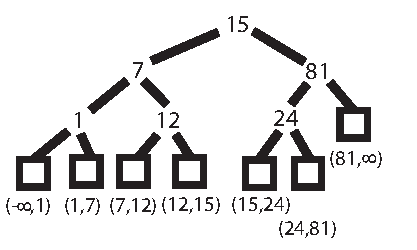
\includegraphics{pics/bvs}
\caption{Příklad binárního vyhledávacího stromu}
\label{fig.bvs.example}
\end{figure}

\end{priklad}

\begin{pozn}
V listech máme jen intervaly, každý vrchol implicitně určuje tyto
intervaly. (viz obr.~\ref{fig.bvs.example}) Tato vazba je jednotlivými
operacemi udržována.
\end{pozn}

\subsection{Algoritmus MEMBER}

\begin{algorithm}[!htb]
\caption{MEMBER pro binární vyhledávací stromy}
\label{alg:btr.mem}
\begin{algorithmic}
\STATE $t \leftarrow$ kořen
\WHILE {$t$ \text{není list a zároveň} $t$ \text{nereprezentuje} $x$} 
\IF {$x >$ \text{prvek reprezentovaný} $t$}
  \STATE $t \leftarrow$ pravý syn
\ELSE 
   \STATE $t \leftarrow$ levý syn $t$
\ENDIF
\ENDWHILE
\end{algorithmic}
\end{algorithm}


\subsection{Algoritmus INSERT}

\mnote{tohle je pouze pokus o alg. 
XXX dopsat podle nějakého důvěryhodného zdroje !}
\begin{enumerate}
  \item najdi list kam patří $x$ ($x_{i-1} < x < x_i$)
  \item udělej z něj vnitřní vrchol s hodnotou $x$
  \item přidej mu dva syny s intervaly $<x_{i-1}, x> , <x, x_i>$
  \item uprav strukturální podmínku na strom
\end{enumerate}


\subsection{Algoritmus DELETE}

DELETE(x) provedeme následovně: 

\begin{enumerate}
  \item nalezneme $x$ (vrchol reprezentující $x$)
  \item pokud jeden jeho syn je list, pak odstraníme vrchol + syna, který je
    list, druhý syn nahradí odstraněný vrchol
\mnote{co když oba synové jsou listy ?}
  \item pokud žádný jeho syn není list, pak:
    nalezneme vrchol $u$, reprezentující nejmenší prvek v $S$ větší než $x$.
    levý syn tohoto vrcholu je list.
    přemístíme prvek reprezentovaný tímto vrcholem do vrcholu
    reprezentujícího $x$ odstraníme $u$ a jeho levého syna, pravého syna
    $u$ dáme na místo $u$.
\end{enumerate}

Jak nalezneme vrchol reprezentující nejmenší prvek v $S$ větší než $x$ ?
Jsme ve vrcholu $t$ reprezentujícím $x$ a hledáme vrchol $u$:
\begin{algorithmic}
\STATE $u \leftarrow$ pravý syn $t$
\WHILE {\text{levý syn} $u \neq list$}
   \STATE $u \leftarrow$ levý syn $u$
\ENDWHILE
\end{algorithmic}

Čas pro operace MEMBER, INSERT a DELETE v binárním vyhledávacím stromě je
\\
$O(\text{délka stromu}) = O(\text{výška stromu})$.

% --------------------------------------------------------------------------
\section{Optimální binární vyhledávací stromy}

Budeme chtít reprezentaci binárního vyhledávacího stromu takovou, že 
bude optimalizovaná vzhledem k operaci MEMBER za předpokladu, že známe
pravděpodobnost provedení této operace na jednotlivé vrcholy stromu.

\subsection{Co je to optimální binární vyhledávací strom}

Prvky jsou uloženy ve vnitřních vrcholech stromu. 
Listy jsou intervaly $(-\infty, x_1)$, $(x_1, x_2)$, 
$\ldots$, $(x_n, \infty)$. Listy nemusíme implicitně
ve stromě zaznamenávat.
U optimálních stromů dále předpokládáme, že známe pravděpodobnosti 
operací $Access(x)$. 

\subsection{Algoritmus konstrukce}

Dána množina $S = \{x_1 < x_2 < ... < x_n \}$, provádí se pouze operace
MEMBER(x) a jsou dány pravděpodobnosti 
$\alpha_1, ..., \alpha_n, \beta_0, ..., \beta_n$, kde 
\begin{itemize}
\mnote{P značí pravděpodobnost}
\item $\alpha_i = P($prováděla se operace $MEMBER(x_i))$
\item $\beta_i = P($prováděla se operace $MEMBER(x)$ pro 
   $x \in <x_i, x_{i+1}>)$
\end{itemize}

kde $x_0 = - \infty, x_{n+1} = \infty$.
\par
Tedy jsou dány pravděpodobnosti přístupu k vnitřním vrcholům a k listům.
\par

Chceme nalézt binární vyhledávací strom reprezentující $S$ takový, že
operace MEMBER má nejmenší očekávaný čas.
\par
Očekávaný čas operace MEMBER je $\sum_{i=1}^{n} \alpha_i(a_i + 1) +
\sum_{i=0}^{n} \beta_i b_i$, kde 
\mnote{očekávaná hodnota = střední hodnota náhodné veličiny; n.v. s
diskrétním rozdělením má stř. hodnotu $\sum x_i p_i$}
$a_i$ je hloubka prvku reprezentujícího prvek $x_i$, $b_i$ je hloubka
listu reprezentujícího interval $<x_i, x_{i+1}>$.
\par

\subsubsection{Zobecníme úlohu:}

\mnote{XXX sjednotit indexy a závorky - buď $c(i,j)$ nebo $c_{i,j}$}
Dána množina $S = \{x_1 < x_2 < ... < x_n \}$ a ohodnocení $\alpha_i$ prvku
$x_i$ a $\beta_i$ intervalu $(x_i,x_{i+1})$.
Chceme zkonstruovat binární vyhledávací strom T reprezentující S takový,
že $hod(T)= \sum_{i=1}^{n} \alpha_i(a_i + 1) + \sum_{i=0}^{n} \beta_i b_i$
je minimální. \\
T je pak optimální binární vyhledávací strom.
Pro $1 \leq i \leq j \leq n$, $U_{i,j}$ je úloha nalézt optimální binární
vyhledávací strom pro $S_{i,j} = {x_i < x_{i+1} < ... < x_j}$ a hodnoty 
$\alpha_i, \alpha_{i+1}, ..., \alpha_j, \beta_{i-1}, \beta_i, ..., \beta_j$.

\par
\begin{pozorov}
\label{obvs-poz1}
% Pozorování 1: 
Nechť T je strom reprezentující množinu $S_{i,j}$ a kořen T
hodnotí prvek $x_k$ pro $i \leq k \leq j$. Nechť $T_l$ je podstrom levého
syna kořene, $T_p$ je podstrom pravého syna kořene. Pak: \\
$hod(T) = hot(T_l) + hod(T_p) + \sum_{l=i}^{j} \alpha_l + \sum_{l=i-1}^{j}
\beta_l$ \\
$T_l$ reprezentuje množinu $S_{i,k-1}$ a $T_p$ reprezentuje množinu $S_{k+1,j}$.
\end{pozorov}

\par
\begin{pozorov}
% Pozorování 2: 
Nechť platí předpoklady pozorování
% Pozorování 1 
\ref{obvs-poz1}
a nechť T je optimální
binární vyhledávací strom pro $S_{i,j}$. Pak $T_l$ je optimální
binární vyhledávací strom pro $S_{i,k-1}$ a $T_p$ je optimální
binární vyhledávací strom pro $S_{k+1,j}$.
\end{pozorov}

\par
\begin{pozorov}
% Pozorování 3: 
Když známe $hod(T_{k,k'})$ pro opt. bin. vyhl. strom
reprezentující množinu $S_{k,k'}$ kde $i \leq k \leq k' \leq j$ a $k'-k <
j-i$, pak $hod(T_{i,j})$ pro opt. bin. vyhl. strom je \\
$$
\sum_{l=i}^{j} \alpha_l + \sum_{l=i-1}^{j} \beta_l + min\{hod(T_{i,k-1}) +
hod(T_{k+1,j}), i \leq k \leq j\}
$$
Když 
$$
hod(T_{i,k-1}) + hod(T_{k+1,j})
\leq min\{hod(T_{i,k'-1}) + hod(T_{k'+1,j}), i \leq k' \leq j\}
$$
pak $\exists$ opt. bin. vyhl. strom pro $S_{i,j}$,
jehož kořen reprezentuje $x_k$.
\end{pozorov}

\par
Systematicky spočítáme $w_{i,j} = \sum_{l=i}^{j} \alpha_l + \sum_{l=i-1}^{j}
\beta_l$ pro všechny $1 \leq i \leq j \leq n$. Inicializujeme matice H,K
typu $n x n, H = K = 0$.
\mnote{XXX typu n krat n}

\begin{algorithmic}
\FOR {i=1,2,...,n} 
  \STATE $H_{i,i} = w_{i,i}, K_{i,i} = i$
\ENDFOR
\end{algorithmic}

$H_{i,j}$ pro $i \leq j$ bude $H_{i,j} = hod(T_{i,j})$ pro opt. bin. vyhl.
strom reprezentující $S_{i,j}$ a $K_{i,j}$ bude index prvku
reprezentovaného v kořeni $T_{i,j}$.

\begin{algorithm}[!htb]
\caption{Výpočet matic H, K}
\label{alg:obvs.puv}
\begin{algorithmic}
\FOR {every $i=1,2,..,n$}
  \STATE $H_{i,i} = w_{i,i}, K_{i,i} = i$
\ENDFOR
\STATE $j = 1$
\WHILE {$j < n$}
  \STATE $i = 1$
  \WHILE {$i+j \leq n$}
    \STATE $m = i, hod = H_{i+1,j}$ (1)
    \STATE $k = i+1$  (2)
    \WHILE {$k \leq i+j$ (3)} 
      \IF {$hod > H_{i,k-1} + H_{k+1,i+j}$}
        \STATE $hod = H_{i,k-1}+H_{k+1,i+j}$
	\STATE $m = k$
      \ENDIF
      \STATE $k = k + 1$
    \ENDWHILE
    \STATE $H_{i,i+j} = hod + w_{i,i+j}, K_{i,i+j} = m, i = i + 1$
  \ENDWHILE
  \STATE $j = j + 1$
\ENDWHILE
\end{algorithmic}
\end{algorithm}

\begin{theorem}
Uvedený algoritmus \ref{alg:obvs.puv} spočítá korektně matice $H$ a $K$ 
v čase $O(n^3)$ a vyžaduje $O(n^2)$ paměti.
\end{theorem}

$K_{i,j} \leq K_{i,j+1} \leq K_{i+1,j+1}$

\mnote{XXX obr. matice}

\subsubsection{Konstrukce opt. bin. vyhl, stromu ze znalosti matice $K$}
\begin{itemize}
\item kořen stromu bude $x_{K(1,n)}$.
\item podstrom levého syna bude optim. strom pro $S_{1,K(1,n)-1}$
\item podstrom pravého syna bude optim. strom pro $S_{K(1,n)+1,n}$
\end{itemize}

To nám dává rekurzivní algoritmus pro výstavbu opt. bin. vyhl. stromu z
matice $K$, strom takto zkonstruujeme v čase $O(n)$.


% --------------------------------------
\subsection{Snížení složitosti z kubické na kvadratickou}

XXX sloučit s částí předch subsekce

Chceme snížit ryhchlost konstrukce opt. bin. vyhl. stromu z kubické na
kvadratickou. Pro tento úkol použijeme \emph{kvadratické programování}. 
Pomocí této techniky lze modifikovat algoritmus pro konstrukci optimální
BVS tak, že bude mít místo složitosti $O(n^3)$ složitost $O(n^2)$.

Algoritmus~\ref{alg:obvs.puv} pro výpočet $H$ a $K$ jsme modifikovali tak,
že řádky (1),(2),(3) jsme nahradili řádky (1'),(2'),(3'). Tím vznikl
algoritmus~\ref{alg:obvs.modif}.

\begin{algorithm}[!htb]
\caption{Modifikovaný algoritmus pro výpočet matic H, K}
\label{alg:obvs.modif}
\begin{algorithmic}
\FOR {every $i=1,2,..,n$}
  \STATE $H_{i,i} = w_{i,i}, K_{i,i} = i$
\ENDFOR
\STATE $j = 1$
\WHILE {$j < n$}
  \STATE $i = 1$
  \WHILE {$i+j \leq n$}
    \STATE $m = K_{i,i} + j, hod = H_{i,m-1} + H_{m+i,i+j}$ (1')
    \STATE $k = K_{i,i+j} + 1$ (2') 
    \WHILE {$k \leq K_{i+1,j+1}$ (3')} 
      \IF {$hod > H_{i,k-1} + H_{k+1,i+j}$}
        \STATE $hod = H_{i,k-1}+H_{k+1,i+j}$
	\STATE $m = k$
      \ENDIF
      \STATE $k = k + 1$
    \ENDWHILE
    \STATE $H_{i,i+j} = hod + w_{i,i+j}, K_{i,i+j} = m, i = i + 1$
  \ENDWHILE
  \STATE $j = j + 1$
\ENDWHILE
\end{algorithmic}
\end{algorithm}

Modifikovaný algoritmus: Třetí vnořený cyklus vyžaduje čas 
$O(K_{i+1,j+1} - K_{i,j})$. Tedy druhý vnořený cyklus vyžaduje čas 
$O(K_{2,2+j} - K_{1,1+j} + K_{3,3+j} - K_{2,2+j} + K_{4,4+j} - K_{3,3+j} +
... + K_{n-j,n} - K_{n-j-1,n-1}) = O(K_{n-j,n}) = O(n)$.

\begin{theorem}
Za předpokladu $K_{i,j} \leq K_{i,j+1} \leq K_{i+1,j+1}$ pro každé 
$1 \leq i \leq j \leq n - 1$ modifikovaný algoritmus korektně spočítá
matice $H$ a $K$ v čase $O(n^2)$ a vyžaduje paměť $O(n^2)$.
\end{theorem}



\par
Vstup: dána čísla $w(i,j), 1 \leq i \leq j \leq n$\\
Výstup: definujeme  $c(i,j) = $
 \(
 \begin{cases}
 	0
		&\text{pro } i=j, \text{kde } i = 1,2,..., n\\
	w(i,j) + min\{c(i,k-1) + c(k,j),
		i < k \leq j\}&\text{pro } i \neq j
 \end{cases}
 \)

Úkolem je tedy nalézt čísla $c(i,j)$.
Čísla $c(i,j)$ budou tvořit výstup algoritmu. Když použijeme modifikaci
algoritmu pro hledání opt. bin. vyhl. stromu, pak spočítáme $c(i,j)$ v
čase $O(n^3)$.
\par

\begin{defn}
$K(i,j) = min\{l, l=i+1, ..., j \text{ a platí }
c(i,l-1) + c(l,j) \leq c(i,k-1) + c(k,j) \forall k = i+1, ...,j\}$ 
\end{defn}

Když $K(i,j) \leq K(i,j+1) \leq K(i+1,j+1)$ pro $i \leq j$, pak lze použít
algoritmus vyžadující čas $O(n^2)$. (tj. můžeme použít rychlejší
modifikaci algoritmu pro hledání opt. bin. vyhl. stromu a
spočítáme $c(i,j)$ v čase $O(n^2)$)

\begin{pozn}
Vztah kvadratického programování a hledání opt. bin. vyhl. stromu:
Položme $w(i,j) = \sum_{l=i}^{j} \alpha_l + \sum_{l=i-1}^{j} \beta_l$, pak
$c(i,j) = H_{i+1,j}$.
\end{pozn}

\par
Chceme ukázat, že když platí

\begin{itemize}
\item (A) $w(i,j) \leq w(i',j')$ pro $i' \leq i \leq j \ leq j'$ 
\item (B) $w(i,j) + w(i',j') \leq w(i,j') + w(i',j)$ pro 
$i \leq i' \leq j \ leq j'$ 
\end{itemize}

pak platí 
$K(i,j) \leq K(i,j+1) \leq K(i+1,j+1)$ pro $1 \leq i \leq j$.

\begin{lemma}
Za uvedených předpokladů platí \\
$c(i,j) + c(i',j') \leq c(i,j') + c(i',j)$ pro $i \leq i' \leq j \ \leq j'$ 
\end{lemma}

\begin{proof}
indukcí dle $j'-i$: \\
platí: když $i = i'$ nebo $j = j'$, pak triviálně platí \\
$c(i,j) + c(i',j') \leq c(i,j') + c(i',j)$ 

iniciální krok: když $j'-i \leq 0$, pak platí buď $i = i'$ nebo $j = j'$. \\
indukční krok: předpokládejme, že nerovnost platí, když $j'-i < n$ a
nechť $j'-i = n$, kde $n \geq 2$.

\begin{enumerate}
% 1)
\item $j = i'$ pak máme dokázat, že \\
$c(i,j) + c(j,j') \leq c(i,j')$. označme $K(i,j') = l$.

\begin{enumerate}
\item
(1a)
$l \leq j$ pak $c(i,j) + c(j,j') \stackrel{\text{z def } c(i,j)}{\leq} w(i,j) + c(i,l-1) + c(l,j)+ c(j,j')
\stackrel{\text{z (A) a ind. předp.}}{\leq} w(i,j') + c(i,l-1) = c(i,j)$  \\
víme, že $i < l \leq j$, tedy $j'-l < j'-i$. \\
$\Rightarrow$ (1a) platí.
\item
(1b) $l \geq j$, důkaz stejný jako pro 1a. \\
$\Rightarrow$ 1 platí.
\end{enumerate}

% 2)
\item $j > j'$ \\
označme $k = K(i,j'), l = K(i',j)$ \\

\begin{enumerate}
\item (2a) $l \leq k$, pak $i' < l < \leq j, i < k < j \leq j'$ \\
\begin{align*}
&c(i,j) + c(i',j') \\
\leq &w(i,j) + c(i,l-1) + c(l,j) + w(i',j') + c(i',k-1) + c(k,j') \\
= &w(i,j) + w(i',j') + c(i,l-1) + c(i',k-1) + c(l,j) + c(k,j') \\
\stackrel{\text{podle (B)}}{\leq} 
&w(i,j') + w(i',j) + c(i,k-1) + c(i',l-1) + c(l,j) + c(k,j') =
\end{align*}
\mnote{$c(i,k-1) + c(i',l-1)$ jsme dostali z ind. předp.}

víme, že $i \leq i' \leq l-1 \leq k-1$ a $k-1-i < j'-i$. \\
Potom 

\begin{align*}
= &w(i,j') + c(i,k-1) + c(k,j') + w(i',j) + c(i,l-1) c(l,j) \\
= &c(i,j') + c(i',j)
\end{align*}

\item (2b) $k \leq l$ důkaz je analogický jako pro (2a).
\end{enumerate}
$\Rightarrow$ 2 platí.
\end{enumerate}
$\Rightarrow$ lemma je dokázané.
\end{proof}

\begin{lemma}
Když $c(i,j) + c(i',j') \leq c(i,j') + c(i',j)$ pro $i \leq i' \leq j \leq
j'$, pak platí \\
$K(i,j) \leq K(i,j+1) \leq K(i+1,j+1)$
\end{lemma}

\begin{proof}
Ukážeme, že platí $K(i,j) \leq K(i,j+1)$, důkaz druhé nerovnosti je
analogický. \\
Abychom dokázali $(i,j) \leq K(i,j+1)$, tak stačí ukázat, že platí \\
$c(i,k-1) + c(k,j) <  c(i,k'-1) + c(k',j)$ pak
$c(i,k-1) + c(k,j+1) <  c(i,k'-1) + c(k',j+1)$ pro $i < k' < k \leq j$.

požadovaná nerovnost plyne z této nerovnosti: \\
\begin{align*}
&c(i,k'-1) + c(k',j) - c(i,k-1) - c(k,j) \\
\stackrel{c(i,k'-1) > 0}{\leq} 
&c(i,k'-1) + c(k',j+1) - c(i,k-1) - c(k,j+1)
\end{align*}

skončili jsme s triky, upravíme nerovnost a vyjde to: \\
\begin{align*}
&c(i,k'-1) + c(k',j) + c(i,k-1) + c(k,j+1) \\
\leq &c(i,k'-1) + c(k',j+1) + c(i,k-1) + c(k',j+1) 
\end{align*}

$c(k',j) + c(k,j+1) \leq c(k',j+1) + c(k,j)$
platí $k' < k \leq j \leq j+1$ ... nerovnost platí dle předpokladu
(položíme i = k', i'=k, j=j, j'=j+1)
\mnote{XXX pokud se divíte $j=j$, nedivte se, znamená to, že j z 1. části se
rovná j z druhé části :) chce to lepší značení}
\end{proof}


% --------------------------------------------------------------------------
\section{Skorooptimální binární vyhledávací stromy}

% Jenom že existují, lineární konstrukce. Aha --- viz cvičení.

% \mnote{referát by Ladislav Strojil}
\newtheorem{fakt}{Fakt}

\renewcommand{\labelenumi}{\arabic{enumi})}
\newcommand{\oops}[1]{\textbf{#1}}

% tady jsem z referatu vytrhnul definici bin. opt. vyhr. stromu a presunul
% ji nahoru k bin. opt. vyhl. stromum
% V. Kotal, 2004

\begin{defn} Nechť $S=\{x_1 < x_2 < \ldots < x_n\}$ 
a nechť $\beta_i$ (resp. $\alpha_j$) je prav\-dě\-po\-dob\-nost operace 
$Access(a,S)$, kde $a=x_i$ (resp. $x_j < a < x_{j+1}$) pro $1 \leq i \leq n$ 
(resp. $0 \leq j \leq n$).
Potom $\beta_i\geq0$, $\alpha_i\geq0$ a $\sum{\beta_i}+\sum{\alpha_i}=1$. 
(2n+1)-tice $(\alpha_0,\beta_1,\alpha_1,\ldots,\beta_n,\alpha_n)$ se nazývá 
\emph{rozdělení (pravděpodobnosti) přístupu}.
\end{defn}

Strom potom konstruujeme rekurzí tak, aby \emph{průměrná vážená cesta} 
ve stro\-mě byla co nejkratší.
\par

Takový strom lze konstruovat pomocí rekurzivního výpočtu zkoušením všech 
kandidátů na kořen. To lze v čase $O(n^2)$, protože volba kořene jednoznačně určuje 
prvky pravého i levého podstromu (neboť se jedná o vyhledávací strom).
Takový strom lze konstruovat pomocí rekurzivního výpočtu zkoušením všech 
kandidátů na kořen. To lze v čase $O(n^2)$, protože volba kořene jednoznačně určuje 
prvky pravého i levého podstromu (neboť se jedná o vyhledávací strom).
\subsection{Aproximace optimálních stromů}

\par
Při konstrukci se budeme snažit volbou kořene podstromu rozdělit prvky na dvě stejně pravděpodobné množiny.

Uvažujme následující situaci. $S=\{x_1, x_2, x_3, x_4\}$ s pravděpodobnostmi pří\-stu\-pu
($\alpha_0$, $\beta_1$, $\alpha_1$, $\beta_2$, $\alpha_2$, $\beta_3$, $\alpha_3$, $\beta_4$, $\alpha_4$) = 
$(\frac{1}{6},\frac{1}{24},0,\frac{ 1}{8},0,\frac{ 1}{8},\frac{ 1}{8}, 0,\frac{ 5}{12})$.

\par
Doporučuji si představit uvedené body na reálné ose tak, že $\alpha_0$ je v bodě $0$, $\alpha_4$ v bodě $1$.

\par
Bod $\frac{1}{2}$ padne buď do $\beta_i$ nebo do $\alpha_j$ pro nějaké $i$, resp. $j$. V prvním případě zvolíme $x_i$ jako 
kořen stromu, jinak volíme mezi $x_j$ a $x_{j+1}$, podle toho, zda $\frac{1}{2}$ leží v levé nebo pravé polovině $\alpha_j$. 

\par
V našem případě volíme $x_3$ jako kořen stromu.

\par
Pro rozhodnutí o kořenu levého podstromu vrchol, který popsaným způ\-sobem odpovídá bodu $\frac{1}{4}$. Tento postup není totožný s postupem, 
kdy se bere bod $\frac{1}{2}$ v 
nově vzniklé podúloze, protože při konstrukci podstromu bychom zanedbali část intervalu $\alpha_3$.

\subsection{Podrobnější popis naznačené metody}

Nechť 
\begin{equation} 
s_0 = \frac{\alpha_0}{2} \\ s_i = s_{i-1} + \frac{\alpha_{i-1}}{2} + \beta_i + \frac{\alpha_i}{2}.
\end{equation}

\par
Uvědomte si, že $s_i$ jsou středy intervalů příslušejících "neúspěšnému
vy\-hle\-dá\-vá\-ní", tj. $(x_i,x_{i+1})$.

\par
Volání funkce $construct\_tree(0,n,0,1)$ vytvoří skoro optimální
vyhledávací strom dle popsané metody.

\ \newline
\oops{procedure} contruct\_tree(i,j,cut,l)

\emph{Poznámka: Předpokládáme, že parametry volané funkce splňují následující podmínky.}
\begin{enumerate}
\item $i$ a $j$ jsou celá čísla taková, že $0 \leq i < j \leq n$
\item $l$ je celé číslo, $l \geq 0$
\item $cut=\sum_{p=1}^{l-1}{x_p 2^{-p}}$, kde $x_p \in \{0, 1\}$ pro všechna $p$
\item $cut \leq s_i \leq s_j \leq cut + 2^{-l+1}$
\end{enumerate}
\emph{Volání $construct\_tree(i,j,,)$ vytvoří binární vyhledávací strom pro vrcholy $i+1, \ldots, j$ a listy $i, \ldots, j$.}

\oops{begin}

\ \ \ \oops{if} $i+1=j$ (případ A) \oops{return} kořen=j, levý list=i, pravý list=j;

\ \ \ \ \ \oops{else}

\ \ \ \ \ \ \ \ najdi k takové, že

\ \ \ \ \ \ \ \ 5) $i < k \leq j$

\ \ \ \ \ \ \ \ 6) $k = i + 1$ nebo $s_{k-1} \leq cut + 2^{-l}$

\ \ \ \ \ \ \ \ 7) $k = j$ nebo $s_{k} \geq cut + 2^{-l}$

\ \ \ \ \ \ \ \ \emph{Takové $k$ vždy existuje, protože parametry funkce splňují podmínku 4.}

\ \ \ \ \ \ \ \ \oops{if} $k = i + 1$ (případ B) \oops{return}

\ \ \ \ \ \ \ \ \ \ \ \ \ \ \ \ \ \ \ \ \ \ \ \ kořen=i+1

\ \ \ \ \ \ \ \ \ \ \ \ \ \ \ \ \ \ \ \ \ \ \ \ levý list=i

\ \ \ \ \ \ \ \ \ \ \ \ \ \ \ \ \ \ \ \ \ \ \ \ pravý list=\oops{construct\_tree}(i+1,j,cut+$2^{-l}$,l+1);

\ \ \ \ \ \ \ \ \oops{if} $k = j$ (případ C) \oops{return} 

\ \ \ \ \ \ \ \ \ \ \ \ \ \ \ \ \ \ \ \ \ \ \ \ kořen=j

\ \ \ \ \ \ \ \ \ \ \ \ \ \ \ \ \ \ \ \ \ \ \ \ levý list=\oops{construct\_tree}(i,j-1,cut,l+1)
	
\ \ \ \ \ \ \ \ \ \ \ \ \ \ \ \ \ \ \ \ \ \ \ \ pravý list=j;

\ \ \ \ \ \ \ \ \oops{if} $i + 1 < k < j$ (případ D) \oops{return}

\ \ \ \ \ \ \ \ \ \ \ \ \ \ \ \ \ \ \ \ \ \ \ \ kořen=k

\ \ \ \ \ \ \ \ \ \ \ \ \ \ \ \ \ \ \ \ \ \ \ \ levý list=\oops{construct\_tree}(i,k-1,cut,l+1)
	
\ \ \ \ \ \ \ \ \ \ \ \ \ \ \ \ \ \ \ \ \ \ \ \ pravý list=\oops{construct\_tree}(k,j,cut+$2^{-l}$,l+1);

\oops{end}


\begin{theorem}
Nechť $b_i$ je hloubka vrcholu $x_i$ a $a_j$ je hloubka listu $(x_j,x_{j+1})$ ve stromě $T_{BB}$ vytvořeném funkcí 
\oops{construct\_tree}(0,n,0,1). Potom

$b_i \leq \lfloor \log{1/\beta_i}\rfloor$, $a_j \leq \lfloor \log{1/\alpha_j}\rfloor + 2$ 
\end{theorem}

\begin{proof}
\emph{Věta říká, že hloubka vrcholu roste s klesající pravděpodobností přístupu k tomuto vrcholu.}

Plyne z následujících faktů.
\end{proof}

\begin{fakt}
Jestliže hodnoty parametrů funkce \oops{construct\_tree} splňují 
podmínky 1-4 a $i + 1 \neq j$, potom k splňující požadované podmínky existuje 
a hodnoty parametrů rekurzivních volání \oops{construct\_tree} splňuji 1-4.
\end{fakt}

\begin{proof} 
\ \par
Předpokládejme, že parametry splňují 1 -- 4 a $i + 1 \neq j$. 
Potom zřejmě platí $cut \leq s_j \leq cut + 2^{-l+1}$. Pro spor předpokládejme, 
že neexistuje neexistuje žádné $k$, $i < k \leq j$, pro které 
by platilo $s_{k-1} \leq cut+2^{-l}$ a $s_{k} \geq cut+2^{-l}$. 

Potom ovšem buď pro všechna $k$ taková, že $i < k \leq j$, 
platí $s_{k} < cut+2^{-l}$ nebo 
pro všechna $k$ taková, že $i < k \leq j$, platí $s_{k-1} > cut+2^{-l}$.

\par
V prvním případě $k = j$ odpovídá požadovaným podmínkám, 
v druhém jim odpovídá $k = i + 1$. Tedy $k$ vždy existuje.

\par
Zbývá ukázat, že nové parametry volání funkce splňují požadované 
pod\-mín\-ky. To ale plyne z toho, že $k$ splňuje 5-7 a  $i+1 \neq j$.
\end{proof}

\begin{fakt}
Hodnoty parametrů všech volání \oops{construct\_tree} splňují podmínky 1-4.
\end{fakt}
\begin{proof} 
Indukcí. \oops{construct\_tree}(0, n, 0, 1) splňuje 1-4 a pomocí předchozího faktu.
\end{proof}

Řekneme, že vrchol $h$ (resp. list $h$) je vytvořen voláním 
\oops{construct\_tree}(i, j, cut, l), jestliže $h = j$ (resp. $h =j$ nebo $h = i$) a 
byl proveden případ A, nebo $h = i + 1$ (resp. $h = i$) a byl proveden případ B, 
nebo $h = j$ a byl proveden případ C, nebo  $h = k$ 
a byl proveden případ D.

\par
Dále něchť $b_i$ je hloubka vrcholu $i$ a $a_j$ hloubka listu $j$ ve 
stromě vráceném $construct\_tree(0,n,0,1)$.

\begin{fakt}
Je-li vrchol $h$ (resp. list $h$) vytvořen voláním 
$construct\_tree(i,j,cut,l)$, potom $b_h + 1 = l$ (resp. $a_h = l$).
\end{fakt}
\begin{proof}
Indukcí podle $l$. 
\end{proof}
\begin{fakt}
Je-li vrchol $h$ (resp. list $h$) vytvořen voláním 
$construct\_tree(i,j,cut,l)$, potom $\beta_h \leq 2^{-l+1}$ (resp. $\alpha_h \leq 2^{-l+2}$).
\end{fakt}
\begin{proof}
Parametry splňují 4 a tedy
$2^{l+1} \geq s_j - s_i = (\alpha_i + \alpha_j)/2 + \beta_{i+1} + \alpha_{i+1} + \ldots + \beta_j \geq \beta_h$ (resp. $\alpha_h/2$)
\end{proof}

\begin{proof}[věty]
Z faktů 3 a 4 obdržíme $\beta_h \leq 2^{-b_h}$ a $\alpha_h \leq 2^{-a_h+2}$. 
Zlogaritmováním a převedením na celočíselné hodnoty dostáváme tvrzení věty.
\end{proof}

\par
Věty 1 a 2 ukazují, že hloubka vrcholu je přibližně rovna logaritmu 
pře\-vrá\-ce\-né hodnoty prav\-dě\-po\-dob\-nosti přístupu k tomuto vrcholu.

\begin{defn}
Nechť $(\gamma_1,\gamma_2, \ldots, \gamma_n)$ je diskrétní rozdělení 
pravděpodobnosti. Potom se funkce 
$H(\gamma_1,\gamma_2, \ldots, \gamma_n) = - \sum_{i = 1}^{n}\gamma_i\log{\gamma_i}$ 
nazývá entropie rozdělení.
\end{defn}

\par
Povšimněte si, že entropie nezáleží na vytvořeném stromě, 
jenom na prav\-dě\-po\-dob\-nostech přístupu. 

\begin{theorem}
Nechť $P_{BB}$ je vážená délka cesty zkonstruovaného stromu. Potom

\begin{eqnarray} 
\nonumber P_{BB} \leq \sum{\beta_i} \lfloor\log{1/\beta_i}\rfloor + \sum{\alpha_j} \lfloor\log{1/\alpha_j}\rfloor + 1 + \sum{\alpha_j} \leq
\\ \leq H(\alpha_0,\beta_1,\alpha_1,\ldots,\beta_n,\alpha_n) + 1 + \sum{\alpha_j}
\end{eqnarray} 
\end{theorem}
Navíc
\begin{theorem}
Nechť $P_{BB}$ je vážená délka cesty zkonstruovaného stromu a nechť 
$P_{opt}$ je vážená délka cesty v optimálním stromu. ($B = \sum\beta_i$) 
Potom 
\begin{enumerate}
\item $\max\{\frac{H-dB}{\log{(2+2^{-d})}}; d \in \mathbf{R}\} \leq P_{opt} \leq P_{BB} \leq H + 1 + \sum{\alpha_j}$
\item $P_{BB} \leq P_{opt} + B(\log e + \log(P_{opt}/B)) + 2\sum{\alpha_j}$
\end{enumerate}

\end{theorem}
\begin{proof}
Plyne z věty 5 (původní číslování, viz \cite{mehlhorn}, strana 175) a věty 2.
\end{proof}

Je to jenom složité počítání, jde o to, že dovedeme odhadnout, 
jak velká dovede být ta vážená cesta v námi vytvořeném stromě.

$P_{BB} - P_{opt} \leq \log P_{opt}$, což je přibližně $log H$.

\subsection{Časová složitost}

Pro sestrojení stromu s jedním vrcholem potřebuje metoda konstatní čas, tj. $T(1)=c_1$.

Pro $n > 1$ je potřeba najít $k$ a dojde až ke dvěma rekurzivním 
voláním \oops{construct\_tree}.
Nechť $T(m,n)$ je čas potřebný pro nalezení $k$, kde $m = k - i$ 
(tj. vzdálenost k od počátku zkoumaného úseku).
\oops{construct\_tree} je voláno maximálně dvakrát, v případě D první 
volání sestrojí strom s $k - 1 - i = m - 1$ 
vrcholy a druhé volání strom s $j - k = n - m$.

Tedy $T(n) \leq \max(T(m-1) + T(n-m) + T_S(n,m) + c_2)$.

Zde $c_2$ je konstanta měřící složitost předávání parametrů.

Dodefinujeme-li $T(0) = 0$, potom uvedená nerovnost platí i pro případy 
B a C. Zavedeme-li dále konvenci $T_S(1,m) = 0$ a 
$c = max(c_1, c_2)$, dotáváme zjednodušený výraz:

\begin{equation} 
T(0) = 0 \\
T(n) \leq \max_{1 \leq m < n}(T(m-1) + T(n-m) + T_S(n,m) + c)
\end{equation} 


\subsection{Hledání $k$}

Číslo $k$ můžeme hledat binárním vyhledáváním (půlení intervalu), 
ale výsledná časová složitost by byla $O(n\log n)$

Principiální problém s vyhledáváním pomocí půlení intervalu je, 
že nám nalezení $k$ trvá dlouho i v případě, že je blízko
$i$ nebo $j$ a tedy neredukuje velikost podúlohy podstatným způsobem.

Řešením je kombinace exponenciálního a binárního vyhledávání. 
Tím do\-sáh\-ne\-me toho, že $k$, která jsou blízko krajním 
bodům intervalu, nalezneme rychleji.

Budeme vyhledávat od konců intervalu, ale ne v konstatních krocících.

$1)$ Porovnáme $s_r$ s $cut + 2^{-l}$, kde $r = \lfloor(i + 1 + j) / 2\rfloor$. 
Je-li $s_r \geq cut + 2^{-l}$, potom $k \in \{i + 1, \ldots, r\}$. 
Je-li $s_r \leq cut + 2^{-l}$, potom $k \in \{r, \ldots, j\}$. 
V dalším budeme předpokládat, že $k \in \{i + 1, \ldots, r\}$. 

Tento krok trvá konstantní čas.

$2)$ Nalezneme nejmenší $t$, $t = 0, 1, 2, \ldots$, takové, že $s_{i+2^t} \geq cut + 2^{-l}$.
Nazvěme jej $t_0$. $t_0$ lze nalézt v čase $d_2(t_0 + 1)$ pro nějakou konstantu $d_2$.

Potom $i + 2^{t_0-1} < k \leq i + 2^{t_0}$, tj. $2^{t_0} \geq k - i = m > 2^{t_0-1}$ a odtud $\log m > t_0 - 1$. 
Tedy trvání kroku 2 je omezené $d_2(2 + \log m)$.

$3)$ Binárním vyhledáváním na intervalu 
$i + 2^{t_0-1} + 1, \ldots, i + 2^{t_0}$ zjistíme přesnou hodnotu $k$.

Tohle zabere $d_3(\log(2^{t_0} - 2^{t_0-1}) + 1) = d_3 t_0 < d_3(1 + \log m)$ 
(pro nějakou konstantu $d_3$).

Tedy pro $i < k \leq \lfloor(i + 1 + j) / 2\rfloor$ nalezneme $k$ 
v čase menším než $d_3(1 + \log m)$. Zde se $m = k -i$. Symetricky lze $k$
nalézt v čase $\leq d(1 + \log(n - m + 1))$, v případě, že $\lfloor(i + 1 + j) / 2\rfloor < k$.

Tedy $T_S(n,m) = d(1 + \log \min(m, n - m + 1))$

Dostáváme pro \oops{construct\_tree} následující rekurzivní vztah.
\begin{eqnarray} 
\nonumber && T(0) = 0  \\
\nonumber && T(n) = \max_{1 \leq m < n}(T(m-1) + T(n-m) + d(1 + \log \min(m, n - m + 1)) + c)
\end{eqnarray} 

\begin{theorem}
Je-li vyhledávání $k$ implementováno pomocí uvedené kombinace exponenciálního 
a binárního vyhledávání, potom $T(n) = O(n)$.
\end{theorem}

\begin{proof}
Indukcí podle $n$ ukážeme $T(n) \leq (2d + c)n - d\log(n + 1)$.

Pro $n=0$ vztah zřejmě platí.

Pro $n > 0$ máme 
\begin{equation} 
T(n) = \max_{1 \leq m < n}(T(m-1) + T(n-m) +  d(1 + \log \min(m, n - m + 1)) + d + c) 
\end{equation} 

Tedy podle symetrie výrazu v $m - 1$ a $n - m$ dostáváme:
\begin{equation} 
T(n) \leq \max_{1 \leq m < (n+1)/2}(T(m-1) + T(n-m) +  d\log m + d + c)
\end{equation} 

Podle indukčního předpokladu dostáváme
\begin{eqnarray} 
\nonumber T(n) & \leq & \max_{1 \leq m < (n+1)/2}((2d+c)(m-1+n-m)- \\ && -\ d(\log m + \log(n-m+1)) + d \log m + (d +c))
\end{eqnarray} 

Což se rovná
\begin{equation} 
(2d+c)n + \max_{1 \leq m < (n+1)/2}(-d(1 + \log m - m + 1))
\end{equation} 

Výraz v závorce je vždy menší než nula a je největší pro 
$m = (n + 1) / 2$. Tedy dostáváme následující nerovnost:
\begin{equation} 
T(n) \leq (2d+c)n - d(1 + \log(n+1)/2) = (2d+c)n - d\log(n+1) 
\end{equation} 
\end{proof}


% --------------------------------------------------------------------------
\section{AVL stromy}

Binární vyhledávací stromy jsou poměrně příjemné jednoduchou implementací
operací nad nimi, ale není přitom nijak omezena jejich hloubka. Může se
tedy stát, že strom může vypadat spíše jako seznam, a časová složitost
operací bude tedy lineární. Pokud bychom však chtěli, aby měl strom co
nejmenší výšku (vzdálenost listů od kořene by se mohla lišit maximálně o
jedničku), byly by operace INSERT a DELETE náročné. Rozumným
kopmromisem mohou být právě AVL-stromy.

AVL stromy jsou nazvané podle jmen jejich tvůrců ({\bf A}del'son-{\bf V}elskii 
a {\bf L}andis). Původní článek o AVL stromech lze nalézt v~\cite{AVL-trees}.
% Adison-Vesley-Landis. 

\begin{defn}
Nechť $v$ je vnitřní vrchol stromu T. Potom 
\begin{itemize}
  \item $l(v)$ je délka nejdelší cesty z $v$ do listu v podstromu 
  	levého syna $v$.
  \item $p(v)$ je délka nejdelší cesty z $v$ do listu v podstromu 
  	pravého syna $v$. 
\end{itemize}
Pokud takový podstrom neexistuje, položme $l(v)$ resp. $p(v)$ rovno $-1$.
Dále označme $b(v) = l(v) - p(v)$. Vrchol $v$ nazveme \emph{vyvážený}, 
jestliže $b(v)$ nabývá hodnot $-1$, $0$ nebo $1$.
\end{defn}

\begin{defn}
\label{avl:definice}
AVL strom je binární vyhledávací strom takový, že pro každý vnitřní vrchol
$v$ platí $l(v) - p(v) \in \{-1,0,1\}$.
\end{defn}

\begin{pozn}
AVL stromy jsou jen jednou z možností jak vyvažovat stromy. 
\emph{Dokonale vyvážené stromy} stanovují podmínku, že pro každý uzel ve
stromu platí, že \emph{počty} uzlů v levém a pravém podstromu tohoto 
uzlu se liší nejvýše o jedničku. AVL stromy tento požadavek zeslabují
tak, že vyžadují, aby se \emph{výšky} levého a pravého podstromu libovolného
vrcholu lišily nejvýše o jedničku\footnote{Platí, že každý dokonale
vyvážený strom je zároveň AVL stromem. Opačné tvrzení neplatí.}.
Úvod do vyvážených binárních stromů lze nalézt např. v~\cite{Topfer}.
\end{pozn}

\begin{theorem}
AVL-strom o $n$ vrcholech má výšku nejvýše $2 \log n$.
\end{theorem}

\begin{proof}
Označme $N(h)$ minimální počet vrcholů AVL stromu výšky $h$. Můžeme tedy
$N(h)$ definovat takto:
\begin{align*}
&N(0) = 1 \\
&N(1) = 2 \\
&N(h) = 1 + N(h-1) + N(h-2)
\end{align*}

Je zřejmé, že platí $N(h) \geq 2 N(h-2)$ nebo $N(h-2) \leq N(h-1)$. 

Odtud dostaneme, že $N(h) \geq 2^{h/2}$ a tedy
$h \leq 2 \log N(h)$. Nerovnost $N(h) \geq 2^{h/2}$ dokážeme indukcí:

\begin{enumerate}
  \item $N(0) = 1 \geq 2^{0/2} = 1$ \\
   	$N(1) = 2 \geq 2^{1/2}$
  \item $N(h) \geq 2 N(h-2) \geq 2 \cdot 2^{h/(2-1)} = 2^{h/2}$
\end{enumerate}

Všechny vrcholy AVL stromu jsou tedy vyvážené. Nevyvážené vrcholy mohou
vzniknout při operacích INSERT a DELETE. Při tom se může hodnota $b(v)$
změnit maximálně o jedničku. Hodnota $b(v)$ nevyváženého vrcholu bude tedy
$-2$ nebo $2$.
\end{proof}


\subsection{Algoritmus INSERT}

Vložení nového vrcholu do AVL-stromu se provádí stejně jako v
nevyvažovaných binárních vyhledávacích stromech. Při tom se však u
některých vrcholů může porušit podmínka na vyváženost. Mějme 
strom na obrázku~\ref{avltree}.

\begin{figure}[!htb]
\centering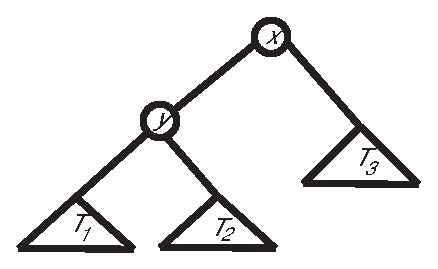
\includegraphics{pics/avl}
\caption{AVL strom}
\label{avltree}
\end{figure}

V tomto stromě jsou výšky podstromů $T_1$, $T_2$ a $T_3$ stejné. 
Pokud při vložení
nového vrcholu do podstromu T1 vzroste výška tohoto podstromu, bude vrchol
$x$ nevyvážený. Jeho vyvážení se však provede jednoduše pomocí 
tzv.~LL-rotace. (viz~obr.~\ref{avl-ll})

\begin{figure}[!htb]
\centering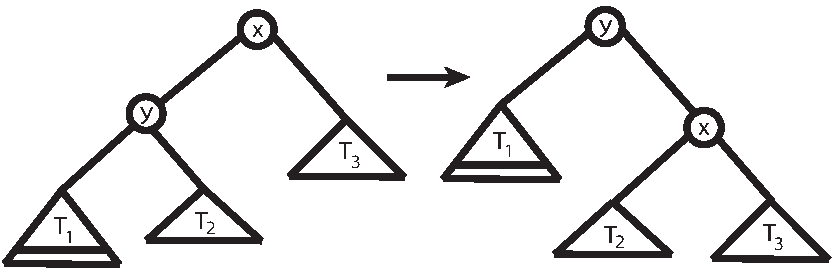
\includegraphics{pics/avl-ll}
\caption{LL-rotace pro AVL stromy}
\label{avl-ll}
\end{figure}

Pokud bychom však chtěli nový vrchol vložit do $T_2$ a výška tohoto podstromu
by vzrostla, byl by opět vrchol $x$ nevyvážený. To se může napravit pomocí
LR-rotace. (viz~obr.~\ref{avl-lr})

\begin{figure}[!htb]
\centering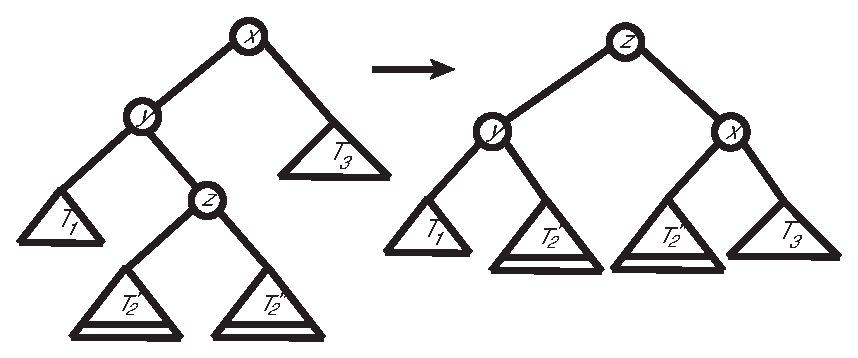
\includegraphics{pics/avl-lr}
\caption{LR-rotace pro AVL stromy}
\label{avl-lr}
\end{figure}

Poznamenejme, že na vyváženost nemá vliv, zda jsme vrchol vložili do
$T_{2}'$,
nebo do $T_{2}"$. Při vkládání nového vrcholu do pravého podstromu vrcholu
$x$ se pro vyvážení používají rotace RR-rotace a RL-rotace, které jsou 
symetrické k již uvedeným rotacím.

\begin{samepage}
LL-rotaci a RR-rotaci se také někdy říká jednoduchá rotace, kdežto
LR-rotaci a RL-rotaci se říká dvojitá rotace. Všimněte si, že po rotaci je
výška podstromu, se kterým se rotace prováděla, stejná jako jeho výška
před vložením nového vrcholu. Tedy po rotaci není narušena vyváženost
nějakého předka. Stačí tedy vyvážit ten nevyvážený vrchol, který je ve
stromu nejníže. Pokusme se nyní charakterizovat ten vrchol, který je třeba
vyvážit. Samozřejmě, že vrchol $x$ leží na cestě od kořene k přidanému
vrcholu a platí:
\begin{itemize}
\item buď $b(x)=1$ a nový vrchol je přidáván vlevo od $x$
\item nebo $b(x)=-1$ a nový vrchol je přidáván vpravo od $x$
\end{itemize}
\end{samepage}

Navíc pro každý vrchol $y$ na cestě od $x$ do přidaného listu je $b(y)=0$,
neboť jinak by byl sám nevyvážený, nebo by nezměnil svou výšku a tedy 
by nebylo třeba vyvažovat ani $x$.

Operace INSERT je formálně popsána algoritmem~\ref{alg:avl.ins}.

\begin{algorithm}[!htb]
\caption{INSERT pro AVL stromy}
\label{alg:avl.ins}
\begin{algorithmic}
\STATE INSERT($c$)
\STATE $r \leftarrow$ kořen
\WHILE {$r$ != NIL} 
\IF {$\text{prvek reprezentovaný } r = c$}
  \STATE END
\ENDIF
\IF {$balance(r)$ != $0$}
   \STATE $x := r$
\ENDIF
\IF {$\text{prvek reprezentovaný } r > c$}
  \STATE $r := left(r)$
\ELSE
  \STATE $r := right(r)$
\ENDIF
\ENDWHILE
\STATE \COMMENT {vložení nového vrcholu}
\STATE $r := \text{nový vrchol}$
\STATE $key(r):=c$
\STATE $b(r):=0$
\STATE $left(r):=nil$
\STATE $right(r):=nil$
\STATE $r:=x$
\STATE VYVAZUJ($r$)
\end{algorithmic}
\end{algorithm}


\begin{algorithm}[!htb]
\caption{VYVAZUJ pro AVL stromy}
\label{alg:avl.bal}
\begin{algorithmic}
\STATE \COMMENT {úprava balance (stačí od $x$ do vloženého listu)}
\WHILE {$r$ != NIL} 
  \IF {$\text{prvek reprezentovaný } r > c$}
        \STATE $balance(r) := balance(r) + 1$
        \STATE $r:=left(r)$
  \ENDIF
  \IF {$\text{prvek reprezentovaný } r < c$}
        \STATE $balance(r) := balance(r) - 1$
        \STATE $r := right(r)$
  \ELSE
        \STATE $r := NIL$
  \ENDIF
\ENDWHILE
\IF {$balance(x) = 2$}
  \IF {$\text{prvek reprezentovaný } left(x) > c$}
        \STATE LL-rotace
  \ELSE
        \STATE LR-rotace
  \ENDIF
\ENDIF
\IF {$balance(x) = -2$}
  \IF {$\text{prvek reprezentovaný } right(x) < c$}
        \STATE RR-rotace
  \ELSE
        \STATE RL-rotace
  \ENDIF
\ENDIF
\end{algorithmic}
\end{algorithm}



\subsection{Algoritmus DELETE}

Ubírání vrcholů z AVL-stromu se provádí stejně jako u nevyvážených
binárních vyhledávacích stromů. To znamená, že se ubíraný vrchol nahradí
nejpravějším vrcholem levého podstromu nebo nejlevějším vrcholem pravého
podstromu\footnote{To je klasický postup operace DELETE pro BVS popsaný
v~\cite{Topfer}, str.~70.}. 
Při tom se samozřejmě mohou také některé vrcholy stát
nevyváženými. To se opět řeší pomocí rotací.

\begin{algorithm}[!htb]
\caption{DELETE pro AVL stromy}
\label{alg:avl.del}
\begin{algorithmic}
\STATE DELETE($x$)
\STATE $r \leftarrow$ otec vrcholu reprezentovaného $x$
\STATE \COMMENT {vrcholu $left:=r$ jsme odebrali levého syna}
\WHILE {$r != NIL$}
\STATE \COMMENT {Prochází vrcholy od otce ubraného vrcholu ke kořeni}
  \IF {$left$}
        \IF {$b(r) = 0$}
		\STATE \COMMENT {Vrchol $r$ je stále vyvážený a výška jeho podstromu se nezměnila}
                \STATE $b(r) := -1$
        \ENDIF
        \IF {$b(r) = 1$}
		\STATE \COMMENT {Vrchol $r$ je stále vyvážený, ale výška jeho podstromu se snížila}
                \STATE $b(r) := 0$
	\STATE \COMMENT {Je třeba vyvažovat}
        \ELSE                            
                \STATE VYVAZUJ\_RIGHT(right($r$))
        \ENDIF
  \ELSE
        \IF {$b(r)=0$}
		\STATE \COMMENT {Vrchol $r$ je stále vyvážený a výška jeho podstromu se nezměnila}
                \STATE $b(r)=1$                  
                \STATE END
	\ENDIF
        \IF {$b(r)=-1$}
		\STATE \COMMENT {Vrchol $r$ je stále vyvážený, ale výška jeho podstromu se snížila}
                \STATE $b(r):=0$
		\STATE \COMMENT {Je třeba vyvažovat}
        \ELSE
		\STATE VYVAZUJ\_LEFT(left($r$))
        \ENDIF
  \ENDIF
\STATE $x:=r$
\STATE $r:=otec(r)$
\STATE $left:=left(r)=x$
\ENDWHILE
\end{algorithmic}
\end{algorithm}
%\end{samepage}

%\begin{samepage}
Operace DELETE je formálně popsána algoritmem~\ref{alg:avl.del}.
V algoritmu se používají dvě procedury pro vyvažování popsané v
algoritmech~\ref{alg:avl.del.vyvazuj.right}~a~\ref{alg:avl.del.vyvazuj.left}.

\begin{algorithm}[!htb]
\caption{VYVAZUJ\_RIGHT pro AVL stromy}
\label{alg:avl.del.vyvazuj.right}
\begin{algorithmic}
\STATE VYVAZUJ\_RIGHT(x)
\IF {$b(x) = 0$}
        \STATE RR-rotace
	\STATE END
\ENDIF        
		\STATE \COMMENT {Výška podstromu se nezměnila}
\IF {$b(x) = -1$}
        \STATE RR-rotace
\ELSE
        \STATE RL-rotace
\ENDIF
\end{algorithmic}
\end{algorithm}

\begin{algorithm}[!htb]
\caption{VYVAZUJ\_LEFT pro AVL stromy}
\label{alg:avl.del.vyvazuj.left}
\begin{algorithmic}
\STATE VYVAZUJ\_LEFT(x)
\IF {$b(x) = 0$}
        \STATE LL-rotace
		\STATE \COMMENT {Výška podstromu se nezměnila}
        \STATE END             
\ENDIF
\IF {$b(x) = 1$}
        \STATE LL-rotace
\ELSE
        \STATE LR-rotace
\ENDIF
\end{algorithmic}
\end{algorithm}
%\end{samepage}


%\begin{samepage}
Problém je, že ne při všech rotacích se zachovává výška podstromu, jak
tomu bylo u operace INSERT. Proto se zde vyvažování neomezí pouze na jeden
vrchol. Při operaci DELETE se může provést až $\log n$ rotací. Každopádně
složitost operace DELETE je stejně jako složitost operace INSERT $O(\log n)$.
\mnote{XXX dokázat max. počet rotací při DELETE}

% tohle by melo flushnout floats
% dalsi varianta:
% ctan macro/latex/contrib/supported/ placeins.sty 
% \floatbarrier command 
%\clearpage
\FloatBarrier

% --------------------------------------------------------------------------
\section{Červenočerné stromy}

\begin{defn}
Binární vyhledávací strom T se nazývá \emph{červenočerný}, jestliže každý 
vrchol je obarven červeně nebo černě a platí následující podmínky:
\begin{enumerate}
\item Listy jsou černé.
\item Pokud má červený vrchol otce, je otec černý.
\item Všechny cesty z kořene do listu mají stejný počet černých vrcholů.
\end{enumerate}
\end{defn}

\mnote{nejdelší cesta je max. 2$\times$ delší než nejkratší}

\begin{theorem} % XXX tvrzeni
Pro binární vyhledávací červenočerné stromy reprezentující množinu $S$,
$|S| = n$ platí, že jejich hloubka je $O(\log n)$.
\end{theorem}

\begin{proof}
je-li $k$ počet černých vrcholů na cestě z kořene do listu, pak
\[
2^k -1 \leq |S| \leq 2^{2k} -1
\]
To plyne z toho, že cesta z kořene do listu se může skládat v extrémních
případech buď z k černých vrcholů, pak je počet vnitřních vrcholů stromu
$1 + 2 + ... + 2^{k-1} = 2^k - 1$ nebo z cesty, kde se střídají černé a
červené vrcholy, pak je počet vnitřních vrcholů $1 + 2 + ... + 2^{2k-1} =
2^2k - 1$.
Tedy platí
\[
k \leq \log_2 |S| +1 \leq 2k
\]
přičemž prvky $S$ jsou reprezentovány pouze ve vnitřních vrcholech, ne
v listech. 
\mnote{to platí pro všechny bin. vyhl. stromy}
\end{proof}


\subsection{Operace INSERT}
Uvedeme pouze odlišnost od operace INSERT v obecném binárním
vyhledávacím stromě.

Situace: list $t$ se změnil na vnitřní vrchol reprezentující prvek $x$
a přidali jsme mu 2 listy.

Vrchol $t$ obarvíme červeně a jeho syny černě. Podmínky 1 a 3 stále
platí, ale podmínka 2 platit nemusí.
\begin{defn}
Strom a jeho vrchol $(T,t)$ nazveme \emph{2-téměř červenočerný strom
(2tččs),} jestliže platí
\begin{itemize}
\item{1} Listy jsou černé. {\it (nezměněno)}
\item{2'} Pokud má červený vrchol \emph{různý od $t$} otce, je otec
černý.
\mnote{Srovnej: Každý červený vrchol různý od $t$ má černého otce.}
\item{3} Všechny cesty z kořene do listu mají stejný počet černých
vrcholů. {\it (nezměněno)}
\end{itemize}
\end{defn}

\begin{defn}
Je-li vrchol $t$ červený a jeho otec je také červený, pak řekneme, že
$t$ je \emph{porucha}.
\end{defn}

\begin{pozn}
Poruše v 2tččs se také někdy říká \emph{2-porucha}.
\end{pozn}

Tedy nyní máme 2tččs $(T,t)$ Je-li $t$ porucha, pak ji musíme nějak
opravit. Situace je na obrázku~\ref{rbt-i}.

\begin{figure}[!htb]
\centering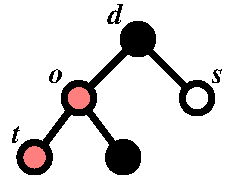
\includegraphics{pics/rbt-i}
\caption{Obecná situace při INSERTu}
\label{rbt-i}
\end{figure}

Nejprve záleží na tom, jakou barvu má $s$, strýc $t$:
\begin{enumerate}
\item $s$ je červený. Pak pouze přebarvíme $o$, $d$ a $s$ podle
obrázku \ref{rbt-i1}.
Podmínky 1 a 3 jsou splněny. Nyní $d$ může být porucha, ovšem posunutá o 2
hladiny výše. Vznikl 2tččs $(T,d)$.

\begin{figure}[!htb]
\centering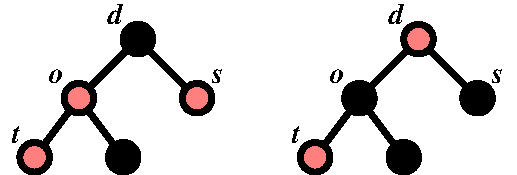
\includegraphics{pics/rbt-i1}
\caption{Oprava INSERTu přebarvením}
\label{rbt-i1}
\end{figure}

\item $s$ je černý. Záleží na tom, zda hodnota $t$ leží mezi hodnotami
$o$ a $d$ nebo ne. Jinými slovy, zda cesta $t$-$o$-$d$ obsahuje
\emph{zatáčku}.
\begin{enumerate}
\item Bez zatáčky:
Provedeme rotaci a přebarvíme podle obrázku \ref{rbt-i2a}.
Splněny budou podmínky 1, 2 i 3, tedy máme červenočerný strom.

\begin{figure}[!htb]
\centering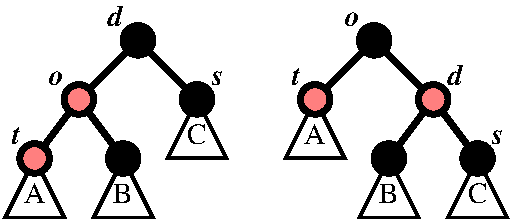
\includegraphics{pics/rbt-i2a}
\caption{Oprava INSERTu rotací a přebarvením}
\label{rbt-i2a}
\end{figure}

\item Se zatáčkou:
Provedeme dvojitou rotaci a přebarvíme podle obrázku \ref{rbt-i2b}.
Splněny budou podmínky 1, 2 i 3, opět máme rovnou červenočerný strom.

\begin{figure}[!htb]
\centering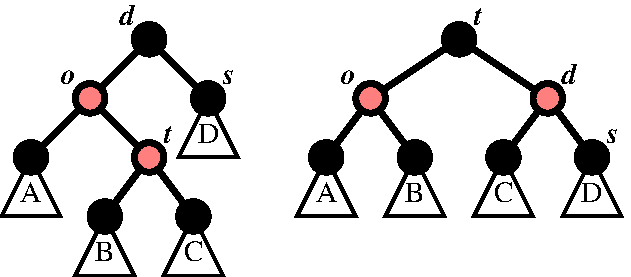
\includegraphics{pics/rbt-i2b}
\caption{Oprava INSERTu dvojitou rotací a přebarvením}
\label{rbt-i2b}
\end{figure}

\end{enumerate}
\end{enumerate}

\subsection{Operace DELETE}
Zatímco INSERT se příliš nelišil od své obdoby u AVL stromů, operace
DELETE u červenočerných stromů je oproti AVL stromům složitější
mentálně, ovšem jednodušší časově.

Situace: odstraňujeme vrchol $t$ (který nemusí reprezentovat
odstraňovaný prvek --- viz DELETE v obecných binárních vyhledávacích
stromech) a jeho syna, který je list.

Druhého syna $t$, $u$, dáme na místo smazaného $t$ a začerníme ho. Tím
máme splněné podmínky 1 a 2. Pokud byl ale $t$ černý, chybí nám na
cestách procházejících nyní vrcholem $u$ jeden černý vrchol.
\begin{defn}
Strom a jeho vrchol $(T,u)$ nazveme \emph{3-téměř červenočerný strom
(3tččs),} jestliže platí
\begin{itemize}
\item{1} Listy jsou černé. {\it (nezměněno)}
\item{2} Pokud má červený vrchol otce, je otec černý. {\it (nezměněno)}
\item{3'}
Všechny cesty z kořene do listu neprocházející $u$ mají stejný počet
černých vrcholů, nechť je to $k$. 
Všechny cesty z kořene do listu   procházející $u$ mají stejný počet
černých vrcholů, nechť je to $\ell$. 
A platí $k-1 \leq \ell \leq k$.
\end{itemize}
Když $u$ není kořen a $\ell < k$, pak řekneme, že $u$ je \emph{porucha}.
\end{defn}

\begin{pozn}
Takovému vrcholu v 3tččs se někdy říká \emph{3-porucha}.
\end{pozn}

Nechť vrchol $u$  je porucha. Pak můžeme předpokládat, že je 
obarven černě, jinak bychom ho přebarvili na černo a tím by se porucha 
odstranila a vznikl červenočerný strom.

Situace: máme 3tččs $(T,u)$, $u$ je porucha s otcem $o$, bratrem $b$ a
synovci $s1$, $s2$, viz obrázek \ref{rbt-d}.

\begin{figure}[!htb]
\centering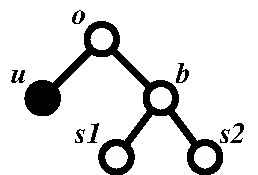
\includegraphics{pics/rbt-d}
\caption{Obecná situace při DELETE}
\label{rbt-d}
\end{figure}

\begin{samepage}
Oprava záleží na barvě vrcholu $b$:
\begin{enumerate}
\item Bratr je černý. 
Rozlišujeme dále 4 případy, z nichž jeden propaguje poruchu o hladinu
výš a ostatní skončí s červenočerným stromem.

\begin{enumerate}
\item Otec i synovci jsou černí.
Přebarvíme $b$ na červeno, viz obrázek \ref{rbt-d1a}. Dostáváme 3tččs $(T,o)$,
tedy porucha je o hladinu výše.

\begin{figure}[!htb]
\centering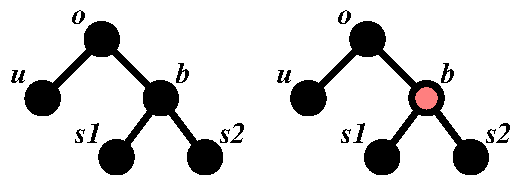
\includegraphics{pics/rbt-d1a}
\caption{Částečná oprava DELETE přebarvením}
\label{rbt-d1a}
\end{figure}
\item \label{rbt-cd1b} Otec je červený, synovci černí.
Přebarvíme otce a bratra podle obrázku \ref{rbt-d1b} a dostáváme
červenočerný strom.

\begin{figure}[!htb]
\centering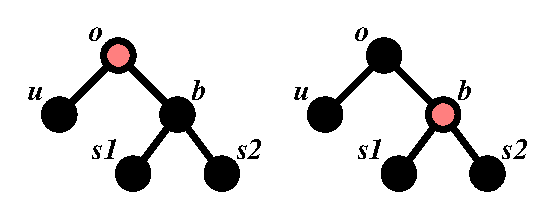
\includegraphics{pics/rbt-d1b}
\caption{Oprava DELETE přebarvením}
\label{rbt-d1b}
\end{figure}
\item \label{rbt-cd1c} Synovec $s1$, jehož hodnota leží mezi hodnotami
otce a bratra, je černý, druhý synovec je červený.
Přebarvíme a zrotujeme podle obrázku \ref{rbt-d1c}, barva otce se
nemění (tj., vrchol $b$ bude mít barvu, kterou původně měl vrchol $o$).
Dostáváme červenočerný strom.

\begin{figure}[!htb]
\centering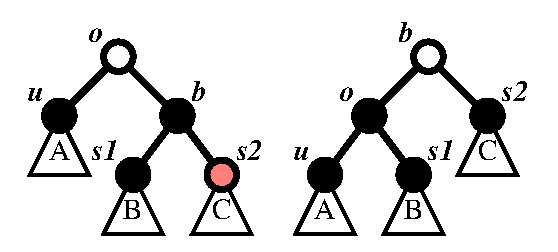
\includegraphics{pics/rbt-d1c}
\caption{Oprava DELETE přebarvením a rotací}
\label{rbt-d1c}
\end{figure}
\item \label{rbt-cd1d} Synovec $s1$, jehož hodnota leží mezi hodnotami
otce a bratra, je červený, druhý synovec má libovolnou barvu.
Přebarvíme a dvojitě zrotujeme podle obrázku \ref{rbt-d1d} (tj., vrchol $s1$ 
bude mít barvu, kterou původně měl vrchol $o$ a barva vrcholu $s2$ se nezmění).
Dostáváme červenočerný strom.

\begin{figure}[!htb]
\centering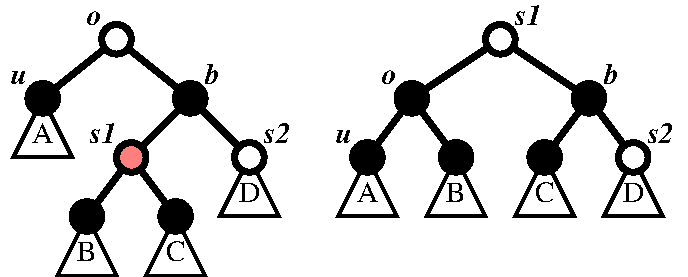
\includegraphics{pics/rbt-d1d}
\caption{Oprava DELETE přebarvením a dvojitou rotací}
\label{rbt-d1d}
\end{figure}

\end{enumerate}

\item Bratr je červený. Provedeme rotaci. 
Dostaneme strom ve tvaru, který je na \ref{rbt-d2}.
a aplikujeme předchozí případ č.1. \\
Přestože to tak na první pohled nevypadá, máme vyhráno, protože bratr 
poruchy je černý a otec červený, tedy příští oprava bude případ \ref{rbt-cd1b}, \ref{rbt-cd1c}, nebo \ref{rbt-cd1d} a skončíme s červenočerným 
stromem.

\begin{figure}[!htb]
\centering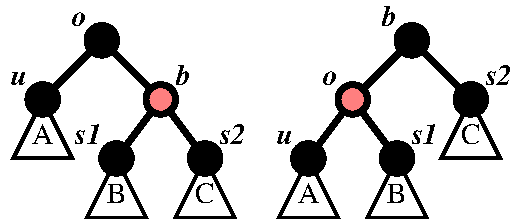
\includegraphics{pics/rbt-d2}
\caption{Částečná oprava DELETE přebarvením a rotací}
\label{rbt-d2}
\end{figure}

\end{enumerate}
\end{samepage}


\subsection{Závěry}
Pro binární vyhledávací červenočerné stromy lze implementovat MEMBER,
INSERT a DELETE tak, že vyžadují čas $O(\log n)$ a INSERT používá
nejvýše jednu (dvojitou) rotaci a DELETE používá nejvýše dvě rotace
nebo rotaci a dvojitou rotaci. 

Jsou lepší než AVL stromy, které při DELETE spotřebují až $\log n$
rotací. Oproti váhově vyváženým stromům i proti AVL stromům jsou 
červenočerné stromy jen
konstantně lepší, ale i to je dobré. Při použití binárních vyhledávacích 
stromů ve výpočetní geometrii nese informaci i rozložení prvků ve stromě, 
a tato informace se musí po provedení rotace nebo dvojité rotace aktualizovat. 
To znamená prohledání celého stromu a tedy čas $O(n)$ za každou rotaci a 
dvojitou rotaci navíc. Pro tyto problémy jsou červenočerné stromy obzvláště 
vhodné, protože minimalizují počet použitých rotací a dvojitých 
rotací\footnote{Červenočerné stromy se používají například ve 
\href{http://www.sgi.com/tech/stl/}%
standardní šablonové knihovně jazyka C++ od SGI, 
která je zahrnuta do GCC. Máte-li Linux, zkuste se podívat do
\path{/usr/include/g++-2/stl\_tree.h}; 
%pokud používáte OpenBSD, najdete
%implementaci jak červenočerných, tak splay stromů v
%\path{/usr/include/sys/tree.h}.
Co se týče "real-world" aplikací červeno-černých stromů, je možné zmínit
packet filter (PF) v OpenBSD, kde se tyto stromy používají k reprezentaci
pravidel pro firewall. Pro firewally je čas vyhodnocení jednotlivých
paketů proti pravidlům kritický. Zajímavé je, že původní implementaci PF
používala AVL stromy. Červeno-černé stromy se ukázaly jako výhodnější.
Implementaci červeno-černých stromů lze v OpenBSD najít v 
\path{/usr/include/sys/tree.h} v podobě maker jazyka C. Tento soubor 
obsahuje rovněž makra pro implementaci Splay stromů.
A pokud víte o podobně dostupných implementacích jiných
datových struktur z téhle přednášky, sem s nimi !}.

\begin{pozn}
Červenočerné stromy se používají při implementaci $(2,4)$-stromů, se
kterými se seznámíme v další kapitole. Vrchol 
se dvěma syny je nahrazen jedním černým vrcholem, vrchol se třemi syny 
je nahrazen černým vrcholem s jedním červeným synem a vrchol se čtyřmi 
syny je nahrazen černým vrcholem se dvěma syny. Pozor! Aktualizační 
operace pro $(2,4)$-stromy neodpovídají aktualizačním operacím na 
červenočerných stromech (i reprezentace prvků je odlišná).
\end{pozn}


% ==========================================================================
% Součást skript Datové struktury. ds.tex
% Authors: Martin Vidner
%	   Vladimir Kotal
\markright{$ $Id$ $}

\chapter{$(a,b)$ stromy}

% --------------------------------------------------------------------------
\section{Základní varianta}

Nechť $a, b \in \mathbb{N}, a \leq b$. Strom je $(a,b)$ strom, když
platí
\begin{enumerate}
\item Každý vnitřní vrchol kromě kořene má alespoň $a$ a nejvýše $b$
synů.
\item Kořen má nejvýše $b$ synů. Pokud $a \geq 2$, pak má alespoň 2
syny, nebo je listem.
\item Všechny cesty z kořene do listu jsou stejně dlouhé.
\end{enumerate}
\exercise
{Co by se stalo, kdybychom definici zjednodušili a místo podmínek 1 a
2 požadovali, aby \emph{každý} vrchol měl $a$ až $b$ synů?}{Nebyly by
možné malé $(a,b)$ stromy.}

\begin{figure}%[!htb]
\centering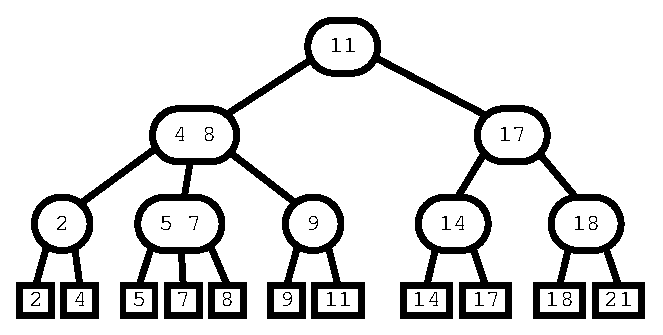
\includegraphics{pics/abt}
\caption{Příklad $(a,b)$ stromu}
\label{abt}
\end{figure}

\begin{defn}
Jsou-li synové každého vrcholu očíslováni, můžeme
definovat \emph{lexikografické uspořádání vrcholů na stejné hladině}.

$u \leq_l v$, jestliže $\text{otec } u <_l \text{otec } v$ nebo
$\text{otec } u = \text{otec } v$, $u$ je $i$-tý syn, $v$ je $j$-tý syn
a $i \leq j$.
\end{defn}

\begin{pozn}
Prvky z množiny $S$ korespondují s listy $T$ tak, že $s < s', s,s' \in S$,
právě když list odpovídající $s <_l$ list odpovídající $s'$.
\end{pozn}

Pozorování: Buď $T$ $(a,b)$ strom s hloubkou $h$. Platí
\[
2 a^{h-1} \leq \text{počet listů $T$} \leq  b^h,
\]
tedy pro libovolné $n$ má každý $(a,b)$ strom $T$ s $n$ listy 
hloubku $\Theta(\log n)$.

% ..........................................................................
\subsection{Reprezentace množiny $S$ $(a,b)$ stromem}

Mějme $S \subseteq U$, přičemž universum je lineárně uspořádané.
$(a,b)$ strom $T$ reprezentuje množinu $S$, jestliže existuje
jednoznačné přiřazení prvků $S$ listům $T$, které zachovává uspořádání.

Potřebujeme navíc podmínku
\begin{enumerate}
\item[4.] $a \geq 2$ a $b \geq 2a - 1$ 
\end{enumerate}

Struktura vnitřního vrcholu $v$:
\begin{itemize}
\item $\rho_v$ je počet synů
\item $S_v[1\ .. \ \rho_v]$ je pole ukazatelů na syny
\item $H_v[1\ .. \ \rho_v - 1]$: $H_v[i]$ je maximální prvek 
v~podstromu $S_v[i]$ 
\end{itemize}

% ..........................................................................
\subsection{MEMBER($x$) v $(a,b)$ stromu}

viz algoritmus \ref{alg:abtree.member}

\begin{algorithm}[!htb]
\caption{MEMBER pro $(a,b)$ stromy}
\label{alg:abtree.member}
\begin{algorithmic}
\STATE \COMMENT{vyhledání $x$}
\STATE $t := \text{kořen}$
\WHILE {$t$ není list}
	\STATE $i := 1$
	\WHILE {$H_t[i] < x \land i < \rho_t$}
		\STATE $i := i + 1$
	\ENDWHILE
	\STATE $t := S_t[i]$ 
\ENDWHILE
\STATE \COMMENT{testování $x$}
\IF {$t$ reprezentuje $x$}
	\STATE $x \in S$
\ELSE
	\STATE $x \notin S$
\ENDIF
\end{algorithmic}
\end{algorithm}

% ..........................................................................
\subsection{INSERT($x$) do $(a,b)$ stromu}

viz algoritmus \ref{alg:abtree.insert}

\begin{algorithm}[!htb]
\caption{INSERT pro $(a,b)$ stromy}
\label{alg:abtree.insert}
\begin{algorithmic}
\STATE vyhledání $x$
\IF {$t$ nereprezentuje $x$}
	\STATE $o := \text{otec } t$
	\STATE vrcholu $o$ přidej nového syna $t'$ 
	reprezentujícího $x$
	\STATE zařaď $t'$ na správné místo mezi jeho bratry
	a uprav $\rho_o$, $S_o$ a $H_o$
	\STATE $t := o$
	\WHILE {$\rho_t > b$}
		\STATE \COMMENT {Štěpení 
				--- můžeme provést díky podmínce 4}
		\STATE rozděl $t$ na $t_1$ a $t_2$ 
		\STATE \quad k $t_1$ dej prvních 
			$\lfloor (b+1)/2 \rfloor$ synů $t$
		\STATE \quad k $t_2$ dej zbylých 
			$\lceil (b+1)/2 \rceil$ synů $t$
		\STATE $o := \text{otec } t$
		\STATE uprav $\rho_o$, $S_o$ a $H_o$
		\STATE \COMMENT {při štěpení kořene ještě musíme
				vytvořit nový kořen}
		\STATE $t := o$
	\ENDWHILE
\ENDIF
\end{algorithmic}
\end{algorithm}

% ..........................................................................
\subsection{DELETE($x$) z $(a,b)$ stromu}

viz algoritmus \ref{alg:abtree.delete}

\begin{algorithm}[!htb]
\caption{DELETE pro $(a,b)$ stromy}
\label{alg:abtree.delete}
\begin{algorithmic}
\STATE vyhledání $x$, navíc si zapamatuj vrchol $u$, 
	v jehož poli $H_u$ je $x$
\IF {$t$ reprezentuje $x$}
	\STATE $o := \text{otec } t$
	\STATE odstraň $t$
	\STATE uprav $H_o$, $H_u$ \COMMENT {...}
	\STATE uprav $S_o$ a $\rho_o$
	\STATE $t := o$
	\WHILE {$\rho_t < a \land t \text{ není kořen}$}
		\STATE $v := \text{bezprostřední bratr } t$ 
		\IF[smíme spojit] {$\rho_v = a$}
			\STATE \COMMENT {Spojení}
			\STATE $o := \text{otec } t$
			\STATE sluč $v$ a $t$ do $t$
			\STATE uprav $\rho_o$, $S_o$ a $H_o$
			\STATE $t := o$
		\ELSE[$\rho_v > a$, spojení by mohlo mít více než $b$ synů]
			\STATE \COMMENT {Přesun}
			\STATE přesuň krajního syna $v$ do $t$
			\STATE uprav $H_{\text{otec } t}$
		\ENDIF
	\ENDWHILE
	\IF {$t$ je kořen a má jen jednoho syna}
		\STATE smaž $t$
	\ENDIF
\ENDIF
\end{algorithmic}
\end{algorithm}

% ..........................................................................
\subsection{Shrnutí}

Operace štěpení, přesun i spojení vyžadují konstantní čas. 
\begin{theorem}
Operace MEMBER, INSERT a DELETE pro $(a,b)$ stromy vyžadují čas
$O(\log n)$, kde $n$ je velikost reprezentované množiny.
\end{theorem}

S $H$ a $S$ jsme pracovali jako se seznamy, nepotřebujeme, aby to byla
pole. Tím se zjednoduší implementace. 
\mnote{Výhodnost pro vnější paměti?}

% ..........................................................................
\subsection{Jak volit parametry $(a,b)$}

Pro vnitřní paměť je vhodné $a = 2$ nebo $a=3$, $b = 2a$.
Pro vnější paměť je vhodné $a \approx 100$, $b = 2a$.

Pro minimalizaci paměťových nároků je výhodné $b = 2a-1$,
pro minimalizaci časových nároků je výhodné $b = 2a$.
\mnote{proč? prý se k tomu ještě dostaneme}

% --------------------------------------------------------------------------
\section{Další operace}

MIN, MAX (XXX)

% ..........................................................................
Pro operaci JOIN je vhodné spolu se stromem uchovávat také 
největší prvek reprezentované množiny.

\subsection{Algoritmus JOIN($T_1, T_2$) pro $(a,b)$ stromy}

Operace JOIN provede spojení dvou (a,b)-stromů $T_1$ a $T_2$ 
do jednoho (a,b)-stromu za předpokladu, že všechny prvky, které 
reprezentuje strom $T_1$ jsou menší než prvky reprezentované stromem
$T_2$.

Algoritmus najde vrchol pro stromu $T_2$, spojí stromy do jednoho (viz
obr. \ref{fig:abtree.join}) a provede štěpění.

\begin{figure}
\centering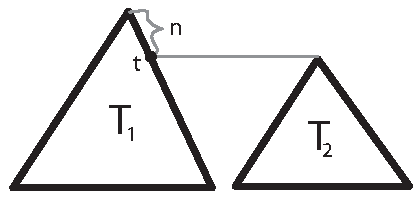
\includegraphics{pics/abtree-join}
\caption{Idea operace JOIN}
\label{fig:abtree.join}
\end{figure}

Přepis viz algoritmus \ref{alg:abtree.join}

\begin{algorithm}[!htb]
\caption{JOIN pro $(a,b)$ stromy}
\label{alg:abtree.join}
\begin{algorithmic}
\REQUIRE {$T_1$ reprezentuje $S_1$, $T_2$ reprezentuje $S_2$ 
	a $\max S_1 < \min S_2$ }
\STATE $n := \text{hloubka } T_1 - \text{hloubka } T_2$ 
\IF {$n \geq 0$}
	\STATE $t := \text{kořen } T_1$
	\WHILE {$n > 0$}
		\STATE $t := \text{poslední syn } t$
		\STATE $n := n - 1$
	\ENDWHILE
	\STATE Spoj $t$ s kořenem $T_2$ a vytvoř nový vrchol $t'$.
	\COMMENT {zde se využije znalost největšího prvku množiny $S_1$}
	\WHILE {$\rho_t > b$}
		\STATE Štěpení $t$		
		\STATE $t := \text{otec } t$
	\ENDWHILE
\ELSE
	\STATE \COMMENT {analogicky: kořen $T_2$, první syn \dots}
\ENDIF
\end{algorithmic}
\end{algorithm}

\subsubsection{Časová složitost operace JOIN}

JOIN vyžaduje čas $O(\text{rozdíl hloubek stromů}) 
\leq O(\log(|S_1| + |S_2|))$
% = O(\log(|S_1 sjednoceno S_2|)$.

% ..........................................................................
\subsection{Algoritmus SPLIT($x, T$) pro $(a,b)$ strom}

Operace SPLIT($x, T$) provede rozdělení (a,b)-stromu $T$ na dva
(a,b)-stromy $T_1$ a $T_2$ tak, že:

\begin{itemize}
  \item $T_1$ je (a,b)-strom reprezentující prvky z $S$ $< x$
  \item $T_2$ je (a,b)-strom reprezentující prvky z $S$ $> x$
\end{itemize}

kde $S$ je množina, reprezentovaná (a,b)-stromem $T$.
Na výstupu této operace dále dostaneme informaci, zda $x \in S$.

Základní myšlenkou pro implementace této operace je použití dvou zásobníků
(a,b)-stromů. Procházíme strom $T$ od kořene k listům a na každé úrovni
vložíme do prvního zásobníku ty podstromy bratrů aktuálního vrcholu, které
obsahují prvky menší než prvek reprezentovaný aktuálním vrcholem. Do
druhého zásobníku vložíme podstromy s většími prvky. 
(viz obr. \ref{fig:abtree.split})
Po projití stromu
provedeme slití těchto dvou zásobníků do stromů $T_1$ a $T_2$ pomocí
operace STACKJOIN. (viz sekce \ref{abtrees.stackjoin})

\begin{figure}
\centering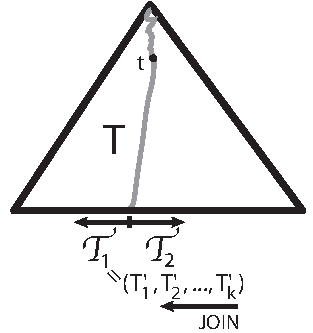
\includegraphics{pics/abtree-split}
\caption{Idea operace SPLIT}
\label{fig:abtree.split}
\end{figure}

Přepis operace SPLIT viz algoritmus \ref{alg:abtree.split}

\begin{algorithm}[!htb]
\caption{SPLIT pro $(a,b)$ stromy}
\label{alg:abtree.split}
\begin{algorithmic}
\ENSURE {Vytvoří 
	$T_1$ reprezentující $\{ s \in S: s < x \}$ a
	$T_2$ reprezentující $\{ s \in S: s > x \}$}
\STATE Nechť $Z_1$ a $Z_2$ jsou prázdné zásobníky
\STATE $t := \text{kořen } T$
\WHILE {$t$ není list}
	\STATE $i := 1$
	\WHILE {$H_t[i] < x \land i < \rho_t$}
		\STATE $i := i + 1$ 
	\ENDWHILE
	\STATE Vytvoř strom $T_1$, jehož kořen %$t_1$
	má syny $S_t[1] \dots S_t[i-1]$
	\STATE Vytvoř strom $T_2$, jehož kořen %$t_2$
	má syny $S_t[i+1] \dots S_t[\rho_t]$
	\IF {$T_1$ není jednoprvkový strom}
		\STATE Push($Z_1, T_1$)
	\ENDIF
        \IF {$T_2$ není jednoprvkový strom}
		\STATE Push($Z_2, T_2$)
	\ENDIF
	\STATE $t := S_t[i]$ 
\ENDWHILE
\IF {$t$ reprezentuje prvek různý od $x$}
	\STATE Udělej z $t$ $(a,b)$ strom a vlož ho
	do příslušného zásobníku.
\ENDIF
\STATE $T_1 := \text{STACKJOIN}(Z_1)$ \COMMENT {viz dále}
\STATE $T_2 := \text{STACKJOIN}(Z_2)$
\end{algorithmic}
\end{algorithm}

\subsubsection{Časová složitost operace SPLIT}

Čas rozřezávání stromu je úměrný jeho hloubce. Celkový čas operace
SPLIT ovšem závisí ještě na složitosti operace STACKJOIN.

% ..........................................................................
\subsection{Algoritmus STACKJOIN($Z$) pro zásobník $(a,b)$ stromů}
\label{abtrees.stackjoin}

Operace STACKJOIN provede JOIN všech (a,b)-stromů uložených na zásobníku.
Výsledkem je jediný (a,b)-strom.

Přepis viz algoritmus \ref{alg:abtree.stackjoin}

\begin{algorithm}[!htb]
\caption{STACKJOIN pro $(a,b)$ stromy}
\label{alg:abtree.stackjoin}
\begin{algorithmic}
\STATE $T := \text{Pop}(Z)$
\WHILE {$Z \ne \emptyset$}
	\STATE $T' := \text{Pop}(Z)$
	\STATE $T := \text{JOIN}(T, T')$
\ENDWHILE
\end{algorithmic}
\end{algorithm}

\subsubsection{Časová složitost operace STACKJOIN}

Nechť $Z$ obsahuje $(a,b)$ stromy $T_1 \dots T_k$, přičemž $T_1$ je
vrchol zásobníku.
Platí
\[
\forall i:\ \text{hloubka }T_i \leq \text{hloubka }T_{i+1}
\]
\begin{align*}
\text{čas STACKJOIN}
 & = \text{hloubka }T_2 - \text{hloubka }T_1 + 1 \\
 & + \text{hloubka }T_3 - \text{hloubka }T_2 + 1 \\
 & + \dots \\
 & + \text{hloubka }T_k - \text{hloubka }T_{k-1} + 1 \\
 & = \text{hloubka }T_k - \text{hloubka }T_1 + \text{počet JOINů} \\
 & = O(\text{hloubka }T) = O(\log |S|)
\end{align*}

Tedy i operace SPLIT vyžaduje čas $O(\log |S|)$.

% ..........................................................................
\subsection{Algoritmus FIND($T, k$) pro $(a,b)$ strom}

Nalezení $k$-tého nejmenšího prvku.

Rozšíříme reprezentaci stromu a každému vnitřnímu vrcholu $v$ přidáme:
\begin{itemize}
\item $K_v[1\ .. \ \rho_v]$: $K_v[i]$ je počet listů
v~podstromu $S_v[i]$ 
\end{itemize}

viz algoritmus \ref{alg:abtree.find}

\begin{algorithm}[!htb]
\caption{FIND pro $(a,b)$ stromy}
\label{alg:abtree.find}
\begin{algorithmic}
\STATE $t := \text{kořen }T$
\WHILE {$t$ není list}
	\STATE $i := 1$
	\WHILE {$K_t[i] < k \land i < \rho_t$}
		\STATE $k := k - K_t[i]$ 
		\STATE $i := i + 1$ 
	\ENDWHILE
	\STATE $t := S_t[i]$ 
\ENDWHILE
\IF {$k > 1$}
	\STATE \textbf{return} nil \COMMENT {$k > |S|$}
\ELSE
	\STATE \textbf{return} $t$
\ENDIF
\end{algorithmic}
\end{algorithm}

Časová složitost je opět logaritmická, přičemž dříve uvedené operace
nejsou zpomaleny tím, že aktualizují pole (seznam) $K$.

% ..........................................................................
\section{A-sort}

Na první pohled se zdá, že použití $(a,b)$ stromů ke třídění není
výhodné. Paměťové nároky budou oproti běžnému třídění v poli asi
pětkrát větší. Aby se tedy třídění $(a,b)$ stromem vyplatilo, muselo
by přinést zvýšení rychlosti. V této části předvedeme, že to skutečně
je možné, jestliže vstupní data jsou již částečně setříděná.

Pro účely A-sortu rozšíříme reprezentaci takto:
\begin{itemize}
\item Listy stromu jsou propojeny do seznamu
\item Je známa cesta z nejmenšího (nejlevějšího) listu do kořene
(uložená např. v zásobníku)
\end{itemize}

Použijeme $(2,3)$-strom. Proč, to si zdůvodníme až po odvození složitosti
A-sortu.

Nechť vstupní posloupnost je $a_1, \dots, a_n$. Postupně odzadu
vkládáme její prvky do stromu modifikovaným INSERTem:

\begin{algorithmic}
\STATE $k := n$
\WHILE {$k > 1$}
	\STATE A-INSERT($a_k$)
	\STATE $k := k - 1$
\ENDWHILE
\end{algorithmic}

Na konci přečteme setříděnou posloupnost pomocí spojového seznamu
listů.

\subsection{A-INSERT}

A-INSERT (viz algoritmus \ref{alg:abtree.a-insert}) pracuje
téměř stejně jako původní INSERT - najde správný list a potom
případně přidá nový prvek. K nalezení správného listu ovšem využívá
cestu z nejmenšího listu. (viz obr. \ref{fig:abtree.a-insert})

\begin{figure} 
\centering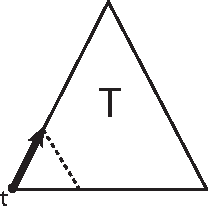
\includegraphics{pics/a-insert}
\caption{Idea algoritmu A-INSERT}
\label{fig:abtree.a-insert}
\end{figure}

Zde uvedená verze A-INSERTu odstraňuje 
duplicitní prvky, operaci lze pochopitelně upravit tak, že nechává 
duplicitní prvky, které zůstávají ve stejném pořadí.

\begin{algorithm}[!htb]
\caption{A-INSERT($x$)}
\label{alg:abtree.a-insert}
\begin{algorithmic}
\STATE \COMMENT {Nalezení}
\STATE $t := \text{nejmenší list stromu } T$
\REPEAT
	\STATE $t := \text{otec } t$
\UNTIL {$t \text{ je kořen} \lor x \leq H_t[1]$}
\STATE \COMMENT {nyní jako v původním INSERTu, pouze jsme jinak
inicializovali $t$}
\WHILE {$t$ není list}
	\STATE $i := 1$
	\WHILE {$H_t[i] < x \land i < \rho_t$}
		\STATE $i := i + 1$
	\ENDWHILE
	\STATE $t := S_t[i]$ 
\ENDWHILE
\STATE \COMMENT {Přidání}
\IF {$t$ nereprezentuje $x$}
	\STATE $o := \text{otec } t$
	\STATE vrcholu $o$ přidej nového syna $t'$ 
	reprezentujícího $x$
	\STATE zařaď $t'$ na správné místo mezi jeho bratry
	a uprav $\rho_o$, $S_o$ a $H_o$
	\STATE $t := o$
	\WHILE {$\rho_t > b$}
		\STATE \COMMENT {Štěpení 
				--- můžeme provést díky podmínce 4}
		\STATE rozděl $t$ na $t_1$ a $t_2$ 
		\STATE \quad k $t_1$ dej prvních 
			$\lfloor (b+1)/2 \rfloor$ synů $t$
		\STATE \quad k $t_2$ dej zbylých 
			$\lceil (b+1)/2 \rceil$ synů $t$
		\STATE $o := \text{otec } t$
		\STATE uprav $\rho_o$, $S_o$ a $H_o$
		\STATE \COMMENT {při štěpení kořene ještě musíme
				vytvořit nový kořen}
	\ENDWHILE
\ENDIF
\end{algorithmic}
\end{algorithm}

\subsection{Složitost A-sortu}

Čas A-sortu
= $\sum$ času vyhledání + $\sum$ času přidání + čas vytvoření výstupní
posloupnosti.
Čas vytvoření výstupní posloupnosti = $O(n)$.

$\sum \text{času přidání} 
= \text{počet přidaných vrcholů} \cdot \text{čas přidání vrcholu}
+ \text{počet štěpení} \cdot \text{čas štěpení}
= O(n) \cdot O(1)
+ \text{počet štěpení} \cdot O(1).$ 
Protože se zde neprovádí operace DELETE, lze každému štěpení přiřadit 
vnitřní vrchol, který byl při tomto štěpení vytvořen (štěpení rozdělí 
vrchol $t$ na dva vrcholy $t_1$ a $t_2$, budeme předpokládat, že 
vrchol $t_1$ je pokračováním vrcholu $t$ a vrchol $t_2$ je vrchol 
vzniklý při štěpení). Tedy počet štěpení je menší než počet vnitřních 
vrcholů (při štěpení kořene vzniká navíc ještě nový kořen),  
tedy $\sum \text{času přidání} = O(n).$

Čas A-sortu tedy závisí hlavně na celkovém čase vyhledání prvků.
Označme
\[
f_i = |\{ j > i:\ a_j < a_i \}|,
\]
tedy počet prvků posloupnosti, které v nesetříděné posloupnosti
následují $a_i$, ale v setříděné patří před $a_i$. Při vyhledání $a_i$
ve stromu vyjadřuje $f_i$ počet listů nalevo od $a_i$. Čas
vyhledání $a_i$ je tedy $O(\log f_i)$ a celkový čas vyhledání je 
$O(\sum \log f_i)$.
\mnote{ošetřit $\log 0$}

Hodnota $F = \sum f_i$, zvaná 
\emph{počet inverzí}, \mnote{nebo transpozic? standardní termín?}%
vyjadřuje uspořádanost vstupní
posloupnosti. Pro správně uspořádanou posloupnost je $F = 0$, pro
obráceně uspořádanou posloupnost je $F = n (n-1) / 2$. To jsou také
mezní hodnoty, jichž může $F$ nabývat.

Z vlastností logaritmu a srovnáním geometrického a aritmetického
průměru dostáváme
\[
\sum \log f_i = \log \prod f_i = n \log \sqrt[n]{\prod f_i}
\leq n \log (F/n).
\]

A-sort tedy vyžaduje čas $O(n \max(1, \log((F+1)/n)))$. V nejhorším
případě to je $O(n \log n)$ a Mehlhorn a Tsakalidis ukázali, že A-sort
je lepší než Quicksort v případě, že $F \leq 0.02 n^{1.57}$.
Naproti tomu Insertsort, jednoduchý algoritmus, který postupně
lineárním prohledáním zatřiďuje prvky pole do jeho již setříděného
počátečního úseku, vyžaduje čas $O(n + F)$, což je v nejhorším případě
$O(n^2)$.

Zbývá ještě zdůvodnit, proč použít $(2,3)$-stromy. Víme, že $(2,3)$-stromy 
mají nejmenší prostorové nároky mezi $(a,b)$-stromy. Na druhé straně však 
$(2,3)$-stromy v obecném přépadě vyžadují zbytečně mnoho vyvažovacích 
operací, a proto jsou výrazně pomalejší než např. $(2,4)$-stromy. Protože 
však A-sort nepoužívá operaci DELETE, ukázali jsme (viz počet operací 
Štěpení), že pro A-sort to není pravda. Zde $(2,3)$-stromy patří mezi 
nejrychleji pracující $(a,b)$-stromy.

% --------------------------------------------------------------------------
\section{Paralelní přístup do $(a,b)$ stromů}

Při operacích INSERT a DELETE jsme nejprve sestupovali stromem dolů až
k listům, potom jsme se vraceli nahoru a štěpili nebo spojovali
vrcholy. To znemožňuje dovolit paralelní přístup do stromu. Procesu,
který je ve fázi vyhledání, by se mohlo stát, že mu jiný proces změní
strom ``pod rukama''. Stávající operace INSERT a DELETE tedy požadují
výlučný přístup ke stromu.
\par
Nyní předvedeme paralelní verzi těchto operací, kde se štěpení nebo
spojování provádí již při sestupu. Potom již není nutné se vracet a je
tedy možné rovnou odemykat části stromu, ke kterým již daný proces
nebude přistupovat. Cenou za tento přístup jsou zbytečná
štěpení/spojení.
\mnote{udělat obrázek ilustrující zbytečná š/s}

Potřebujeme omezit $b$: podmínku $b \geq 2a - 1$ zpřísníme na
\begin{enumerate}
\item[4'.] $a \geq 2$ a $b \geq 2a$ 
\end{enumerate}

% ..........................................................................
\subsection{Paralelní INSERT($x$) do $(a,b)$ stromu}

viz algoritmus \ref{alg:abtree.par.insert}

\begin{algorithm}[!htb]
\caption{paralelní INSERT pro $(a,b)$ stromy}
\label{alg:abtree.par.insert}
\begin{algorithmic}
\STATE $o := \text{lock}(\text{nadkořen})$ \COMMENT {Nadkořen
je implementační pomůcka. Slouží k zamknutí
přístupu k celému stromu a uchovává $\max(S)$}
\STATE $t := \text{kořen}$ 
\STATE \COMMENT {Invariant mezi průchody cyklem:
	$o$ je otec $t$, $o$ je jediný vrchol zamknutý tímto procesem.}
\WHILE {$t$ není list}
	\STATE $i := 1$
	\WHILE {$i < \rho_t \land H_t[i] < x$}
		\STATE $i := i + 1$
	\ENDWHILE
	\STATE $s := S_t[i]$ 
	\STATE \COMMENT {preventivní rozštěpení:}
	\IF {$\rho(t) = b$}
		\STATE rozděl $t$ na $t_1$ a $t_2$: \COMMENT {viz 4'}
		\STATE \quad k $t_1$ dej prvních 
			$\lfloor (b+1)/2 \rfloor$ synů $t$
		\STATE \quad k $t_2$ dej zbylých 
			$\lceil (b+1)/2 \rceil$ synů $t$
		\STATE \quad $t_1$ předchází $t_2$
		\STATE uprav $\rho_o$, $S_o$ a $H_o$
		\STATE \COMMENT {implic.: uprav $\rho_{t_1}$, \dots, $H_{t_2}$}
		\STATE \COMMENT {při štěpení kořene ještě musíme
				vytvořit nový kořen}
		\STATE $n := t_j$, kde $s$ je syn $t_j$
	\ELSE
		\STATE $n := t$
	\ENDIF
	\STATE lock($n$) 
	\STATE unlock($o$) 
	\STATE $o := n$
	\STATE $t := s$
\ENDWHILE
\IF {$t$ nereprezentuje $x$}
	\STATE vrcholu $o$ přidej nového syna $t'$ 
	reprezentujícího $x$
	\STATE zařaď $t'$ na správné místo mezi jeho bratry
	a uprav $\rho_o$, $S_o$ a $H_o$
\ENDIF
\STATE unlock($o$)
\end{algorithmic}
\end{algorithm}

% ..........................................................................
\subsection{Paralelní DELETE($x$) z $(a,b)$ stromu}

viz algoritmus \ref{alg:abtree.par.delete}

\begin{algorithm}[!htb]
\caption{paralelní DELETE pro $(a,b)$ stromy}
\label{alg:abtree.par.delete}
\begin{algorithmic}
\STATE $o := \text{lock}(\text{nadkořen})$ \COMMENT {Nadkořen
je implementační pomůcka. Slouží k zamknutí
přístupu k celému stromu a uchovává $\max(S)$}
\STATE $t := \text{kořen}$ 
\STATE $h := \textbf{nil}$ \COMMENT 
	{Jakmile $h \neq \textbf{nil}$, 
	$x \in H_h$ a $h$ bude zamčený do konce procesu.}
\STATE \COMMENT {Invariant mezi průchody cyklem:
	$o$ je otec $t$, $o$ je kromě $h$ jediný vrchol
	zamknutý tímto procesem.}
\WHILE {$t$ není list}
	\STATE $i := 1$
	\WHILE {$i < \rho_t \land H_t[i] < x$}
		\STATE $i := i + 1$
	\ENDWHILE
	\IF {$H_t[i] = x$}
		\STATE $h := t$
	\ENDIF
	\STATE $s := S_t[i]$ 
	\STATE \COMMENT {preventivní spojení/přesun:}
	\IF {$\rho(t) = a$}
		\STATE $v := \text{bezprostřední bratr } t$ %bratr[fi]=_v_eli
		\IF[smíme spojit] {$\rho_v = a$}
			\STATE \COMMENT {Spojení}
			\STATE sluč $v$ a $t$ do $t$ \COMMENT {viz 4'}
			\STATE uprav $\rho_o$, $S_o$ a $H_o$
			\STATE $t := o$
		\ELSE[$\rho_v > a$, spojení by mělo více než $b$ synů]
			\STATE \COMMENT {Přesun}
			\STATE přesuň krajního syna $v$ do $t$
			\STATE uprav $H_o$, $H_v$ a $H_t$
		\ENDIF
	\ENDIF
	\STATE lock($t$) 
	\IF {$o \neq h$}
		\STATE unlock($o$)
	\ENDIF
	\STATE $o := t$
	\STATE $t := s$
\ENDWHILE
\IF {$t$ reprezentuje $x$}
	\STATE odstraň $t$
	\STATE uprav $H_o$, $H_h$
	\STATE uprav $S_o$ a $\rho_o$
	\STATE unlock($h$)
\ENDIF
\STATE unlock($o$)
\end{algorithmic}
\end{algorithm}


% --------------------------------------------------------------------------
\section{Složitost posloupnosti operací na $(a,b)$ stromu}

A-sort funguje jednak proto, že v předtříděné posloupnosti rychle
najde místo, kam se má vkládat, jednak proto, že se při samých
INSERTech ({\it a díky správným $a$, $b$?}) provádí málo
vyvažovacích kroků. V této sekci se podíváme na počet vyvažovacích
kroků pro posloupnost operací INSERT a DELETE.

Nechť $b \geq 2a$.
\begin{theorem}
Mějme posloupnost $n$ operací INSERT a DELETE aplikovanou na prázdný
$(a,b)$ strom. Označme $P$ počet přesunů při provádění posloupnosti,
$SP$ počet spojení a $ST$ počet štěpení. Dále označme $P_h$, $SP_h$ a
$ST_h$ počet přesunů. spojení a štěpení, které nastanou ve výšce $h$
(listy mají výšku 0).

Nechť
\begin{equation}
\begin{split}
% this is ``occult alignment'' :)
c = \min
 &\left(
   \phantom{b - \vphantom{x}}
        \min \left( 2a-1, \left\lceil \frac{b+1}{2}\right\rceil  \right) - a, 
  \right.\\
 &\left.
		\phantom{\left(
		\vphantom{\left. \frac xy\right.}
		\right.}
    b - \max \left( 2a-1, \left\lfloor\frac{b+1}{2}\right\rfloor \right)
   \phantom{\vphantom{x} - a}
  \right)
\end{split}
\end{equation}

Pak platí
%\renewcommand{\labelenumi}{\alph{enumi}}
\begin{eqnarray}
P &\leq& n \\
\label{ab-v-stsp}
(2c-1)ST + cSP &\leq& n + c + \frac c{a+c-1} (n-2) \\
\label{ab-v-sthsph}
P_h + SP_h + ST_h &\leq& \frac{2 n^{c+2}}{(c+1)^h} 
\end{eqnarray}
\end{theorem}

Platí $c \geq 1$ (při $b = 2a$ dokonce $c = 1$). Z toho
\begin{equation}
ST + SP \leq \frac nc + 1 + \frac{n-2}a,
\end{equation}
tedy lineárně vzhledem k $n$.

Pro paralelní verze INSERT a DELETE platí obdobná věta, když 
$b \geq 2a + 2$.

Pro důkaz použijeme \emph{bankovní paradigma}: datovou strukturu
ohodnotíme podle toho, jak je ``uklizená''. Operace, které datovou
strukturu ``uklidí'', zvětší její ``zůstatek na účtě''. Ty, které ji
``naruší'', zůstatek zmenší. Potom najdeme vztah mezi zůstatkem a
spotřebovaným časem.
{\it Tohle pokulhává. Myslel jsem si, že zůstatek je něco jako čas v
konzervě, který si pomalé operace berou od rychlých \dots, ale  v
tomhle případě to asi funguje jinak.}
\mnote{vyjasnit}
\mnote{použiju $z$ jako zůstatek místo $b$ jako balance, protože
souvislost s vyvažováním stromu je zde spíš matoucí}

$(a,b)$ stromy jsou uklizené, když mají vrcholy počet synů někde
uprostřed mezi $a$ a $b$. Tehdy nenastane v brzké době vyvažovací
operace. V tomto smyslu definujme:
\begin{align}
z(v) &=
	\min ( \rho_v - a, b - \rho_v, c ) 
	&&\text{$v$ je vnitřní vrchol různý od kořene}\\
z(\text{kořen}) &=
        \min ( \rho_v - 2, b - \rho_v, c ) 
\end{align}

Pro strom $T$ definujme 
\[
z(T) = \sum_{v \in T} z(v)
\]
\[
z_h(T) = \sum_{\substack{v \in T\\v \text{ má výšku } h}} z(v)
\]
Platí
\[
z(T) = \sum_h z_h(t)
\]

Podobně jako u červenočerných stromů definujme parciální $(a,b)$-strom:
\begin{defn}
$(T,v)$ je \emph{parciální $(a,b)$-strom,} když $v$ je vnitřní vrchol $T$
různý od kořene a
kromě $v$ jsou splněny podmínky pro $(a,b)$-strom a
$a-1 \leq \rho_v \leq b+1$.
\end{defn}

Z definice zůstatku vyplývají tyto vlastnosti:
\begin{align}
\label{ab-1}
  \rho_v = a-1 \text{ nebo }b+1 &\implies z(v) = -1\\
\label{ab-0}
  \rho_v = a \text{ nebo } b    &\implies z(v) = 0\\
\label{ab-spojeni}
  \rho_v = 2a-1                 &\implies z(v) = c\\
\label{ab-stepeni}
  \rho_u = \left\lfloor\frac{b+1}{2}\right\rfloor \land
  \rho_v = \left\lceil \frac{b+1}{2}\right\rceil
                                &\implies z(u)+z(v) \geq 2c - 1\\
\label{ab-presun}
  |\rho_u - \rho_v| \leq 1      &\implies z(u) \geq z(v) - 1
\end{align}

\subsection{Přidání/ubrání listu}

Mějme $(a,b)$-strom $T$ a přidáme nebo ubereme list, jehož otec je $v$.
Pak vznikne parciální $(a,b)$-strom $(T',v)$ a platí:
\begin{align}
  z_1(T')        & \geq z_1(T) - 1\\
  z_h(T')        & = z_h(T) \quad h>1\\
  z(T')          & \geq z(T) - 1
\end{align}

\subsection{Štěpení}

Mějme parciální $(a,b)$-strom $(T,v)$, kde $v$ je ve výšce $h$.
Nechť $T'$ vznikl \emph{štěpením $v$}. 
Pak $(T',\text{otec }v$ je parciální $(a,b)$-strom a platí:
\begin{align}
  z_h(T')       & \geq 2c + z_h(T)
	\qquad\text{z \ref{ab-1} a \ref{ab-stepeni}}\\
  z_{h+1}(T')   & \geq z_{h+1}(T) - 1\\
  z_i(T')       & = z_i(T) \quad i \neq h, h+1\\
  z(T')         & \geq z(T) + 2c - 1
\end{align}

\subsection{Spojení}

Mějme parciální $(a,b)$-strom $(T,v)$, kde $\rho_v = a-1$ a 
$v$ je ve výšce $h$, $y$ je bezprostřední bratr $v$.
Nechť $\rho_y = a$ a $T'$ vznikl \emph{spojením $v$ a $y$}. 
Pak $(T',\text{otec }v$ je parciální $(a,b)$-strom a platí:
\begin{align}
  z_h(T')       & \geq c + 1 + z_h(T)
	\qquad\text{z \ref{ab-1}, \ref{ab-0} a \ref{ab-spojeni}}\\
  z_{h+1}(T')   & \geq z_{h+1}(T) - 1\\
  z_i(T')       & = z_i(T) \quad i \neq h, h+1\\
  z(T')         & \geq z(T) + c
\end{align}

\subsection{Přesun}

Mějme parciální $(a,b)$-strom $(T,v)$, kde $\rho_v = a-1$ a 
$v$ je ve výšce $h$, $y$ je bezprostřední bratr $v$.
Nechť $\rho_y > a$ a $T'$ vznikl \emph{přesunem syna od $y$ k $v$}. 
Pak $T'$ je $(a,b)$-strom a platí:
\begin{align}
  z_h(T')       & \geq z_h(T)
	\qquad\text{z \ref{ab-1}, \ref{ab-0} a \ref{ab-presun}}\\
  z_i(T')       & = z_i(T) \quad i \neq h\\
  z(T')         & \geq z(T)
\end{align}

Nechť po skončení posloupnosti operací máme $(a,b)$-strom $T_k$.
Sečteme předchozí výsledky:
\begin{equation}
\label{eq:ab-secti}
  z(T_k) \geq (2c - 1)ST + c SP - n  
\end{equation}

\begin{align}
  z_1(T_k)      & \geq 2c ST_1 + (c+1) SP_1 - n\\
  z_h(T_k)      & \geq 2c ST_h + (c+1) SP_h - ST_{h-1} - SP_{h-1} \quad h>1
\end{align}
Vadí nám, že jsou ve výrazu i spojení a štěpení z jiné hladiny.

$c \geq 1 \implies 2c \geq c+1$.
\[
  z_h(T_k) \geq (c+1) (ST_h + SP_h) - ST_{h-1} - SP_{h-1}
\]
\begin{align}
  ST_h + SP_h 
&  \leq \frac{z_h(T_k)}{c+1} + \frac{ST_{h-1} + SP_{h-1}}{c+1}
  \leq \frac{z_h(T_k)}{c+1} + 
         \frac{z_{h-1}(T_k)}{(c+1)^2} + 
         \frac{ST_{h-2} + SP_{h-2}}{(c+1)^2}\\
&  \leq \left( \sum_{i=0}^{h-1} \frac{z_{h-i}(T_k)}{(c+1)^{i+1}} \right) + 
         \frac{ST_0 + SP_0}{(c+1)^h}
                \qquad\text{$j=h-i$, rozšíříme $(c+1)^{h-i}$}\\
\label{ab-sthsph}
&  = \left( \sum_{j=1}^h \frac{z_j(T_k)(c+1)^j}{(c+1)^{h+1}} \right) + 
         \frac{n}{(c+1)^h}
\end{align}

Nechť $T$ je $(a,b)$-strom s $m$ listy. Chceme shora odhadnout $z(T)$.
\begin{equation}
  m_j = \text{počet vnitřních vrcholů různých od kořene}
  \begin{cases}
    \text{s právě $a+j$ syny}   & \text{když}\ j \in\intrange{0}{c-1}\\
    \text{s alespoň $a+j$ syny} & \text{když}\ j = c
  \end{cases}
\end{equation}

Když $v$ je vnitřní vrchol různý od kořene s právě $a+j$ syny,
$j \in\intrange{0}{c-1}$,
pak $z(v) \leq j$.

Když $v$ je vnitřní vrchol různý od kořene s alespoň $a+c$ syny,
pak $z(v) \leq c$.

Tedy
\begin{equation}
  \label{eq:ab-mj}
  z(T) \leq c + \sum_{j=0}^c j m_j = *
\end{equation}

Spočítáme hrany v $T$: nalevo jsou hrany vycházející z kořene a
vnitřních vrcholů, napravo jsou hrany přicházející do vnitřních
vrcholů a listů.
\begin{equation}
2 + \sum_{j=0}^c (a+j) m_j \leq
\text{počet hran}
= \left( \sum_{j=0}^c m_j \right) + m
\end{equation}
Tedy $m-2 \geq \sum_{j=0}^c (a+j-1) m_j$.

\begin{equation}
  *
  =    c + \sum_{j=0}^c \frac{j}{a+j-1}(a+j-1) m_j 
  \leq c + \sum_{j=0}^c \frac{c}{a+c-1}(a+j-1) m_j 
  \leq c + \frac{c}{a+c-1} (m-2)
\end{equation}

Spojením tohoto výsledku s \ref{eq:ab-secti} dostaneme \ref{ab-v-stsp}.

K důkazu \ref{ab-v-sthsph} využijeme \ref{ab-sthsph}.
\begin{equation}
  m_{h,j} = \text{počet vnitřních vrcholů ve výšce $h$}
  \begin{cases}
    \text{s právě $a+j$ syny}   & \text{když}\ j \in\intrange{0}{c-1}\\
    \text{s alespoň $a+j$ syny} & \text{když}\ j = c
  \end{cases}
\end{equation}

\begin{equation}
  z_h(T) \leq \sum_{j=0}^c j m_{h,j}
\end{equation}
\begin{equation}
  \sum_{j=0}^c m_{h,j}
   = \text{počet vrcholů ve výšce $h$} 
  \geq \sum_{j=0}^c (a+j) m_{h+1,j}
\end{equation}
\begin{equation}
\label{ab-x}
  \sum_{j=0}^c j m_{h,j}
  \leq \sum_{j=0}^c m_{i-1,j} - a \sum_{j=0}^c m_{i,j} 
\end{equation}
\begin{align}
   \sum_{i=1}^h z_i(T_k)(c+1)^i
 & \leq \sum_{i=1}^h (c+1)^i \left( \sum_{j=0}^c j m_{i,j} \right) \\
\intertext{označme $s_i = \sum_{j=0}^c m_{i,j}$}
 & \stackrel{\text{\ref{ab-x}}}{\leq} 
        \sum_{i=1}^h (c+1)^i \left( s_{i-1} - a s_i \right) \\
 & = (c+1)s_0 - (c+1)^h a s_h + 
        \sum_{i=2}^h (c+1)^i \left( s_{i-1} - \frac{a}{c+1} s_{i-1} \right) \\
 & \leq (c+1) m \qquad\text{protože $\frac{a}{c+1} \geq 1$ a $s_0 = m$}
\end{align}

\[
ST_h + SP+h \leq \frac{m}{(c+1)^h} + \frac{n}{(c+1)^h} \leq \frac{2n}{(c+1)^h}
\]
\[
P_h \leq SP_{h-1} - SP_h \leq SP_{h-1} + ST_{h-1} \leq \frac{2n}{(c+1)^{h-1}}
\]
Tím dostáváme \ref{ab-v-sthsph}:
\[
ST_h + SP_h + P_h \leq \frac{2 n (c+2)}{(c+1)^h}
\]


% --------------------------------------------------------------------------
\section{Propojené $(a,b)$ stromy s prstem}

Variantou $(a,b)$ stromů jsou $(a,b)$ stromy, které mají propojené
jednotlivé hladiny a dále obsahují ukazatel na jeden z listů.
Těmto stromům se také někdy říká jenom stromy s prstem (předpokládá se, že
jsou propojené) nebo hladinově propojené. V anglické literatuře se
vyskytují pod pojmem \emph{finger trees}.
\par
Struktura vnitřního vrcholu $v$ obsahuje následující položky: 
\begin{itemize}
\item $\rho(v) =$ počet synů $v$ 
\item $Syn[1..\rho(v)]$ je pole ukazatelů na syny vrcholu $v$
\item $Hod[1..\rho(v)]$ je pole hodnot, platí 
\item $Hod(i-1) <$ prvky reprezentované v podstromu $i$-tého syna $\leq Hod(i)$ 
\item $otec(v)$ = ukazatel na otce vrcholu $v$
\end{itemize}

\begin{tabular}{l}
Předchůdce$(v)$ \\
Následník$(v)$
\end{tabular}
$\Bigl\}$
\begin{tabular}{l}
ukazatele na bezprostř. předchůdce (následníka) v na hladině vrcholu $v$ \\
(v lexikogr. uspořádání)
\end{tabular}
\par

$h$ - hodnota, která leží mezi největším prvkem podstromu v a nejmenším
prvek podstromu následníka.

Příklad (a,b)-stromu s prstem je vidět na obr. \ref{fig.abtree.finger}

\begin{figure}[!htb]
\centering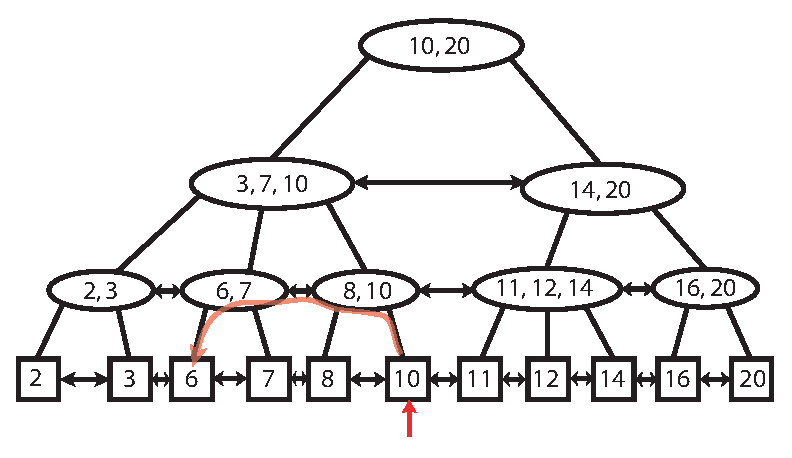
\includegraphics{pics/abtree-finger}
\caption{(a,b)-strom s prstem při provedení operace MEMBER(6)} 
\label{fig.abtree.finger}
\end{figure} 

\subsection{Algoritmus MEMBER}

Viz algoritmus \ref{alg:abtreesfing.member}

\mnote{XXX alg. MEMBER je velmi podivny, prepracovat}

\begin{algorithm}[!htb]
\caption{MEMBER (a,b) stromy s prstem}
\label{alg:abtreesfing.member}
\begin{algorithmic}
\STATE MEMBER(x)
\STATE 1) Nechť $y$ je hodnota, na kterou ukazuje Prst.
  \IF {$x < y$} 
    \STATE pokračuju 2)
  \ELSE
    \STATE 3)
  \ENDIF
\STATE 2) $v \leftarrow otec(y)$
  \STATE dokud $x < h$(Předchůdce(Předchůdce($v$))
   \STATE jdu na otce(Předchůdce($v$))
  \STATE v opačném případě
    \STATE když $x \leq$ h(Předchůdce($v$)) pak
    \STATE $v$ $\leftarrow$ Předchůdce($v$)
    \STATE a pokračuji normálním vyhledáváním
\STATE 3) symetrické ke 2)
\end{algorithmic}
\end{algorithm}

\subsection{Algoritmus FINGER}

FINGER($x$) \\
nastaví hodnotu na list, který reprezentuje prvek nejbližší k x.

Použití: \\
když lze operace přirozeným způsobem rozdělit do segmentů a operace v ?
segmentu mají operace blízko sebe
\par

\begin{itemize}
\item vyhledání $x$ vyžaduje čas $O(1 + \log(l))$
\item nastavím prst na nějakou vhodnou hodnotu
\end{itemize}

\begin{theorem}
Nechť $T$ je propojovaný (a,b) strom s prstem a nechť $P$ je posloupnost
příkazů MEMBER, INSERT, DELETE, FINGER, kterou provedeme na $T$.
Pak $P$ vyžaduje čas $O(log(n) + \text{čas na vyhledání})$
kde $n$ je velikost množiny reprezentované stromem $T$. ($b \geq 2a$)
\end{theorem}

\subsection{Amortizovaná složitost}

Vezmeme posloupnost $n$ operací, spočítáme maximální čas, který vyžadují a
ten vydělíme $n$. 
Limita takto získaných čísel pro $n \rightarrow \infty$ je amortizovaná
složitost.

\subsubsection{Bankovní paradigma}

Použijeme následující značení pro přechodu mezi stavy (situacemi):
$D \stackrel{o}{\rightarrow} D'$

\begin{itemize}
\item $D$ - vstupní situace 
\item $o$ - operace 
\item $D'$ - výstupní operace 
\end{itemize}

Amortizovaná složitost operace $o$ je Čas$(O) + bal(D') - bal(D)$,
kde $bal()$ je ohodnocení konfigurace.

$D_0 \stackrel{O_1}{\rightarrow} D_1 \stackrel{O_2}{\rightarrow} D_2 \rightarrow \ldots \rightarrow D_n$

$$\sum_{i=1}^{n} \text{čas}(O_i) + bal(D_n) - bal(D_0) = \sum a(O_i) \leq
\sum i(O_i)$$

Obvykle platí, že $bal \geq 0$ nebo $bal \leq 0$. \\
Když $bal \geq 0$, pak: \\
  $$\sum \text{čas}(O_i) \leq \sum a(O_i) + bal(D_0) \leq \sum i(O_i) + bal(D_0)$$
Když $bal \leq 0$, pak \\
  $$\sum \text{čas}(O_i) \leq \sum a(O_i) - bal(D_n) \leq \sum i(O_i) - bal(D_0)$$

Začínáme na prázdném (a,b) stromě $\rightarrow bal = 0$.

XXX nechybi tady neco ?



% ==========================================================================
% Součást skript na Datové struktury. Viz main.tex
% přepsal Vladimír Kotal, 2003


% nasleduje prednaska z 19.3.2003, přepsal Vladimír Kotal

\markright{$ $Id$ $}

\chapter{Samoopravující se struktury}

Upravující algoritmy pracují na seznamech, mohou přemístit prvek, 
který je argumentem operace. (pokud zůstává v seznamu) 
Čas na vyhledání - to je pozice hledaného prvku. Pokud není v seznamu, je
to délka seznamu + 1.
\par

Pokud byl prvek na $i$-tém místě a přesune se na $j$-té, tak je-li\\
  $j < i$, provedou $i-j$ volných výměn\\
  $j > i$, provedou $j-i$ placených výměn
\par

Volné výměny se nezapočítávají do složitosti.
Pokud x není v seznamu při operaci INSERT(x), tak předpokládejme, že je na
1. pozici po ukončení seznamu.


% --------------------------------------------------------------------------
\section{Seznamy}

{\mnote XXX operace nad obycejne seznamy jsou velmi jednoduche. Všechny
musí lineárně projít celý seznam než provedou danou operaci.}

MEMBER
INSERT
DELETE


% MFR -----------------------------------------------------------------------

\subsection{Algoritmus MFR (Move Front Rule)}
\mnote{přednáška z 18.3.2003}

{\bf Pravidlo MFR}: Při operaci MEMBER(x) je $x$ v seznamu nebo při 
operaci INSERT($x$) bude $x$ po skončení operace na 1. místě seznamu.

\begin{theorem}
\label{theor:samoop.MFRtime}
Mějme posloupnost $P$ operací MEMBER, INSERT a DELETE a mějme dva
prosté seznamy $S1$, $S2$ množiny $S$. \\
Pak pro každý upravující algoritmus $A$ platí:\\
Když MFR provede $P$ na seznam $S1$ a A provede $P$ na seznam $S2,$ 
tak platí:
\par

Označíme:
\begin{itemize}
\item $s$ = čas na vyhledání A
\item $p$ = počet placených výměn A
\item $f$ = počet volných výměn A
\end{itemize}

Pak čas MFR $\leq$ 
\(
  \begin{cases}
  s + p - f - |P| 
  	& \text{když } S1 = S2 \\

  s+ p - f - |P| + \binom{|S|}{2}
  	& \text{když } S1 \neq S2 
 \end{cases}
\)

\end{theorem}

\begin{defn}
Nechť $S1$, $S2$ jsou dva prosté seznamy množiny $S$, pak $bal(S1,S2)$ je
počet neuspořádaných dvojic $\{x,y\}$, $x \neq y$, $x,y \in S$ takových že 
$x$ je před $y$ v $S1$ a $y$ je před $x$ v $S2$.
\end{defn}

\begin{pozn}
Platí \\
\begin{itemize}
\item $bal(S1,S2) = 0 \Leftrightarrow S1 = S2$ (prvky jsou ve stejném
	pořadí $\Leftrightarrow$ seznamy jsou stejné)
\item $bal(S1,S2) \leq \binom{|S|}{2}$ (všechny dvojice jsou přeházené)
\end{itemize}
\end{pozn}

\begin{proof}[Důkaz věty \ref{theor:samoop.MFRtime}] 
\mnote{tento dukaz je nejaky podivny}
Přes amortizovanou složitost A. \\
Předpokládejme, že A i MFR mají provést operaci O.\\
A ... provádí na seznam $S_A$, výsledek bude $S_A'$ \\
MFR .. provádí O na seznam $S_{MFR}$, výsledek bude $S_{MFR}'$\\
amortizovaná složitost operace O bude: 
$$
= \text{čas MFR pro operaci } O + bal(S_A', S_{MFR}') 
  - bal(S_A, S_{MFR})
$$
Balance $bal$ je definována vzhledem k algoritmu A.
\par

Ukážeme, že amortizovaná složitost $O$ pro MFR 
$$
\leq 2*\text{čas na vyhledání A} +
\text{počet placených výměn A} - \text{počet volných výměn A} - 1
$$

$$
{\rm S_A}\stackrel{\text{vyhledání}}{\rightarrow} S_A''
\stackrel{\text{výměny}}{\rightarrow} S_A'
$$
$$
{\rm S_{MFR}} \rightarrow S_{MFR}' \rightarrow S_{MFR}'
% XXX carkovana sipka
$$
\par

kde po operaci \\

\begin{tabular}{|l|l|}
\hline
DELETE(x) & $S_A''$ = $S_A'$\\
MEMBER(x) & $S_A''$ = $S_A$\\
INSERT(x) & $x$ je v seznamu , $S_A''$ = $S_A$\\
  	  & $x$ není v seznamu, $S_A''$ vznikne z $S_A'$ přidáním $x$ za
		poslední prvek seznamu\\
\hline
\end{tabular}

\hspace{8mm}

% \(
% \begin{cases}
%  x\ je\ v\ seznamu , S_A'' = S_A\\
%  x\ není\ v\ seznamu, S_A''\ vznikne\ z\ S_A'\ přidáním\ x za poslední prvek seznamu
% \end{cases}
% \)


Podstatné je, že seznamy jsou nad stejnou množinou.
\par

Amort. složitost první části $\leq 2*\text{čas na vyhledání pro } A - 1$ \\
Amort. složitost druhé části $= \text{počet placených výměn A} - 
\text{počet volných výměn A}$
\par

% jak donutit itemize aby cislovalo pomoci i, ii, iii, ... ?
\begin{itemize}
\item[(i)]
Předpokládejme, že x není v seznamu a délka seznamů je $n$.
Čas MFR je $n+1$ , čas na vyhledání pro algoritmus je $n+1$
operace MEMBER(x) a DELETE(x) $S_A''$ = $S_{MFR}'$
a tedy amort. slož. MFR = čas operace = $n+1 \leq 2(n+1) - 1$ \\
$n+1$ je čas na vyhledání pro $A - 1$ \\
$S_A''$ vznikne z $S_A$ přidáním $x$ za posl. prvek $S_A$ \\
$S_{MFR}'$ vznikne z $S_{MFR}$ přidáním $x$ na zač. seznamu
tedy 
$$
bal(S_A'', S_{MFR}') - bal(S_A, S_{MFR}) = n
$$
Amort. slož. operace MFR 
$= n+1 + n=2n + 1=2(n+1) - 1 = 2*\text{čas na vyhledání A} - 1$

\item[(ii)] $x$ je v seznamu. Předpokládejme, že $x$ je na $i$-tém místě v
seznamu $S_A$ na $j$-tém místě v seznamu $S_{MFR}$
Čas operace pro MFR je $j$, čas na vyhledání pro $A$ je $i$.
Označme $k$ počet $y$ v seznamu takových, že $y$ je v $S_A$ za $x$, v
$S_{MFR}$ před $x$.
\par
Pak $i+k \geq j$ ($i+k \geq i-k+j$)
amort. slož. pro MFR 
$= j + bal(S_A'', S_{MFR}') - bal(S_A, S_{MFR})$
\par

\begin{itemize}
  \item DELETE(x)\\
  $bal(S_A'', S_{MFR}') - bal(S_A, S_{MFR}) \leq -k$ \\
  amort. slož. $\leq j - k \leq 2i - 1 = 2*\text{čas na vyhledání A - 1}$
  
  \item MEMBER(x), INSERT(x) \\
  $bal(S_A'', S_{MFR}') - bal(S_A, S_{MFR}) \leq -k + i-1$
  (nějaké dvojice mohly přibýt) \\
  amort. slož. operace MFR 
  $\leq j-k+i-1 \leq i+i-1 = 2i - 1 = 2*\text{čas na vyhledání A} - 1$
\end{itemize}
\end{itemize}


\subsubsection{Amort. složitost}

\begin{enumerate}
\item fáze operace $\leq 2*\text{čas na vyhledání A} - 1$
\item fáze operace 
	$= \text{počet placených výměn A} - 
	\text{počet volných výměn A}$
\end{enumerate}

Při placené výměně si v seznamu $S_A''$ vymění $x$ místo $z$ za $x$, tedy
dvojice $\{x,z\}$ přibude při počítání 
$bal(S_A', S_{MFR}') - bal(S_A'', S_{MFR}')$ \\
(v $S_{MFR}$ je x první)
\par
Při volné výměně se v seznamu $S_A''$ vymění $x$ místo s prvkem $u$ před
$x$, tedy dvojice $\{x,u\}$ se vynechá při počítání $bal$.
Amort. slož. MFR $\leq 2*\text{čas na vyhledání A} +
\text{počet placených výměn A} - \text{počet volných výměn A} - 1$
\par

Tedy platí: \\
čas posloupnosti P pro MFR 
$\leq \text{odhad amort. složitosti} + bal(S_1, S_2) = 
2*\text{čas na vyhledání v P algoritmem A} + 
\text{počet placených výměn A při P} - 
\text{počet volných výměn A při P} - |P| + bal(S_1, S_2)$

\mnote{$|P|$ ... za každou operaci je -1}

\begin{itemize}
\item když $S_1$ = $S_2$ pak $bal(S_1, S_2)=0$ a platí a)
\item když $S_1 \neq S_2$ pak $bal(S_1, S_2) \leq \binom{|S|}{2}$ a
platí b)
\end{itemize}
\end{proof}

\mnote{temporary solution by T.Matoušek}

\subsubsection{Očekávaná složitost MFR}

% XXX kdyz dukaz, tak by tady melo byt nejake tvrzeni

\begin{proof}
$E_{MFR} = \sum l_i p_i$
kde $l_i$ je očekávaná vzdálenost $x_i$ od začátku seznamu a $p_i$ je
pravděpodobnost, že se budeme ptát na $x_i$.
\par
$$
l_i = 1 + E(\sum\limits_{j=1}^n Y_{ij})
$$

Jednička je tam za prvek $x_i$, kde $Y_{ij}$ je náhodná proměnná s 
alternativním rozdělením s pravděpodobností $p_{ij}$ a
říká, jestli je prvek $x_j$ před $x_i$.
\par
Průměr součtu je součet průměrů, takže platí: \\
$$
l_i = 1 + \sum\limits_{j=1}^n EY_{ij}
$$

Dále víme, že $EY_{ij} = p_{ij}$, nebo-li
$$
l_i = 1 + \sum\limits_{j=1}^n p_{ij}
$$
\par

Zbývá tedy spočítat $p_{ij}$ : \\

\begin{equation}
\begin{split}
p_{ij} & = p(\text{``} x_j \text{ bude před } x_i \text{``}) \\
& = p(\text{poslední MEMBER, který byl na }x_i \text{ nebo } x_j\text{,}
\text{byl na } x_j \text{``}) \\
& = p(\text{``poslední zavolání MEMBER bylo na } x_j \text{``} | 
\text{``poslední zavolání MEMBER bylo na } x_i \text{ nebo } x_j \text{``}) \\
& \stackrel{*}{=} p(\text{``zavolání MEMBER na } x_j \text{``} | 
\text{``zavolání MEMBER na } x_i \text{ nebo } x_j \text{``}) \\
& = \frac{p_j}{p_i + p_j}
\end{split}
\end{equation}
\mnote{* - každé volání MEMBER na daný prvek je stejne pravděpodobné}

Když to dáme dohromady:
$$
E_{MFR} = \sum l_i p_i = \sum [1 + \sum\limits_{j=1}^n \frac{p_j}{p_i +
p_j}] p_i = 1 + \sum\limits_{i, j = 1}^{n} {p_i p_j}{p_i + p_j}
$$
\end{proof}

\begin{pozn}
S tímto jsme se setkali při EISCH. \\
Je to důvod, proč je EISCH lepší než LISCH, VICH lepší než LICH.
\end{pozn}

% TR -----------------------------------------------------------------------

\subsection{Algoritmus TR (Transposition Rule)}

Když je $x$ při operaci MEMBER($x$) a INSERT($x$) na $i$-tém místě, 
tak ho dá přísl. operace na ($i-1$)-ní místo.
\par
Pokud při INSERT($x$) není $x$ v seznamu, INSERT umístí $x$ na předposlední 
místo.
\par

\begin{pozn}
Lze najít posloupnost příkazů $P$ lib. délky, že MFR vyžaduje čas $(|P|)$ a
TR vyžaduje čas $(|P|^2)$. Na druhou stranu očekávaný čas TR $\leq$
očekávaný čas MFR.
\end{pozn}


Chceme spočítat očekávaný čas MFR pro posloupnosti $P$ aplikované na
seznam $S$,
kde $P$ obsahuje jen operace MEMBER($x$) pro $x \in S$. 
\par
Předpokládejme, že $S={1,2, ... , n}$ a $\beta_1$ = pravděpodobnost operace
MEMBER(x) pro $x \in S$.
$S = \{1,2,3\}$ ... stavy Markovova řetězce jsou všechny permutace $S$
pravděpodobnost přechodu je pst. operace převádějící jeden stav do
druhého.
\par

\begin{figure}[!htb]
\centering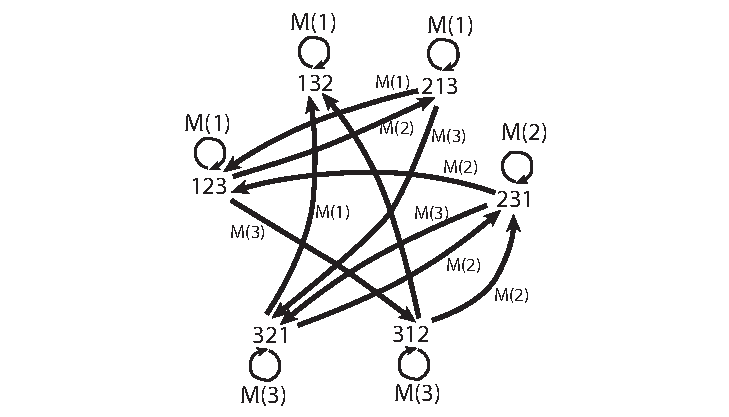
\includegraphics{pics/tr-markov}
\caption{Přechody mezi stavy}
\label{tr-markov}
\end{figure}


Tyto Markovovy řetězce jsou nerozložitelné a aperiodické a to znamená, že
existují asymptot. pravděpodobnosti, tj. pro seznam $\Pi$ je dána
pravděpodobnost ${\kappa}_{\Pi}$, že po provedení náhodné posloupnosti $P$ s
daným rozložením operací skončíme u seznamu $\Pi$.
\par

Pak očekávaný čas je $\sum_{\Pi}{\kappa}_{\Pi}\sum_{i}{\beta}_i\Pi(i)$, 
$\Pi(i)$ je pozice $i$ v seznamu $\Pi$.
\par
$p_1 = \sum_{\Pi}{\kappa}_{\Pi}\Pi(i)$ ... očekávaná pozice prvku $i$
\par
$\delta(j,i)$ = asmyptot. pst., že prvek $j$ je před $i$, pak platí \\
$$
\delta(j,i) = \sum\{\kappa_\Pi , \Pi\ seznam, \Pi(j) < \Pi(i)\}
$$

pak 
\begin{equation}
\begin{split}
p_i & = \sum_{\Pi}\kappa_\Pi\Pi(i) \\
& = \sum_{\Pi}\kappa_\Pi(1 + |{j, \Pi(j) < \Pi(i)|} \\
& = 1 + \sum{j,\Pi}\{\kappa_\Pi, \Pi(j) < \Pi(i)\} \\
& = 1 + \sum_{j}\delta(j,i) (1)
\end{split}
\end{equation}

Zkusíme $\delta(j,i)$ spočítat jiným způsobem: \\
Idea: jak se může stát, že ve výsledném seznamu je $j$ před $i$ ?
V posloupnosti $P$ existovala operace MEMBER($x$) a po ní se už nevyskytovala
operace MEMBER($i$) ani MEMBER($j$).
\par

Jaká je pravděpodobnost tohoto jevu ?
\begin{multline}
\beta_j\sum_{k=0}^{\infty}[1 - (\beta_i - \beta_j)]^k 
= \beta_j \frac{1}{1-(1-(\beta_i+\beta_j)} 
= \frac{\beta_j}{\beta_j+\beta_i} \stackrel{(1)}{=} 
1 + \sum_{\substack{j,i\\j \ne i}} \frac{\beta_j}{\beta_j+\beta_i}
\end{multline}

Očekávaný čas operace \mnote{jake operace ? XXX} je 
$$
\sum_{i} \beta_i p_i 
= \sum_{\substack{j,i\\j \ne i}} \frac{\beta_i\beta_j}{\beta_i+\beta_j}
$$

Předpokládejme, že $\beta_1 \geq \beta_2 \geq ... \geq \beta_n$ \\
pak nejrychlejší algoritmus na seznam $x_1 - x_2 - ... - x_n$ je klasický
algoritmus bez přemísťování prvků. Klasický algoritmus je takový
algoritmus, který předem ví, jaké jsou pravděpodobnosti
přístupu k jednotlivým prvkům a má předem seznam srovnaný 
sestupně podle těchto pravděpodobností.
\par
Očekávaný čas tohoto algoritmu je 

\begin{equation}
\begin{split}
\sum_{i=1}^{n}i\beta_i 
& = 1 + \sum_{i,j=1} 2\frac{\beta_j\beta_i}{\beta_i+\beta_j} \\
& \leq 1 + \sum_{\substack{i,j\\j<i}} 2\beta_i 
= 1 + \sum_{i=1}^{n} 2(i-1)\beta_i \\
& = 1 + 2\cdot\sum_{i}i\beta_i - 2\sum_{i}\beta_i \\
& = 2\sum_{i=1}^{n}i\beta_i - 1
\end{split}
\end{equation}

Platí
$$
\frac{\beta_j}{\beta_j+\beta_i} \leq 1
$$


% Splay stromy -------------------------------------------------------------

\section{Splay stromy}
% thanks to Jana Skotáková & Martin Malý za zápisky, přepsal Vladimír Kotal

% \mnote{částečně převzato z textů FIT VUTBR}

Splay strom (splay tree, rozvinutý strom) patří do kategorie 
adaptabilních datových struktur určených k vyhledávání. Má základní 
vlastnosti binárních vyhledávacích stromů - obsahuje ohodnocené prvky. 
Každému reprezentovanému prvku $s \in S$, kde $S \subseteq U$, 
($U$ je universum) je přiřazena váha.
\par
V průběhu operací nad touto strukturou se však mění její uspořádání 
ve prospěch celkového snížení časové složitosti.


\subsection{Operace SPLAY}

Základní operací je pro práci s těmito stromy je SPLAY($x$) - rozšíření, 
která zjistí, zda $x$ je reprezentován v dané množině. 
Pokud x leží v množině, algoritmus ho přemístí do kořene.

Když $x$ neleží v množině, pak algoritmus přemístí do kořene buď nejmenší
prvek větší než $x$ nebo největší prvek menší než $x$ (který leží v reprez.
množině)

Tento mechanismus 
se začíná od stanoveného uzlu, a postupnými rotacemi způsobuje, že 
stanovený uzel se stane kořenem stromu, při zachování vyhledávacích 
relací. Celkovým výsledkem je skutečnost, že často používané položky se 
hromadí v blízkosti kořene. Na rozdíl od BVS, jehož nejhorší případ pro 
degenerovaný (lineární) strom má složitost $O(N)$ a je složitost splay 
stromu pro "$k$" různých po sobě jdoucích operací $O(k*\log(N))$. Tato 
složitost není stanovena tradičním přístupem "nejhorší případ", který hledá 
nejnevýhodnější situaci izolované operace, ale metodou "amortizované 
analýzy" (amortized analysis), která hodnotí celou sekvenci různých 
operací. Některé z nich jsou delší, některé kratší než $\log(N)$, ale v 
průměru vychází složitost $O(ln(N))$.

Splay stromy představují jeden z příkladů adaptabilních datových 
struktur, jejichž vnitřní uspořádání se mění vlivem jako vedlejší jev 
operací nad těmoto strukturami. Mají dobrou tendenci vyvažovat stromovou 
strukturu a svou vlastností přibližovat často vyhledávané klíče kořeni 
se podobají adaptibilní lineární struktuře pro sekvenční vyhledávání, v 
níž se každý vyhledaný uzel vymění se svým levým předchůdcem. I ve 
stromové podobě si algoritmus zachovává jednoduchost a průhlednost. 


\subsection{Podporované operace}

MEMBER($x$,$T$), INSERT($x$,$T$), DELETE($x$,$T$), 
JOIN2($T_1$,$T_2$), JOIN3(x, $T_1$, $T_2$) 
(nebo asi taky JOIN3($T_1$, $x$, $T_2$)), SPLIT($x$), 
CHANGEWEIGHT($x$, $\triangle$).

\begin{itemize}
\item JOIN2($T_1$,$T_2$) \\
Předpokládá, že $\forall$ prvky reprezentované $T_1 < \forall$ prvky
reprezentované $T_2$, tj. $max T_1 < min T_2$.

Výsledný strom reprezentuje $T_1 \cup T_2$.

\item JOIN3($T_1$, $x$, $T_2$) \\
Předpokládá, že $\forall$ prvky reprezentované $T_1 < x < \forall$ prvky 
reprezentované $T_2$, tj. $max T_1 < x < min T_2$.

Výsledný strom reprezentuje $T_1 \cup T_2 \cup x$.


\item SPLIT($x$,$T$) \\
Výsledek: strom $T_1$ : $\forall$ prvky $\in T_1 < x$\\
	strom $T_2$: $\forall$ prvky $\in T_2 > x$\\
+ informace, zda $x$ ležel v reprezentované množině

\item CHANGEWEIGHT($x$, $\triangle$) \\
Zjistí, zda $x$ leží ve stromě a pokud ano, pak k jeho váze přičte
$\triangle$.
\end{itemize}


\subsection{Algoritmus MEMBER}

Mechanismus vyhledání (splay search), pracuje stejně jako u BVS, ale 
po vyhledání se aplikuje na vyhledaný uzel mechanismus Splay, jehož 
výsledkem je přesunutí uzlu na místo kořene. 

Viz algoritmus \ref{alg:splay.mem}

\begin{algorithm}[!htb]
\caption{MEMBER pro Splay stromy}
\label{alg:splay.mem}
\begin{algorithmic}
\STATE SPLAY(x, S)
\IF {x je reprezentován v kořeni}
  \STATE "$x$ je v $S$"
\ELSE 
  \STATE "$x$ není v $S$"
\ENDIF
\end{algorithmic}
\end{algorithm}

\subsection{Algoritmus JOIN2}

Viz algoritmus \ref{alg:splay.join2}

\begin{algorithm}[!htb]
\caption{JOIN2($T_1$,$T_2$)}
\label{alg:splay.join2}
\begin{algorithmic}
% oprava by M. Macok (nejmensi -> nejvetsi), argumenty SPLAY()
% oprava by T. Matousek - opracne
\STATE SPLAY($\infty$, $T_1$) // XXX (největší ?) nejmenší prvek \\
\STATE kořen $T_2$ bude pravý syn kořene $T_1$
\end{algorithmic}
\end{algorithm}

Operací SPLAY se z $T_1$ stane strom, kde pravý syn kořene bude list. 
Místo toho listu navěsíme strom $T_2$. \\
Pak budou v levém podstromu kořene tohoto nového stromu všechny prvky 
menší než hodnota v kořenu a v pravém všechny větší, což chceme.

\begin{figure}[!htb]
\centering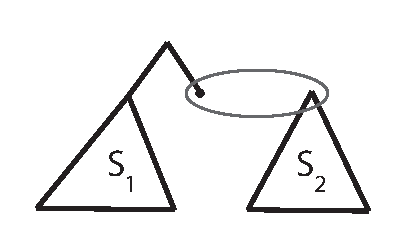
\includegraphics{pics/splay-join2}
\caption{JOIN2 pro splay stromy}
\label{splay-join2}
\end{figure}


\subsection{Algoritmus JOIN3}

Viz algoritmus \ref{alg:splay.join3}

\begin{algorithm}[!htb]
\caption{JOIN3($T_1$, x, $T_2$)}
\label{alg:splay.join3}
\begin{algorithmic}
\STATE vytvoříme vrchol $t$ reprezentující $x$
\STATE kořen $T_1$ je levý syn $t$ \\
\STATE kořen $T_2$ je pravý syn $t$
\end{algorithmic}
\end{algorithm}

Vytvoříme nový vrchol reprezentující $x$ a jeho synové budou $T_1$ -- levý,
$T_2$ -- pravý.

\begin{figure}[!htb]
\centering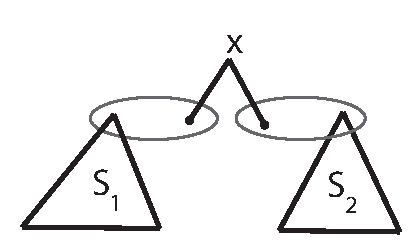
\includegraphics{pics/splay-join3}
\caption{JOIN3 pro splay stromy}
\label{splay-join3}
\end{figure}

\subsection{Algoritmus SPLIT}

Viz algoritmus \ref{alg:splay.split}

\begin{algorithm}[!htb]
\caption{SPLIT($x$,$T$)}
\label{alg:splay.split}
\begin{algorithmic}
%\STATE SPLAY(x)
%\IF {kořen T reprezentuje x}
%  \STATE $T_1$ podstrom levého syna kořene
%       \STATE $T_2$ podstrom pravého syna kořene
%       \STATE výstup $T_1$, $T_2$, x, $x \in S$
%  \ELSE
%       \IF {kořen T reprezentuje prvek $<$ x}
%          \STATE $T_2$ podstrom pravého syna kořene T
%	       \STATE $T_1 = T - T_2$
%	  \STATE T1 podstrom pravého syna kořene T
%	       \STATE $T_2 = T - T_1$
%       \ENDIF
%       \STATE výstup $T_1$, $T_2$, $x \in S$
%\ENDIF
\STATE SPLAY($x$)
\STATE $y$ = prvek reprezentovaný kořenem
\STATE $T_1$ = podstrom levého syna kořene
\STATE $T_2$ = podstrom pravého syna kořene
\IF {$y = x$}
  \STATE výstup $T_1$, $T_2$
  \STATE $x \in T$
\ELSIF {$y < x$}
  \STATE výstup $T \setminus T_2, T_2$
\ELSE
  \STATE výstup $T_1, T \setminus T_1$
\ENDIF
\STATE $x \not\in T$
\end{algorithmic}
\end{algorithm}

\mnote{zde chybi obrazek, ale celkem není pro pochopení potřeba :)}


\subsection{Algoritmus DELETE}

Mechanismus rušení uzlu (splay delete) je poněkud složitější. Uzel, 
který se má zrušit, se mechanismem splay přesune na pozici kořene. 
Zrušením kořene získáme 2 podstromy. Mechanismus splay se dále aplikuje 
na bezprostředního předchůdce a není-li tak následníka zrušeného uzlu 
(ve smyslu relace uspořádání - v průchodu inorder). Tím se tento uzel 
dostane do pozice kořene levého podstromu. Podle pravidel vyhledávacího 
stromu musí být všechny uzly levého podstromu menší než jeho kořen a 
všechny uzly pravého podstromu větší. Proto musí mít levý podstrom kořen 
vpravo volný a na toto místo se připojí pravý podstrom. Tento postup má 
symetrickou - levou versi. Operace "Splay Delete", rušící uzel D XXX je 
uvedena na obr.2.2. XXX
\par
Viz algoritmus \ref{alg:splay.delete}

\begin{algorithm}[!htb]
\caption{DELETE(x)}
\label{alg:splay.delete}
\begin{algorithmic}
\STATE SPLAY(x)
\IF {kořen reprezentuje x}
  \STATE $T_1$ je podstrom levého syna kořene T
       \STATE $T_2$ je podstrom pravého syna kořene T
       \STATE T $\leftarrow$ JOIN2($T_1$, $T_2$)
\ENDIF
\end{algorithmic}
\end{algorithm}

jiný zápis:
\begin{algorithmic}
\STATE $T_1, T_2 \leftarrow SPLIT(x, T)$
\STATE $T \leftarrow JOIN2(T_1, x, T_2)$
\end{algorithmic}

\subsection{Algoritmus INSERT}

Mechanismus vkládání (splay insert) vloží uzel jako list stejným 
způsobem jako BVS, ale potom se aplikuje na vložený uzel mechanismus 
"splay", který opět posune vložený uzel na pozici kořene. Operace
"Splay 
insert" uzlu s klíčem C XXX je uvedena na obr. \ref{splay-insert}.
\par


\begin{figure}[!htb]
\centering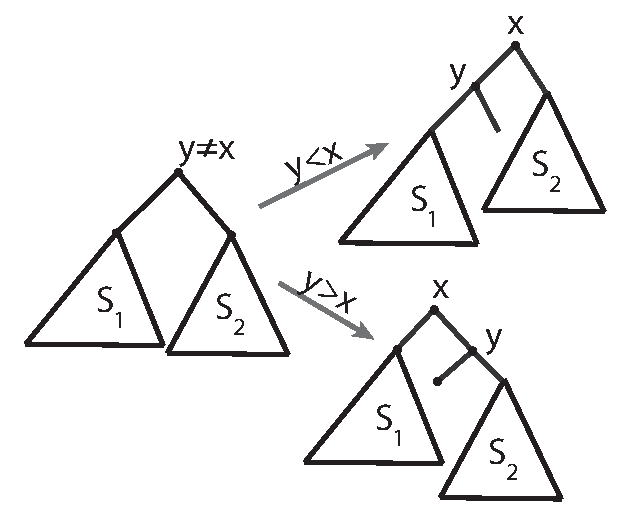
\includegraphics{pics/splay-insert}
\caption{INSERT(x) pro splay stromy}
\label{splay-insert}
\end{figure}


Viz algoritmus \ref{alg:splay.insert}

\begin{algorithm}[!htb]
\caption{INSERT(x)}
\label{alg:splay.insert}
\begin{algorithmic}
\STATE SPLAY(x)
\IF {kořen nereprezentuje x}
  \IF {kořen stromu reprez. prvek $<$ x}
          \STATE $T_2$ je podstrom pravého syna kořene
               \STATE $T_1$ = T - $T_2$ 
	  \ELSE 
	       \STATE T1 je podstrom levého syna kořene
	       \STATE $T_2$ = T - $T_1$
       \ENDIF
       \STATE JOIN3($T_1$, x, $T_2$)
\ENDIF
\end{algorithmic}
\end{algorithm}

jiný zápis:
\begin{algorithmic}
\STATE $T_1, T_2 \leftarrow SPLIT(x, T)$
\STATE $T \leftarrow JOIN3(T_1, x, T_2)$
\end{algorithmic}

\subsection{Algoritmus CHANGEWEIGHT}

Viz algoritmus \ref{alg:splay.chgw}

\begin{algorithm}[!htb]
\caption{CHANGEWEIGHT(x, $\triangle$)}
\label{alg:splay.chgw}

\begin{algorithmic}
\STATE SPLAY(x)
\IF {x je reprezentován v kořeni}
	\STATE k váze x přičti $\triangle$
\ENDIF
\end{algorithmic}
\end{algorithm}

Předpokládejme, že $w(x)$ je váha prvku a je to kladné celé číslo.
\par
$tw(x)$ - totální váha $x$, je to součet vah všech prvků v podstromě
určeném $x$.

\begin{priklad}
\mnote{chybí obrázek, tady je to nejake zmatene}
% XXX obr

$tw(a) = w(a) + w(b) + w(c)$ \\

$r(x)$ je $rank(x)$ \\
$r(x) = \lfloor \log tw(x) \rfloor$

$bal(konfigurace) = \sum \{ r(x) : x \in konfigurace \}$

Pro strom $T$ je $tw(x) = tw(\text{kořen }T)$ \\
	       $r(T) = r(\text{kořen }T)$
\end{priklad}

\begin{lemma}
Nechť $T$ je binární vyhledávací strom, $t$ je vnitřní vrchol a $u$,$v$ jsou
synové $t$. Pak $r(t) > min\{r(u), r(v)\} (r(list) = -\infty)$.
\end{lemma}

\begin{proof}
Předpokládejme, že $tw(u) \leq tw(v)$\\
$$
r(t) = \lfloor \log tw(t) \rfloor \geq \lfloor \log 2tw(u) \rfloor =
1 + \lfloor \log tw(u) \rfloor = 1 + r(u)
$$
\end{proof}

\subsection{Algoritmus SPLAY}

Volání algoritmu SPLAY se většinou zapisuje jako SPLAY($x$), kde explitictně
neuvádíme strom, na kterém je operace prováděna - to většinou vyplyne z
kontextu. Tam, kde je nutné uvést, na kterém stromě se operace SPLAY
provádí (např. v implementaci operace JOIN2, píšeme volání jako 
SPLAY($x$,$T$).

Viz algoritmus \ref{alg:splay.spl}

\begin{algorithm}[!htb]
\caption{SPLAY(x)}
\label{alg:splay.spl}
\begin{algorithmic}
\STATE SPLAY(x)
\STATE $t$ $\leftarrow$ kořen
\WHILE {$t$ není list a $t$ nereprezentuje $x$}
	\IF {$x < t$}
		\STATE $t$ $\leftarrow$ levý syn $t$
	\ELSE
		\STATE $t$ $\leftarrow$ pravý syn $t$
	\ENDIF
\ENDWHILE
\IF {$t$ je list}
	\STATE $t \leftarrow otec(t)$
\ENDIF
\WHILE {$t$ není kořen}
	\IF {$otec(t)$ je kořen}
	  \STATE rotace($t$, otec($t$))
	\ELSE
		\IF {otec($t$) i $t$ jsou oba leví (praví) synové}
		  \STATE rotace(otec($t$), děd($t$))
		  \STATE rotace($t$, otec($t$))
		\ELSE
		  \STATE dvojitá rotace($t$, otec($t$), děd($t$))
		\ENDIF
	\ENDIF
\ENDWHILE
\end{algorithmic}
\end{algorithm}

V algoritmu
SPLAY (algoritmus \ref{alg:splay.spl}) se používá jednoduché 
(obr. \ref{splay-rot}) a dvojité (obr. \ref{splay-dvojrot}) rotace.
Vrchol $t$ se po skončení operace SPLAY(x) dostane do kořene. Toho
dosáhneme tak, že v prvním cyklu najdeme vrchol $t$ reprezentující prvek
$x$, v druhém cyklu přesouváme vrchol $t$ do kořene.

\begin{figure}[!htb]
\centering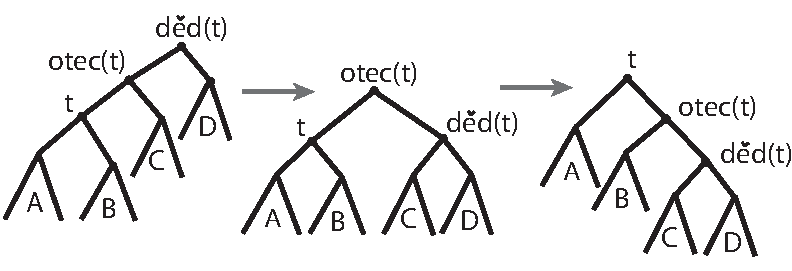
\includegraphics{pics/splay-rot}
\caption{Dvakrát jednoduchá rotace pro SPLAY($x$)}
\label{splay-rot}
\end{figure}

\begin{figure}[!htb]
\centering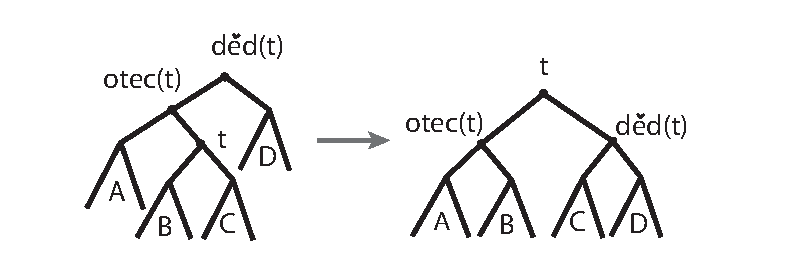
\includegraphics{pics/splay-dvojrot}
\caption{Dvojrotace pro SPLAY($x$)}
\label{splay-dvojrot}
\end{figure}


\subsection{Amortizovaná složitost SPLAY}

Budeme předpokládat, že $v(x) \geq 1$ pro každé $x$. \\
Totální váha $x = w(x)$, což je součet vah všech prvků v podstromu vrcholu
reprezentujícího $x$.
\par
Značíme $r(x) = \lfloor log_2 w(x)\rfloor = \text{rank vrcholu } x$
\par
Pro strom $T$: \\
$$w(T) = w(\text{kořen}(T)) \\
r(T) = r(\text{kořen}(T))$$
\par
bal(konfigurace) = součet ranků všech vrcholů v množinách tvořících
konfigurace
\par
Náš cíl : Budeme chtít ukázat, že amortizovaná složitost operací je
$O(\log\frac{w(T)}{v(x)})$, když $T$ reprezentuje $S$.
\par
Čas operace SPLAY = počet běhů druhého cyklu, který vrchol $t$ 
transportuje do kořene.


\begin{lemma}
\label{splay-pomlemma}
Pomocné lemma: Mějme vrchol $w$ ve stromě $T$ se syny $y_1$ a $y_2$ a
předpokládejme, že $y_1$, $y_2$ nejsou listy. Když $w$ reprezentuje $a$,
$y_r$ reprezentuje $b_i$ pro $i=1,2$, pak $rank(a) > min\{r(b_1),r(b_2)\}$
\end{lemma}

\begin{proof}
\begin{figure}[!htb]
\centering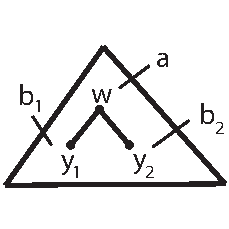
\includegraphics{pics/splay-lemma}
\caption{Pro důkaz pomocného lemmatu pro splay stromy}
\label{splay-lemma}
\end{figure}

Situaci lze vidět na obrázku \ref{splay-lemma}. 
\par
Zřejmě $r(a) \geq r(b_1)$ a $r(a) \geq r(b_2)$, tedy $r(b_1) \neq r(b_2) 
\Rightarrow r(a) > min\{r(b_1),r(b_2)\}$
\par
\begin{equation}
\begin{split}
r(a) 
& = \lfloor \log_2 w(a) \rfloor \geq \lfloor (w(b_1) + w(b_2)) \rfloor \\
& \geq \lfloor \log_2(2 - min\{w(b_1),w(b_2)\}) \\
& = 1 + \log_2 min\{w(b_1),w(b_2)\} \\
& = 1 + min\{w(b_1),w(b_2)\}
\end{split}
\end{equation}
\end{proof}

\begin{theorem}
Amortizovaná složitost operace SPLAY($x$,$T$) $\leq 3(r(T)-r(t)) + 1$, 
kde $t$ je vrchol, který transportujeme do kořene. $T$ je strom
reprezentující $S$.
(když $x$ je prvek reprez. množiny, pak $t$ reprezentuje $x$, jinak je to buď
největší nebo nejmenší prvek menší (větší) než $x$)
\end{theorem}

\begin{proof}
Označme $T_0$ původní strom, $T_i$ strom po $i$-tém běhu druhého cyklu 
v SPLAY a
předpokládejme, že druhý cyklus běží k-krát. (tj. $T_k$ je výsledný strom)
\par
Amortizovaná složitost (SPLAY($x$,$T$)) 
\mnote{$\text{``čas operace``} = k$}
\begin{equation}
\begin{split}
& = \text{čas operace} + bal(\text{výsledná konfigurace}) - 
bal(\text{původní konfigurace}) \\ 
& = k + bal(T_k) - bal(T_0) \\
& = \sum_{i=1}{k}(1 + bal(T_i) + bal(T_{i-1})
\end{split}
\end{equation}
\mnote{$balance = \sum \text{rank v }T_k$}

Označme $r_i$ rank ve stromě $T_i$, nechť $u_i$ je otec $t$ ve stromě
$T_i$ a když $u_i$ není kořen $T_i$, pak $v_i$ je otec $u_i$ v $T_i$.

\begin{itemize}
\item a)
$u_i$ je kořen: \\
chci odhadnout $1 + bal(T_i) - bal(T_{i-1})$ :
\begin{equation}
\begin{split}
& 1 + bal(T_i) - bal(T_{i-1}) \\
& = 1 + \sum_{z \text{ reprezentován v }T_i} r_i(z) + \sum_{z} r_{i-1}(z) \\
& = 1 + r_i(u_{i-1}) + r_i(t) - r_{i-1} - r_{i-1}(t) \\
& = 1 + r_i(u_{i-1}) - r_{i-1}(t) 
\leq 1 + 3(r_{i-1}(u_{i-1}) - r_{i-1}(t))
\end{split}
\end{equation}

\begin{figure}[!htb]
\centering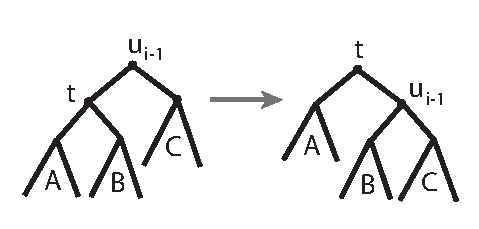
\includegraphics{pics/splay-amortproof1}
\caption{Pro důkaz amort. složitosti operace SPLAY}
\label{splay-amortproof1}
\end{figure}

Platí $r_i(t) = r_{i-1}(u_{i-1})$, protože stromy $A$,$B$,$C$ na obr.
\ref{splay-amortproof1} jsou stejné.
\par
Platí
$$
r_i(u_{i-1}) \leq r_{i-1}(u_{i-1}) 
$$
$$
r_{i-1}(u_{i-1}) \geq r_{i-1}(t)
$$

\item b)
  $u_{i-1}$ není kořen: 
  \begin{enumerate}
  \item $u_{i-1}$ je jiný syn v $T_{i-1}$ než $t$
  \item $u_{i-1}$ je stejný syn v $T_{i-1}$ jako $t$
  \end{enumerate}
\end{itemize}

\par
\begin{itemize}
\item ad b1) : \\
\begin{equation}
\begin{split}
& 1 + bal(T_i) - bal(T_{i-1} = \sum_{z}{} r_i(z) - \sum_{z}{} r_{i-1}(z) \\
& = 1 + r_i(t) - r_i(u_{i-1}) + r_i(v_{i-1}) - r_{i-1}(t) - r_i(u_{i-1}) -
	r_{i-1}(v_{i-1}) \\
& = 1 + r_i(u_{i-1}) + r_i(v_{i-1}) - r_{i-1}(t) - r_{i-1}(u_{i-1}) \\
& \leq 2(r_{i-1}(v_{i-1}) - r_{i-1}(t)) \\
& \leq 3(r_{i-1}(v_{i-1}) - r_{i-1}(t))
\end{split}
\end{equation}

První nerovnost v odvození platí, protože 
$1 + r_i(u_{i-1}) + r_i(v_{i-1}) = 2r_{i-1}(t) = 2r_{i-1}(v_{i-1})$.
\par
Amortizovaná složitost během cyklu: $\leq 3(r_i(v_{i-1}) - r_{i-1}(t))$

\item ad b2) : \\

$1 + bal(T_i) - bal(T_{i-1}) = ... 
= 1 + r_i(u_{i-1}) + r_i(v_{i-1}) - _{i-1}(t) - r_{i-1}(u_{i-1}) \leq$

  \begin{itemize}
  \item{$\alpha$} \\
    Předpoklad: $r_{i-1}(t) < r_i(v_{i-1})$ \\
    Pak platí: \\
    $\leq 1 + 2(r_{i-1}(v_{i-1}) - r_{i-1}(t)) 
    \leq 3(r_i(v_{i-1}) - r_{i-1}(t))$
  \item{$\beta$} \\
    Předpoklad: $r_{i-1}(t) = r_i(v_{i-1})$, $r_i(t) > r_i(v_{i-1})$ \\
    $... = 1 + r_i(u_{i-1}) + r_i(v_{i-1}) - r_{i-1}(t) - r_{i-1}(u_{i-1})
    \leq 2(2(r_{i-1}(v_{i-1}) - r_{i-1}(t))
    \leq 3(r_i(v_{i-1}) - r_{i-1}(t))$
  \item{$\gamma$} \\
    Předpoklad: $r_i(t) = r_i(v_{i-1}) - r_{i-1}(v_{i-1}) = r_{i-1}(t)$ \\
    Vím: $r_{i-1}(t) = r'(t) = r_{i-1}(v_{i-1}) = r'(u_{i-1}) 
    = r_i(t) = r_i(v_{i-1}) = r'(v_{i-1})$
    spor s lemmatem \ref{splay-pomlemma}.
    $\Rightarrow$ případ $\gamma$ nemůže nastat
  \end{itemize}

  Závěr pro b) : Amortizovaná složitost během cyklu 
  $\leq 3(r_i(v_{i-1}) - r_{i-1}(t))$

\end{itemize}

Vždy platí $r_i(v_{i-1}) = r_i(t)$ \\
\begin{equation}
\begin{split}
& \sum_{i=1}{k}(1 + bal(T_i) - bal(T_{i-1})) \\
& \leq \sum_{i=1}{k} 3(r_i(v_{i-1}) - r_{i-1}(t)) \\
& = 1 + 3(r_{k-1}(v_{k-1}) - r_0(t)) = 1 + 3(r_o(T) - r_0(t))
\end{split}
\end{equation}


%
% XXX toto je puvodni dukaz jsem napsal nekdy v 2003:
%
%rozdělíme podle akce, která se provádí ve while cyklu
%\begin{itemize}
%\item while cyklus provádí rotace
%
%$= 1 + r'(u) - r(v) \leq 1 + r(u) + r(v)$ \\
%$\leq 1 + 3(r(u) - r(v))$
%
%protože $x$ má v původním i novém stromě stejné prvky
%\mnote{nečitelné}
%$r(u) = r'(t)$ \\
%$r'(u) \leq r'() = r(u)$
%
%\par
%% b)
%\item while cyklus provádí dvojitou rotaci
%
%\mnote{tady chybi obr.}
%
%\begin{multline}
%\label{amort-dvojrotace}
%\text{Amortizovaná složitost této operace} \\
%\text{= čas operace + bal(nová konf.) - bal(původní konf.) =} \\
%= 1 + r'(u) - r(v) - r(u) - r(t)
%\end{multline}
%
%pro $x \neq t,u,v$ platí $r(x) = r'(x)$ \\
%$r(v) = r'(t)$
%
%\begin{itemize}
%  \item
%  \begin{multline}
%  r(v) > r(t), pak r'(u),r'(v) \leq r'(t) = r(v)\\
%  r(u) \geq r(t), 1 \leq r(v) - r(t) \stackrel{\text{ \ref{amort-dvojrotace}
%  }}{\leq} \\
%  r(v) - r(t) + 2r(u) - 2r(t) = 3(r(v) - r(t))
%  \end{multline}
%  
%  \item
%  r(v) = r(t), pak podle lemmatu $r'(t) > min\{r'(u), r'(v)\}$ plati \\
%  \begin{multline}
%  2r'(t) \geq r'(u) + r'(v) + 1 
%    \stackrel{\text{ \ref{amort-dvojrotace} }}{\leq} \\
%  2r(u) - 2(r(t) = 2(r(v) - r(t)) = (r(t) = 0) 3(r(u) - 3r(t))
%  \end{multline}
%  
%\end{itemize}
%\end{itemize}

\end{proof}




% -------------------------------------------------------------------------

\subsection{Amortizovaná složitost ostatních operací}

\begin{defn}
Amortizovaná složitost operace $SPLAY(x,T) \leq 1 + 3(r(T)-r(t))$, kde $t$
je prvek, který se přemístí do kořene.
\end{defn}

\par
Označme $t_{-}$ prvek ve stromě T, který reprezentuje největší prvek 
$\leq x$.
\par
Označme $t_{+}$ prvek ve stromě T, který reprezentuje nejmenší prvek 
$\geq x$.
\par
Když $x$ je reprezentováno $T$, pak $t_{-} - t_{+}$ je prvek reprezentující
$x$.
\par
Jednotlivé operace mají následující amortizované složitosti:

\begin{itemize}
\item $SPLAY(x,T) = O(\log\frac{w(T)}{min\{w(t_{-}),w(t_{+})\}})$ \\
\item $MEMBER(x,T) = O(\log\frac{w(T)}{min\{w(t_{-}),w(t_{+})\}})$ \\
\item $SPLIT(x,T) = O(\log\frac{w(T)}{min\{w(t_{-}),w(t_{+})\}})$ \\
\item $CHANGEWEIGHT(x, \triangle) = O(\log\frac{
w(T) - max\{\triangle,0\}}{min\{w(t_{-}),w(t_{+})\}
})$ \\
\item $JOIN3(T_1, x, T_2) = O(\log\frac{w(T_1)+w(T_2)+v(x)}{v(x)})$
\end{itemize}

Označme $t_{\infty}$ prvek v $T_1$, který reprezentuje největší prvek z
$T_1$. Pak amortizované složitosti pro zbývající operace jsou
následujicí:
\par

\begin{itemize}
\item $JOIN2(T_1,T_2) = O(\log\frac{w(T_1) + w(T_2)}{w(t_{\infty})})$ \\
\item $DELETE(x,T) = O(\log\frac{w(T)}{min\{w(t_{-}),w(t_{+}),w(t_{1}\}})$ \\
\end{itemize}

Prvek $t_1$ je prvek $T_1$, který reprezentuje v $T$ největší prvek $\leq x$.

\begin{itemize}
\item $INSERT(x,T) = O(\log\frac{w(T) + v(x)}{min\{w(t_{-}),w(t_{+})\}})$
\end{itemize}

% priklad pro SPLAY stromy ----------------------------------------------

\begin{priklad}
Mějme množinu $X={x_1,...,x_n}$ a pravděpodobnosti pro výskyt operace
MEMBER(x). Nechť $U$ je optimální binární vyhledávací strom. Nechť $T$ je
binární vyhledávací strom reprezentující $X$. $P$ je posloupnost operací
MEMBER(x) vyhovující daným pravděpodobnostem.
\par
Chceme aplikovat $P$ na strom $T$, kde pro implementaci použijeme strategii
SPLAY stromů.
\par
Srovnáme čas, který tato strategie vyžaduje s časem obvyklé implementace
MEMBER při aplikaci $P$ na $U$.
\par
Definujeme $v(x) = 3^{d-d(x)}$, kde d je hloubka stromu $U$ a $d(x)$ je
hloubka prvku v $U$ reprezentujícího prvek $x$.
\par
Spočítáme totální váhu prvku $x$:
$$w(x) = \sum_{i=0}{d-d(x)} 2^i3^{d-d(x)-i} 
\leq 3^{d-d(x)} \sum_{i=0}{d-d(x)} (\frac{2}{3})^i \leq 3^{d-d(x)+1}$$
\par
Pak platí: \\
$r(x) \leq d-d(x)+1$ \\
$r(T) \leq d+1$, (prvek v kořeni má hloubku $0$)
\par
Amortizovaná složitost operace MEMBER(x) 
$$\leq O(d(x)) = 
O(r(T)-r(x)) = O(d+1-d+d(x)-1) = O(d(x))$$
\par
Čas posloupnosti $P$ použité na strom $T$ a implementované strategií SPLAY 
$$= (\sum_{\text{operace v P}}{} \text{amortizovaná složitost operací v P}) +
bal(T) = O(\text{čas P pro strom U} + bal(T))$$
\par
$bal(T)$ je balance stromu $T$. 
$$bal(T) = \sum_{x \in X}{} r(x) = 
\sum_{x \in X}{} d+1 = O(x^2)$$
\par
$$\Rightarrow  O(\text{čas P pro strom U}) + bal(T) = 
O(\text{čas P pro U} + x^2)$$
\mnote{tady bylo ve vzorci něco jako $|x^2|$ (?)}
\par
Závěr: pro dlouhé posloupnosti snad téměř stejné jako opt. BVS.
\end{priklad}

% EOF

% ==========================================================================
% ==========================================================================
% prednaska DS 7.4.2003

\chapter{Haldy}

\begin{defn}
Haldy jsou stromov� struktury, kter� spl�uj� 
\begin{itemize}
\item lok�ln� podm�nku na uspo��d�n�
  - prvek reprezentuj�c� otce je men�� ne� prvek reprezentovan� synem
    apod.
% oprava by M. Macok:
% "strukturalni podminky" na stromy jsou podminky na tvar
% stromu (event. lesu), podle kterejch se ty haldy rozdelujou na Fib.,
% leftlist apod... neni tam nic o tom, jestli jsou synove vetsi/mensi
% nez otcove apod., od toho je tam ta prvni podminka...
\item struktur�ln� podm�nku na stromy, ze kter�ch jsou vytvo�en� 
\end{itemize}
\end{defn}

\begin{pozn}
Podle t�chto podm�nek se haldy rozd�luj� na Fibonacciho, Leftist,
d-regul�rn� apod. (mohou se li�it jak lok�ln�, tak struktur�ln� podm�nkou)
\end{pozn}

% --------------------------------------------------------------------------
\section{$d$-regul�rn� haldy}

\begin{defn}
d-regul�rn� halda, $d$ cel� ��slo $d \geq 2$ \\
Je to strom $T$ takov�, �e existuje jednozna�n� korespondence mezi vrcholy
strom� a prvky reprezentovan� mno�iny a plat�:
\begin{enumerate}
\item strom $T$ spl�uje struktur�ln� podm�nky:
  \begin{itemize}
    \item ka�d� vrchol s vyj�mkou nejv��e jednoho je bu� list nebo m� $d$ syn�
    \item ka�d� vrchol m� nejv��e $d$ syn�
    \item existuje o��slov�n� syn� ka�d�ho vrcholu tak, �e po o��slov�n�
  	  pr�chodem ���ky plat�: \\
	  kdy� vrchol nen� list, pak ka�d� vrchol s men��m ��slem m� $d$
	  syn�.
	  %\footnote{Tato podm�nka ��k� jin�mi slovy toto: V posledn�
	  %hladin� jsou v�echny uzly um�st�ny co mo�n� nejv�ce "vlevo",
	  %tzn. proch�z�me-li uzly p�edposledn� hladiny zleva doprava,
	  %nejprve m� n�kolik z nich (pop�. ��dn�) $d$ n�sledn�k�, pak m��e
	  %b�t (ale nemus�) jeden uzel s jedn�m n�sledn�kem a zb�vaj�c� 
	  %uzly p�edposledn� hladiny n�sledn�ky
	  %nemaj�. (parafr�ze z~\cite{Topfer}, str.~79)}.
  \end{itemize}
  \item podm�nku na lok�ln� uspo��d�n�: \\
	kdy� $x$ je prvek p�i�azen� vrcholu $t$, pak otci($t$) je p�i�azen
	prvek $\leq x$ pak po o��slov�n� pr�chodem do ���ky plat�:
	kdy� vrchol m� ��slo $i$, jeho synov� maj� ��sla
% oprava by M.Macok :
% strana 70, prvni syn vrcholu neni na pozici d(i-1)+1 ale ..+2
	$d(i-1)+2,d(i-1)+3,...,di+1$ a otec m� ��slo 
	$\lceil\frac{i-1}{d}\rceil$.
\end{enumerate}
\end{defn}

\begin{priklad}
P��klad 3-regul�rn� haldy je na obr�zku~\ref{XXX}.

\mnote{XXX chybi obr.}

Kdy� takto o��slovan� prvky d�me do pole, pak plat�: kdy� je vrchol na
$i$-t�m m�st�, ��sla syn� jsou $3(i-1)+2, 3i, 3i+1$
a otec je na $\lceil\frac{i-1}{3}\rceil$ m�st� v poli.
to vyu�ijeme pro implementaci polem - u�et��me m�sto.
\end{priklad}

\begin{pozn}
Nejpopul�rn�j�� jsou 2-reg. haldy, proto�e synov� i-t�ho vrcholu
jsou na m�stech $2(i-1)+2=2i, 2(i-1)+3=2i + 1$, otec je na
$\lceil\frac{i-1}{2}\rceil + 1 = \lceil\frac{i}{2}\rceil$. 
$\Rightarrow$ snadn� po��t�n� (bitov� posun)
\end{pozn}

\subsection{Algoritmus UP}

Operace UP($x$) srovn� haldu sm�rem nahoru.

\begin{algorithm}[!htb]
\caption{UP pro d-regul�rn� haldy}
\label{alg:heap.dreg.up}
\begin{algorithmic}
\STATE A: 
\IF {prvek reprezentovan� $x$ je $<$ prvek reprezentovan� otcem($x$)} 
  \STATE $x$ a otce($x$) vym�n�me 
  \STATE pokra�ujeme v A
\ENDIF
\end{algorithmic}
\end{algorithm}


\subsection{Algoritmus DOWN}

\begin{algorithm}[!htb]
\caption{DOWN pro d-regul�rn� haldy}
\label{alg:heap.dreg.down}
\begin{algorithmic}
\STATE A:
\IF {prvek reprezentovan� $x >$ prvek reprezentovan� n�kter�m synem $x$}
  \STATE vym�n�me $x$ a syna $x$, kter� reprezentuje nejmen�� prvek,
  \STATE pokra�ujeme v A
\ENDIF
\end{algorithmic}
\end{algorithm}

\begin{pozn}
Kdy� m� hlada hloubku $h$, pak UP($x$) vy�aduje �as $O(h)$, DOWN($x$) �as
$O(dh)$.
\end{pozn}

\subsection{Operace na hald�}

\subsubsection{INSERT}

\begin{algorithm}[!htb]
\caption{INSERT pro d-regul�rn� haldy}
\label{alg:heap.dreg.insert}
\begin{algorithmic}
\STATE p�id�me posledn� list $t$ reprezentuj�c� $x$
\STATE UP($t$)
\end{algorithmic}
\end{algorithm}

\subsubsection{MIN}

\begin{algorithm}[!htb]
\caption{MIN pro d-regul�rn� haldy}
\label{alg:heap.dreg.min}
\begin{algorithmic}
\STATE vr�t� prvek reprezentovan� v ko�eni
\end{algorithmic}
\end{algorithm}

\subsubsection{DELETEMIN}

viz algoritmus~\ref{alg:heap.dreg.deletemin}.

\begin{algorithm}[!htb]
\caption{DELETEMIN pro d-regul�rn� haldy}
\label{alg:heap.dreg.deletemin}
\begin{algorithmic}
\STATE prvek reprezentovan� posledn�m listem d�me do ko�ene
\STATE odstran�me posledn� list 
\STATE DOWN(ko�en)
\end{algorithmic}
\end{algorithm}

\subsubsection{DECREASEKEY$(x, \Delta)$}

Proveden� t�to operace p�edpokl�d�, �e mus�me zn�t polohu vrcholu $t$
reprezentuj�c�ho $x$, toto halda neumo��uje nal�zt. 

viz algoritmus~\ref{alg:heap.dreg.decrkey}.

\begin{algorithm}[!htb]
\caption{DECREASEKEY pro d-regul�rn� haldy}
\label{alg:heap.dreg.decrkey}
\begin{algorithmic}
\STATE zm�n�me uspo��d�n� v bod� $x$ 
\STATE UP($x$) mohl by b�t men�� ne� jeho otec, proto provedeme UP 
\end{algorithmic}
\end{algorithm}

\subsubsection{INCREASEKEY$(x, \Delta)$}

Mus�me zn�t polohu vrcholu $t$ reprezentuj�c�ho $x$, 
toto halda neumo��uje nal�zt. 
viz algoritmus~\ref{alg:heap.dreg.incrkey}.

\begin{algorithm}[!htb]
\caption{INCREASEKEY pro d-regul�rn� haldy}
\label{alg:heap.dreg.incrkey}
\begin{algorithmic}
\STATE zm�n�me uspo��d�n� v bod� $x$ 
\STATE DOWN($x$)
\end{algorithmic}
\end{algorithm}

\subsubsection{DELETE}

Mus�me zn�t polohu vrcholu $t$ reprezentuj�c�ho $x$, toto halda neumo��uje
nal�zt.
\par
Vezmeme prvek $y$ reprezentovan� posledn�m listem, odstran�me posledn� list,
prvek $t$, kter� reprezentoval $x$ bude reprezentovat $y$.


\begin{algorithm}[!htb]
\caption{DELETE pro d-regul�rn� haldy}
\label{alg:heap.dreg.delete}
\begin{algorithmic}
\IF {$y < x$} 
  \STATE UP($t$) else DOWN($t$) 
\ENDIF
\end{algorithmic}
\end{algorithm}

\subsection{Algoritmus MAKEHEAP}

D�na prost� posloupnost $x_1, x_2, ..., x_n$.
Chceme vytvo�it d-reg. haldu reprezentuj�c� mno�inu 
${ x_1, x_2, ..., x_n }$. Vezmeme "d-reg. strom" $T$ s vrcholy p�i�ad�me
prvky $x_1, x_2, ..., x_n$. Pro v�echny vrcholy, kter� nejsou listy podle
o��slov�n� v po�ad� od nejv�t��ho k nejmen��mu provedeme DOWN($t$).
\par

\mnote{chyb� obr�zek}
% XXX obr.

Invariant: v okam�iku, kdy prov�d�m DOWN($t$), tak vrcholy, kter�
reprezentuj�c� v�t�� prvky spl�uj� sm�rem dol� podm�nku 

\subsection{Slo�itost operac�}

V d-reg. hald� reprezentuj�c� n-prvkovou mno�inu implementace operac�
vy�aduje �asy dan� tabulkou:

\begin{center}
\begin{tabular}{|l|l|}
\hline
Operace & Slo�itost \\
\hline
MIN & O(1) \\
INSERT, DECREASEKEY & $O(log_d(n))$ \\
DELETEMIN, INCREASEKEY, DELETE & $O(d \cdot log_d(n))$ \\
\hline
\par
\end{tabular}
\end{center}

M�me vrchol v $i$-t� hladin� a "d-reg. strom" m� hloubku $h$. 
Kolik �asu pot�ebuje DOWN($t$) ?
Je to $O(d(h-1))$.
\par
Po�et vrchol� v $i$-t� hladin� je $di$. \\
�as MAKEHEAP je 
$O(\sum{i=0}{h-1} d^id(h-i)) = O(dS)$, kde 
$$
S = \sum{i=0}{h-1}d^i(h-i)
$$

Budeme po��tat 
\begin{multline}\bigparens
dS - S = \sum{i=0}{h-1}d^{i+1}(h-i) - \sum{i=0}{h-1}d^{i}(h-i) = \\
d^h - h + \sum{i=0}{h-1}d^{i}(h-i-(h-i-1)) = d^h - h\frac{d^h - 1}{d-1} \\
\Rightarrow S = \frac{d^h - h}{d-1} + d\frac{d^{h-1} - 1}{(d-1)^2}, 
h = log_d(n) \Rightarrow S \approx O(\frac{n}{d})
\end{multline}


\subsection{Dijkstr�v algoritmus}

K �emu jsou d-reg. haldy dobr� ? nap�. pro implementaci Dijkstrova
algoritmu.
\par

\begin{itemize}
\item[Vstup:] orientovan� graf $(V,E)$, fce $c:E \rightarrow R^+$, vrchol $z$
\item[V�stup:] $d(v)$, $v \in V$ \\
	$d(v)$ je d�lka nejkrat�� cesty ze $z$ do $v$ \\
\end{itemize}

\begin{algorithm}[!htb]
\caption{Dijkstr�v algoritmus pro d-regul�rn� haldy}
\label{alg:heaps.d-reg.dijkstra}
\begin{algorithmic}
\STATE $d(z) = 0, d(v) = \infty \forall v \in V, v \neq z, U = {z}$\\
\WHILE {$U \neq \emptyset$}
  \STATE vezmeme z $U$ prvek $u \in U$ s nejmen�� hodnotou $d(u)$,
    \STATE odstran�me ho z $U$.
  \FOR {$\forall(u,v) \in E$}
    \IF {$d(v) > d(u) + c(u,v)$} 
       \STATE $d(v) = d(u) + c(u,v)$ , v p�id�me do  $U$
    \ENDIF
  \ENDFOR
\ENDWHILE
\end{algorithmic}
\end{algorithm}
\par

$U$ reprezentujeme pomoc� d-reg. haldy. Pak �as Dijkstrova algoritmu je 
$$
O(|V| \cdot \text{�as na INSERT } + |V| \cdot 
\text{�as na DELETEMIN } + |E| \cdot \text{�as na DESCREASEKEY}) 
$$

Kdy� $d = 2$, pak to je $O(|E|log_2(|V|))$
\par
$d = max {\frac{|E|}{|V|}, 2}$, vyjde �as $O(|E|log_d(|V|))$ 
\par
Kdy� $\exists \epsilon$ , �e $|E| \geq c|V|^{1+\epsilon}$ pro n�jak� $c$,
pak �as je $O(|E|)$. (graf je dostate�n� hust�) \\
$|E| \geq c|V|\log^{\epsilon} |V|$ pro n�jak� $c$, $\epsilon$, pak �as je
$O(|E|\log log |V|)$.
\par


\subsection{Heapsort}

T��d�c� algoritmus Heapsort je dal�� aplikac� d-regul�rn�ch hald.

HEAPSORT - viz alg. \ref{alg:heaps.d-reg.heapsort} 

\begin{itemize}
% XXX odsadit vic doprava, aby nadpisy pro items nepresahovaly
\item[Vstup:] prost� posloupnost prvk� $x_1, x_2, ..., x_n$
\item[V�stup:] uspo��dan� psl. prvk� $x_1, x_2, ..., x_n$
\end{itemize}

\begin{algorithm}[!htb]
\caption{Heapsort pro d-regul�rn� haldy}
\label{alg:heaps.d-reg.heapsort}
\begin{algorithmic}
\STATE MAKEHEAP($x_1, x_2, ..., x_n$)
  \STATE i = 1
  \WHILE {$HEAP \neq \emptyset$}
    \STATE $x_1$ = MIN(HEAP)
    \STATE DELETEMIN(HEAP)
    \STATE i = i + 1
  \ENDWHILE
\end{algorithmic}
\end{algorithm}

\begin{pozn}
Optimum pro d-reg. haldy je n�kde mezi $d=6$ a $d=7$.
\end{pozn}

% --------------------------------------------------------------------------
\section{Leftist haldy}

\begin{defn}
M�jme bin�rn� strom a pro ka�d�ho syna m�me ur�eno, zda je lev� nebo
prav�. Pro vrchol v definujeme npl(v) jako d�lku nejkrat�� cesty z v do
vrcholu v podstromu v s nejv��e jedn�m synem. 

Bin�rn� strom je LEFTIST, kdy� 
\begin{itemize}
\item[a)] kdy� vrchol $v$ m� jednoho syna, pak je to lev� syn
\item[b)] kdy� vrchol $v$ m� dva syny, pak 
	$npl(\text{lev�ho syna}) \geq npl(\text{prav�ho syna})$
\end{itemize}
\end{defn}

\begin{defn}
Cesta $x_1, x_2, ..., x_n$ se naz�v� {\emph prav�}, kdy� $x_i$ je prav� syn
$x_{i-1}$ pro $i=2,3,...,n$ a $x_n$ nem� prav�ho syna.
\end{defn}


Vlastnosti: 
\begin{enumerate}
\item ka�d� podstrom leftist stromu je leftist 
\item d�lka prav� cesty z $\forall$ vrcholu $v$ je 
$\leq log(\text{po�et vrchol� v podstromu vrcholu } v)$
\end{enumerate}

\begin{defn}
Letist halda reprezentuj�c� mno�inu $S$ je leftist strom $T$ s $n$ vrcholy
takov�, �e existuje jednozna�n� korespondence mez prvky $S$ a vrcholy
$T$ takov�, �e $\forall$ prvek p�i�azen� vrcholu $v \geq$ prvek p�i�azen�
otci $v$.
\end{defn}

%\begin{pozn}
%Podobn� operaci JOIN v AVL stromech (ale...)
% - v AVL stromech je operace JOIN ???
%\mnote{XXX rozv�st}
%\end{pozn}

\subsection{MERGE}

Operace MERGE s argumenty $T_1, T_2$ p�edpokl�d�, �e 
$T_1, T_2$ reprezentuj� disjunktn� mno�iny $S_1, S_2$.
V�sledkem t�to operace je halda reprezentuj�c� $S_1 \cup S_2$.

Form�ln� z�pis viz algoritmus \ref{alg:heaps.leftist.merge}

\begin{algorithm}[!htb]
\caption{MERGE pro leftist haldy}
\label{alg:heaps.leftist.merge}
\begin{algorithmic}
\STATE MERGE($T_1$, $T_2$)
\IF {$T_1$ = 0}
  \STATE MERGE($T_1$, $T_2$) $\rightarrow T_2$ konec 
\ENDIF
\IF {$T_2$ = 0}
  \STATE MERGE($T_1$, $T_2$) $\rightarrow T_1$ konec 
\ENDIF
\IF {ko�en $T_2$ reprezentuje prvek $<$ prvek repr. ko�enem $T_1$}
  \STATE vym�n�me $T_1$ a $T_2$
\ENDIF
\STATE prav� syn ko�ene $T_1 \rightarrow$ MERGE($T_2$, podstrom prav�ho syna ko�ene $T_1$)
\IF {npl(lev�ho syna ko�ene $T_1$) $<$ npl(prav�ho syna ko�ene $T_1$)}
  \STATE prohod�m syny ko�ene $T_1$
\ENDIF
\STATE npl(ko�ene $T_1$) = npl(prav�ho syna ko�ene $T_1$) + 1
\STATE MERGE($T_1$, $T_2$) $\rightarrow T_1$ 
\end{algorithmic}
\end{algorithm}

\begin{pozn}
�asov� slo�itost operace MERGE v leftist hald�ch je $O(log(n_1+n_2))$, kde
$n_1, n_2$ jsou velikosti reprezentovan�ch mno�in.
\end{pozn}

\subsection{INSERT}

viz algoritmus \ref{alg:heaps.leftist.insert}

\begin{algorithm}[!htb]
\caption{INSERT pro leftist haldy}
\label{alg:heaps.leftist.insert}
\begin{algorithmic}
\STATE INSERT(x)
\STATE vytvo��me novou haldu $T_1$ reprezentuj�c� pouze prvek x
\STATE T $\leftarrow$ MERGE($T_1$, $T_2$)
\STATE DELETEMIN
\STATE $T_1 \leftarrow$ podstrom lev�ho syna ko�ene $T$
\STATE $T_2 \leftarrow$ podstrom prav�ho syna ko�ene $T$
\STATE $T$ $\leftarrow$ MERGE($T_1$, $T_2$)
\end{algorithmic}
\end{algorithm}

\begin{theorem}
Operace MIN v leftist hald�ch vy�aduje �as $O(1)$, operace MERGE, INSERT, a
DELETEMIN vy�aduj� �as $O(log n)$, kde $n$ je po�et prvk� ve v�sledn� hald�.
\end{theorem}

\begin{pozn}
% XXX obr.
\mnote{XXX obr.}
Pod�v�me se jak vypad� v�sledn� strom a pod�v�me se na vrcholy, se kter�mi
jsme n�co museli prov�d�t - tyto vrcholy le�� na {\emph prav� cest�}, 
tj. je jich omezen� po�et.
\end{pozn}

\subsection{DECREASEKEY}

viz algoritmus \ref{alg:heaps.leftist.decreasekey}

\begin{algorithm}[!htb]
\caption{DECREASEKEY pro leftist haldy}
\label{alg:heaps.leftist.decreasekey}
\begin{algorithmic}
\STATE DECREASEKEY($x$)
\STATE odtrhneme podstrom $T_1$ vrcholu $x$, $y$ $\rightarrow$ otec($x$)
\STATE $T_2 = T - T_1$
\STATE zmen��me ohodnocen� ko�ene stromu $T_1$
\IF {$y$ m� jen prav�ho syna}
  \STATE zm�n�me tohoto syna na lev�ho, $npl(y) = 0$
\ENDIF
\STATE $y \rightarrow otec(y)$
\WHILE {$npl(y) > min\{npl(\text{lev� syn }y), npl(\text{prav� syn }y)\} + 1$}
  \IF {$npl(\text{lev�ho syna }y) < npl(\text{prav�ho syna }y)$}
    \STATE prohod�me syny $y$
  \ENDIF
  \STATE $npl(y) = npl(\text{prav�ho syna }y) + 1$, $y \rightarrow otec(y)$
\ENDWHILE
\STATE $T \leftarrow$ MERGE($T_1$, $T_2$)
\end{algorithmic}
\end{algorithm}

\begin{pozn}
$npl$, kter� jsem musel p�episovat, je v�dycky prav� syn.
\end{pozn}

\begin{theorem}
Operace DECREASEKEY, INCREASEKEY a DELETE vy�aduj� v leftist
hald�ch �as $O(log n)$. ($n$ je po�et prvk� v�sledn� reprez. mno�iny)
\end{theorem}


% --------------------------------------------------------------------------
\section{Binomi�ln� haldy}

\begin{defn}
\emph{Binomi�ln� strom} $B_i$ je rekurzivn� definov�n jako strom 
sest�vaj�c� se z
ko�ene a jeho d�t� $B_0, B_1, ..., B_{i-1}$. Ka�d� strom m� \emph{vlastnost
haldy}, tj. pro ka�dou stromovou hranu plat� $\text{kl�� otce} \leq
\text{kl�� syna}$.
\end{defn}

\begin{defn}
\label{def.binomheap}
\emph{Binomi�ln� halda} je soubor strom� takov�ch, �e
\begin{itemize}
\item ka�d� strom je izomorfn� s n�jak�m $B_i$
\item ��dn� dva stromy nejsou izomorfn�
\item existuje jednozna�n� korespondence mezi vrcholy reprezentovan�
mno�iny a vrcholy strom� takov�, �e prvek odpov�daj�c� otci je men�� ne�
prvek odpov�daj�c� vrcholu.
\end{itemize}
\end{defn}

\begin{pozn}
Nej�ast�ji je binom. halda implementov�na jako pole ukazatel�, kde $i$-t�
ukazatel ukazuje na ko�en stromu $B_i$ nebo je NIL. To, jak dlouh� pole
budeme pot�ebovat, je kardin�ln� pro amortizovanu slo�itost. Bin�rn� z�pis
��sla $n$ m� d�lku $\lfloor log_2 n \rfloor$ $\Rightarrow$ stromy ��du
vy���ho ne� $\lfloor log_2 n \rfloor$ se nebudou vyskytovat. (jinak by m�l
graf v�ce ne� $n$ vrchol�)

Binomi�ln� stromy rostou exponenci�ln� spolu s ��dem. (proto funguje
amort. anal�za)
\end{pozn}

\begin{pozn}
Na binomi�ln� strom se m��eme d�vat i jinak: strom $B_i$ sest�v� ze 2
kopi� $B_{i-1}$ (viz obr. \ref{fig.heaps.binomial})
a z�sk� se z nich operac� zvanou \emph{spojen�}. 
Binomi�ln� haldy souvis� s binomi�ln�m rozvojem ��sel.
\end{pozn}

\begin{algorithm}[!htb]
\caption{Spojen� dvou binomi�ln�ch strom�}
\label{alg:heaps.binom.spoj}
\begin{algorithmic}
\STATE Spojeni($S_1$, $S_2$)
\STATE $S_1, S_2$ jsou stromy izomorfn� s $B_i$ pro n�jak� $i$
\IF {prvek reprezentovan� ko�enem $S_1 \leq$ prvek reprezentovan� ko�enem $S_2$}
  \STATE ko�en $S_2$ se stane dal��m synem ko�ene $S_1$
\ELSE
  \STATE ko�en $S_1$ se stane dal��m synem ko�ene $S_2$
\ENDIF
\end{algorithmic}
\end{algorithm}

\begin{figure}[!htb]
\centering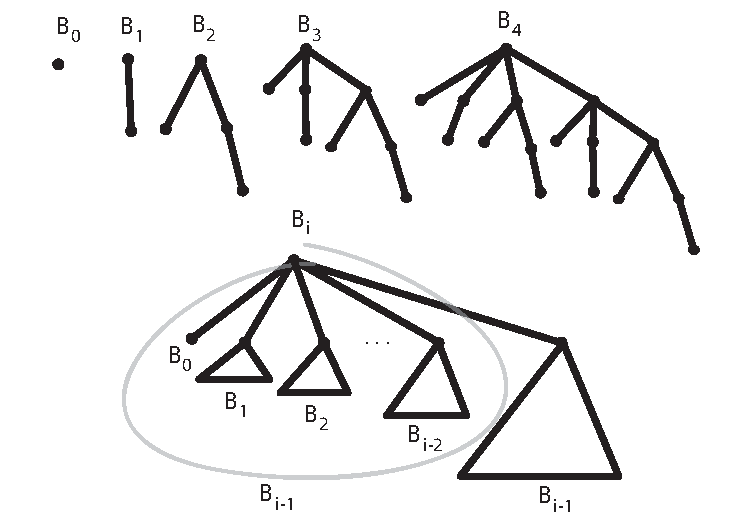
\includegraphics{pics/binheaps}
\caption{Binomi�ln� stromy}
\label{fig.heaps.binomial}
\end{figure}

\begin{tvrzeni}
Binomi�ln� halda je tvo�ena binomi�ln�mi stromy $B_i$, kter� maj� n�sleduj�c�
vlastnosti: 
\begin{itemize}
\item $B_i$ m� $2^i$ vrchol�
\item hloubka $B_i$ je i
\item ko�en $B_i$ m� i syn�
\item $\forall j < i$ existuje syn ko�ene $B_i$ takov�, �e 
  jeho podstrom je izomorfn� s $B_j$.
\end{itemize}
\end{tvrzeni}

\begin{proof}
indukc� p�es $i$ (element�rn�)
\end{proof}


\subsection{MERGE}

Algoritmus MERGE (viz algoritmus \ref{alg:heaps.binom.merge}) pracuje jako
"bin�rn� s��t�n�" - 2 stromy $B_i$ (= 2 jedni�ky v ��du $i$) slije do
$B{i-1}$ (= p�enos do $i+1$)

Pracuje v $O(\log_2 n)$ - nejvy��� mo�n� ��d je $\lfloor \log_2 n \rfloor$.
Toto je slo�itost v nejhor��m p��pad�.

Ukazatel MIN nov� haldy je nastaven na men�� z MIN($h_1$), MIN($h_2$) - to
zabere $O(1)$.


\begin{algorithm}[!htb]
\caption{MERGE pro binomi�ln� haldy}
\label{alg:heaps.binom.merge}
\begin{algorithmic}
\STATE MERGE($T_1$, $T_2$)
\STATE ($T_1, T_2$ binom. haldy velikosti $n_1,n_2$)
\STATE $P = 0, i = 0, T = 0$
\WHILE {$i \leq log(n_1 + n_2)$}
  \STATE $S_1$ je strom v $T_1$ izomorfn� s $H_i$ (pokud neexistuje, tak $S_1=0$)
  \STATE $S_1$ je strom v $T_1$ izomorfn� s $H_i$ (pokud neexistuje, tak $S_1=0$)
  % XXX \CASE
     \IF {$S_1, S_2$, P = 0}
       \STATE neprovedeme nic
     \ENDIF
     \IF {jeden strom z $S_1, S_2$, $P$ je nepr�zdn�} 
        \STATE vlo��m tento strom do $T$, $P=0$
     \ENDIF
     \IF {dva stromy z $S_1, S_2$, $P$ jsou nepr�zdn�}
       \STATE spoj�m tyto stromy a v�sledek vzlo��m do $P$
     \ENDIF
     \IF {v�echny stromy z $S_1, S_2$, $P$ jsou nepr�zdn�}
       \STATE vlo��m do $T$, spojen� $S_1, S_2$ vlo��m do $P$
     \ENDIF
  % \ENDCASE
  \STATE $i = i + 1$
\ENDWHILE
\end{algorithmic}
\end{algorithm}

\begin{pozn}
V algoritmu MERGE (viz algoritmus~\ref{alg:heaps.binom.merge}) 
odpov�d� $P$ p�enosu v bin�rn�m s��t�n�, $T$ je v�sledn� halda.
\end{pozn}

\subsection{MIN}

MIN($h$) - prohled�me prvky reprezentovan� ko�eny strom� a najdeme
nejmen��. V praxi je pro ka�dou haldu dr�en ukazatel, ukazuj�c� na ko�en
reprezentuj�c� nejmen�� prvek haldy. Tento ukazatel je obnovov�n p�i
operaci DELETE\_MIN.


\subsection{INSERT}

Operace INSERT($h$,$i$) se provede p��kazem MERGE($h$, MAKEHEAP($i$)).
Tato operace je analogick� s inkrementac� bin�rn�ho ��ta�e.

Dijkstr�v algoritmus prov�d� na za��tku $n$ operac� INSERT, n�m tedy nejde
o jednotliv� operace, ale o posloupnost INSERT�.

\begin{pozn}
INSERT je stejn� jako v leftist hald�ch.
\end{pozn}

\begin{theorem}
Amortizovan� slo�itost operace INSERT je $O(1)$.
\end{theorem}

\begin{proof}
Vyu�ijeme ��etn� metody: \\
Algoritmus INSERT udr�uje n�sleduj�c� invariant: \\
Ka�d� binom. strom v hald� m� na sv�m ��tu 1 jednotku. (Ten, kter�
p�est�v� b�t ko�enem, zaplat�, ten kdo vyhr�l, si 1 jednotku ponechal.)
P�i vytv��en� stromu ji zaplat� operace, kter� strom vytvo�ila: 
\begin{itemize}
  \item MAKEHEAP vytvo�� 1 strom $\Rightarrow$ zaplat� 1
  \item DELETE\_MIN vytvo�� $\leq log n$ strom� $\Rightarrow$ zaplat�
  	$\leq log n$
\end{itemize}
Pokud INSERT spust� kask�du sl�v�n�, pak je ka�d� slit� zaplaceno z ��tu
stromu, kter� dan�m slit�m zanikne. (jeho ko�en se stane synem)
\end{proof}


\subsection{DELETEMIN}

Operace DELETEMIN (viz algoritmus \ref{alg:heaps.binom.deletemin}) 
je provedena tak, �e ze stromu $B_k$, na kter� ukazuje
ukazatel MIN, utrhneme ko�en. T�m vzniknou nov� stromy $B_0, B_1, ...,
B_{k-1}$, ze kter�ch vytvo��me novou haldu, nastav�me pro ni ukazatel MIN
a zavol�me MERGE.

DELETEMIN pracuje v $O(log_2 n)$, proto�e $k \leq log_2 n$. Toto je
slo�itost v nejhor��m p��pad�.

\begin{algorithm}[!htb]
\caption{DELETEMIN pro binom. haldu}
\label{alg:heaps.binom.deletemin}
\begin{algorithmic}
\STATE DELETEMIN
\STATE prohled�n�m prvk� reprezentovan�ch ko�eny strom� naleznu strom $S$,
jeho� ko�en reprezentuje nejmen�� prvek
\STATE $T_1 = T \ {S}, T_2$ je tvo�en podstormy v�echn syn� ko�ene S
\STATE (tj. utrhnu ko�en a zbytek d�m do haldy) - 
	je to halda d�ky vlastnosti 4
\STATE $T \rightarrow$ MERGE($T_1, T_2$)
\end{algorithmic}
\end{algorithm}

\begin{pozn}
Operace DELETE se ned� rozumn� prov�st, museli bychom p�ebudovat cel�
strom.
\end{pozn}

\begin{theorem}
Operace MERGE, INSERT, MIN, DELETEMIN a DECREASEKEY vy�aduj� �as $O(log n)$.
Operace INCREASEKEY vy�aduje �as $O(log^2 n)$.
\end{theorem}

%\begin{pozn}
%S��t�n� v bin�rn�ch ��slech m� slo�itost $O(1)$.
%
%\begin{tabular}{|l|}
%\hline
%1 0 0 ... 0 \\
%\hline
%1 1 1 ... 1 \\
%\hline
%\end{tabular}
%\hspace{5mm}
%
%XXX amort. slo�. \\
%Neplat� n�co podobn�ho pro binom. stromy ? Ano, pro operaci INSERT.
%\end{pozn}

\begin{pozn}
MERGE zab�r� dost �asu - mus�me ho d�lat ?
\end{pozn}


\subsection{L�n� implementace binom. hald}

L�n� implementace vych�z� z toho, �e chceme operaci MERGE prov�d�t v �ase
$O(1)$.

Zm�n�me definici - vynech�me podm�nku 2 z definice \ref{def.binomheap}, 
tj. te� v na�� binom. hald� mohou b�t izomorfn� stromy. (i kdy� jen
do�asn�) Dal�� zm�na
spo��v� ve zm�n� reprezentace binomi�ln� haldy - haldu reprezentujeme
dvojit�m kruhov�m spojov�m seznamem p�es ko�eny strom�. (kruhov� spojov�
seznam umo��uje p�id�v�n� a odeb�rn� prvk� v �ase $O(1)$.)

Operaci MERGE($T_1, T_2$) pak m��eme prov�st konkatenac� seznam� $T_1$ a $T_2$.
Jenom to by nefungovalo, mus�me je�t� zm�nit operace MIN, DELETEMIN.

\begin{algorithm}[!htb]
\caption{DELETEMIN pro l�n� binom. haldy}
\label{alg:heaps.binom-line.min}
\begin{algorithmic}
\STATE MIN
\STATE p�i prohled�v�n� prvk� reprezentovan�ch ko�eny strom� se�ad�me
stromy do mno�in $Q_i$, $i=0,...,n$ , kde $Q_i$ je mno�ina v�ech strom� v
$T$ izomorfn�ch s $B_i$.
\STATE $i = 0, T = 0$
\WHILE {$\exists Q_i \neq 0$}
  \WHILE {$|Q_i| > 1$}
    \STATE vezmeme dva stromy z $Q_i$, spoj�me je, v�sledek d�me do $Q_{i+1}$
  \ENDWHILE
  \IF {$Q_i \neq 0$}
    \STATE strom z $Q_i$ d�m do $T$
  \ENDIF
  \STATE $i = i + 1$
\ENDWHILE
\end{algorithmic}
\end{algorithm}

DELETEMIN um�st� stromy po odtr�en� nejmen��ho prvku do odpov�daj�c�ch 
mno�in $Q_i$. (v mno�in� $Q_i$ jsou stromy izomorfn� s $B_i$)
Pot� provede \emph{konsolidaci} - uprav� haldu do podoby, kdy je ka�d� ��d
zastoupen nejv��e jedn�m stromem. 

Konsolidace b�� v $O(log n)$ plus vy�erp� ��ty strom�, kter� zaniknou p�i
sl�v�n�.

\begin{samepage}
Konsolidace prob�h� takto:
\begin{enumerate}
  \item vytvo��m pole d�lky $log n$, kter� je pr�zdn� 
  	$\Rightarrow$ $O(log n)$
  \item proch�z�m spojov� seznam vrchol� strom� v hald� 
  	a jeden strom za druh�m vyjmu a 
  	d�v�m do pole vytvo�en�ho v kroku 1, p�i�em� se v�dy provede 
	p��slu�n� slit�.
	\begin{itemize}
	  \item pokud strom zanikne, tak pr�ci zaplat�me z jeho ��tu
	  \item pokud strom nezanikne, tak pr�ci plat�me z ��tu
	  konsolidace $\rightarrow$ $O(log n)$
	\end{itemize}
  \item z pole vytvo��me spojov� seznam $\rightarrow$ $O(log n)$
\end{enumerate}
\end{samepage}

\begin{samepage}
DELETEMIN tedy pot�ebuje
\begin{itemize}
  \item $O(log n)$ do ��t� nov� vytvo�en�ch strom�
  \item $O(log n)$ na jejich zaveden� do spojov�ho seznamu
  \item $O(log n)$ na konsolidaci
\end{itemize}
\end{samepage}

P�i konsolidaci v�dy z�rove� vyhled�me nov� minimum.

\begin{theorem}
Operace MERGE a INSERT p�i l�n� implementaci vy�aduj� �as $O(1)$, operace
DELETEMIN a MIN vy�aduj� �as $O(\text{po�et strom� v hald�})$.
\end{theorem}

%\begin{pozn}
%$bal(\text{konfigurace}) = \text{po�et v�ech strom� ve v�ech hald�ch v
%konfiguraci}$
%\end{pozn}
%
%\subsubsection{Amort. slo�.}
%$\text{amort. slo�.} = \text{�as pro operaci} + 
%bal(\text{v�sledn� konfigurace}) - bal(\text{p�vodn� konfigurace})$

\vspace{5mm}

\begin{center}
\begin{tabular}{|l|l|}
\hline
Operace & Amort. slo�itost \\
\hline
MERGE & $O(1)$ \\
INSERT & $O(1)$ \\
MIN & $O(log n)$ \\
DELETEMIN & $O(log n)$ \\
\hline
\end{tabular}
\tabcaption{Amortizovan� slo�itost pro l�n� binomi�ln� haldy}
\label{tab:binheaps.lazy.complexity}
\end{center}

% \subsection{Zobecn�n� binomi�ln� haldy}

% XXX
% \mnote{p�edn�elo se to tento rok (2004) v�bec ?}

% --------------------------------------------------------------------------
\section{Fibonacciho haldy}

Fibonacciho haldy vych�zej� z binomi�ln�ch hald, form�ln� se li�� v podstat�
pouze t�m, �e v hald� povol�me i jin� stromy ne� binomi�ln�. Toto n�m
umo�n� implementaci operace DECREASE\_KEY, kter� nebyla v binomi�ln�ch
hald�ch p�i zachov�n� slo�itosti ostatn�ch operac� mo�n�.

��d uzlu a stromu je definov�n jako u binomi�ln�ch hald. Sl�v�n� se
prov�d� pouze mezi stromy stejn�ho ��du.

\subsection{MERGE, INSERT, EXTRACT\_MIN}

Implementace operac� MERGE($h_1$,$h_2$), INSERT($h$,$i$), EXTRACT\_MIN($h$) 
je stejn� jako u binomi�ln�ch hald v "l�n�" verzi.

\subsection{DECREASE\_KEY}

DECREASE\_KEY prov�d� sn��en� hodnoty kl��e pro dan� prvek. To se d�je za
cenu p��tomnosti jin�ch ne� binomi�ln�ch strom� v hald�.

\begin{algorithm}[!htb]
\caption{DECREASE\_KEY pro Fibonacciho haldy}
\label{alg:heap.fib.decrease_key}
DECREASE\_KEY($h$,$i$,$\delta$)
\begin{enumerate}
  \item sn���m kl�� prvku $i$ o $\delta$
  \item podstrom i s ko�enem $i$ od��zneme a jako samostatn� strom ho
        zavedeme haldy (tj. za�ad�m do spojov�ho seznamu ko�en� strom� v
	hald�) $\Rightarrow$ $O(1)$
  \item Abychom udr�eli stromy dostate�n� "ko�at�"\footnote{nechceme 
  	stromy typu "smet�k" - tj. takov�ch, kter� sest�vaj� pouze 
	z ko�ene a jeho syn�, kter� jsou z�rove� listy}
  	tak od ka�d�ho vrcholu $x$ mohou b�t od��znuti nejv��e 2
  	synov� $\Rightarrow$ po od��znut� 2. syna je od��znut i s�m vrchol $x$.
\end{enumerate}
\end{algorithm}

\begin{figure} 
\centering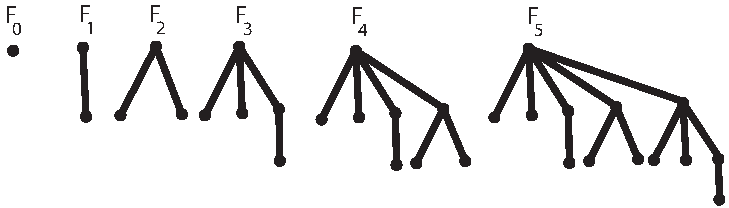
\includegraphics{pics/fibheaps}
\caption{Po�ty vrchol� strom� $F_0, F_1, ...$ tvo�� Fibonacciho
posloupnost.}
\label{fig:heaps.fib.pocty.vrcholu}
\end{figure}

\begin{pozn}
P�esto�e jedna operace DECREASE\_KEY m��e vyvolat kask�du �ez�, je jej�
amortizovan� slo�itost $O(1)$.
\end{pozn}

\begin{pozn}
Pomoc� \emph{��etn� metody}\footnote{Pro definici ��etn� metody viz
p�edn�ky ze "\emph{Slo�itosti a NP �plnosti}".}
dok�eme, �e to plat�: \\
P�i od�ez�v�n� syna vrcholu $x$ zaplat� operace DECREASE\_KEY
\begin{samepage}
\begin{itemize}
  \item 2 jednotky na ��et $x$
  \item 1 jednotku na ��et vznikl�ho stromu
  \item 1 jednotku za pr�ci (od��znut� a za�azen�)
\end{itemize}
\end{samepage}

P�i od��znut� druh�ho syna jsou na ��tu vrcholu $x$ 4 jednotky
$\Rightarrow$ mohu zopakovat body 1) - 3).
\end{pozn}

\begin{theorem}
\label{heaps.fib.theorem}
Nejvy��� ��d stromu ve Fibonacciho hald� je $\lfloor log_\varphi n \rfloor =
\Theta(log_2 n)$ pro n�jak� $\varphi > 1$.
\end{theorem}

\begin{lemma}
\label{heaps.fib.lemma}
Nech� $x$ je vrchol a $y_1, ..., y_m$ jeho synov� v po�ad�, v jak�m byli k
$x$ sliti. Potom $\forall \in {1,...,m}$ je ��d $y_i$ aspo� $i-2$.
\end{lemma}

\begin{proof}
V okam�iku, kdy byl $y_i$ slit pod $x$, m�l $x$ ��d $\geq i-1$.
($y_1,...,y_{i-1}$ ji� v t� chv�li byli synov� $x$)
V tomto okam�iku byl tak� ��d $y_{i-1} \geq i-1$. (sl�v�me pouze stromy
stejn�ho ��du) Od t� doby mohl $y_i$ ztratit nejv��e jednoho syna, jinak
by byl s�m od��znut a p�estal by b�t synem $x$. $\Rightarrow$ $y_i$ m� ��d
$\geq i-2$. 
\end{proof}

\begin{proof}
Dokazujeme v�tu \ref{heaps.fib.theorem}, kter� jin�mi slovy ��k�: 
Strom ��du $i$ ve
Fibonacciho hald� m� velikost alespo� $\varphi^i$ pro n�jak� $\varphi >
1$.

Nech� $F_j$ je nejmen�� mo�n� (tj. m� o�ezan� podstromy na max. mo�nou
�rove� - byl z nich od��znut 1 syn) strom ��du $j$ spl�uj�c� tvrzen� lemma
\ref{heaps.fib.lemma} a nech� $|F_j| = f_j$. Pak

\begin{enumerate}
  \item $F_i$ vznikne "slit�m" $F_{i-1}$ a $F_{i-2}$ $\Rightarrow$ 
  	$f_i = f_{i-1} + f_{i-2}$
  \item $f_i \geq \varphi^i$, kde 
  	$\varphi = \frac{1+\sqrt 5}{2} \approx 1.618$ ... zlat� �ez
\end{enumerate}

\begin{itemize}
  \item[ad 1)] 
  viz obr.~\ref{fig:heaps.fib.proof}

  \begin{figure} 
  \centering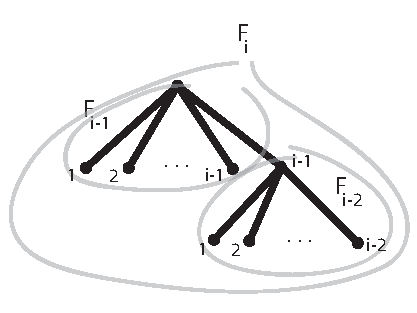
\includegraphics{pics/fibheap}
  \caption{K d�kazu v�ty \ref{heaps.fib.theorem}}
  \label{fig:heaps.fib.proof}
  \end{figure}

  Slit� je nep�esn� term�n - sl�v�me pouze stromy stejn�ho ��du.
  $F_{i-2}$ je v�sledek DECREASE\_KEY. (t�m se strom "oholil") U��znu
  posledn�ho syna, pod kter�m je nejv�t�� podstrom (abych dostal nejmen��
  mo�n� podstrom)

  \item[ad 2)]
  $\varphi$ je klad� ko�en rovnice $x^2 - x - 1 = 0$ \\
  neboli plat� $\varphi^2 = \varphi + 1$, $\varphi = \frac{1+\sqrt 5}{2}
  \approx 1.618$ \\
  dok�eme indukc�: 
    \begin{itemize}
      \item i = 0 : $f_0 = 1 \geq \varphi^0 = 1$
      \item i = 1 : $f_1 = 2 \geq \varphi^1 = 1.618$
      \item induk�n� krok: IP: $f_i \geq \varphi^i$, $f_{i+1} \geq
      \varphi^{i+1}$ \\
        $f_{i+2} = f_{i+1} + f_i \geq \varphi^{i+1} + \varphi^i =
	\varphi^i(\varphi + 1) = \varphi^{i+2}$
    \end{itemize}
\end{itemize}
\end{proof}



% ==========================================================================
% Součást skript na Datové struktury. Viz main.tex
\markright{$ $Id$ $}
% přepsal Vladimír Kotal

\chapter{Dynamizace}

V~uspořádaném poli umíme rychle vyhledávat, ale přidat prvky znamená
celé ho přebudovat. Ve~srůstajícím hašování zase nešly prvky mazat,
ve~velmi komprimovaných trie ani přidávat, ani mazat. V~této kapitole
ukážeme obecnou metodu, jak tyto problémy řešit, podobnou přístupu u
binomiálních hald.
\par
Takové struktuře, která neumožňuje vkládání (operace INSERT) ani mazání 
(operace DELETE) prvků budeme říkat
\emph{statická struktura}. Chceme vytvořit takovou reprezentaci, která
bude využívat výhod statické struktury, ale zároveň umožní operace INSERT
a DELETE.
\par
K tomu se dopracujeme postupně. 
Nejdříve provedeme \emph{semidynamizaci}, 
která umožní (v nové reprezentaci původní množiny) operaci INSERT, 
pak \emph{dynamizaci}, která přidá operaci DELETE. 



% --------------------------------------------------------------------------
\section{Zobecněný vyhledávací problém}

\begin{defn}
\emph{Vyhledávací problém} je funkce $f: U_1 \times 2^{U_2} \to U_3$, kde
$U_1$, $U_2$ a $U_3$ jsou univerza.
\end{defn}
\begin{defn}
\emph{Řešení vyhledávacího problému} pro $x \in U_1, A \subseteq U_2$
je nalezení hodnoty $f(x, A)$.
\end{defn}

\begin{pozn}
Chceme najít strukturu, která reprezentuje A a algoritmus, který pro vstup
$x \in U_1$ spočítá $f(x, A)$. Takové struktuře se říká 
\emph{statická struktura} pro vyhledávací problém.
\end{pozn}

\begin{priklad}
\begin{description}
\item[Klasický vyhledávací problém:]
	
	$U_1 = U_2 = U$, univerzum prvků; \\
	$U_3 = \{0, 1\}, A \subseteq U_2$ 

	$f(x, A) =
	\begin{cases}
	0& \text{když } x \notin A\\
	1& \text{když } x \in A
	\end{cases}$
	(rozložitelný)
\item[Euklidovská vzdálenost bodů v rovině:]

	$U_1 = U_2 = $ euklidovská rovina; 
	$U_3 = \mathbb{R}^+$; 
	$f(x, A) = dist(x,A$ vzdálenost bodu $x \in U_1$ od množiny $A$.
	(rozložitelný, $\oplus$ ... operace min)
\item{Nalezení předchůdce}
	$U_1 = U_2 = U_3$ 
	pro $x \in U_1$ a $A \subseteq U_!$ a je $f(x,U_!)$ je největší 
		prvek $A \leq x$
	(rozložitelný, je potřeba disjunkce)
\item[Příslušnost ke konvexnímu obalu]

	$U_1 = U_2 = $ rovina; 
	$U_3 = \{0, 1\}$;

	\begin{figure}[!htb]
	\centering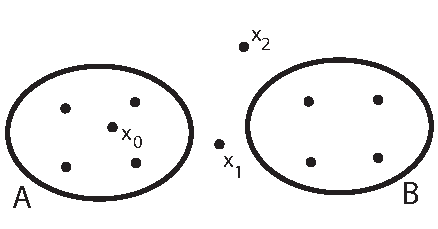
\includegraphics{pics/convex-envel}
	\caption{Konvexní obal}
	\label{convex-envel}
	\end{figure}

	\(f(x, A) =
	\begin{cases}
	0& \text{když $x$ nepatří do konvexního obalu $A$}\\
	1& \text{když $x$ patří do konvexního obalu $A$}
	\end{cases}\)
	(není rozložitelný problém)
\end{description}
\end{priklad}


\subsection{Operace INSERT a DELETE}

Pro množinu $A \subseteq U_2$ a pro statickou strukturu {\cal S}
řešící vyhledávací problémf pro $x \in U_2$.
\par
\begin{itemize}
\item INSERT($x$,$A$) - vybudování struktury řešící vyhledávací problém pro množinu
$A \cup \{x\}$
\item DELETE($x$,$A$) - vytvoření struktury řešící vyhl. problém pro množinu 
$A - \{x\}$
\end{itemize}

\begin{pozn}
Ze statické struktury chce vytovořit dynamickou (dynamizace). INSERT je
obvykle jednodušší než DELETE, na ten budeme potřebovat dodatečné
předpoklady.
\end{pozn}

Nároky na dynamizaci
\begin{itemize}
\item chceme aby se $f(x,A)$ v nové struktuře spočítalo přibližně 
  stejně rychle jako v původní struktuře
\item když vytvoření původní struktury pro $n$ prvnkovou množinu trvalo
  $t$, pak operace INSERT by přibližně měla vyžadovat čas $t/n$.
\end{itemize}

\begin{defn}
Vyhledávací problém je \emph{rozložitelný}, když
existuje operace $\oplus$ spočitatelná v konstantním čase a platí:
když $x \in U_1$ a $A$ a $B$ jsou disjunktní podmnožiny $U_2$, pak
\[
	f(x, A \cup B) = f(x, A) \oplus f(x, B).
\]
\end{defn}

\begin{pozn}
Z výše uvedených příkladů není rozložitelným problémem příslušnost ke
konvexnímu obalu, ostatní vyhledávací problémy jsou rozložitelné.
\end{pozn}

\newcommand{\staticka }{\ensuremath{\mathcal{S}}}
\newcommand{\dynamicka}{\ensuremath{\mathcal{D}}}


\begin{defn}
Nechť $f$ je rozložitelný vyhledávací problém a $\staticka$ je
``statická'' datová struktura, která ho řeší. Neboli $\staticka$ je
tvořena pro pevnou množinu $A \subseteq U_2$ a obsahuje operaci, která
pro vstup $x$ počítá $f(x, A)$.

Popíšeme důležité parametry $\staticka$: nechť $n = |A|$, označme
\begin{align*}
Q_\staticka(n) & = \text{čas potřebný pro výpočet $f(x,A)$}\\
S_\staticka(n) & = \text{paměť potřebná pro vybudování \staticka}\\
P_\staticka(n) & = \text{čas potřebný pro vybudování \staticka}
\end{align*}
\end{defn}

% ------------------------------------------------------------------------
\section{Semi-dynamizace}

Semi-dynamizace umožní operaci INSERT nad novou reprezentací původní
množiny. Tato reprezentace bude využívat statické struktury. Nejprve
provedeme "základní" semidynamizaci, poté ji vylepšíme pro INSERT se
složitostí v nejhorším případě. Vylepšení bude vyžadovat jiný rozklad
původní množiny a algoritmus INSERT (viz
algoritmus~\ref{alg:semidyn.insert.vylepseny}) 
bude složitější.

\begin{theorem}
Máme rozložitelný vyhled. problém $f$ a máme pro něj statickou strukturu,
která ho řeší v čase $Q(n)$, vyžaduje $S(n)$ paměti a vytvoří se v čase
$P(n)$,
kde $Q(n), \frac{P(n)}{n}, \frac{S(n)}{n}$ jsou neklesající funkce. Pak
existuje semidynamická dat. struktura $D$, řešící $f$ v čase
$O(Q(n)\log n)$ vyžadující $O(S(n))$ paměti a umožňující INSERT s 
amort. složitostí
$O(\frac{P(n)}{n} \cdot\log n)$.
\end{theorem}

\begin{proof}
Budeme předpokládat, že $Q_\staticka(n)$, $S_\staticka(n)/n$ a
$P_\staticka(n)/n$ jsou neklesající funkce.

Máme množinu $A$ a vytvoříme pro ni novou strukturu $D$.
Nechť $A_i \subseteq A$ taková, že buď $|A_i| = 2^i$ nebo $A_i = \emptyset$ \\
$A_i \cap A_j = \emptyset {\text pro } i \neq j$.
$\bigcup A_i = A$

Platí $A_i \neq \emptyset$ právě když $(i+1)$-ní bit v dvojkovém rozvoji čísla
$|A|$ je 1.

Chceme navrhnout strukturu, která by uměla
\begin{enumerate}
\item Pro $x \in U_1$ a pevné $A \subseteq U_2$ rychle spočítat $f(x, A)$.
\item Pro $A$ a $y \in U_2$ rychle vytvořit strukturu pro $A \cup \{y\}$.
\end{enumerate}

Mějme $A_0, A_1, \cdots$ takové, že
\begin{enumerate}
\item $A_i \cap A_j = \emptyset$ pro $i \neq j$
\item buď $A_i = \emptyset$ nebo $|A_i| = 2^i$ 
\item $\bigcup_i A_i = A$ 
\end{enumerate}

Nová struktura \dynamicka\ reprezentující $A$ je potom
\begin{itemize}
% \item XXX Seznam statických struktur pro $A_i \neq \emptyset$, $\staticka_i$
\item nějaká dynamická struktura reprezentující A
(např. (a,b)-strom, červeno-černý strom, AVL-strom)
% \item XXX Vyhledávací strom reprezentující $A$
\item Pro každé $A_i \neq \emptyset$ máme S strukturu reprezentující $A_i$.
\item Pro každé $A_i \neq \emptyset$ seznam prvků v $A_i$; prvky
těchto seznamů jsou projpojeny s odpovídajícími prvky ve stromě.
\end{itemize}

Jak v nové struktuře spočítáme $f(x,A)$ ? \\
Pro každou $A_i \neq \emptyset$ spočítáme $f(x,A_i)$ a pomocí operace
$\oplus$ pak spočítáme $f(x,A)$.

\begin{pozn}
Platí, že když $A_i \neq \emptyset$, pak 
$i \leq \lceil log_2|A| \rceil$
\mnote{XXX jak ma vypadat tento vzorec ?}
čas, který je potřeba v nové struktuře na výpočet $f(x,A)$
\end{pozn}

\begin{multline}
log_2|A| + \sum_{i=0}^{log|A|}Q(2^i) \leq log|A| + \sum_{i=0}^{log|A|}Q(|A|)
= log|A|(Q(|A|) + 1)
\end{multline}

\begin{pozn}
První nerovnost plyne z toho, že $Q(n)$ je nerostoucí funkce. 
V dalších důkazech pro $S$ a $P$ se využívá opět této vlastnosti pro
$\frac{S(n)}{n}$ a $\frac{P(n)}{n}$.
\end{pozn}

$log_2(|A|)$ - vyhodnocení $f(x,A)$ z $f(x,A_i), i=0,1,...$
\par

Tedy algoritmus potřebuje $O(log|A| Q(|A|))$ času
když $Q(n) = \Theta(n^\epsilon) pro \epsilon > 0$, pak platí, že nová
struktura pro výpočet $f$ potřebuje
\begin{equation}
\begin{split}
& log|A| + \sum_{i=0}^{log n}Q(2^i)  \\
& = |A| + \sum_{i=0}^{log |A|}
\frac{S(2^i)}{2^i} 2^i \leq |A| + \sum_{i=0}^{log |A|} \frac{S(|A|)}{|A|} 2^i \\
& = |A| - \frac{S(|A|)}{|A|} 2^i = |A| -
\frac{S(|A|)}{|A|}(\sum_{i=0}^{log |A|} 2^i) \\
& = O(S(|A|))
\end{split}
\end{equation}

\subsection{INSERT}


\begin{algorithm}[!htb]
\caption{INSERT pro semidynamizaci (rozklad $A$ na množiny $A_i$)}
\label{alg:semidyn.insert}
\begin{algorithmic}
\STATE INSERT(x)
\IF {$x \not\in A$} 
  \STATE nalezneme nejmenší $j$, že $A_j = \emptyset$
\ENDIF
\STATE $A_j = \{x\} \cup \bigcup{i<j} A_i, A_i = \emptyset$ pro $i<j$
\STATE vytvoříme strukturu $S$ spojový seznam pro $A_j$
\STATE $x$ přidáme do reprezentace $A$.
\end{algorithmic}
\end{algorithm}


Kdy se buduje znovu (tedy podruhé) $S$ struktura pro $A_j$ (měřeno počtem
INSERTů) ?
\begin{enumerate}
\item musí se naplnit všechny $A_i$ pro i<j 
to je $2^j-1$ úspěšných INSERTů (ty, které přidaly prvek)
\item provede se úspěšný INSERT, který vyprázdní $A_i$ pro $i \leq j$
\item znovu se musí naplnit $A_i$ tj. $2^j-1$ úspěšných INSERTů
\item daší úspešný INSERT vytvoří teprve S strukturu pro $A_j$
\end{enumerate}

tj. $2^j -1 + 1 + 2^j -1 + 1 = 2 \cdot 2^j = 2^{j+1}$ úspěšných INSERTů.

Amortizovaný čas operace INSERT je 
$$
log |A| + \sum_{i=0}^{log |A|} \frac{P(2^j)}{2^{j+1}} \leq
log |A| + \sum_{i=0}^{log |A|} \frac{P|A|}{|A|} = 
O(log |A| \cdot \frac{P|A|}{|A|})
$$

\end{proof}

\begin{theorem}
Máme rozložitelný vyhledávací problém $f$ a máme pro něj statickou strukturu,
která ho řeší v čase $Q(n)$, vyžaduje $S(n)$ paměti a vytvoří se v čase
$P(n)$,
$kde Q(n), \frac{P(n)}{n}, \frac{S(n)}{n}$ jsou neklesající funkce. Pak
existuje semidynamická dat. struktura $D$, řešící $f$ v čase
$O(Q(n)\log n)$ vyžadující $O(S(n))$ paměti a umožňující INSERT se
složitostí
$O(\frac{P(n)}{n} \cdot\log n)$.
\end{theorem}

% ------------------------------------------------------------------------

\subsection{INSERT se složitostí v nejhorším případě}

Následuje konstrukce takové semidynamické struktury, která bude podporovat
INSERT se složitostí v nejhorším případě.

\begin{pozn}
Pokud $\frac{P(n)}{n} = \Theta(n^\varepsilon)$ pro $\varepsilon > 0$, pak
amortizovaný čas pro operaci INSERT bude $O(\frac{P|A|}{|A|})$.
\end{pozn}

Máme množinu $A$ \\
budeme mít roklad $A$ na disjunktní množiny $A_{i,j}, i=0,1,..., j \in
{0,1,...,k_j}$, kde $k_j \in {0,1,2}$. \\
$|A_{i,j}| = 2^i$ a platí: \\
když $A_{i,0}$ existuje pro $i > 0$, pak existují $A_{i-1,0}, A_{i-1,1}$.
\par

Struktura: 
\begin{enumerate}
\item reprezentace $A$ (pomocí (a,b)-stromů, červeno-černých stromů, ...)
\item $\forall$ existující $A_{i,j}$ je $S$ struktura reprezentující
$A_{i,j}$ 
\item $\forall$ existující $A_{i,j}$ je spojový seznam reprezentující
$A_{i,j}$
\item když $A_{i,0}$ a $A_{i,1}$ existují pro nějaké i, pak je 
"rozpracovaná" $S$ struktura pro množinu $A_{i-1,k_i+1} = A{i,0} \cup
A_{i,1}$.
tj. bylo provedeno několik kroků pro její vytvoření, ale není dokončena.
\end{enumerate}


% nasleduje prednaska z 12.5.2003, prepsal Vladimír Kotal


$A \subseteq U_2, i_0 \in N$ \\
$\forall i = 0,1,...,i_0$ je dáno $j_i \in {0,1,2}$ takové, že $j_i > 0$
když $i < i_0$. \\
$\forall i = 0,1,...,i_0$ a $\forall j = 0,1,...,j_i$ je $A_{i,j} \in A$
taková, že $|A_{i,j}| < 2^i$.

\begin{defn}
${ A_{i,j}, i=0,1,...,i_0, j=1,2,...,j_i }$ je rozklad $A$.
\end{defn}

Pro každé $A_{i,j}$ je dána $S$ struktura reprezentující $A_{i,j}$ a spojový
seznam prvků z $A_{i,j}$, navíc dána dat. struktura reprezentující A.
Když $A_{i,1}$ existuje, pak je rozpracovaná S struktura pro
$A_{i+1,j_{i+1}+1} = A_{1,0} \cup A_{i,1}$.

\begin{pozn}
Struktura je rozpracovaná, jestliže bylo provedeno několik kroků
pro postaverní $S$ struktury, ale ještě není dokončena.
\end{pozn}

- toto je definice nové semidynamické struktury.

Paměťové nároky
\begin{equation}
\begin{split}
& |A| + \sum_{i=0}^{log |A|} 4S(2^i) \\
& = |A| + \sum_{i=0}^{log |A|} \frac{S(2^i)}{2^i}2^i \leq 
|A| + 4 \sum_{i=0}^{log |A|} \frac{S(|A|)}{|A|}2^i \\
& = |A| + \frac{4S(|A|)}{|A|} (\sum 2^i) = |A| + 4S(|A|) \\
& = O(S(|A|))
\end{split}
\end{equation}

\begin{pozn}
$|A|$ - paměť pro pom. struktury  \\
$\sum_{i=0}^{log |A|} 4S(2^i)$ - paměť potřebná na S struktury
\end{pozn}

Algoritmus pro výpočet : \\
spočítáme $f(x,A_{i,j})$ pro každou $A_{i,j}$ a pomocí operace $\oplus$
spočítáme $f(x,A)$. 

Čas potřebný pro výpočet $A$
\begin{multline}
\sum_{i=0}^{log |A|} 3Q(2^i) + 3\log |A| \leq 
3\sum_{i=0}^{log |A|} Q(|A|) + 3\log |A| = 
3Q(|A|)log |A| = O(Q(|A|)\log |A|)
\end{multline}

Platí: $Q(n) \geq n^{\epsilon}$ pro nějaké $\epsilon$, pak čas potřebný pro
výpočet $f$ je $O(Q(N))$.

INSERT(x) viz alg.~\ref{alg:semidyn.insert}

%\begin{algorithm}[!htb]
%\caption{Operace INSERT pro semidynamizaci}
%\label{alg:semidy.insert}
%\begin{algorithmic}
%\STATE když $x \notin A$ jinak provedeme:
%  \STATE vytvoříme S strukturu pro $A_{0,j_i+1} = \{x\}$ (zvětšíme $j_0$ o 1)
%  \IF {$j_o$ je liché}
%      \STATE pak provedeme 1.krok pro vytvoření S struktury
%      \STATE pro množinu $A_{1,j_1 + \lceil \frac{j_0}{2} \rceil} = A_{0,j_0 - 1}
%      \cup A_{0,j_0}$
%  \ENDIF
%  \STATE pro $i = 1,2,...,i_0+1$ v roustoucím pořadí:
%  \IF {S je rozpracovaná struktura pro $A_{i,j_i+1}$}
%    \STATE provedeme dalších $\frac{P(2^i)}{2^i}$ kroků pro její vybudování
%  \ENDIF
%  \STATE když jsme dobudovali S strukturu pro $A_{i,j_i+1}$, zvětšíme $j_i$ o 1
%  \STATE zrušíme $A_{i-1,0} \cup A_{i-1,1}$, zmenšíme $j_i$ o 2 a $A_{i-1,j}$ přepíšeme
%  na $A_{i-1,j_i+2}$.
%  \IF {$j_i$ liché} 
%    \STATE provedeme 1.krok pro vytvoření Q struktury pro
%    \STATE množinu $A_{1,j_i+1 + \lceil \frac{j_i}{2}} = A_{i,j_i} \cup A_{i,j_i-1}$.
%  \ENDIF
%\end{algorithmic}
%\end{algorithm}


\begin{algorithm}[!htb]
\caption{INSERT pro semidynamizaci (rozklad $A$ na $A_{i,j}$)}
\label{alg:semidyn.insert.vylepseny}
\begin{algorithmic}
\STATE INSERT(x)
\IF{$x \not\in A$}
  \STATE postavíme S-strukturu pro množinu $A_{0,j_0}={x}$
  \STATE $j_0$++
  \STATE $i=1$
  \WHILE{$j[i]>0$} 
    \IF{S-struktura pro $A_{i,j_i-1}$ není dostavěna}
      \STATE provedeme dalších $P(2^i)/2^i$ kroků pro vystavění 
      	S-stry pro $A_{i,j_i-1}$
      \IF{S-stra pro $A_{i,j_i-1}$ je dostavěna}
        \STATE $A_{i-1,0}=A_{i-1,2}$
        \STATE $A_{i-1,1}=A_{i-1,3}$
        \IF{$i-1>0$} 
          \STATE // na všech úrovních kromě 0-té, dojde k tom, že $j_i=5$
	  \STATE // tj. S-struktura pro $A_{i,4}$ je rozestavěna
          \STATE // poprvé k tomu dojde při 10. INSERTu, takže trpělivost
	  \STATE $A_{i-1,2}=A_{i-1,4}$
	\ENDIF
        \STATE $j_{i-1}=j_{i-1}-2$
        \STATE $A_{i,j_i}=A_{i-1,0} + A_{i-1,1}$
        \STATE provedeme první krok pro vystavění S-stry pro A[i,j[i]]
        \STATE $j_i$++
      \ENDIF
    \ENDIF
    \STATE $i++$
  \ENDWHILE

  \IF{$j[i-1] > 1$ a S-struktury pro $A_{i-1,0}$ a $A_{i-1,1}$ jsou dostavěny}
    \STATE $A_{i,0}=A_{i-1,0} + A_{i-1,1}$
    \STATE provedeme první krok pro vystavění S-struktury pro $A_{i,0}$
    \STATE $j_i$++
  \ENDIF
\ENDIF
\end{algorithmic}
\end{algorithm}

\mnote{Alg. INSERT pro semidyn. byl ověřen doktorem Koubkem}

\begin{pozn}
Může stát, že se vytvoří nová množina $A[i,j(i)]$, pak $j(i)$ má hodnotu
5, tj. musí se po dokončení struktury $A[i+1,j(i+1)-1]$ zmenšit o dvě
hodnoty $A(i,2)$, $A(i,3)$ a i $A(i,4)$ (nestačí jen pro první dvě hodnoty).
\end{pozn}

Čas pro INSERT(x) je \\
\begin{multline}
log |A| + \sum_{i=0}^{log |A|} (\frac{P(2^i)}{2^i} + 1) = 
2log |A| + \sum_{i=0}^{log |A|} \frac{2P(|A|)}{|A|} = \\
2log |A| + \frac{2P(|A|)}{|A|} \sum_{i=0}^{log |A|} 1 = 
2log |A| \frac{2P(|A|)}{|A|} log |A| = O(\frac{2P(|A|)}{|A|} log |A|)
\end{multline}

$log |A|$ - čas pro zjištění zda $x \in A$ \\

Když $\frac{P(n)}{n} \geq n^{\varepsilon}$ pro $\varepsilon > 0$, pak INSERT
vyžaduje čas $O(\frac{P(n)}{n})$.

\par
\begin{priklad}
XXX
\par
\vspace{5mm}

\begin{tabular}{|l|l|l|}
\hline
INSERT($x_1$) & INSERT($x_2$) & INSERT($x_3$) \\
\hline
$A_{0,0} = \{x_1\}$ & $A_{0,0} = \{x_1\}$ & $A_{0,0} = \{x_1\}$ \\
 & $A_{0,1} = \{x_2\}$ & $A_{0,1} = \{x_2\}$ \\
 & 1. krok pro $A_{1,0} = \{x_1,x_2\}$ & $A_{0,2} = \{x_3\}$ \\
 & & $\frac{P(2)}{2}$ kroků pro $A_{1,0} = \{x_1,x_2\}$ \\
 % \vspace{1mm}
\hline
INSERT($x_4$) & INSERT($x_5$) & INSERT($x_6$) \\
\hline
% XXX prvni dva radky skrtneme 
% prepsat skrtani poradne ze zapisku
$A_{0,0} = \{x_1\}$ & $A_{0,0} = \{x_3\}$ & $A_{0,0} = \{x_3\}$ \\
$A_{0,1} = \{x_2\}$ & $A_{0,1} = \{x_4\}$ & $A_{0,1} = \{x_4\}$ \\
$A_{0,2} = \{x_3\} \rightarrow A_{0,0} = \{x_3\}$ &
$A_{0,2} = \{x_5\}$ &
$A_{0,2} = \{x_5\} \rightarrow A_{0,0} = \{x_5\}$ \\
$A_{0,3} = \{x_4\} \rightarrow A_{0,1} = \{x_4\}$ &
$A_{1,0} = \{x_1,x_2\}$ &
$A_{0,3} = \{x_6\} \rightarrow A_{0,1} = \{x_6\}$ \\
dokončíme $A_{1,0} = \{x_1,x_2\}$ &
$\frac{P(2)}{2}$ kroků pro $A_{1,1} = \{x_3,x_4\}$ &
$A_{1,0} = \{x_1,x_2\}$ \\
1. krok pro $A_{1,1} = \{x_3,x_4\}$ & &
dokončeno $A_{1,1} = \{x_3,x_4\}$ \\
& & 1. krok pro $A_{1,2} = \{x_5,x_6\}$  \\
& & 1. krok pro $A_{2,0} = \{x_1,x_2,x_3,x_4\}$ \\
& & $\frac{P(4)}{4}$ kroků \\
% \vspace{1mm}
\hline
\end{tabular}

\end{priklad}

\begin{theorem}
Nechť $S$ je statická struktura pro rozložitelný vyhledávací problém $f$
a nechť $K$ je "hladká" funkce. Pak existuje semidynamická struktura $D$
založená na rozkladu určeném funkcí $K$, tak že platí: \\
když $K=O(log n)$, pak čas pro vyhledání je $O(K Q(n))$ \\
			  pro INSERT je $O(K(n) n^{\frac{1}{K(n)}}
			  \frac{P(n)}{n})$ \\
Když $K = \Omega(log(n))$, pak platí: \\
čas pro vyhledání je $O(K(n)) Q(n))$ \\
Pro INSERT je $O(\frac{log(n)}{log \frac{K(n)}{log(n)} }
\frac{P(n)}{n})$.
\end{theorem}

\begin{proof}
viz \cite{mehlhorn-overmars}.
\end{proof}

% dynamizace ----------------------------------------------------------

\section{Dynamizace}

Potřebujeme, aby struktura $S$ připouštěla falešný DELETE (prvek pouze
škrtneme, ale zůstane tam. falešný - čas. ani paměťové nároky se nezlepší
ani nezhorší)

\begin{defn}
\emph{Falešný DELETE} je operace, která vyškrtne prvek z množiny - tj. umožní
počítat $f(x,A-\{a\})$ (kde a je vyškrtnutý prvek) tak, že časové nároky
budou stejné jako když nebyl žádný prvek vyškrtnut.
\end{defn}

Budeme předpokládat, že čas pro falešný DELETE je $O(n)$, kde $n$ je velikost
původní reprezentované množiny.

\subsection{Reprezentace množiny A}

Rozložíme $A$ na disjunktní množiny $A_j, j=0,1,...,log|A|+3$
takové, že buď $A_j = \emptyset$ nebo $2^{j-3} < |A_j| \leq 2^j$.
\par
každá množina $A_j$ bude reprezentována strukturou, která původně (když
nebyly vyškrtnuté žádné prvky) měla velikost $\leq 2^j$.
\par
Dále $\forall A_j \neq \emptyset$ bude dán spojový seznam prvků v $A_j$.
\par
Bude dána datová reprezentace množiny $A$. Pro každý prvek a v spojovém
seznamu množiny $A_j$ bude dán ukazatel na prvek a  v dat. struktuře
reprezentující A a naopak. Pro každý prvek v dat. struktuře repr. $A$ je dán
ukazatel na prvek a v odpovídajícím spojovém seznamu.

\subsection{Paměťové nároky}

\begin{multline}
|A| + \sum_{i=0}^{log|A|+3} S(2^i) = |A| + \sum \frac{S(2^i)}{2^i} 2^i
\leq |A| + \sum_{i=0}^{log|A|+3} \frac{S(8|A|)}{8|A|} 2^i = \\
|A| + \frac{S(8|A|)}{8|A|} 2^i = |A| + \frac{S(8|A|)}{8|A|} \sum 2^i = 
|A| + S(8|A|) = O(S(8|A|))
\end{multline}
\par

$|A|$ - pomocné struktury \\
suma - paměť pro $S$ struktury
\par
Závěr: Když $S$ je omezená polynomem, pak paměťové nároky jsou $O(S(n))$.
Pokud $S$ je superpolynomiální, pak paměť. nároky jsou $O(S(8n))$
(a platí $S(n) = o(S(8n))$)
\par

Výpočet $f$: \\
spočítáme $f(x,A_j)$ a pomocí operace $\oplus$ spočítáme $f(x,A)$.

\subsection{Čas pro výpočet $f$}

$log(n) + \sum_{i=0}^{log|A|+3} Q(2^i) = log(n) + \sum Q(8|A|) =
O(Q(8|A|) log|A|)$.
\par

Závěr: čas na výpočet $f$ je
$\Biggl\{$
\begin{tabular}{ll}
když $Q$ je subpolynomiální & $O(Q(n)log(n))$ \\
polynomiální & $O(Q(n))$ \\
superplynomiální & $O(Q(8n))$ \\
\end{tabular}

% zde začíná poslední přednáška ze šk.r.2002/2003
% thanks to Jana Skotaková za zapůjčení, přepsal Vladimír Kotal

INSERT(x) viz alg. \ref{alg:dynam.insert_f}

\begin{algorithm}[!htb]
\caption{Operace INSERT (f)}
\label{alg:dynam.insert_f}
\begin{algorithmic}
\IF {$x \not \in A$}
  \STATE nalezneme nejmenší j takové, že $|\bigcup i \leq j A_i| < 2^j$
\STATE položíme $A_j = \bigcup{i\leq j}A_i \cup \{x\}$
\STATE $A_i = \emptyset pro i < j$
\STATE vytvoříme S-strukturu a spojový seznam pro $A_j$ (x přidáme do
struktury reprezentující A a přidáme požadované ukazatele)
\ENDIF  
\end{algorithmic}
\end{algorithm}

\par
Pozorování:\\
Když vytváříme při INSERTu S-strukturu pro $A_j$, pak $2^{j-1} < |A_j|
\leq 2^j$. \\
(když toto neplatí, pak pro $j-1$ je splněna nerovnost $|\bigcup{i<j-1} A_i|
< 2^{j-1}$ a to je spor s minimalitou $j$.
\par

% viz poznamky/datstr_054.jpg
DELETE(x) viz alg. \ref{alg:dynam.delete_f}

\begin{algorithm}[!htb]
\caption{Operace INSERT (f)}
\label{alg:dynam.delete_f}
\begin{algorithmic}
\IF {$x \not \in A$}
  \STATE odstraníme x ze struktury pro A
  \STATE nalezneme j takové, že $x \in A_j$ (budeme znát přímo místo x v seznamu
  pro $A_j$)
  \IF {$|A_j| = 1$}
    \STATE smažeme $A_j$ (odpovídající S-strukturu 
% tady to snad pokracuje     
     a spojový seznam) $\rightarrow A_j = \emptyset$
  \ENDIF
  \IF {$|A_j| > 1$ a zároveň $|A_j| > 2^{j-3} + 1$}
    \STATE na $S$ strukturu pro $A_j$ provedeme falešný DELETE($x$), $x$ smažeme
    ze spojového seznamu pro $A_j \rightarrow A_j = A_j - \{x\}$
  \ENDIF  
  \IF {$|A_j| > 1$ a zároveň $|A_j| = 2^{j-3} + 1$}
    \IF {$A_{j-1} = \emptyset$}
       \STATE $A_{j-1} = A_{j-1} - \{x\}, A_j = \emptyset$
       \STATE vybudujeme novou S-strukturu pro $A_{j-1}$
       ($x$ odstraníme ze spojového seznamu pro $A_{j-1} - 1$)
% \mnote{XXX tady nevím jestli nemá být jenom $A_{j-1}$}
    \ENDIF
    \IF {$A_{j-1} = \emptyset$ a zároveň $|A_{j-1}| > 2^{j-2}$}
      \STATE vyměním $A_j a A_{j-1}$
      \STATE z $A_{j-1}$ odstraníme x a vytvoříme novou S-strukturu pro
      $A_{j-1}$ (původní struktura mohla mít až $2^j$ prvků)
    \ENDIF
    \IF {$A_{j-1} = \emptyset$ a zároveň $|A_{j-1}| \leq 2^{j-2}$}
      \STATE $B = (A_j \cup A_{j-1}) - \{x\}$\
      \STATE zrušíme S-struktury pro $A_j, A_{j-1}$ a vybudujeme S-strukturu
      a spojový seznam pro B
      \IF {$|B| \geq 2^{j-2}$}
        \STATE $A_j = B, A_{j-1} = \emptyset$
      \ELSE
        \STATE $A_{j-1} = B, A_j = \emptyset$
      \ENDIF	
    \ENDIF
  \ENDIF
\ENDIF  
\end{algorithmic}
\end{algorithm}

Pozorování: \\
Když operace DELETE buduje $S$-strukturu pro množinu $A_j$, pak platí:
$2^{j-1} \leq |A_j| \leq 2^{j-1}$.

\subsection{Amortizovaný čas operace DELETE}

$$
(log|A| + D(2^j) + P(2^j) =
(log|A| + D(2^j) + \frac{P(2^j)}{2^{j-3}}) = O(log|A| + D(|A|) +
4\frac{P(|A|)}{|A|})
$$

\begin{itemize}
\item $log|A|$ - zjištění zda $x \in A$ 
\item $D(2^j)$ - falešný DELETE 
\item $\frac{P(2^j)}{2^{j-3}}$ - budování S-struktury pro $A_i$
\end{itemize}

Aby DELETE znovu vytvářel S-strukturu pro množinu v $A_i$, musím provést
aspoň $2^{j-3}$ operací DELETE.

\subsection{Amortizovaný čas operace INSERT}

Když INSERT vytvářel S-strukturu pro $A_i,$ pak $A_j = \emptyset$ pro
$j<i$ a aby se znovu vytvářela struktura pro $A_i$, musí platit:
$$
1 + \sum_{j \leq i}{} |A_j| > 2^{j-1}
$$

DELETE zaplní $A_j$ jen do poloviny. To znamená, že se musí provést alespoň
$2^{j-2}$ INSERTŮ, tedy amortizovaná složitost je
$$
O(log|A| + \sum_{}{} \frac{P(2^i)}{2^{i-2}}) = O(\frac{P(|A|)}{|A|} log n)
$$

Práce s pomocnými stukturami zabere práve $log|A|$ času.
\par
Když $P(n)=n^{\epsilon}$ pro $\epsilon > 0$, pak amortizovaná složitost je
$O(\frac{P(|A|)}{|A|})$.

% EOF

% ==========================================================================

% \chapter{Vícedimenzionální vyhledávání}

% vykládalo se to vůbec ? \\
% ("Ne, tohle uz nestihl. Jenom nakousl, o co tam jde, ale myslim, ze neni
% poradne co z toho zkouset")


% ==========================================================================

\begin{thebibliography}{X}
%\begin{thebibliography}{99}
\bibitem{mehlhorn} 
Mehlhorn, Kurt. (1983): \emph{Data Structures And Algorithms}, 
Springer Verlag

\bibitem{mehlhorn-overmars} 
Mehlhorn K., Overmars M. H. (XXX):
\emph{Optimal Dynamization of Decomposable Searching Problems}

\bibitem{douglas-GPERF}
Douglas C. Schmidt (1990): 
\emph{GPERF: A Perfect Hash Function Generator},
in Proceedings of the 2nd C++ Conference, 
San Francisco, California, USENIX, pp. 87--102.
Článek se dá stáhnout z 
\htmladdnormallink
{citeseer}
{http://citeseer.nj.nec.com/schmidt90gperf.html}.

\bibitem{AVL-trees}
% reference z http://penguin.ewu.edu/~trolfe/DSWpaper/
Adel'son-Velskii G. M., Landis E. M. (1962): \emph{An Algorithm for the
Organization of Information}, Soviet Math. Dockl.

\bibitem{Topfer}
Topfer P. (1995): Algoritmy a programovací techniky, nakl. Prometheus,
ISBN 80-85849-83-6

\bibitem{Vitter-Chen}
% http://portal.acm.org/citation.cfm?id=2205
% existuji jeste dalsi papers od Vitter a Chena ktere porovnavaji
% hashovaci matody:
% http://scholar.google.com/scholar?q=vitter+chen&ie=UTF-8&oe=UTF-8&hl=en&btnG=Search
Chen Wen-Chin, Vitter Jeffrey Scott (1984): \emph{Analysis of new variants
of coalesced hashing}, ACM Transactions on Database Systems (TODS) archive
Volume 9 ,  Issue 4  (December 1984) table of contents
Pages: 616 - 645, Year of Publication: 1984, ISSN:0362-5915, Publisher	
ACM Press New York, NY, USA.

\end{thebibliography}

\end{document}
